
% thesis.tex
%

%=====================================================================
% Document Style
%=====================================================================
% Choose only one of the following document classes:

% for a 12 Point NUST PhD Thesis without Margin Check
\documentclass[12pt]{nustthesis}
% for a 10 Point NUST PhD Thesis with Margin Check
%\documentclass[10pt,margincheck]{nustthesis}
% The margincheck option flags lines which overflow their hbox with a black
%  box at the end of the line.  This usually (but not always) indicates a
%  margin violation on the right margin.  Left margin violations aren't
%  indicated and if the margin violation is large enough, there isn't room
%  for the black box to be visible.
% This option can be also used in conjunction with the msthesis option.
% or for a 12 Point NUST Masters Thesis
%\documentclass[12pt,msthesis]{nustthesis}

% or for a 10 Point NUST Masters Thesis
%\documentclass[10pt,msthesis]{nustthesis}
% The msthesis option changes the  margins from 1" all around
% (the PhD format) to 1.25" left and 1" remaining margins (MS format).
% The defaults for degree and thesis are changed to be MS and thesis.
% These defaults can be overridden if the margins for the MS thesis
% are desired for other documents.

% To include optional packages, use the \usepackage command.
%  The package epsfig is used to bring in the Encapsulated PostScript
%    figures into the document.
%  The package times is used to change the fonts to Times Roman; however
%    because the times typewriter font looks odd, the original LaTeX
%    Computer Modern font is kept for the typewriter font using
%      \renewcommand{\ttdefault}{cmtt}
%    Note that Times Roman is a PostScript font and therefore, the document
%    cannot be correctly viewed from the *.dvi file.  It should be converted
%    to a *.ps file first and then viewed with a PostScript previewer...


\usepackage{epsfig}
%\usepackage{lmodern}
\usepackage{times}
%\usepackage{fullpage,doublespace}
\usepackage{graphicx}
%\usepackage{color}
\usepackage{amsfonts}
\usepackage[toc,page]{appendix}

\renewcommand{\ttdefault}{cmtt}
% This is for color online viewing version
\usepackage[pdftex,plainpages=false,pdfpagelabels,hypertexnames=false,colorlinks=true,backref,bookmarks=true,pdffitwindow=true,pdfstartview=FitH,pdfpagemode=UseOutlines]{hyperref}
% This is for Black and White printing version
%\usepackage[pdftex,plainpages=false,pdfpagelabels,hypertexnames=false,colorlinks=false,bookmarks=false,pdffitwindow=true,pdfstartview=FitH,pdfpagemode=UseOutlines]{hyperref}

\hypersetup{%
pdftitle = {Muhammad Danyal Khan MS Thesis}, pdfsubject = {Muhammad Danyal Khan's
MS Thesis}, pdfkeywords = {Speech Recognition, ASR, Call Center, audio transcription, Urdu language, Urdu ASR, Speech to Text, AI, Cyber Security}, pdfauthor = {\textcopyright\
Muhammad Danyal Khan}, pdfcreator = {\LaTeX\ with package \flqq
hyperref\frqq}, pdfproducer =
{pdfeTeX-0.\the\pdftexversion\pdftexrevision} }

%\usepackage[chapter]{algorithm} (change by Arshad)
\usepackage{algorithm}
\usepackage{algorithmic}
%\usepackage[end]{algpseudocode}
\usepackage{makeidx}  % allows for indexgeneration
\DeclareGraphicsExtensions{.jpg, .pdf, .mps, .png}
\usepackage[title]{appendix}
%\usepackage{longtable} %Arshad
\usepackage[table]{xcolor}
\usepackage{colortbl}
% \usepackage{color}
%\newcommand{\algorithmicrequire}{\textbf{Input:}}
%\newcommand{\algorithmicensure}{\textbf{Output:}}
%\newcommand{\algorithmicend}{\textbf{end}}
%\newcommand{\algorithmicif}{\textbf{if}}

\usepackage{acronym}
\newcommand{\acrolabel}[1]{\makebox[3cm][l]{\textbf{#1}}}
\newenvironment{acronyms}{\begin{list}{}{\renewcommand{\makelabel}{\acrolabel}}}{\end{list}}

\usepackage{tabu}
\usepackage{multirow}
\usepackage{tabularx}
\usepackage{adjustbox}
\usepackage{booktabs}% for better rules in the table
\usepackage{graphicx}
%\usepackage{subfigure}
%\usepackage{color}
%\usepackage{colortbl}
%\usepackage{soul}
\usepackage{pdflscape}
\usepackage{xltabular}

\usepackage{arabtex}
\usepackage{utf8}
\setcode{utf8}

% Essential packages
\usepackage{amsmath, amssymb, amsthm} % AMS Packages
%\usepackage{graphicx,color}           % Packages for graphics and color
\usepackage[left=1.5in, right=1in, top=1in, bottom=1in, includefoot, headheight=13.6pt]{geometry}
\DeclareMathOperator*{\argmax}{argmax} % thin space, limits underneath in displays
% Optional customization packages
\usepackage{lmodern}                  % Custom fonts
\usepackage[T1]{fontenc}              % Ensure correct font encoding

\usepackage{url}
\usepackage{enumitem}

\usepackage{pdflscape}
\usepackage{listings}
\lstloadlanguages{C,Java,XML,html,python,bash}

%Code listing style named "mycoding"
\lstdefinestyle{mycoding}{
  backgroundcolor=\color{lightgray}, commentstyle=\color{green},
  keywordstyle=\color{magenta},
  numberstyle=\tiny\color{darkgray},
  stringstyle=\color{purple},
  basicstyle=\ttfamily\footnotesize,
  breakatwhitespace=false,         
  breaklines=true,                 
  captionpos=b,                    
  keepspaces=true,                 
  numbers=left,                    
  numbersep=5pt,                  
  showspaces=false,                
  showstringspaces=false,
  showtabs=false,                  
  tabsize=2
}
\renewcommand{\lstlistingname}{Code}% Listing -> Code %% to change Code caption
\renewcommand{\lstlistlistingname}{List of \lstlistingname s}% List of Listings -> List of Codes

%\usepackage{./styles/astron}
%\usepackage{xspace}
%\usepackage[leqno]{amsmath}
%\usepackage{hyperref}
%\usepackage{sfmath}
%\usepackage{setspace} 
\usepackage{./styles/nust}

\title{AUTOMATIC SPEECH AND SENTIMENT RECOGNITION TO IDENTIFY MALICIOUS ACTIVITY/ MAL-INTENDED SPEECH}
%\subtitle{A sub-title}

\author{MUHAMMAD DANYAL KHAN}
\regno{00000359178}
\degree{\\Master of Science in Cyber Security} % MSCSE, MSCCS
\school{Pakistan Navy Engineering College}
\adviser{Professor Dr Arshad Aziz }
\adviserAffiliation{Department of Cyber Security }


\graphicspath{{./img/}{./figs/}}

% Section symbol
%\usepackage{cleveref}
%\crefname{section}{\S}{\S\S}
%\Crefname{section}{\S}{\S\S}
%\crefname{subsection}{\S}{\S\S}
%\Crefname{subsection}{\S}{\S\S}

%========================================================================
%  Draft Control Commands:
%========================================================================
%
% \psdraft causes the \psfig or \epsfig commands to draw a box and label
% the box with the postscript file name instead of reading in the full
% postscript figure.  This can save time and toner when printing drafts.
%
%\psdraft
%
%
% \psfull causes the inclusion of the postscript figures.
%\psfull
%
%
%\pagestyle{thesisdraft} causes the footer text to become:
% DRAFT: Do Not Distribute        <time><Date>        <input file name>
%
%\pagestyle{thesisdraft}
%
%\pagestyle{thesis} causes the header and footers to be the correct format
%
\pagestyle{thesis}
%
%
%  The page margins can be marked with a post-script box using the
%  \draftmargins command.  This command uses dvips's end-of-page hook
%  This is only visible in the *.ps file (NOT the *.dvi file)!
%
%\draftmargins
%
%
%  The word ``DRAFT'' can be diagonally printed across the page using
%  the \draftscreen command.  This command uses dvip's beginning-of-page
%  hook.  This is only visible in the *.ps file (NOT the *.dvi file)!
%
%\draftscreen


%=======================================================================
% Remove the following lines if appendix tables or figures are present.
% The suppress writing the auxiliary information which appears in the
% list of tables or list of figures.
%
%\noappendixtables                % Don't have appendix tables
%\noappendixfigures               % Don't have appendix figures

\renewcommand{\appendixname}{Appendix}
\def\@chapapp{Appendix}
\def\appendixname{Appendix}

%=======================================================================
% End of Preamble, start of document
%

\begin{document}

% Choose your bibliography style
% plain is the basic style, others include ieeetr, siam, asm, etc
%\bibliographystyle{ieeetr}

\appendixname{Appendix}
\include{coverpage}

% prelude.tex
%   - titlepage
%   - dedication
%   - acknowledgments
%   - table of contents, list of tables and list of figures
%   - nomenclature
%   - abstract
%============================================================================


\clearpage\pagenumbering{roman}  % This makes the page numbers Roman (i, ii, etc)



% TITLE PAGE
%   - define \title{} \author{} \date{}
\title{AUTOMATIC SPEECH RECOGNITION TO IDENTIFY MALICIOUS ACTIVITY/ MAL-INTENDED SPEECH}
\author{Muhammad Danyal Khan}
\date{October 2022}
%   - The default degree is ``Doctor of Philosophy''
%     (unless the document style ms-thesis is specified
%      and then the default degree is ``Master of Science'')
%     Degree can be changed using the command \degree{}
\degree{Master of Science}
%   - The default is dissertation, unless the document style
%     msthesis was specified in which case it becomes thesis.
%     If msthesis is specified for the MS margins, you can
%     still have a dissertation if you specify \disseration
%\disseration
%   - for a masters project report, specify \project
%\project
%   - for a preliminary report, specify \prelim
%\prelim
%   - for a masters thesis, specify \thesis
%\thesis
%   - The default department is ``Electrical Engineering''
%     The department can be changed using the command \department{}
\department{Cyber Security}
%   - once the above are defined, use \maketitle to generate the titlepage

\makeapproval

\maketitle

% COPYRIGHT PAGE
%   - To include a copyright page use \copyrightpage
%\copyrightpage
%!TEX root = ../thesis.tex
    \newpage
    \pdfbookmark[0]{Copyright Notice}{copyright}
    \chapter*{Copyright Notice} % (fold)
    \label{cha:copyright_notice}
    \begin{itemize}
        \item Copyright in text of this thesis rests with the student author. Copies (by 	any process) either in full, or of extracts, may be made only in accordance with instructions given by the author and lodged in the Library of PNEC, NUST. Details may be obtained by the Librarian. This page must form part of any such copies made. Further copies (by any process) may not be made without the permission (in writing) of the author.
        \item The ownership of any intellectual property rights which may be described in this thesis is vested in PNEC, NUST, subject to any prior agreement to the contrary, and may not be made available for use by third parties without the written permission of PNEC, which will prescribe the terms and conditions of any such agreement.
        \item Further information on the conditions under which disclosures and exploitation may take place is available from the Library of PNEC, NUST, Karachi.
    \end{itemize}
    \vfill
	\begin{center} 
    	\text {© Copyright by \textit{Muhammad Danyal Khan} October 2022}\\
    	\text {All Rights Reserved}
	\end{center}
    % chapter copyright_notice (end)

\thesisAcceptanceCertificate

\evaluationcommitteeapproval{Cdre Dr. Nazeer A. Malik}{Dr Bilal M. Khan} 
%go to Nust.sty Line 109 to increase number of members

%\chapter*{Dedication}
%This thesis is dedicated to all the deserving children who do not have access to quality education %especially young girls.



\certificateoforiginality


% DEDICATION
\begin{dedication}
\textit{This thesis is dedicated To my loving wife and son, my affectionate mother, my father, my sisters, family, \& friends...}
\end{dedication}

% ACKNOWLEDGMENTS
\begin{acknowledgments}
This thesis describes my research which was conducted from February 2021 to October 2022 during my MS Studies at Pakistan Navy Engineering College, a constituent college of the National University of Science Technology (NUST) at its campus at Karachi.
    \par
I am really grateful to Almighty Allah for giving me the consistency, fortitude, guidance, wisdom, and strength to successfully accomplish my task regarding making a successful ASR to detect malicious sentences. This thesis report has been written to fulfill the requirement of MS Degree Program.
    \par 
I am grateful to my advisor, Professor Dr. Arshad Aziz, whose support, supervision, and encouragement from the initial to the final stage enabled me to carry out the complete project successfully. My special thanks to the GEC committee members Cdre Dr. Nazeer A. Malik and Dr. Bilal M. Khan.
    \par
I am also truly grateful to Citizen Police Liaison Committee, especially Mr. Zubair (Chief CPLC), Mr. Ali Haji and Mr. Raheem Ali for providing PNEC-NUST providing resources to help bring this project to life. 
    \par
Lastly I put forward my consent and regards to my wife and my son who are the source of my motivation for everything. I would like to acknowledge the support from my sisters Sanila, Ayela, and Mareeha. My family has been my support system and I would also like to acknowledge the support of Jawad, Nashwa, Zaki, and Nehal. Finally, I thank my Parents who have always provided me with the best possible resources to complete this work.

\end{acknowledgments}

% CONTENTS, TABLES, FIGURES
\tableofcontents
\listoftables
\clearpage
\listoffigures
\clearpage
%!TEX root = ../thesis.tex

\newpage
    \chapter*{List of Terms, Abbreviations, and Symbols}
    \section*{Abbreviations}
    \begin{acronyms}
    \item[AM] Acoustic Model    
    \item[AI] Artificial Intelligence
    \item [ARPA] Advanced Research Project Agency
    \item[ASR] Automatic Speech Recognition
    \item [AED] Attention-Based Encoder-Decoders 
    \item [CER] Character Error Rate
    \item [CNN] Convolutional Neural Network
    \item [CPLC] Citizen Police Liaison Committee 
    \item [CSR] Continuous Speech Recognition
    \item[DNN] Deep Neural Network    
    \item[DCT] Discrete Cosine Transform    
    \item[FFT] Fast Fourier Transform
    \item [FMLLR] Feature space maximum likelihood linear regression
    \item[FST] Finite State Transducer
    \item[GMM] Gaussian Mixture Model
    \item[HMM] Hidden Markov Model
    \item [Hper] Hypothesized Position Independent Error Rate
    \item[HR] Human Resource
    \item [HSR] Human Speech Recognition
    \item [LEA] Law Enforcement Agencies (e.g. Police)
    \item[LM] Language Model
    \item [LDA] Linear Discriminative Analysis
    \item [LF-MMI] Lattice Free Maximum Mutual Information
    \item [LVCSR] Large Vocabulary Continuous Speech Recognition
    \item [MBR] Minimum Bayes Risk
    \item [MER] Match Error Rate
    \item[ML] Machine Learning
    \item[MFCC] Mel Frequency Cepstral Coefficient
    \item [MLLT] Maximum Likelihood Linear Transform
    \item [MMI] Maximum Mutual Information 
    \item[NN] Neural Network
    \item [NT] Neural Transducers 
    \item [OOV] Out of Vocabulary
    \item [PER] Phone Error Rate
    \item [PIER/ PER] Position Independent Error Rate
    \item [PII] Personal Identifiable Information
    \item [QoS] Quality of Service
    \item [RIL] Relative Information Lost
    \item [RNN] Recurrent Neural Network
    \item [Rper] Reference Position Independent Error Rate
    \item [SAT] Speaker adapted training
    \item [SER] Sentence Error Rate
    \item [SNR] Signal to Noise Ration
    \item [STT] Speech To Text
    \item [TDNN] Time Delay Neural Network
    \item [TDNN-F] Factored Time Delay Neural Network
    \item [TTS] Text to Speech
    \item [WER] Word Error Rate
    \item [WIL] Word Information Lost
    
    \end{acronyms}
        
        
        
        
         
%\lstlistoflistings
%listofCodes
%\listofalgorithms
%\listofsymbols

% NOMENCLATURE
%\begin{nomenclature}
%\begin{description}
%\item \textbf{SHA-3} Secure Hash Algorithm-3
%\item \textbf{Verilog HDL} Verilog High-Level Description Language
%\end{description}
%\end{nomenclature}


\newpage

\advisorname{Dr. Arshad Aziz}
\advisortitle{Professor}
%\include{approval}

% ABSTRACT
%\begin{umiabstract}
 % Speech Recognition is a growing field since last five decades and there have been many advancements which has led to its applications like Speech to Text which allowed the possibility of Transcription of speech audio to text. Much of work is available on this in English, Arabic and Cantonese Languages. However, Urdu is a low-resource language in field of ASR although it is the world's $11^{th}$ most widely spoken language, with 232 Million speakers worldwide. We found no applicable models in our research to readily deploy Speech To Text in a noisy telephonic scenario. Apart from that we faced code-switching problem i.e. in normal telephonic or call-center conversations in Urdu, people tend to spontaneously use words from other language since Pakistan is a multi-cultural society. Hence, we proposed an implementation of Automatic Speech Recognition/ Speech to Text System in a noisy/ call center environment with less labelled training data available using Hybrid HMM-DNN in a Resource constraint environment in terms of time, budget, computation power, HR etc. We were able to access to call center large amount of unlabelled audio dataset, thanks to CPLC \cite{cplc_cplc_nodate} (a semi-government Law Enforcement Agency), some of which were labelled manually. We further integrated various open source data-sets to include more variety in data-set. The data comprised of mix of noisy and clean audio as well as single utterances and long sentences (1-20 second audios). It was split into 6.5 hours and 3.5 hours of train and test data-set respectively. The Language Model was developed from the training data-set and for acoustic modelling we used HMM (Monophone and Triphone) based on which we trained a Neural Network based model using Chain CNN-TDNN, achieving up to 5.2\% WER with noisy and clean data-set as well as on single word to spontaneous speech data as well.

\textbf{\\ Keywords:} \textit{\\ Speech Recognition, ASR, Call Center, audio transcription, Urdu language, Code-switched Urdu ASR, Speech to Text, AI, Cyber Security, ASR for Resource Constrained Environment, ASR for Noisy Environment, ASR for Low Resource Languages, Under Resourced Languages}
%\end{umiabstract}


\begin{abstract}
  Speech Recognition is a growing field since last five decades and there have been many advancements which has led to its applications like Speech to Text which allowed the possibility of Transcription of speech audio to text. Much of work is available on this in English, Arabic and Cantonese Languages. However, Urdu is a low-resource language in field of ASR although it is the world's $11^{th}$ most widely spoken language, with 232 Million speakers worldwide. We found no applicable models in our research to readily deploy Speech To Text in a noisy telephonic scenario. Apart from that we faced code-switching problem i.e. in normal telephonic or call-center conversations in Urdu, people tend to spontaneously use words from other language since Pakistan is a multi-cultural society. Hence, we proposed an implementation of Automatic Speech Recognition/ Speech to Text System in a noisy/ call center environment with less labelled training data available using Hybrid HMM-DNN in a Resource constraint environment in terms of time, budget, computation power, HR etc. We were able to access to call center large amount of unlabelled audio dataset, thanks to CPLC \cite{cplc_cplc_nodate} (a semi-government Law Enforcement Agency), some of which were labelled manually. We further integrated various open source data-sets to include more variety in data-set. The data comprised of mix of noisy and clean audio as well as single utterances and long sentences (1-20 second audios). It was split into 6.5 hours and 3.5 hours of train and test data-set respectively. The Language Model was developed from the training data-set and for acoustic modelling we used HMM (Monophone and Triphone) based on which we trained a Neural Network based model using Chain CNN-TDNN, achieving up to 5.2\% WER with noisy and clean data-set as well as on single word to spontaneous speech data as well.

\textbf{\\ Keywords:} \textit{\\ Speech Recognition, ASR, Call Center, audio transcription, Urdu language, Code-switched Urdu ASR, Speech to Text, AI, Cyber Security, ASR for Resource Constrained Environment, ASR for Noisy Environment, ASR for Low Resource Languages, Under Resourced Languages}
\end{abstract}


\clearpage\pagenumbering{arabic} % This makes the page numbers Arabic (1, 2, etc)
                % Title page, abstract, table of contents, etc

    %!TEX root = ../thesis.tex

\chapter{Introduction} % (fold)
\label{cha:intro}

The world is a global village with the advent of telecommunication and internet. Almost everyone is in possession of a cellphone these days making telecommunication the best means of communication available to mankind. These calls require monitoring and transcription which can help improve customer service, QoS etc in call center environment. 
\par
There are thousands of minutes worth of calls and it is humanely not possibly to monitor and analyze each of the calls. In CPLC alone there are about 1400,000 minutes of calls in a month which are in Code-Switched Urdu. However there is very less work done in code-switched Urdu ASR for noisy telephonic environment. 
\par
%In our work, we developed a Code-switched Urdu Speech to Text (STT) system using Hybrid HMM-DNN for (but not limited to) a call center environment which can then be used for transcription of recorded and live audio calls. It is capable of transcribing code-switched Urdu audio to text with up to 95\% accuracy which can help improve call center Quality of Service.
\par 

\section{Brief Overview} % (fold)
Our work initially was to improve upon foundation of the work of Sehar Gul \cite{sehar_gul_detecting_2020} on Urdu ASR to detect malicious speech using Deep Learning on Mozilla DeepSpeech \cite{mozilla_deep_nodate} which gave a WER of 40\%. During our research we found that the model applied Deep Learning on very less data-set which resulted in high WER. Hence we required a different Machine Learning approach and modelling technique to improve our Code-Switched Urdu ASR. 
\par
Since the operating environment was telephonic audio (i.e. call center), we required a telephone audio based data for training and testing. We found very limited data available online for training Code-switched Urdu ASR and this is the primary reason why Urdu is a low resourced Language. 
\par
Thus, we approached CPLC \cite{cplc_cplc_nodate} who were gracious enough to allow us access to their telephonic data for training of an accurate ASR Speech To Text. Further analysis highlighted that it is best we have data-set of greater variety e.g. read, spontaneous, isolated words, noisy audio etc so that during training, the ASR system is familiarized with maximum possible scenarios it is going to face in practical call center scenario. 

We used Hybrid HMM-DNN training which utilized alignments of statistical models and trained Neural Network which reduced time and computational requirement \cite{naeem_subspace_2020} while reducing Word Error Rate in noisy telephonic audio scenario.

\section{Research Aim \& Objectives} % (fold)
\label{sub:research-aim}
To develop an effective code-switched Roman Urdu language model with easily deployable Speech to Text interface and implement it to give an accurate speech to text in a call center environment with good WER and 
SER, following objectives must be completed:

%The objective of our work is to build a code-switched Urdu ASR Speech to Text framework for implementation in call center/ telephonic environment. The main contributions of this work are as follows:

\begin{itemize}
    \item Building Large Vocabulary ASR for code switched Urdu Language using state of the art techniques after careful comparison. %In our case we used HMM-DNN (Chain CNN-TDNN) catering for various factors like Computational requirement, availability of labelled dataset, time constraint etc.
    \item An analysis of the best method for ASR implementation in a resource (time, money, HR) constrained environment.
    \item Collection of code-switched Urdu telephonic data (covering Large Vocabulary).
    \item Building an effective code-switched Urdu language model using Roman Urdu script.   
    %\item Analysis of language usage in our telephonic environment. A real-world deployment environment is required to test if the said system works. (We used CPLC call center data and their platform).
    \item Selection of suitable ML implementation model and ASR Training method to achieve WER below 10\% and SER below 30\%.% This would require us to choose a good Open Source ASR engine since writing of code from scratch will consume time and human resource.
    %\item Achievement of WER $<$ 10\% and SER $<$ 25\% in code-switched Urdu Language ASR in telephonic environment.
    %\item Structuring and Processing of the data-set as per our selected model.
\end{itemize}

\section{Chapter Structure} % (fold)
\label{sec:chapter-structure}

The paper begins with giving a basic understanding of ASR system, exploring various challenges that come with implementation of ASR. Then it dives deep into security and privacy considerations for implementing an ASR in a call center or in any generic scenario. Then it reviews related work on ASR (generic, relevant languages and Urdu) along with it's pros and cons followed by a detailed walk-through of our methodology to implement ASR in a call center environment like CPLC \cite{cplc_cplc_nodate}. Then examine our results and compare with relevant work, discussing key insights after which we summarise the work and recommend future steps as well as possible areas of research.

The chapter-by-chapter breakdown is appended below:

\begin{itemize}
    \item \textit{Chapter 2} explains ASR and its applications. 
    \item \textit{Chapter 3} explores various challenges associated with ASR implementations and discusses role of AI in Speech Technology and approaches to ASR.
    \item \textit{Chapter 4} reviews previous literature on development of automatic speech recognition system in general as well as in Urdu. 
    \item \textit{Chapter 5} discusses the flow of our work in developing our ASR.
    \item \textit{Chapter 6} talks about results of our implementation of ASR in Urdu Language and performance comparison with related work. It also discusses shortcomings of our work and recommends steps for improvement in future.  
    \item \textit{Chapter 7} concludes our proposed work.
\end{itemize}

    %!TEX root = ../thesis.tex

\chapter{Understanding ASR System}    % (fold)
\label{cha:asr}

Automatic Speech Recognition or ASR is a very active research area since the last five decades \cite{yu_automatic_2015} being an essential medium for Human-Computer Interaction (HCI). Speech Recognition is more than just Physics, Mathematics, and Computer Science (Artificial Intelligence).
\par
In this chapter we will discuss basic concepts as well as nuts and bolts of the ASR system. We will discuss Linguistic and Technology Aspects of Speech Recognition Systems.  

\section{Linguistic Aspects of Speech}
\label{sec:linguistic_aspects_of_speech}

\par
Linguistics is the most important component that gives Speech Technology its structure. Spoken and signed data is considered to be more fundamental than written data by linguists since speech is universal to all humans who are capable of producing and perceiving it. Speech evolved before writing was invented because humans learn and understand speech easier and earlier than learning to read and write \cite{backstrom_introduction_2022}.
\par
Many cultures and speech communities do not have methods for written communication but have linguistic structure in their spoken language. Features like sound changes, phonological rules and speech errors appear in spoken but are not always recorded in written language. All natural systems of writing reflect a spoken or potentially a signed language. The text in writing systems used for two languages changing to fit the spoken language being recorded (e.g. Arabic script to write in Arabic, Farsi, Urdu, Sindhi and in our case using roman script for Urdu and English both) and Pictographic scripts (like Dongba writing Naxi homophones) with the same pictogram reflect spoken language.
\par
Despite this linguists agree on importance of studying written language and its systems referred to as \textit{graphemics}, which is a branch of linguistics. Written language is more effective and convenient to process large amounts of linguistic data in research relying on corpus and computational linguistics. Large Spoken language corpora, usually transcribed and written, are difficult to create and difficult to find.

\subsection{Types of Linguistic Study}
There are two major fields of Linguistic Study \cite{juang_automatic_2005}.

\begin{enumerate}
\item \textbf{Corpus linguistics}, also known as corpus-based studies is the study of language based on large collections of "real life" language use stored in corpora which are computerised databases created for linguistic research e.g. British National Corpus. Sub-language Corpora contains texts sampled from a particular language variety e.g. from a particular dialect or from a particular subject area. 

\item \textbf{Computational linguistics} is an interdisciplinary field that studies appropriate computational approaches to linguistic questions as well as the computational modelling of natural language. To understand language structurally and develop language models, it employs linguistics, computer science, artificial intelligence, mathematics, logic, philosophy, cognitive science, cognitive psychology, psycho-linguistics, anthropology, and neuroscience, among other disciplines. Even computer programming languages like C, C++, Java etc have a variety of logical and linguistic structures.
\end{enumerate}

\subsection{Study of Linguistics and its Components}
\quad Speech is often known to have double articulation or duality of patterning i.e. meaningful speech units, like words and utterances, comprise of less meaningful units like phones or phonemes, which still highlight various distinctions in meaning. 

\quad Linguistic units and their relative organization are language-dependent at all levels e.g. the choice of phones, syllables, or words used and their sequence in a given sentence or context. There are certain linguistic universals or common tendencies either resultant from restrictions in speech production and perception or due to other shared natural languages characteristics. We can understand speech as a hierarchy of elementary units of increasing timescale \cite{backstrom_introduction_2022}.

\begin{figure}[h!]
    \centering
    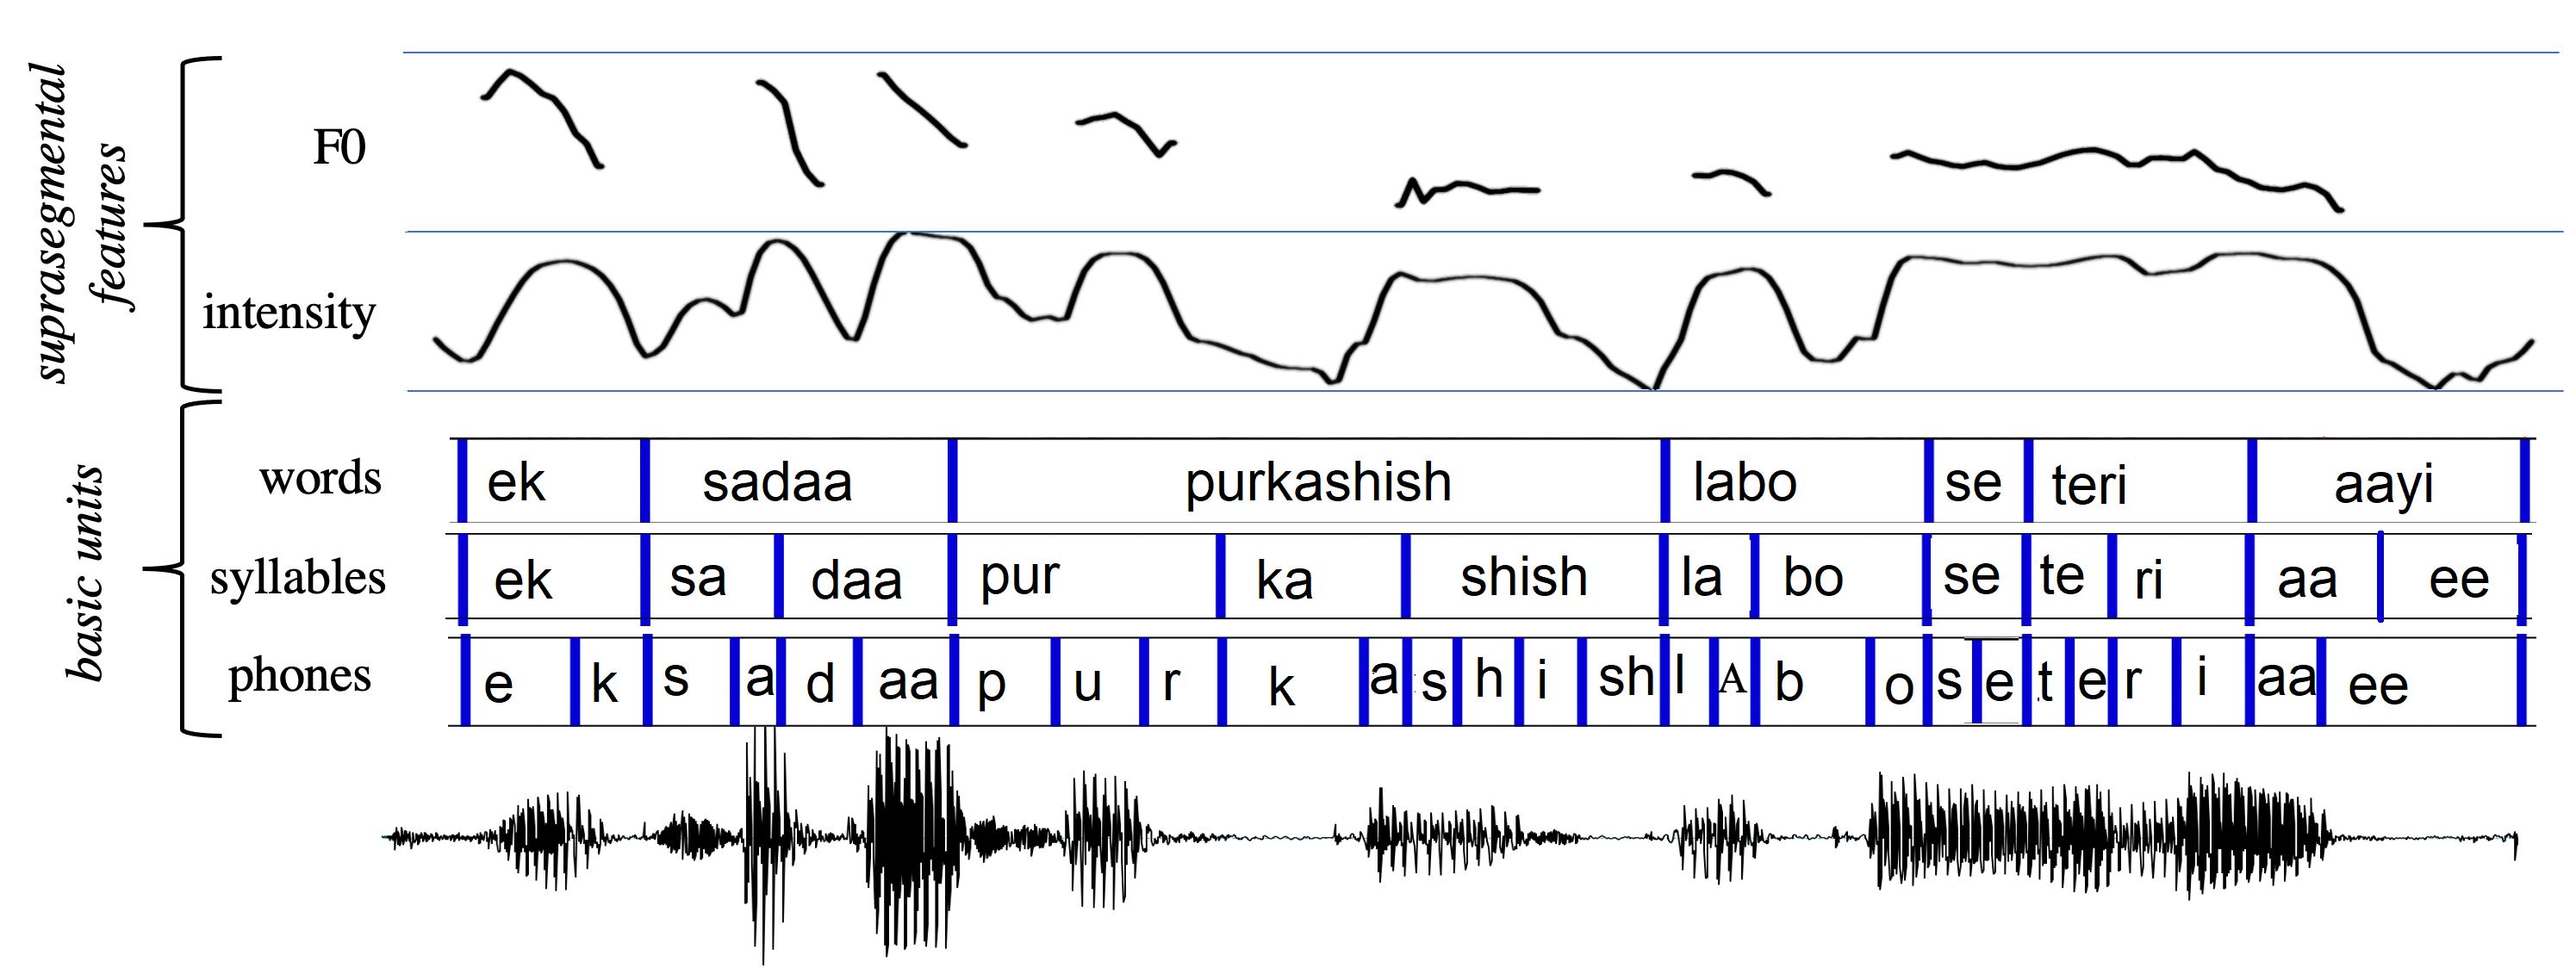
\includegraphics[width=0.9\textwidth]{img/speech3.png}
    \caption{Units of Language}
    \label{fig:units-of-language2}
\end{figure}

Going from lowest to highest units the structure is as follows \cite{brown_encyclopedia_2006}:
\begin{itemize}
    \item \textbf{Phones} are any distinct gesture or speech sound, irrespective of whether the exact sound is essentially required to provide meanings to words. 
    \item \textbf{Phoneme} is a speech sound in a given language that, if swapped with another phoneme could entirely change one word to other. They are the speech sounds that provide us the contrast of meaning between different words. For instance the English word 'cap' has 3 phonemes – 'c' 'a' and 'p'
    \item \textbf{Syllables} are organized sequences of phones. Words are made up of one or more syllables. Syllables are one or more sound sequences consisting of a \textit{syllable-nucleus} which is usually a vowel and an onset (optional initial sequences) and conda (final sound sequences), which tend to have consonant sounds. For instance the English word 'cook' has one syllable, and 'meeting' has two syllables.
    \item \textbf{Words} are the basic units of written and spoken linguistics which contain meaning in isolation as well as in broader context of sentence or a conversation, unlike isolated phones and syllables which carry no meaning on their own except for the cases of monosyllabic words (e.g. hey, Eh). 
    \item \textbf{Utterance} is the smallest un-paused speech production act by single speaker that is preceded by silence and followed by silence or a change of speaker, delineated by speaker change or by clear pauses and it comprises of one or more words. 
    \begin{itemize}
        %\item An utterance is a stretch of spoken language that is preceded by silence and followed by silence or a change of speaker. 
        \item Segments of the stream of speech sounds that make up an utterance are phonemes, morphemes, and words.
        \item  In spoken language utterance tend to differ from single words to longer word streams and grammatical constructs.
        \item Speech, unlike written language, consists of speaking acts of variable duration rather than clearly delineated clauses or sentences. %In contrast to written language, where a sentence is one grammatical expression with a communicated meaning, speech consists of speaking acts of variable duration rather than clearly delineated clauses or sentences.
        \item Speakers tend to use fillers, prolonged vowels, hesitations and filled pauses like “eh” or “umm” or "ah" or "err" to signal their intention continuation of their utterance, but require little time to re-organize their thoughts to formulate the subsequent speech in their mind.
        \item Some examples include saying "150" in math class to answer your teacher's question, Policeman yelling "Stop!", saying "Good boy!" to your pet dog, and even a long one hour speech by the President of a country.      
    \end{itemize}
     \item \textbf{Sentences} - Group of words that follow a coherent structure (syntax), following certain protocols (grammar) is called sentences that contain information and meaning (pragmatics).
\end{itemize}

Aside from the units of speech mentioned above, there are several other units and structural linguistic concepts used in linguistic theory that are less commonly used in speech processing. They do, however, come into play when mapping speech to written language or vice versa, or when using speech processing tools for linguistic research. An example of this type of area of linguistics study is called \textit{morphology} \cite{backstrom_introduction_2022}. 

\section{Speech Features Extraction Process}

Speech Features like frequency, amplitude, resonance, harmonics, pitch, tone etc as a whole can be holistically understood by humans but computers cannot understand them directly. Hence, we need to convert analogue speech signal to Digital. In Digital these nuanced information like frequencies, amplitude etc need to be in an understandable format for the computer. These dimensions need to be broken down in presentable form to make it easy for us to understand and work as well. 

\subsection{Audio Features}
Audio features can be categorized into following:
\begin{enumerate}
    \item High-Level Audio Features keys, chords, rhythm, melody, tempo, lyrics, genre, and mood.
    \item Mid-Level Audio Features include pitch and beat level attributes like MFCCs, Fbanks, CMVN, HEQ, note fluctuation patterns or the start of a musical note called note onsets.
    \item Low-Level Audio Features are generally the statistical features that get extracted from the audio which include amplitude envelope, energy, zero-crossing rate etc. 
\end{enumerate}

There are two main feature extraction and representation processes popularly used:
\begin{enumerate}
    \item Mel-Filter Banks
    \item Mel Frequency Cepstral Coefficients
\end{enumerate}

There is an ongoing debate in the ASR community about using the DCT instead of the log Mel fiter-bank features, especially for Deep Neural Network-based acoustic models \cite{raj_note_nodate}. Filter banks and MFCCs computation is done by almost same procedure; MFCC is calculated after a Cosine Transformation of FilterBanks.

\subsection{Mel-Filter Banks}

The signal goes through following steps to calculate Filter banks after Analogue to Digital Conversion \cite{backstrom_introduction_2022}: 
\begin{enumerate}
    \item Pre-emphasis filter.
    \item Signal Slicing into overlapping frames.
    \item Applying window function to each frame.
    \item Short-Time Fourier Transform or simply Fourier Transform on each frame for power spectrum calculation.
    \item Computation of filter banks. 
\end{enumerate}

Individual frequencies are difficult to distinguish in the raw power spectrum, especially at high frequencies.  To solve this, the spectrum is convolved with several (20-40, in general) triangular Mel filters, referred to as a filterbank, which is wider at higher frequencies because humans do not perceive loudness on a linear scale i.e. at higher the frequency, lower the perceived loudness. Thus these filters are narrow at low frequencies and widen as frequency increases \cite{raj_note_nodate}. The logarithmic scale of Mel-filterbank output is used to reduce the number of acoustic variants that are unimportant for speech recognition. 

Mel scale can be converted from frequency by following formula: \cite{backstrom_introduction_2022}:
\begin{equation}
    M(f)=1125\ln_(1+\frac{f}{400}) \\
\end{equation}
to go from Mels back to Frequency: \\
\begin{equation}
    M^{-1}(m)=700(exp(\frac{m}{125})-1) \\
\end{equation}

\subsection{Mel Frequency Cepstral Coefficient}

MFCC is the industry standard due to its good performance ever since Davis and Mermelstein developed MFCC in the 1980s. It can extract important information from speech signal and audio which is an active research area \cite{noauthor_mfcc_nodate}. 

Since filter-bank energies cannot be used directly with a Gaussian mixture with diagonal covariance and are correlated, they are de-correlated using DCT which is applied to the FBanks to retain a number of the resulting co-efficients while the rest are discarded to compute MFCCs. Mean normalization is applied after this by subtracting the mean of each coefficient from all frames, to balance the spectrum and improve SNR. 

\begin{figure}[h]
    \centering
    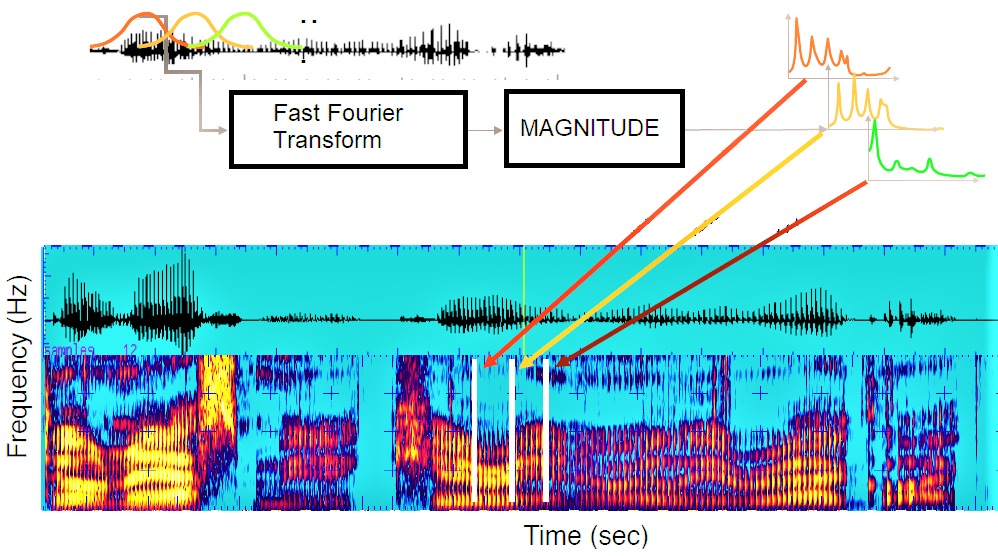
\includegraphics[width=0.8\textwidth]{img/feature extraction22.png}
    \caption{Feature Extraction Pictorial Representation}
    \label{fig:Feature-extraction-pic}
\end{figure}

%Some research groups, such as Google, use filter-banks (fbanks) \cite{noauthor_mfcc_nodate}. 

\begin{figure}[htb]
    \centering
    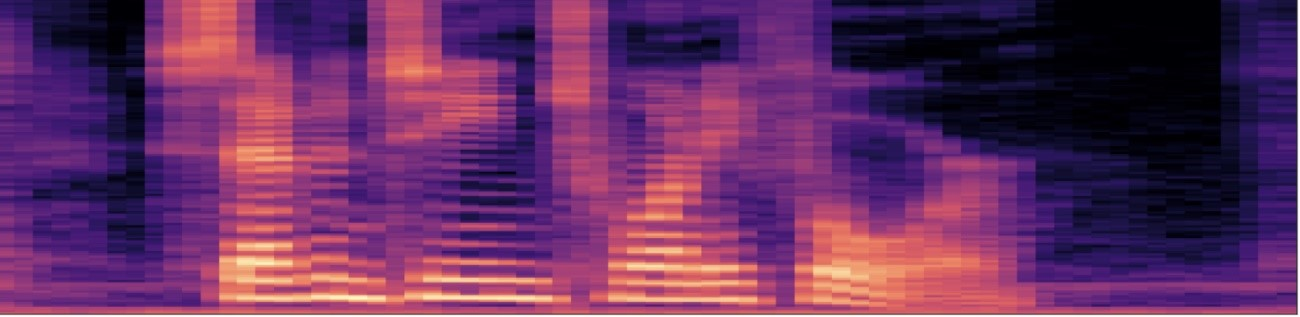
\includegraphics[width=0.7\textwidth]{img/mfcc4.jpg}
    \caption{MFCC - X axis represents time and Y Axis represents features}
    \label{fig:mfcc-example}
\end{figure}

\subsection{Comparing Mel FilterBanks and MFCCs}

The nature and human perception of the speech signal inspired all of the steps required to compute filter banks. The limitations in some ML algorithms  requirement of extra steps in MFCC computation. To de-correlate filter-bank coefficients, DCT is required. This process is also called whitening. MFCCs were popular when HMM-GMM were popular and they co-evolved to be the Standard ASR methods up till late 90s \cite{backstrom_introduction_2022}. 

However, with advancement of NNs and Deep Learning in ASR, Filterbank popularity increased because DNNs are less susceptible to highly correlated input which is why DCT was no longer required \cite{raj_note_nodate}. DCT  being linear transformation discards some information in speech signals which are highly non-linear and hence is considered undesirable \cite{fayek_speech_2016}.

It might be beneficial to attempt to learn directly from the signal in the time domain which has given promising results and bypass Fourier Transform since it is a linear operation and is a difficult operation to learn which may increase data and model complexity required for achievement of same performance. Signal is assumed to be stationary within this short time-frame when doing STFT, which is why the Fourier transform linearity does not pose much of a problem \cite{fayek_speech_2016}.

\section{How Does Computer Understand Speech?}
\label{sec:what-is-asr}

Automatic Speech Recognition refers to the technology that enables communication and interaction with computers using Speech \cite{lakshmi_sri_kaldi_2020}. Humans use their mouth, tongue, lips lungs and larynx to generate sound (emitter) and their ears capture the sound (receiver) which is then captured in the brain, analyzed, understood, and is then processed as thoughts or action. The computer however captures speech sound or audio using a microphone (receiver) and converts the analog signal of speech sound into digital audio so the computer can understand it by creation of a wave file of the spoken words and breaking down of these filtered wave files into phonemes \cite{backstrom_introduction_2022}. 

ASR systems generate the most likely word sequence from a given speech signal. ASR research was dominated by the statistical approach which gave good results. The speech recognition problem statement can be generally defined as \textit{"the conversion of spoken utterances into textual sentences by a machine"}. Bayesian decision rule is employed in this statistical traditional framework to produce the most likely word-sequence given the observation-sequence $O=(o_{1},o_{2}...o_{T})$ \cite{maglogiannis__2020}:

\begin{equation}
\centering
\hat{H} = \argmax_{H} P(H|O)    
\end{equation}

In accordance with Bayes' rule, posterior probability in the above-mentioned equation is expressed as \textit{"product of a conditional probability of the word-sequence given the acoustic observations i.e. P (O|H) and a prior probability of the sequence of words i.e. P (H), and normalised by the marginal likelihood of sequence of observations i.e. P (O)"} \cite{backstrom_introduction_2022}:

\begin{equation}
\centering
\hat{H} = \frac{\argmax_{H} P(O|H) P(H)} {P(O)}
= \argmax_{H} P(O|H) P(H) 
\end{equation}

The marginal probability i.e. P(O) in second equation is omitted because it is constant w.r.t the ranking of hypotheses and thus has no effect on the search for the best hypothesis. The acoustic model calculates P(O|H), while the language model models P(H) \cite{backstrom_introduction_2022}.

\section{Components of Automatic Speech Recognition System}
\label{sec:components-of-asr}

\begin{figure}
    \centering
    %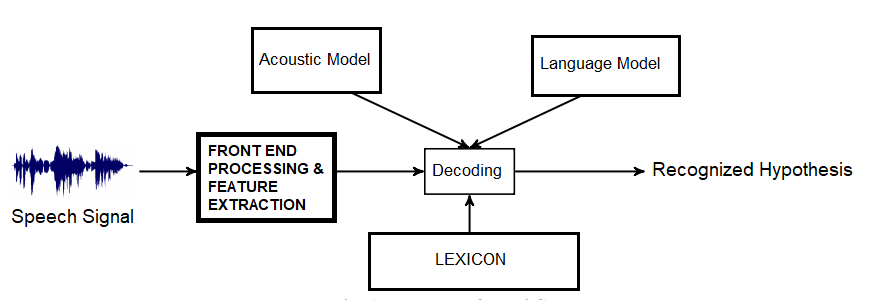
\includegraphics[width=0.8\textwidth]{img/ASR-diagram2.png}
    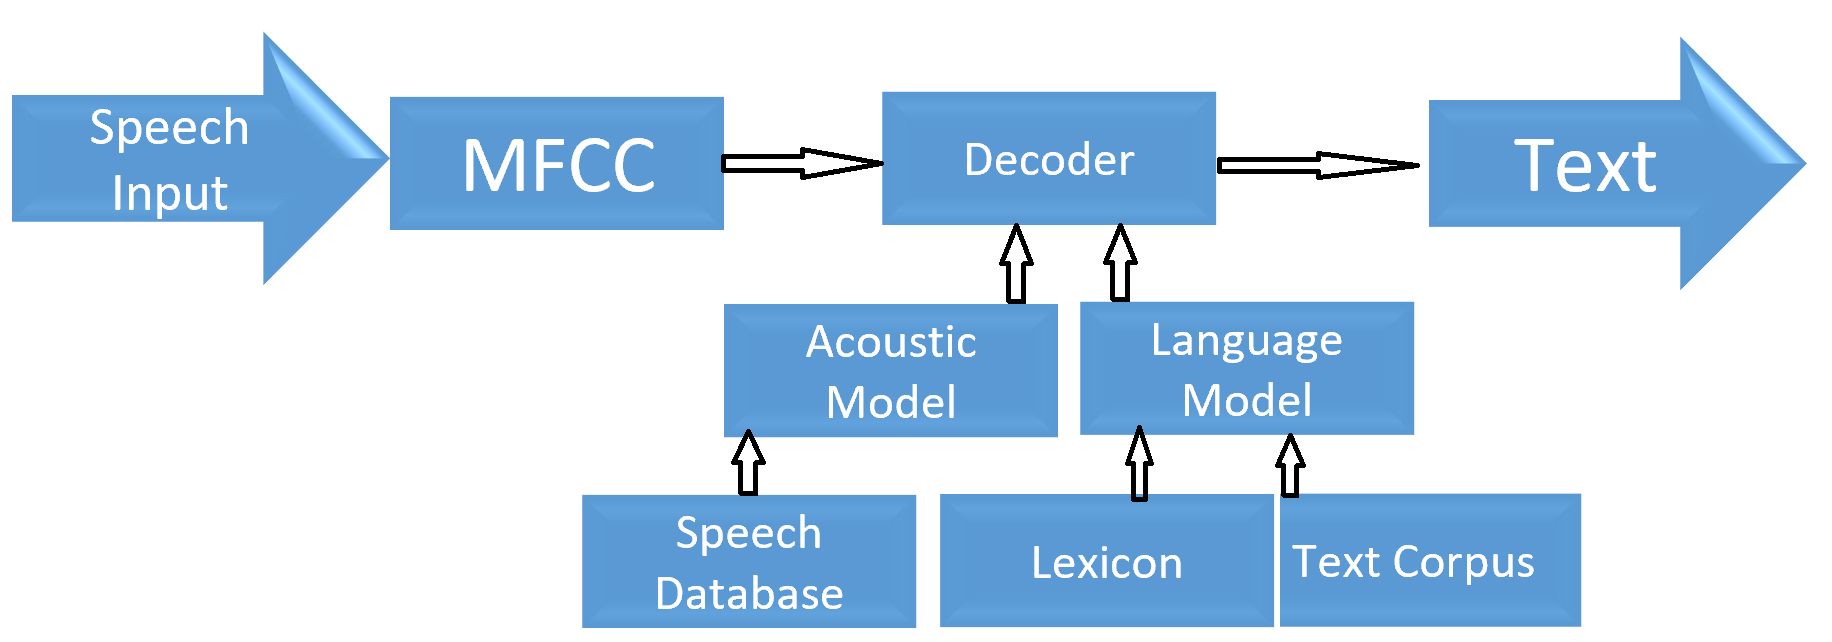
\includegraphics[width=0.7\textwidth]{img/traditional.png}
    \caption{Basic Traditional ASR Architecture}
    \label{fig:asr-diag-arch}
\end{figure}

%\begin{figure}[h]
%    \centering
%    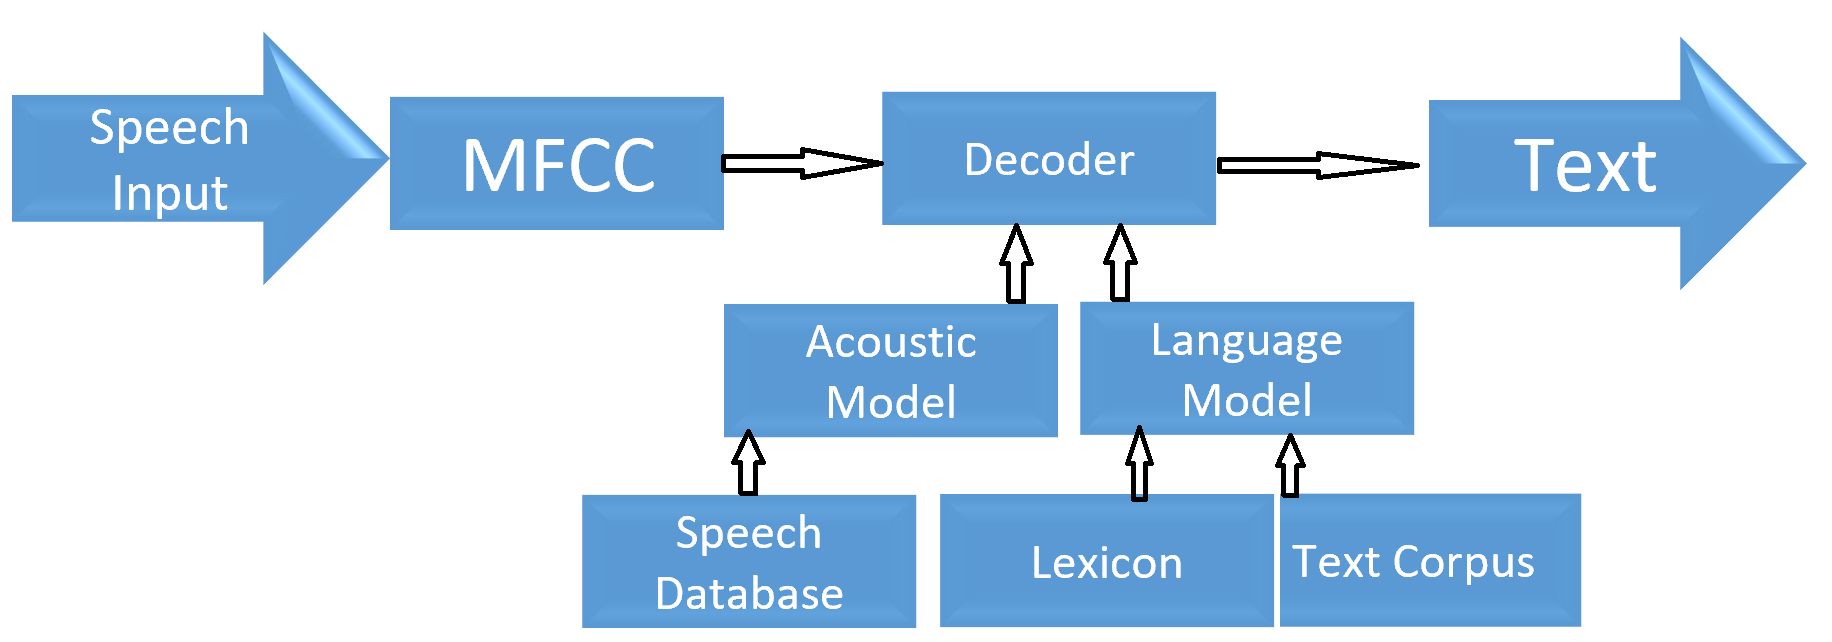
\includegraphics[width=0.7\textwidth]{img/traditional.png}
%    \caption{Traditional ASR}
%    \label{fig:trad-asr}
%\end{figure}

An ASR application takes speech signal input to convert it into a sequence of words in text form as output. During the speech recognition process, a list of possible texts is generated, and the most relevant text to the original sound signal is selected \cite{davis_automatic_1952}. The basic ASR system architecture is given in Figure \ref{fig:asr-diag-arch}.

The vocabulary of ASRs increased to 1000s of words from a few hundred in the 1980s thanks to a new statistical method called "Hidden Markov Model (HMM)," which estimated the probability of unknown sounds actually being words rather than just using words and looking for sound patterns \cite{suma_swamy_evolution_2013}. For a long time, the HMM-GMM was regarded as the standard model for large vocabulary continuous speech recognition (LVCSR), producing the best results.

Statistical models give better performance on low-resource languages with speech data of around 10-30 hours \cite{naeem_subspace_2020}. They offer a strong mathematical foundation, effective learning and decoding techniques, good sequence abstractions, temporal aspects, and flexible topology for statistical phonology and syntax \cite{morgan_continuous_1995} %They provide a Rich mathematical framework, Powerful learning and decoding methods,good abstractions for sequences, temporal aspects and flexible topology for statistical phonology and syntax.

In general ASR systems have following main components \cite{maglogiannis__2020}:

\begin{enumerate}
    \item \textbf{Front End:} Here the speech signal is accepted as input and is sent to relevant modules to extract useful features\cite{s_review_2016}.  
    \item \textbf{Feature Extraction:} The input speech signal is converted into a sequence of acoustic feature vectors or observations which are compact and contain information for later stages of recognition. Some spectra-temporal analysis of the signal generates features that typically transform into more compact and robust vectors %Common feature vectors include Principle Component Analysis (PCA), Linear Discriminant Analysis (LDA), Independent Component Analysis (ICA), Linear Predictive Coding (LPC), Cepstral Analysis, Mel-Frequency Scale Analysis, Filter-Bank Analysis, Mel-Frequency Cepstrum Coefficients (MFCC), Kernel Based Feature Extraction, Dynamic Feature Extraction, Wavelet-based features; Spectral Subtraction and Cepstral Mean Subtraction (CMS) 
    \item \textbf{Language Model:} It contains a lexicon of words and their likelihood of occurrence in a given sequence (in a corpus). It includes terms from the current application's or context's vocabulary. It specifies the constraints associated with the sequence of words accepted in a given language. %Commonly used tools for language modelling are the CMU Statistical Language Modeling (CMU-SLM) Toolkit and the Stanford Research Institute Language Modeling Toolkit (SRILM) \cite{maglogiannis__2020}.      
    \item \textbf{Acoustic Model:} It consists of acoustic features for each distinct phonetic units, referring to the process of establishing the statistical representations for the feature vector sequences computed from the speech waveform i.e. it contains a statistical representation of the distinct sounds forming these words in the grammar or the overall Language Model. Each distinct sound corresponds to a phoneme. The acoustic lexicon and language model are used in the processing stage by a search algorithm or decoder to produce the hypothesised phoneme or word. %The Commonly used Acoustic Modelling methods are Hidden Markov Models, Segmental Models, Super Segmental Models, Neural Networks (Deep Neural Network, Recurrent Neural Networks, Convolutional Neural Network, Time Delay Neural Network and CNN-TDNN), Maximum Entropy Models and Conditional Random Field.    
    \item \textbf{Decoder:} This software searches the acoustic Model for equivalent sounds to the sounds spoken by a speaker. The decoder determines the phoneme associated with that sound when a match is discovered. It keeps track of the phonemes that match until there is a pause in the speaker's speech. The language model is then searched for the equivalent phoneme series or sequence. It gives the text of the corresponding word or phrase as output when a match is found. The decoder tries to find the most likely sequences of words matching the audio signal by applying appropriate models. Most commonly, decoder algorithms produce the \textit{n-best list} which is the list of possible sequence of words. 
\end{enumerate}    
For Scoring and Evaluation, we use string edit distance to determine how accurate our speech recognizer is. To align ASR output with reference transcription, we use dynamic programming. Insertion, deletion, and substitution are the three types of errors and one way to address these types of errors are by calculating WER. If reference transcripts contain N words and ASR output contains "S" substitutions, "D" deletions, and "I" insertions, then \cite{morris_wer_2004}:

   \begin{equation}
       WER = 100.\frac{W+D+I}{N} \% \quad \quad Accuracy = 1-WER \%
   \end{equation} 

ASR engines have their own scoring scripts which compare its transcription with the ones provided by users as references and scores it as Word and Sentence Error Rates. Release of new test sets based on common training and development data on which different systems can be evaluated using WER. A WER of 5\% roughly corresponds to one missed word out of every twenty. If each sentence contains 20 words (which is about average for English), the sentence error rate could reach 100\% \cite{patil_automatic_2016}.

\section{Types of ASR}
\label{sec:types-asr}
In terms of application of ASR systems the types of ASR include \cite{backstrom_introduction_2022}:
\begin{enumerate}
    \item Voice Activity Detection
    \item Speech to Text
    \item Text to Speech
    \item Voice Identification
    \item Speech Enhancement
    \item Speaker Diarization
    \item Wake Word Detection
    \item Para-linguistic Speech Processing and Analysis (Speech Emotion Recognition)
\end{enumerate}

\section{Uses of ASR}
\label{sec:uses-of-asr}
Some common uses of ASR are as follows \cite{backstrom_introduction_2022}:
\begin{itemize}
    \item Quality of Service
    \item Speech Transcription or Dictation services
    \item Call monitoring, transcription and analysis
    \item Speaker identification for secure premises
    \item Subtitle generation for streaming services
    \item Vocalist and Instrument recognition in songs
    \item Medical uses e.g. detecting Alzheimer \cite{konig_automatic_2015}, speech disorders, stress etc.
\end{itemize}






    %!TEX root = ../thesis.tex

\chapter{Challenges in ASR and Role of AI in \\ Speech Technology}    % (fold)
\label{cha:why_asr_difficult}

There are more than 6,000 languages globally out of which, only in Europe, 24 are official languages, 5 semi-official languages, and more than 100 additional regional or minority languages with more than 50 million language speakers in Europe if we rank the top 50 languages. Currently, 3,000 different languages are considered to be endangered. The figure \ref{fig:lang-vocab-1} and \ref{fig:lang-vocab-2} show the number of unique and new words in various languages \cite{creutz_morph-based_2007}. Each Language requires a separate language model for Speech Recognition which in turn requires big data. Hence ASR for Low-Resource Language is a serious challenge in this field \cite{besacier_automatic_2014}. 

\begin{figure}[h]
    \centering
    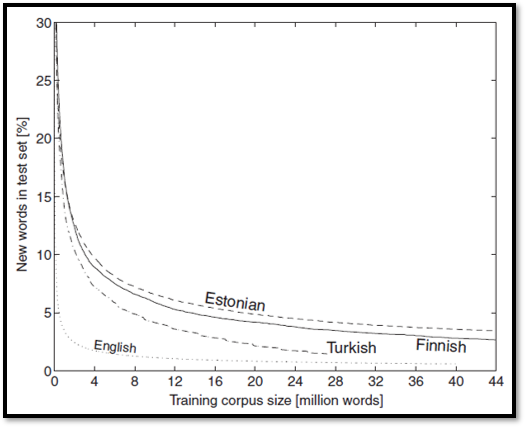
\includegraphics[width=0.5\textwidth]{img/Creutz.png}
    \caption{Languages and Vocabulary (New words) \cite{creutz_morph-based_2007}}
    \label{fig:lang-vocab-1}
\end{figure}

\begin{figure}[h]
    \centering
    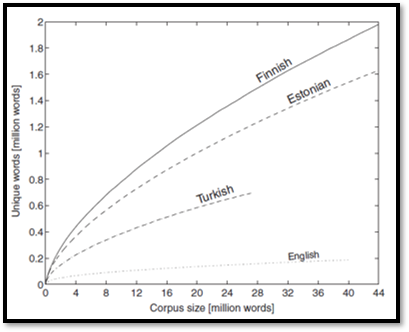
\includegraphics[width=0.5\textwidth]{img/Creutz2.png}
    \caption{Languages and Vocabulary (Unique words) \cite{creutz_morph-based_2007}}
    \label{fig:lang-vocab-2}
\end{figure}

Although ASR research has progressed significantly, but has not reached perfection. Speech recognizers are not very robust and make mistakes for a variety of reasons. We will delve deeper into each type of problem in the ensuing subsections.

\section{Speaker Variation Problems}
\label{sub:speaker_variation}
There are factors with regard to type of speaker which affect the audio information. Following must be catered with regards to Speaker Variation which affects Acoustic Modelling:
\begin{itemize}
    \item \textit{Vocal range} e.g. fundamental frequency, and pitch range \cite{vipperla_ageing_2010}. 
    \item \textit{Speed and length of speech} e.g. This must be planned when training data-set i.e. whether we want to train on isolated or continuous speech \cite{markus_forsberg_why_2003}. 
    \item \textit{Quality of Voice} like whisper, grunt, growl, physiological elements e.g. nasality, adenoidality, etc \cite{shrawankar_adverse_2013}. 
    \item \textit{Accent and dialects}, e.g.vowel systems, consonants, allophones, etc.) which may make it difficult of ASR to recognize words \cite{shrawankar_adverse_2013}. 
    \item \textit{Health, emotional state} etc which can be problematic in speaker verification systems \cite{backstrom_introduction_2022}.
    \item \textit{Speech style} - It is more difficult to build a speech recognizer that recognises only formally read speech than the one that allows the user to speak spontaneously because spontaneous speech is characterised by incomplete sentences, false starts, extended words, poor pronunciation quality, and an infinite vocabulary. \textit{Disfluencies} in spontaneous speech like long pauses, fillers, false starts, hesitations, ungrammatical constructions, and mispronunciations are the primary cause of the difference in recognition error rates between spontaneous and read-out speech. Hence, acoustically and grammatically it is difficult to recognise spontaneous speech \cite{shrawankar_adverse_2013}.
    \item \textit{Prosody} – Stress, intonation, and rhythm convey critical information for word recognition and the user's understanding. These stresses can cause the words to change e.g. in Arabic, the "shad" notation means more stress \cite{shrawankar_adverse_2013, markus_forsberg_why_2003}. So the word Becca with stress on "cc" part will sound different. ASRs face issues recognizing these differences.
    \item \textit{Type of Utterance} -  Every word recognised by a speech recognizer may be recognised independently. It might ask the user to speak each word of the sentence with a fake pause in between, or let them speak normally. There are two different systems in this way:
    \begin{itemize}
        \item \textit{Isolated word recognition system} is the most fundamental recognition strategy which is possible to develop without an LM by using word-based acoustic models. Sentences made up of isolated words become more difficult to recognize as the vocabulary grows, necessitating the usage of sub-word based language and acoustic models \cite{backstrom_introduction_2022}.
        \item \textit{Continuous speech recognition systems} enables users to express themselves in a comparatively or fully unrestricted manner. These recognizers, in presence of all co-articulatory effects, must give a good performance. As a result, development of Continuous Speech Recognition is arduous because word boundaries are ambiguous, and co-articulatory effects are much stronger in continuous speech \cite{markus_forsberg_why_2003}.
    \end{itemize}
   
\end{itemize}

\section{Linguistic Issues}
\label{sub:linguistic-issues-asr}
Linguistic issues make ASR difficult as in this domain following must be catered for:

\begin{itemize}
    \item \textit{Out-of-vocabulary (OOVs)} - Jargon, slang etc are OOVs which are are hard problems of ASRs. 
    \begin{itemize}
        \item The most advanced ASRs on the market today have limited vocabularies and cannot recognise words outside of their training vocabulary.
        \item  For HMM-GMM and neural ASR systems, special techniques for handling OOV words are available for deployment. \cite{zhang_strategies_2019}.
    \end{itemize}       
    \item \textit{Homophone Substitution} - Generally, a well-functioning language model should be able to distinguish homophones based on context. Homo-phonic substitution errors can occur where multiple lexical entries with the same pronunciation or phone sequence called homophones exist. During decoding, homophones cause confusion with one another, resulting in errors, such as the distinction of disambiguation homophones such as "their" and "there" or "hear", "here", "hare" and "hair" \cite{vasilescu_cross-lingual_2011}. %Homophonic substitution in an input utterance confuses the system with a similar word or homophones in its own vocabulary leading to misunderstandings. 
    \item Recognition of \textit{children’s speech} and of \textit{people with speaking disorders} is sub-optimal with standard corpus or any regular kind of training data \cite{kumar_leveraging_2020}.
    \item \textit{Consideration for linguistic structure} i.e. phonetics, morphology, graphemes, etc \cite{creutz_morph-based_2007, backstrom_introduction_2022}. 
    \begin{itemize}
        \item Many languages have a greater morphological richness than English, which has an impact on vocabulary construction and language modelling.
        \item Compounding is used in languages such as German in which compound words are decomposed into constituent parts and then pronunciation and language modelling are performed on the decomposed parts.
        \item All morphology-based approaches aim to reduce ASR errors by reducing the OOV rate through modelling at the morph level, while also accounting for the lack of broad-vocabulary data, as we are not always able to arrange an audio data-set for every word in the dictionary. 
        \item Morphs are used instead of words in morph-based language modelling, but the context may need to be extended because multiple morphs are related to a single word \cite{creutz_morph-based_2007}.
    \end{itemize}  
    \item \textit{Code-Switching} - Often in many areas, no one speaks the particular language purely which is why we need a mix of out-of-language words in the lexicon from other languages \cite{farooq_enhancing_2020}. E.g. in Pakistan, Urdu may be the official language but no one speaks pure Urdu. It is often mixed with some words from English, Panjabi, Hindi, Sindhi and Pashto. This is an issue which we will discuss further in Section \ref{sub:code-switching-problem}. 
\end{itemize}

\subsection{Code-Switching Problem}
\label{sub:code-switching-problem}

Code-Switching is spontaneous use of more than two languages in a single sentence or the whole conversation. It a linguistic phenomenon prevalent in multi-cultural societies as well as in the countries where official language and native language are different e.g. in Pakistan its English and Urdu and in case of Algeria and Tunisia it is French and Arabic etc. It is also an active research area in ASR \cite{farooq_enhancing_2020}.

The following sentence is an example of what types of calls we get in CPLC call center which can be referred to as Urban or code-switched Urdu: 
\begin{quote}
\textit{"Assalamualaikum mujhe urgently aik report darj karani he"}    
\end{quote}

The sentence can be translated in English as \textit{"Peace be on You. I want to urgently file a report."}
\vspace{11pt}
\par
Let us observe the original sentence that has multiple code switches. The first word \textit{"Assalamualaikum"} is a common Muslim greeting that is basically an Arabic word. The next word \textit{mujhe} is an Urdu word followed by an English word, Then urdu, then English and last three words again are Urdu words. For transcription  we kept Roman script instead of Nastaliq for Urdu and Roman for English so that we do not have to do separate language modeling for every language word that occurs in the corpus.

\section{Model Training and Deployment Challenges}
\label{sub:model-training_asr_difficult}

Every language needs a different language model. There are approximately 7,000 languages in the world, the majority of which have limited training resources, code-switching issues, and language change issues, and we cannot create a one-size-fits-all model for them. That requires us to train model for each language as per the scenario \cite{pironkov_hybrid-task_2020}.

Some more factors we need to cater are:
\begin{itemize}
    \item \textit{Robustness} i.e. ability to work despite small errors, having graceful degradation and not catastrophic failure \cite{shrawankar_adverse_2013}.
    \item \textit{Portability} i.e. ease of deployment, independence of computing platform etc \cite{kincaid_state_2018}.
    \item \textit{Adaptability} to changing conditions e.g.  telephonic environment, gender, different speaker, mic, noisy conditions, or even new language etc \cite{kincaid_state_2018}.
    \item \textit{Confidence} Measures i.e. methods to evaluate correctness of hypothesis \cite{backstrom_introduction_2022}.
    \item \textit{Computational} power requirement like GPU, Processors, Electricity availability \cite{kincaid_state_2018}.
    \item \textit{Financial Costs} including hardware, software and HR. Apart from the scale of data, we also need to consider the cost of building applications which are mostly fixed, and don’t scale with the size of our profit. The scale at which we can break even will tend to decrease over time, as the algorithms get better, and the software becomes easier to use but the cost of the training data will still be less than what is paid to ASR engineers \cite{kincaid_state_2018}.
    \item \textit{Availability of Skills} which includes data-scientists and AI Engineers for Speech Processing \cite{kincaid_state_2018}.
    \item \textit{Speaker-independent or Speaker Tuned for a particular speaker} e.g. in case of speaker dependent system, adaptation to speaker characteristics is key \cite{shrawankar_adverse_2013}.
    \item \textit{Hierarchical and Compositional nature of speech production and comprehension} makes it difficult to handle with single model. The decoder may be forced to reject the true hypothesis in favour of a spurious candidate with high language model probability due to an undue Language model bias caused by a high relative weight on the language model. These errors could occur in tandem with analogous acoustic model bias \cite{backstrom_introduction_2022}.     
    \item \textit{Spectral Bandwidth} i.e. with decrease in bandwidth, the performance of the trained ASR system will also decrease, and vice versa.
    \item \textit{Variable Environmental noises} reduce accuracy of ASR \cite{misra_spectral_2004}.
    \item \textit{Overlapping speech} is still a hard problem for ASR system in production environment \cite{chen_progressive_2018}.
    \item \textit{Type Of ASR Approach} to be taken is an important consideration \cite{georgescu_performance_2021}. On lesser data Deep Learning is not as effective as traditional but on larger data-set, we find Deep Learning to improve the accuracy indefinitely (See figure \ref{fig:comparison-all-asr-approach}). 
    \item ASR as a \textit{classification problem} has very high dimensional output space \cite{jurafsky_speech_2009}. 
    \item ASR as a \textit{sequence-to-sequence problem}, has a very long input sequence although limited reordering between acoustic and word sequences \cite{jurafsky_speech_2009}.
\end{itemize}

\section{Data-set Challenges}
\label{sub:data-set-asr_difficult}

\begin{itemize}
    \item \textit{Availability of Data-set} - This is one of the biggest issue for ASR researchers especially in case of low-resource languages. Data available on internet e.g. on Kaggle, GitHub, YouTube etc wouldnot work in every scenario. Sometimes we need Code-switched dataset which adds to problem of availability of dataset \cite{besacier_automatic_2014}.
    \begin{itemize}
        \item Availability of big data is often thought as having a huge database of audio files and it is a common misconception. Big data refers to availability of high quality labelled big amount of data. 
        \item Not everyone will have the access to big amount of Labelled data. Often people consider availability of data as big data without considering if it is labelled accurately or not.  
        \item If the system depends on ten thousand hours of data, it is not deployable every where because the right data type is usually not available at large scale. There are various papers claiming great performance on Switchboard Eval2000 corpus i.e. with thousands of hours of data but it does not really take the field of ASR forward. 
        \item For an application requiring have a well-labelled training data, which is the case with most applications, best plan is to make it work well when trained with 10 hours of data, so that we can build a prototype with reasonable performance allowing us to scale our data up or to get funding, investment or sponsorship \cite{kincaid_state_2018}.
    \end{itemize}   
    \item \textit{Vocabulary Size} - The number of words in a speech recognition system's vocabulary is a limitation \cite{zhang_strategies_2019}. 
    \begin{itemize}
        \item \textit{Small Vocabulary Systems} have around 1-99 words
        \item \textit{Medium Vocabulary Systems} have around 100-999 words
        \item \textit{Large Vocabulary Systems} have 1000-plus words and there are some challenges with these systems: 
        \begin{itemize}
            \item LVCSR systems performs worse than small vocabulary systems due to factors like word confusion which increases with the number of words in the vocabulary. 
            \item A small vocabulary recognizer can individually model each word, but training acoustic models for thousands of words at once is impractical due to lack of training speech data and storage for necessary speech parameters, due to which sub-word units are required to be used which degrade performance because they cannot capture co-articulatory effects like words-based units do \cite{backstrom_introduction_2022}. 
            \item The search process in a large vocabulary recognizer implements pruning (model size reduction by removing non-critical and redundant portions for better classification) rather than a full search \cite{backstrom_introduction_2022}.
        \end{itemize}               
    \end{itemize}    
    \item Machine-directed commands, scientific language, colloquial expressions, and other more nuanced words and expressions like emojis continue to pose difficulties for Speech Recognition Systems \cite{jurafsky_speech_2009}. 
    \item \textit{Multiple acoustic problem} - This is a broad category of errors that include those caused by bad pronunciation entries in the data-set; speaker mispronunciation, disfluency or acoustic models' errors, possibly because of data mismatch between training and usage or data mislabelling, acoustic noise etc \cite{backstrom_introduction_2022}.
    \item \textit{Data specific to environment} - At times we need environment specific data in addition to clean data like in a call centers scenario, we require noisy/telephonic audio data \cite{shrawankar_adverse_2013, schuller_recognition_2009}. 
    \begin{itemize}
        \item In comparison to text-based NLP, there is a scarcity of training data (in terms of words). 
        \item Data is quite often noisy, with numerous nuisance factors of variation. 
        \item Even if a large audio data bank is available, it must be labelled for training purposes. 
        \item Manual speech transcription is extremely costly (10x real-time). 
    \end{itemize}
    \item Open source Projects like Mozilla Common Voice may be collecting audio data in various languages including Urdu and providing it for free. This is a very noble cause and can help many beginners to learn ASR, but it is not a one size fits all data. It may make a good voice command system for voice assistants but if we want to build a recognizer to process call center conversations in code-switched Urdu, Panjabi, Hindi, and Indian-accented English, or one that can deal with commands inside a car, the Mozilla Common Voice or Kaggle data-set is not going to help \cite{kincaid_state_2018}.
    \item \textit{Noisy Dataset Problems} - ASR may require that the speech be free of environmental noises, mic sounds, transmission channel and acoustic distortions, or it may be able to deal with any of these issues \cite{schuller_recognition_2009}.
        \begin{itemize}
            \item A critical issue for ASR system when working in a telephonic call centre environment is distinguishing speech from background noise which includes speech from other speakers, equipment sounds, fans, air conditioners, background voices, a bad microphone, speaker making noise by smacking his or her lips, coughing, or sneezing 
            \item ASRs presently are usually tested clean or controlled environments where they perform well but their performance rapidly degrades in noisy environments. 
            \item Speech overlapping is another key issue which is caused by multiple people speaking over each other at the same time. In presence of cross-talk in a speech signals ASR performance decreases significantly \cite{alharbi_automatic_2021}.
        \end{itemize}     
\end{itemize}

\subsection{Security and Privacy in Speech Research}
\label{sub:security_privacy_asr_research}

Scientific research is founded on evidence-based arguments. In the Science and Technology of Speech, audio recordings of speech are the evidence and the data. Hence, for any Speech Technology researcher, access to speech data is elementary and in our case, we had the access to telephonic audio data. 

To obtain consistent and accurate results, various independent researchers must be able to verify each other’s results. This requires that they have access to the same or nearly identical data sources; otherwise, we will be unable to demonstrate reproducible research. While shared data is regarded as the gold standard for reproducible research, sharing speech data can be problematic due to speaker privacy concerns \cite{noauthor_spsc_nodate}.

Data sharing is permissible if an individual is not uniquely identifiable in a data set. As a result, we kept our model speaker-independent so that it could be deployed anywhere without fear of information leakage. However, in the context of what constitutes identifying data, it is unclear what makes that data "uniquely" identifying. When new information is published and new technologies emerge, the nature of unique identifiability can change over time. This means that previously adequately protected data-sets become vulnerable to privacy issues over time. Hence, it is critical that researchers monitor their published data-sets over time so that they can take appropriate action if new threats emerge like withdrawing a data-set entirely.Reasonable approaches to implementing this could include \cite{backstrom_introduction_2022}:

\begin{itemize}
    \item \textit{Expiry date} - All data-sets should have a clearly defined shelf-life, after which the use of that data should be prohibited. If no new threats are discovered, the data-set's manager could update the expiry date. Consequently, academic papers based on expired data-sets should be rejected.
    \item\textit{Controlled data-sets access} - For enforcement of purpose binding and enabling of data-set withdrawal, the data manager can mandate that all users register and sign a formal contract outlining accepted uses.
    \item \textit{On-site processing of highly sensitive data} - We can construct a computing architecture in which data is stored on a secure server and researchers have access to it via a secure API. Data never leaves the server, ensuring that privacy is always maintained. Data can be stored on an air-gapped computer system for an even higher level of security, i.e. access to the data requires researchers to come physically to the computer, with no network access. Military Grade Systems use this grade of security \cite{backstrom_introduction_2022}.
\end{itemize}

Thus, in the context explained above, the Open source audio data-set is very limited for ASR training and the problem worsens for Low Resource Languages. 

\section{ASR for Low Resourced Languages}
\label{sec:ASR_for_Low_Resourced_Languages}

Languages having less web presence, linguistic expertise and digital resources like acoustic and text corpora, labelled audio data, pronunciation-lexica etc. are be defined as Under-Resourced or Low-Resourced Languages \cite{besacier_automatic_2014}. There are challenges with Low resource languages which are (not limited to) as follows:
\begin{itemize}
    \item Training acoustic and language models with sparse training data.
    \item Knowledge transfer between languages.
    \item The difficulty of creating a pronunciation lexicon.
    \item Language-specific characteristics e.g. morphology \cite{besacier_automatic_2014}.
\end{itemize}

%Urdu is Pakistan's "lingua franca," connecting people who speak regional languages such as Balochi, Pashto, Punjabi, and Sindhi with various dialects. It is spoken by over a hundred million people in Pakistan, India, Bangladesh, and parts of Europe. 

%Despite all this, Urdu is a low resource language because there is very little publicly available transcribed speech data, text corpus, and pronunciation lexicon. A robust speech recognition system generally requires hundreds of hours of transcribed speech data, as well as a massive text corpus and lexicon. As a result, Urdu speakers are excluded from the benefits of ASR.

%Under-Resourced Languages have recently been given some attention as highlighted by \cite{besacier_automatic_2014}. Before 2000s, HMM-GMMs were popularly used technique for developing acoustic models for speech recognition systems. However, with the resurgence of deep learning in 21st Century, the paradigm has shifted toward acoustic and language models based on Deep Neural Networks (DNN) in which HMM-generated alignments are used to train DNN-based acoustic models.

%Furthermore, RNNLMs are replacing widely used n-gram Language Models (LMs). \cite{meyerjosh_multi-task_2019} provides some interesting solutions methods to improve accuracy of under-resourced language ASR which involved use of knowledge of linguistic structure, improving ASR pipeline, using unsupervised clustering, reducing dependencies to structure using E2E Methods and Multi-Task Transfer Learning. 

\subsection{Why ASR for Low Resourced Languages need to be built from scratch?}
\label{sub:ASR_from_scratch}

Customized ASR solutions are very expensive and not every organization can afford them. Google’s ASR models are very good, but they won’t customize their models for any specific scenario. Their service is costly, and sometimes there are privacy issues \cite{zhou_security_2010} that preclude the use of a cloud service \cite{kumar_systematic_2020}, \cite{karimov_cloud_2021}. We also cannot expect them to cater for every scenario since no ASR is a one size fits all solution \cite{kincaid_brief_2018}. 

In case of Urdu, specifically, the type spoken in the Urban area also referred to as code-switched Urdu, there is no Model available which can be readily deployed in a noisy Telephonic Environment easily. While work may be available in Languages similar to Urdu like Hindi Language but it is not the optimum solution to implement in the Urdu environment although work on Hindi has been widely done. It’s hard to build a general-purpose model that will work as well as a model built for our specific task i.e., Code-switched Urdu ASR for call center/ telephonic environment \cite{kincaid_state_2018}. 

Organizations like Linguistic Data Consortium \cite{garofolo_john_s_csr-i_2007} and Al-Khwarizmi CLE \cite{noauthor_center_nodate} have data available with them but they are not open-source due to various concerns mentioned in Chapter 2. CommonVoice \cite{noauthor_mozilla_nodate} and Kaggle \cite{noauthor_kaggle_nodate} have some open source labeled Urdu data available but it does not suffice for our uses. However, it will be incorporated into our data-set to add as much depth and variety of vocabulary as possible.

Since there are no pre-built solutions available for Low Resourced Language (especially for Urdu) for noisy call center scenario, ASR System for Under-Resourced Languages need to be built from scratch.

%%%%%%%%%%%%%%%%%%%%%%%%%%%%%%%%%%%%%%%%%%%%%%%%%%%%%%%%%%%%%%%%%%%%%%%%%%
%%%%%%%%%%%%%%%%%%%%%%%%%%%%%%%%%%%%%%%%%%%%%%%%%%%%%%%%%%%%%%%%%%%%%%%%%%
%%%%%%%%%%%%%%%%%%%%%%%%%%%%%%%%%%%%%%%%%%%%%%%%%%%%%%%%%%%%%%%%%%%%%%%%%%
%%%%%%%%%%%%%%%%%%%%%%%%%%%%%%%%%%%%%%%%%%%%%%%%%%%%%%%%%%%%%%%%%%%%%%%%%%

%\chapter{AI in Speech Recognition}

\section{Artificial Intelligence in Speech Processing}

%We will now discuss role of Neural Networks and AI in Speech Recognition followed by the three mainstream categories of ASR training approaches \cite{georgescu_performance_2021, backstrom_introduction_2022} i.e. Statistical or Traditional ASR, End to End ASR and Hybrid HMM-DNN.

Early ASRs were built using Statistical Techniques out of which HMM-GMM were most used till end of 1990s. However there were some limitations to the traditional method \cite{backstrom_introduction_2022}:

\begin{itemize}
    \item \textit{Complex Training and global optimization process -} Traditional HMM-based models frequently use a variety of training methods and data sets to train various modules, each of which is independently optimised with its own optimization objective functions which are generally distinct from the true LVCSR performance evaluation criteria. As a result, the optimality of each module may not result in global optimality, and joint loss optimization is not included \cite{naeem_subspace_2020}.
    \item \textit{Conditional independence assumptions -} Traditional HMM models use conditional independence assumptions within HMM and between various modules to simplify model construction and training which does not correspond to the actual LVCSR situation. \cite{backstrom_introduction_2022}.
    \item Language and Acoustic model optimizes only their own local output, requiring a lot of manual engineering to obtain good performance overall \cite{naeem_subspace_2020, backstrom_introduction_2022}.
    \item GMMs are inefficient for nonlinear class boundaries because they assume each frame is generated by a single component of the mixture \cite{bell_adaptation_2021}
\end{itemize}

Neural networks in ASR were first applied to build HMM-NN hybrid systems, which estimated or scaled likelihoods that act as the HMM state observation probabilities using Neural Network. Hybrid systems in 90s used feed-forward networks and recurrent neural networks (RNNs) achieving almost state-of-the-art results \cite{morgan_continuous_1995}. 

In Traditional Acoustic Modelling, the observation probability is generally represented by GMM where as the DNN method in Hybrid HMM-DNN can compute the posterior probability distribution of the hidden state. These two distinct calculations yield two distinct models i.e. HMM-GMM and HMM-DNN. These systems were largely context-independent although context-dependent NN-based acoustic models were also available. Due to limitation of Computational Power at that time, it was not possible to achieve the precise modelling levels attained by context-dependent HMM-GMM systems, which became the dominant approach.

The availability of higher computational power through CPUs and GPUs allowed usage of Deep Neural Networks with context-dependent modelling while using the same number of context-dependent HMM tied states or Senones as GMM-based systems which resulted in the development of systems that could outperform GMM-based systems. It also allowed for the use of more powerful neural network models, such as TDNN, CNN, CNN-TDNN, LSTM, RNNs, and bidirectional LSTM \cite{bell_adaptation_2021} which led to development of End-to-End Models which were able to bypass the traditional requirement of building lexicon, language models to train ASRs. These concepts will now be explained in the ensuing subsection.

\subsection{What are Neural Networks}

An Artificial Neural Network (ANN) is a mathematical model consisting of basic building blocks called artificial neuron which is a mathematical function that attempts to simulate the structure and functionalities of biological neural networks. ANNs are primarily static and symbolic whereas biological neurons are dynamic and analogue \cite{backstrom_introduction_2022}.

\subsection{Deep Neural Networks}
Deep Neural Network (DNNs) are ANNs with multiple layers between the input and output layers unlike Shallow Neural Network which has only one layer. Each layer performs certain specific varieties of sorting/ ordering in a process called feature hierarchy. Dealing with unlabeled or unstructured data is one of the key applications of these sophisticated neural networks, which is why they are the foundation of End to End systems. The term Deep learning describes these deep neural networks representing a certain form of ML in which technologies use aspects of AI to classify and order information in ways that go beyond simple input/output protocol \cite{backstrom_introduction_2022}.
 
\begin{figure}[h!]
    \centering
    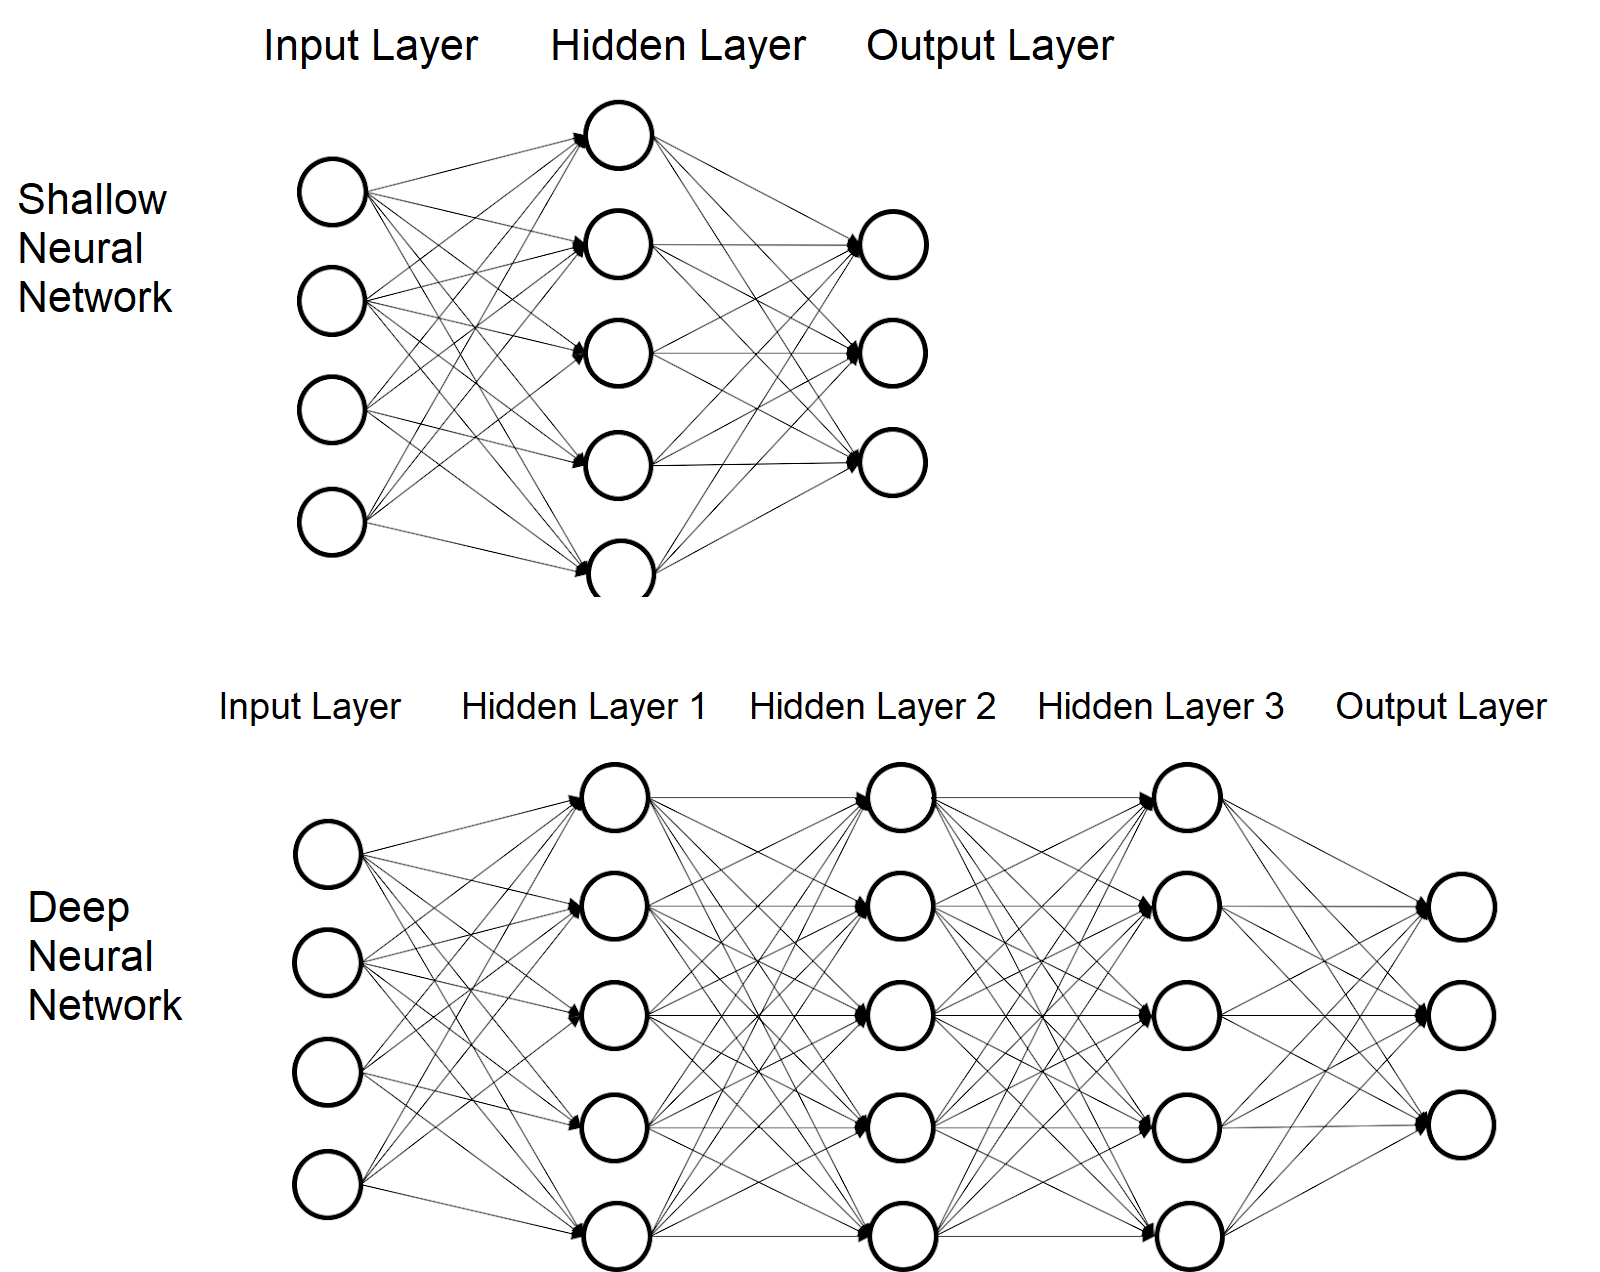
\includegraphics[width=0.7\textwidth]{img/DNN.png}
    \caption{Shallow vs Deep Neural Networks}
    \label{fig:shallow-deep-NN}
\end{figure}

\subsection{Convolutional Neural Networks}
\label{sub:CNN}
This was first proposed by \cite{fukushima_neocognitron_1988} and used by \cite{lecun_gradient-based_1998} for document recognition. It is very popular for image classification but is also used in Speech technology \cite{abdel-hamid_exploring_2013} \cite{ghahremani_acoustic_2016} \cite{dua_developing_2022}. 

CNNs perform better than DNNs due to the fact that they are highly optimised for processing 2D and 3D features like in images and are effective at learning and extracting of 2D features abstractions. Furthermore, CNNs have far fewer parameters than a similarly sized fully connected network. CNNs are made up of feature extractor and classifier modules. Each network layer in the feature extraction module receives the output from the previous layer as its input and passes it on to the next layer \cite{backstrom_introduction_2022}. %The CNN architecture mainly consists of three types of layers: convolution, pooling, and classification.

\begin{figure}[h!]
    \centering
    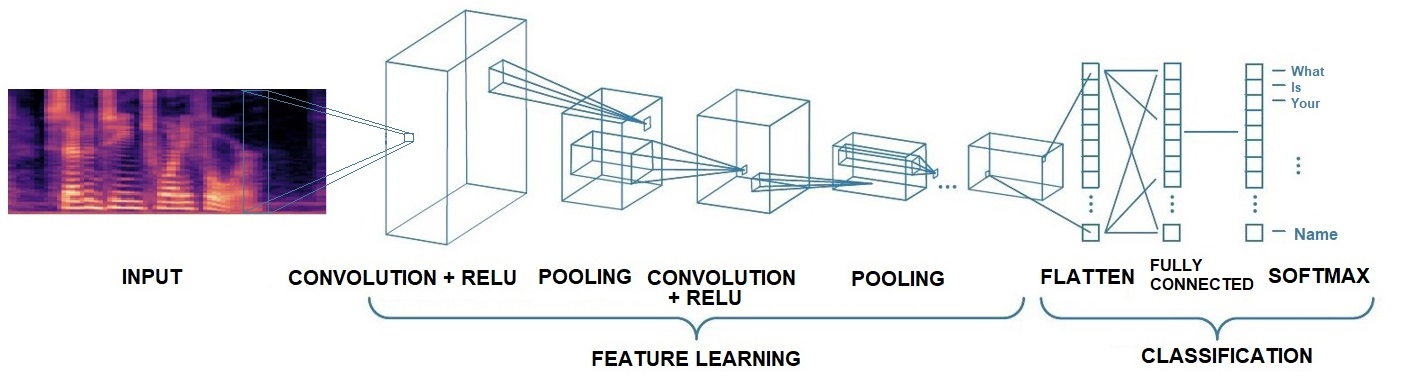
\includegraphics[width=0.95\textwidth]{img/CNN.jpg}
    \caption{CNN Architecture}
    \label{fig:cnn-arch}
\end{figure}

Convolutional Neural Networks consists of mainly following layers \cite{fukushima_neocognitron_1988}:
\begin{enumerate}
    \item \textbf{Convolutional layer:} A filter scans the image a few pixels at a time, to create a feature map predicting the class each feature belongs to. %Thus the feature mappings from previous layers are convolved with learnable kernels in this layer. To form the output feature maps, the kernel output is passed through a linear or non-linear activation function such as sigmoid, hyperbolic tangent, Softmax, rectified linear, and identity functions. Each output feature map can be combined with multiple input feature maps.
    \item \textbf{Pooling layer:} It preserves the most crucial information while reducing the amount of information in each feature obtained from convolution layers. There are typically several convolution and pooling rounds.
    \item \textbf{Fully connected input layer:} It flattens the output of the preceding layers into a single vector that can be used as an input for the following layer.
    \item \textbf{The first fully connected layer:} It applies weights to the feature analysis inputs in order to predict the right label.
    \item \textbf{Fully connected output layer:} Provides the final probabilities for each label.
\end{enumerate}

Higher-level audio features in CNNs are derived from lower-level layer features. As the convolution and pooling operations propagate to the highest layer or level, the dimensions of the features decrease depending on the size of the kernel. To ensure classification accuracy, the number of feature maps typically rises in order to represent the input images' better features. A fully connected network receives its input from the CNN's final layer of output. Since they perform better, feed-forward neural networks are utilised as the classification layer \cite{abdel-hamid_exploring_2013}.

CNNs performance depends on multiple hyper parameters like number of layers, number of feature maps in each layer, the use of dropouts, batch normalization, etc which is why the model must be fine-tuned on the hyper-parameters by conducting multiple experiments to find the right setting of hyper-parameters values after which the model is trained for for a certain given number of epochs \cite{backstrom_introduction_2022}.

\subsection{TDNN}

\begin{figure}[htb]
    \centering
    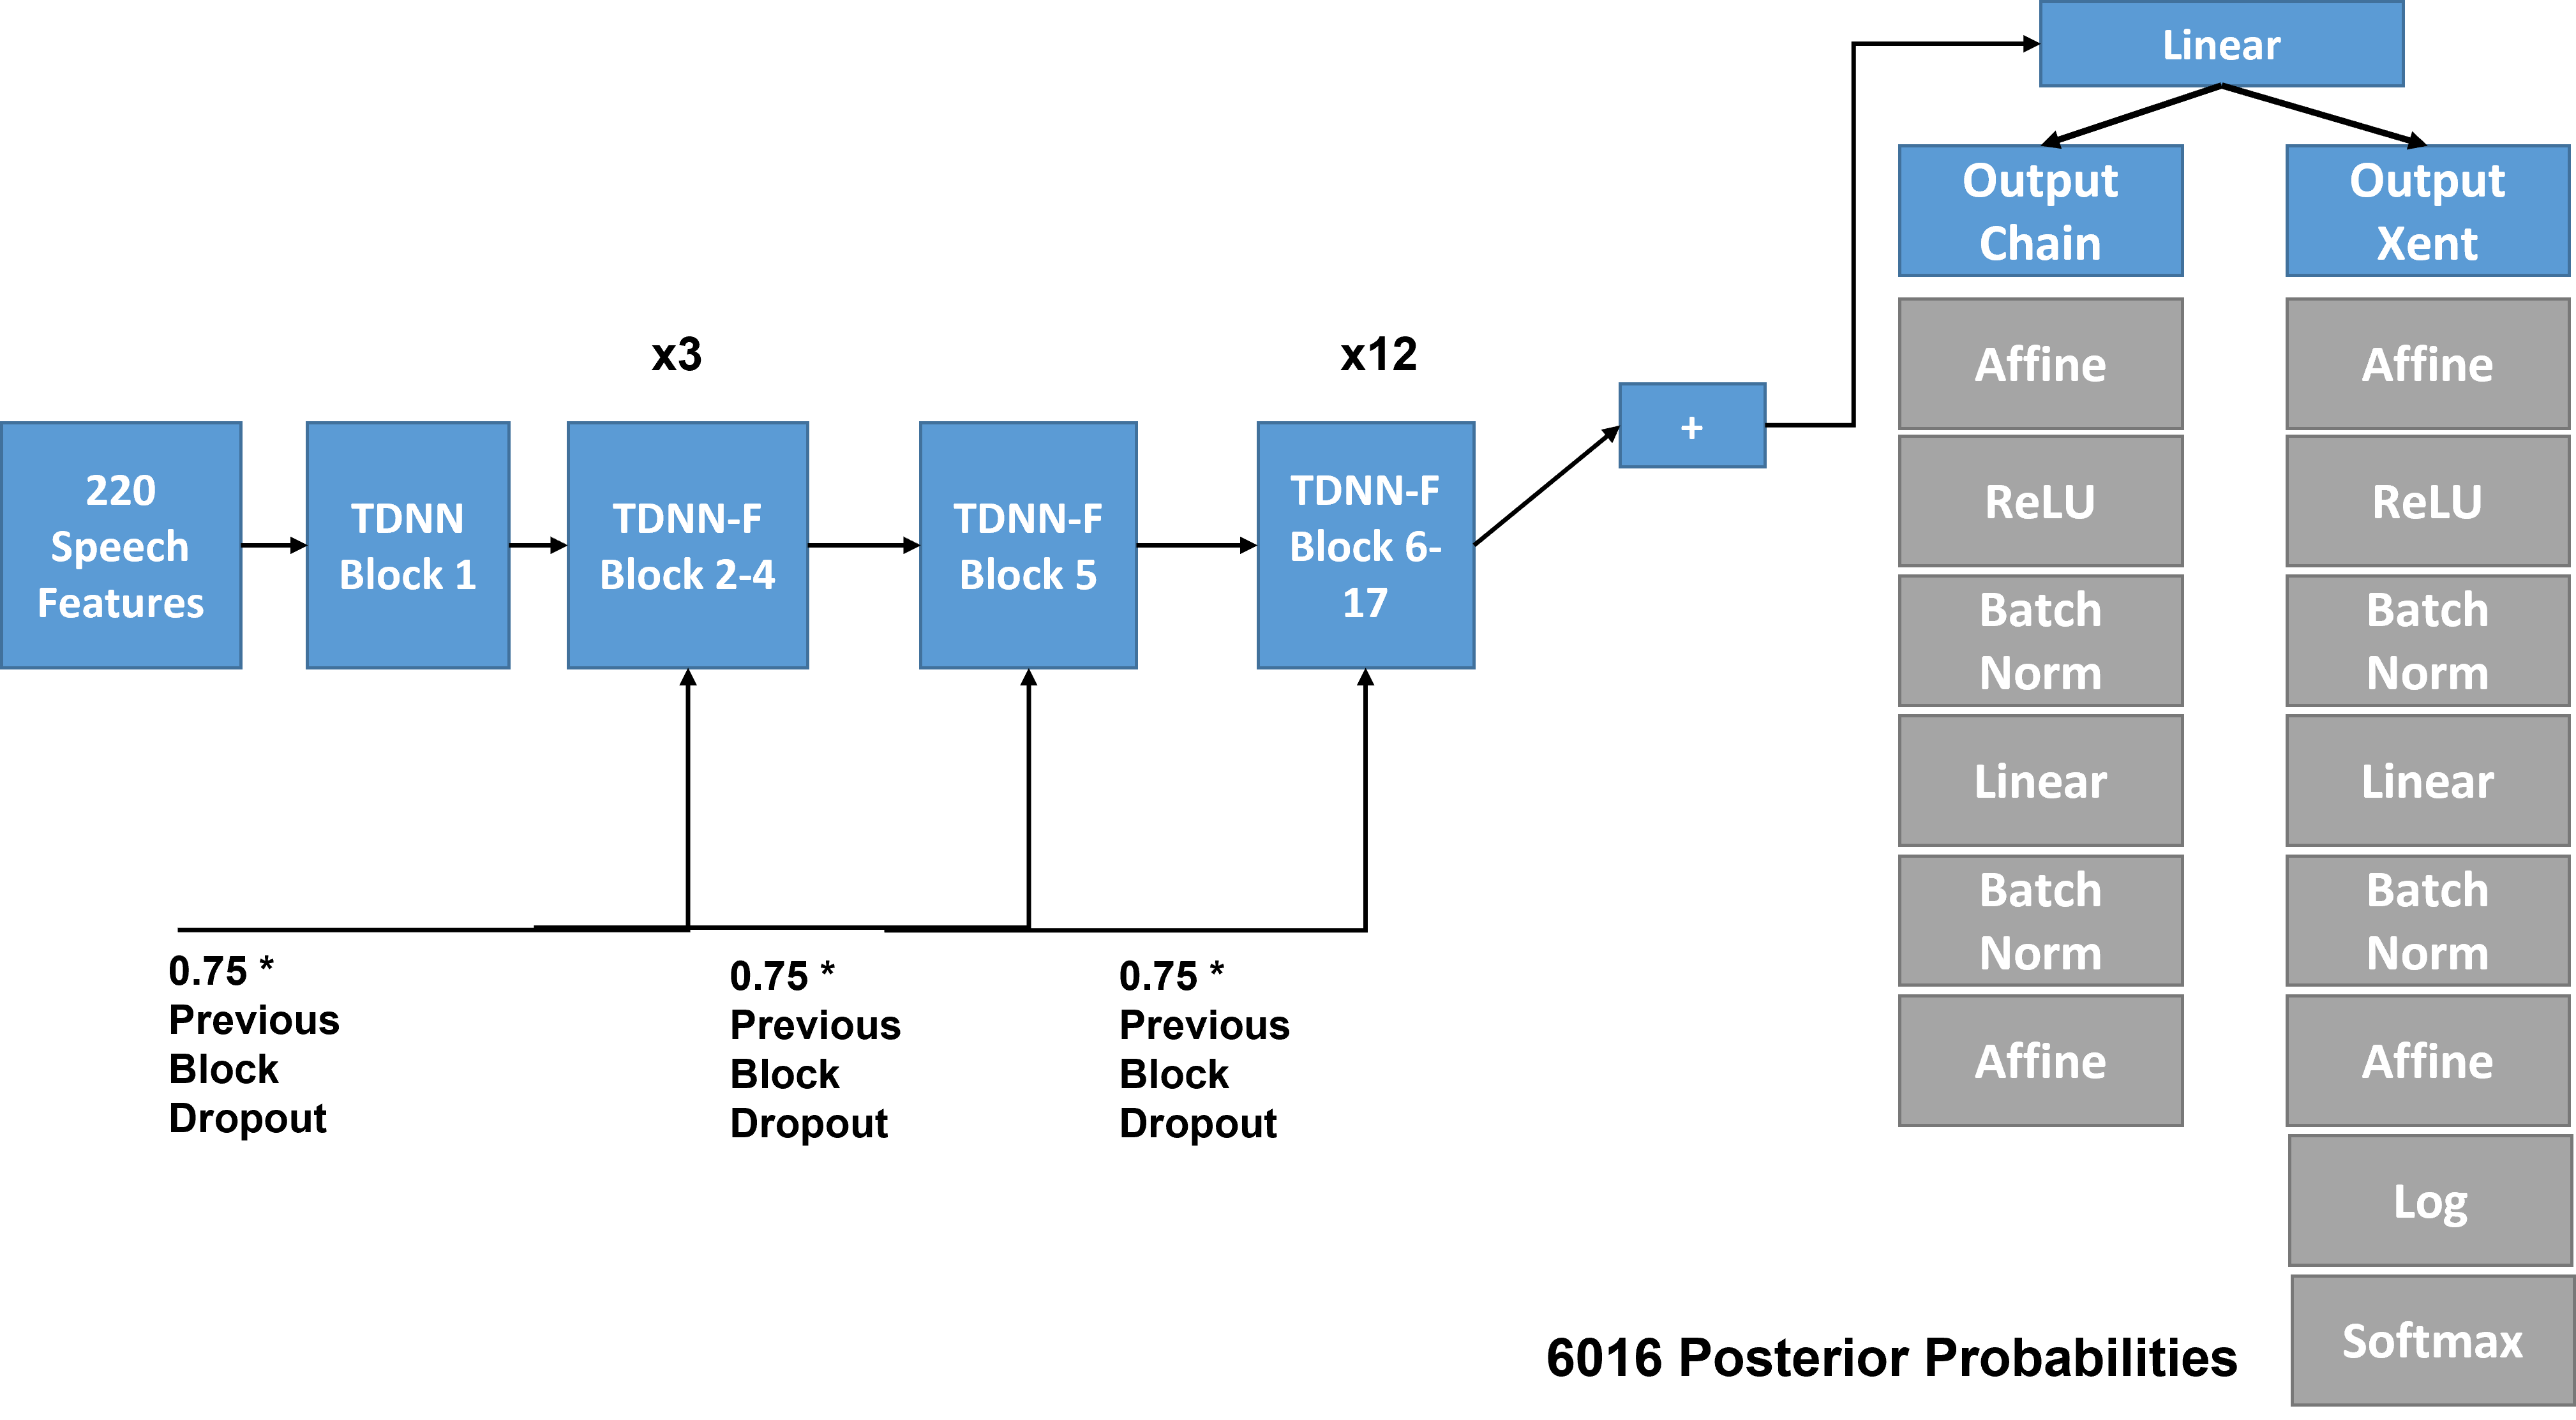
\includegraphics[width=0.9\textwidth]{img/TDNN2.png}
    \caption{TDNN Architecture Basic Layout}
    \label{fig:TDNN-arch}
\end{figure}

Time-Delay Neural Network (TDNN), originally invented by Alex Waibel and Geoffrey Hinton, captures long term temporal correlations between speech frames i.e they are time-dilated 1-Dimensional CNNs. It is a time-domain convolutional network that models temporal dependencies which is easier to parallelize in contrast to a recurrent network and is comparable to feed-forward DNN in terms of training time \cite{noauthor_tdnn_nodate}. It has special characteristics of shift in-variance just like CNN. TDNN can learn short intervals contexts between input features like MFCC and of longer intervals in upper layers i.e. lower layers learn short input contexts, and higher layers learn long input contexts \cite{liu_time_2019}.

\begin{figure}[h!]
    \centering
    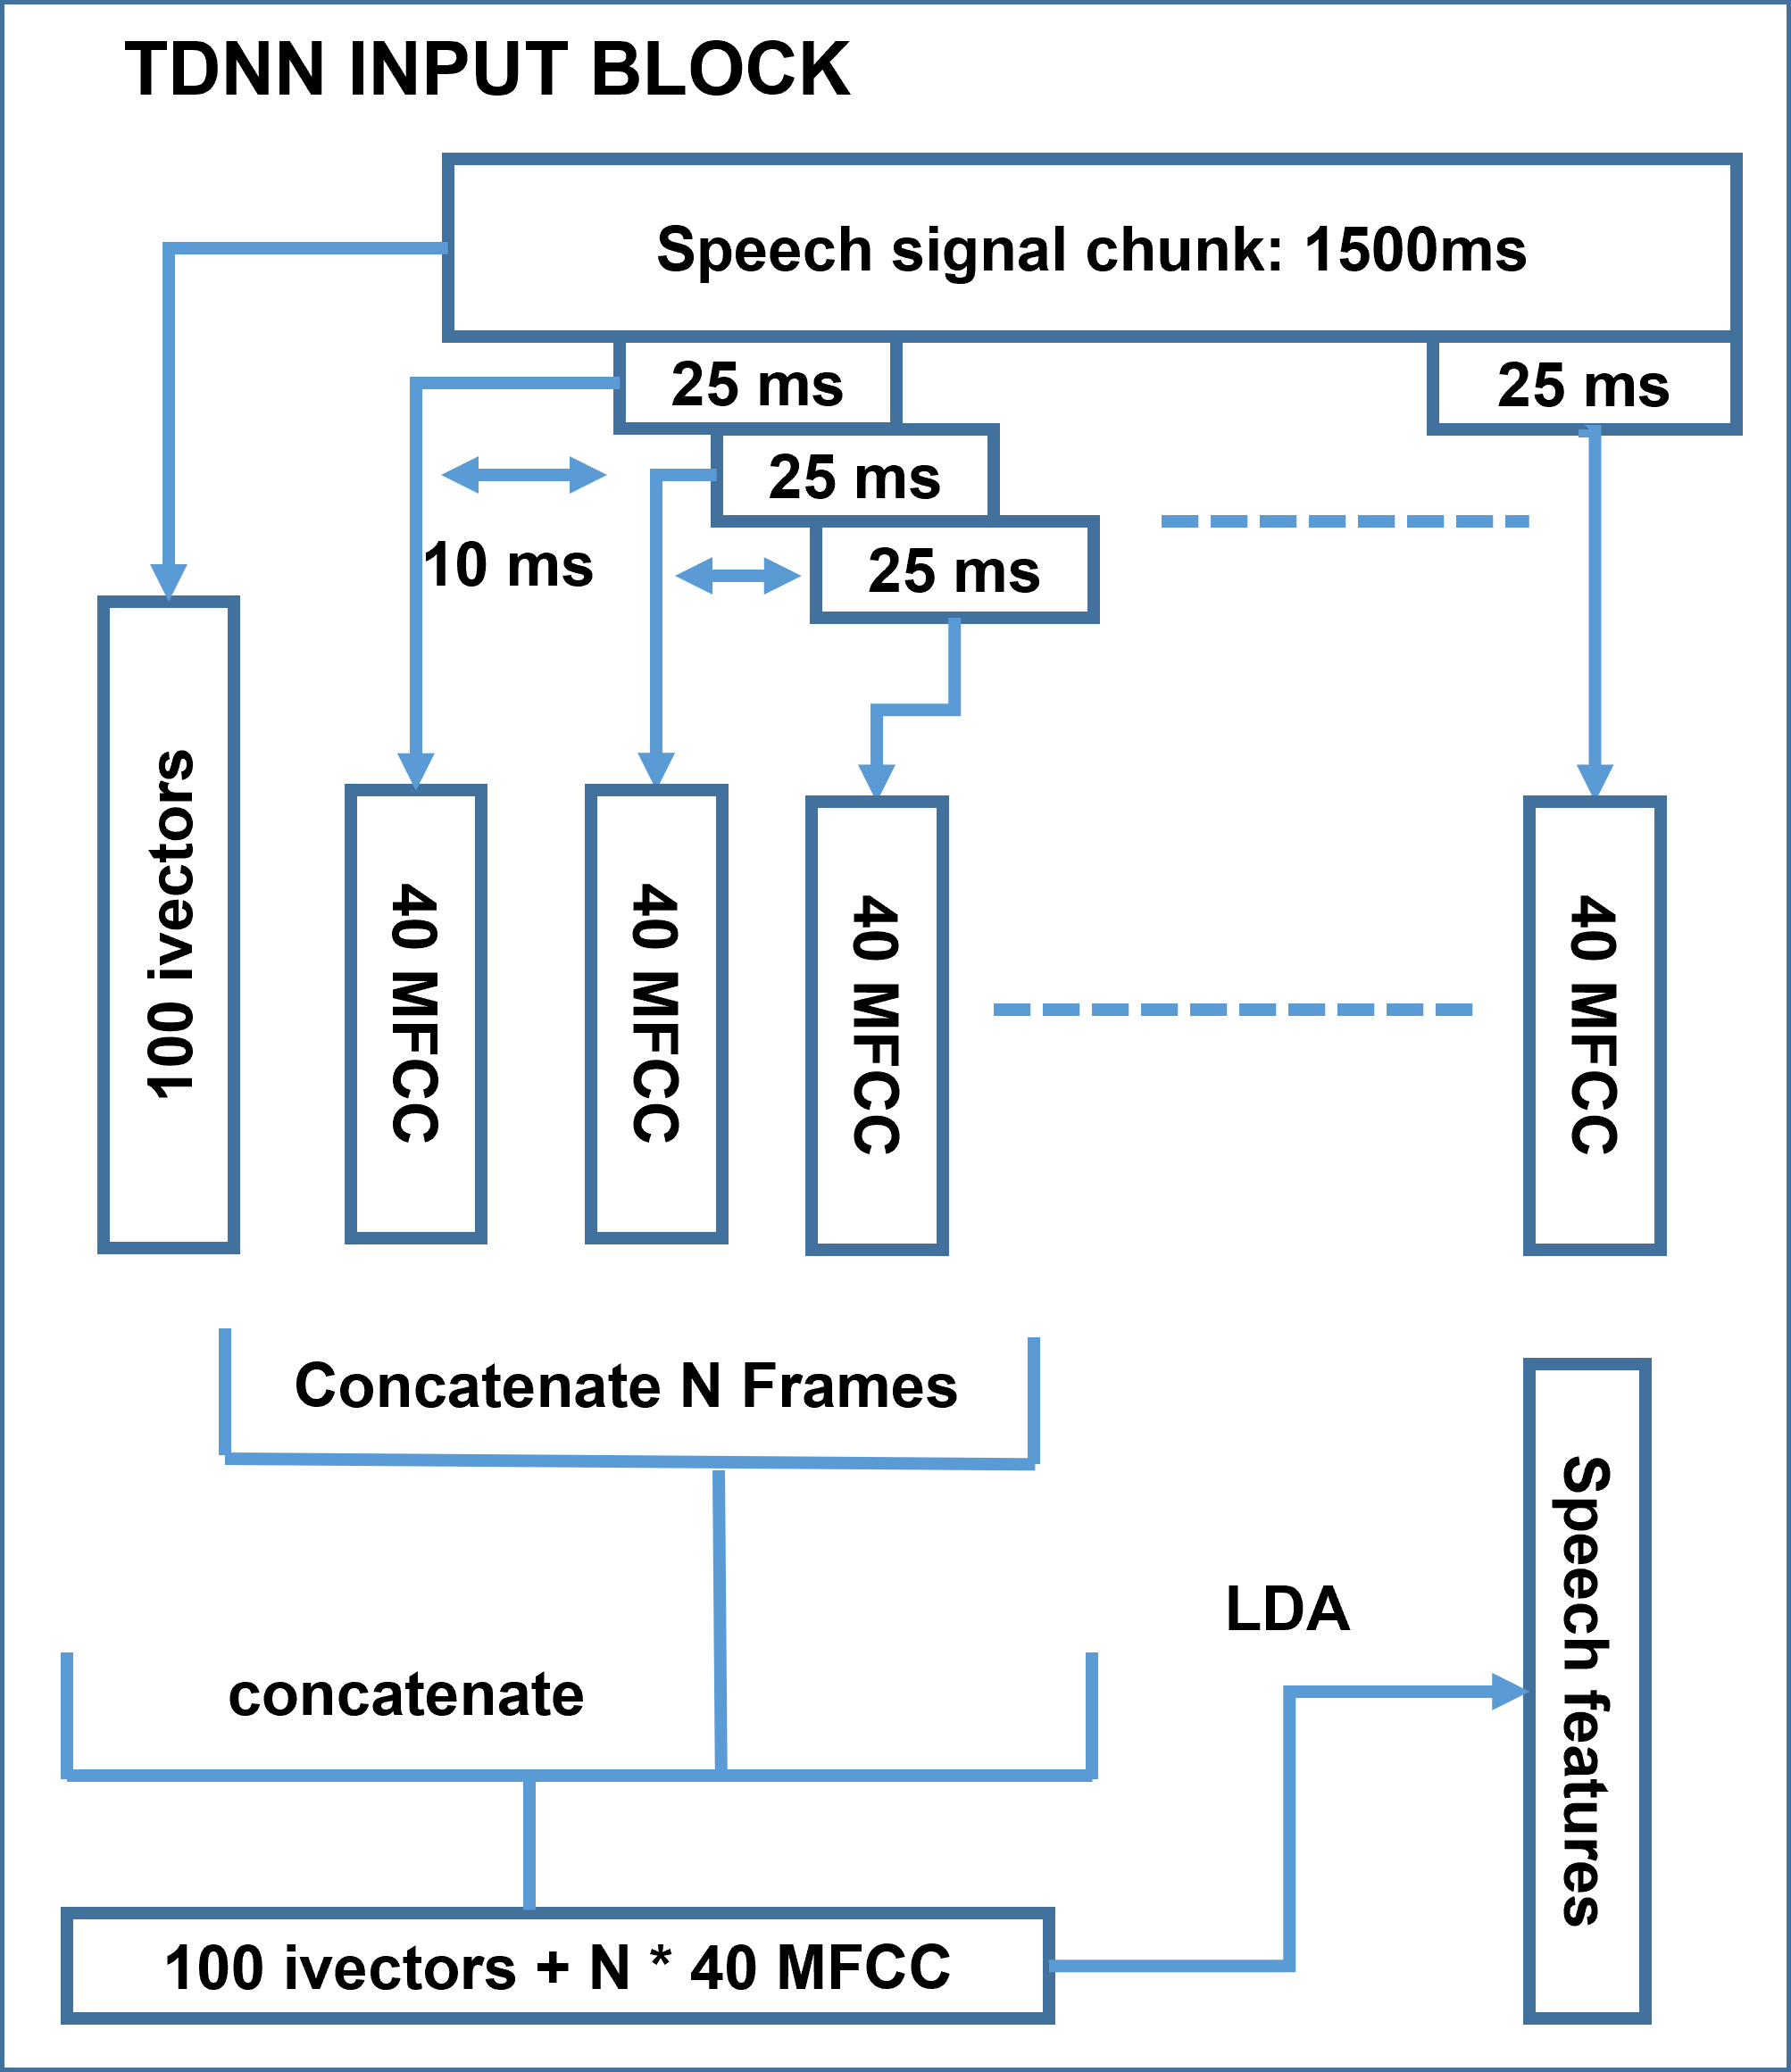
\includegraphics[width=0.4\textwidth]{img/TDNN INPUT.png}
    %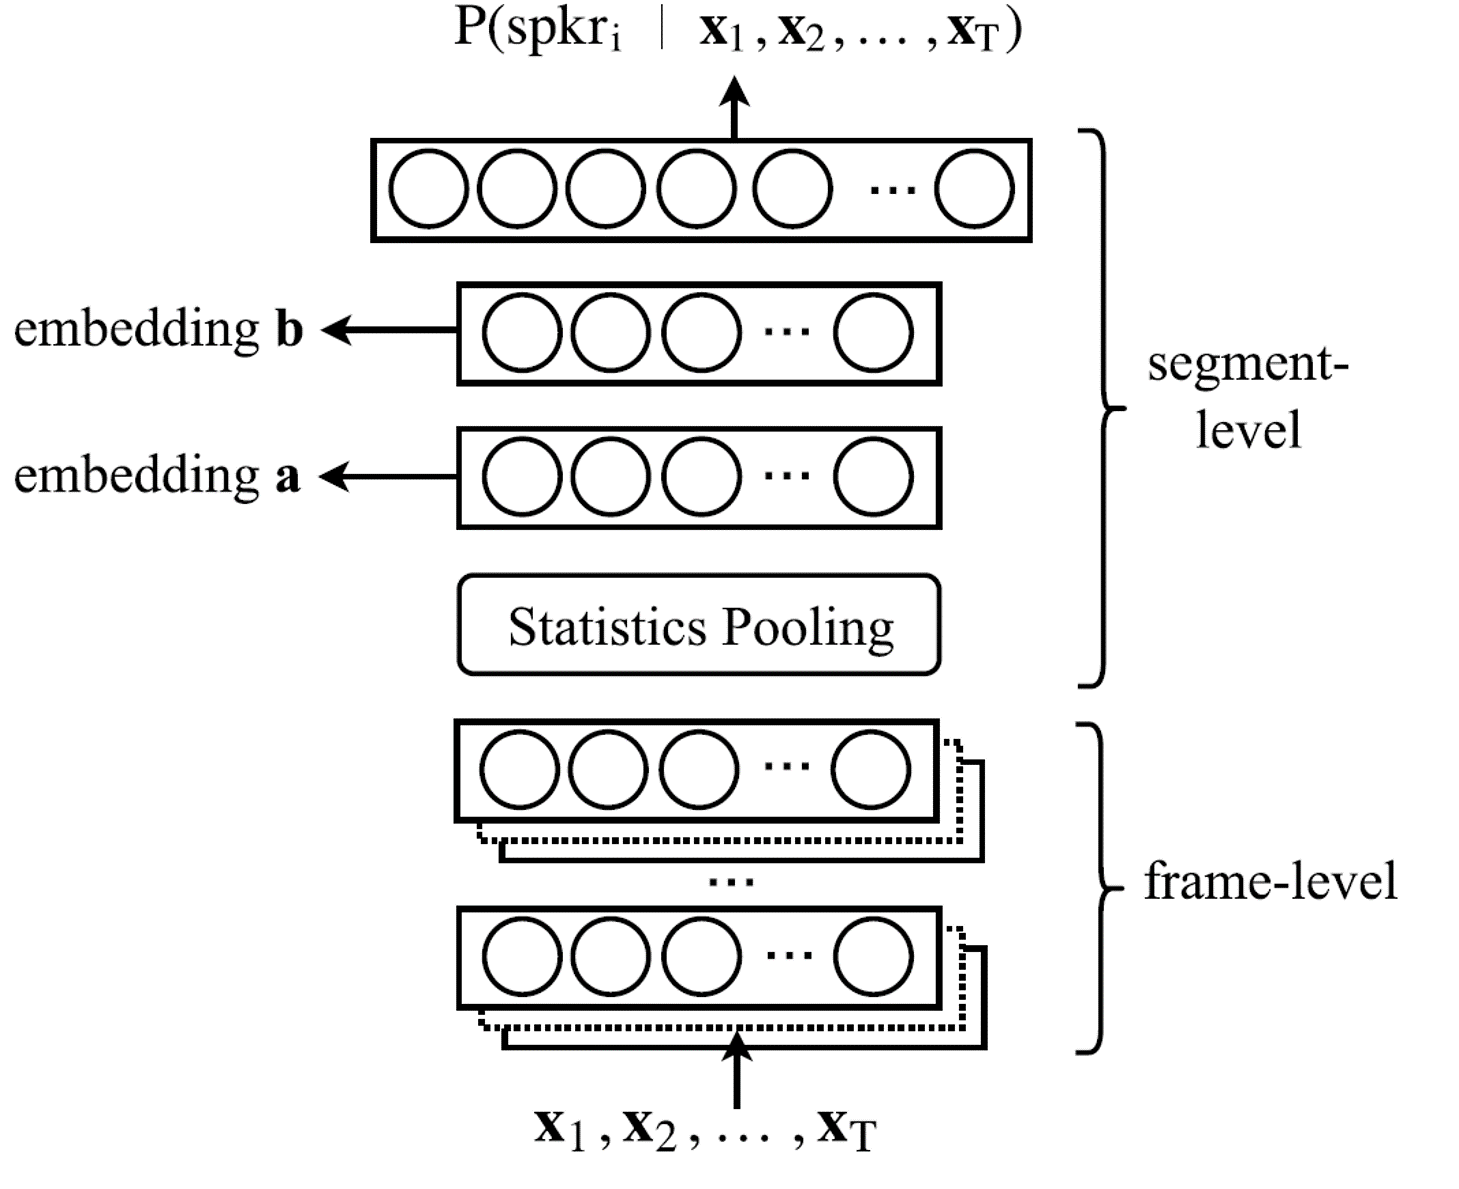
\includegraphics[width=0.4\textwidth]{img/tdDNN frame and segment.png}
    \caption{TDNN Input}   
    \label{fig:TDNN-INPUT}
\end{figure}

Each unit's input is spatially expanded out in a couple of sequential units from the previous TDNN layer. Hence, the lower layers learn a narrow-context and higher layers process a broader temporal-context activations. Each layer's input-context length represents the TDNN hyperparameter \cite{kreyssig_improved_2018}.

All features and frames are correlated in speech. We simply make a 25ms window and take 40 MFCCs of that window or segment. We need previous and next frames to predict next frame in actual. In streaming where we want to predict more on based on past frames instead of future frames, TDNN make better sense \cite{liu_time_2019}. 

\begin{figure}[h!]
    \centering
    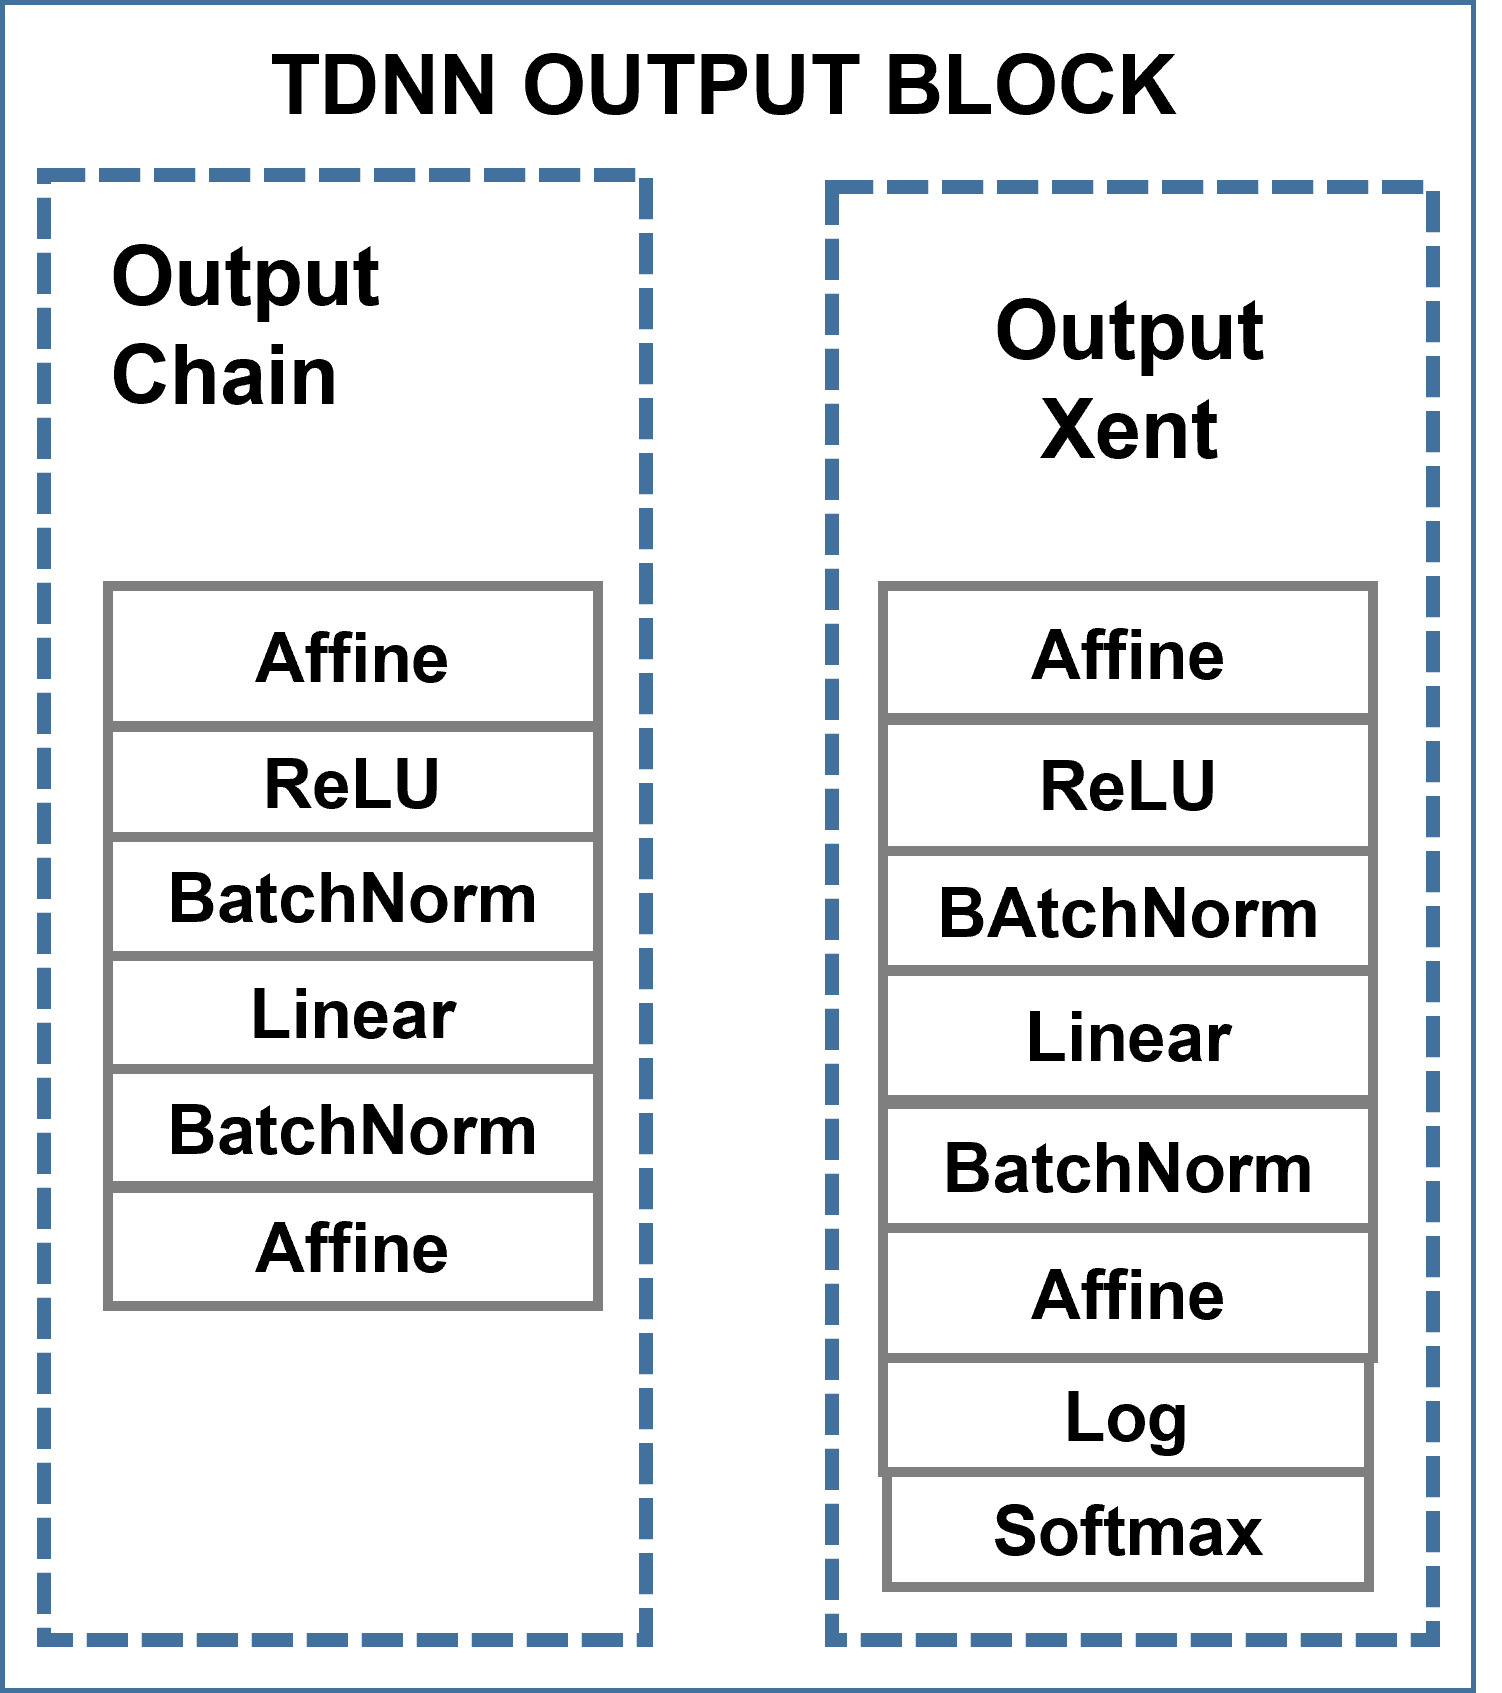
\includegraphics[width=0.3\textwidth]{img/TDNNOUTPUT.png}
    \caption{TDNN Output Block}
    \label{fig:TDNN-OUTPUT-BLOC}
\end{figure}

%\begin{figure}[h!]
%    \centering
%    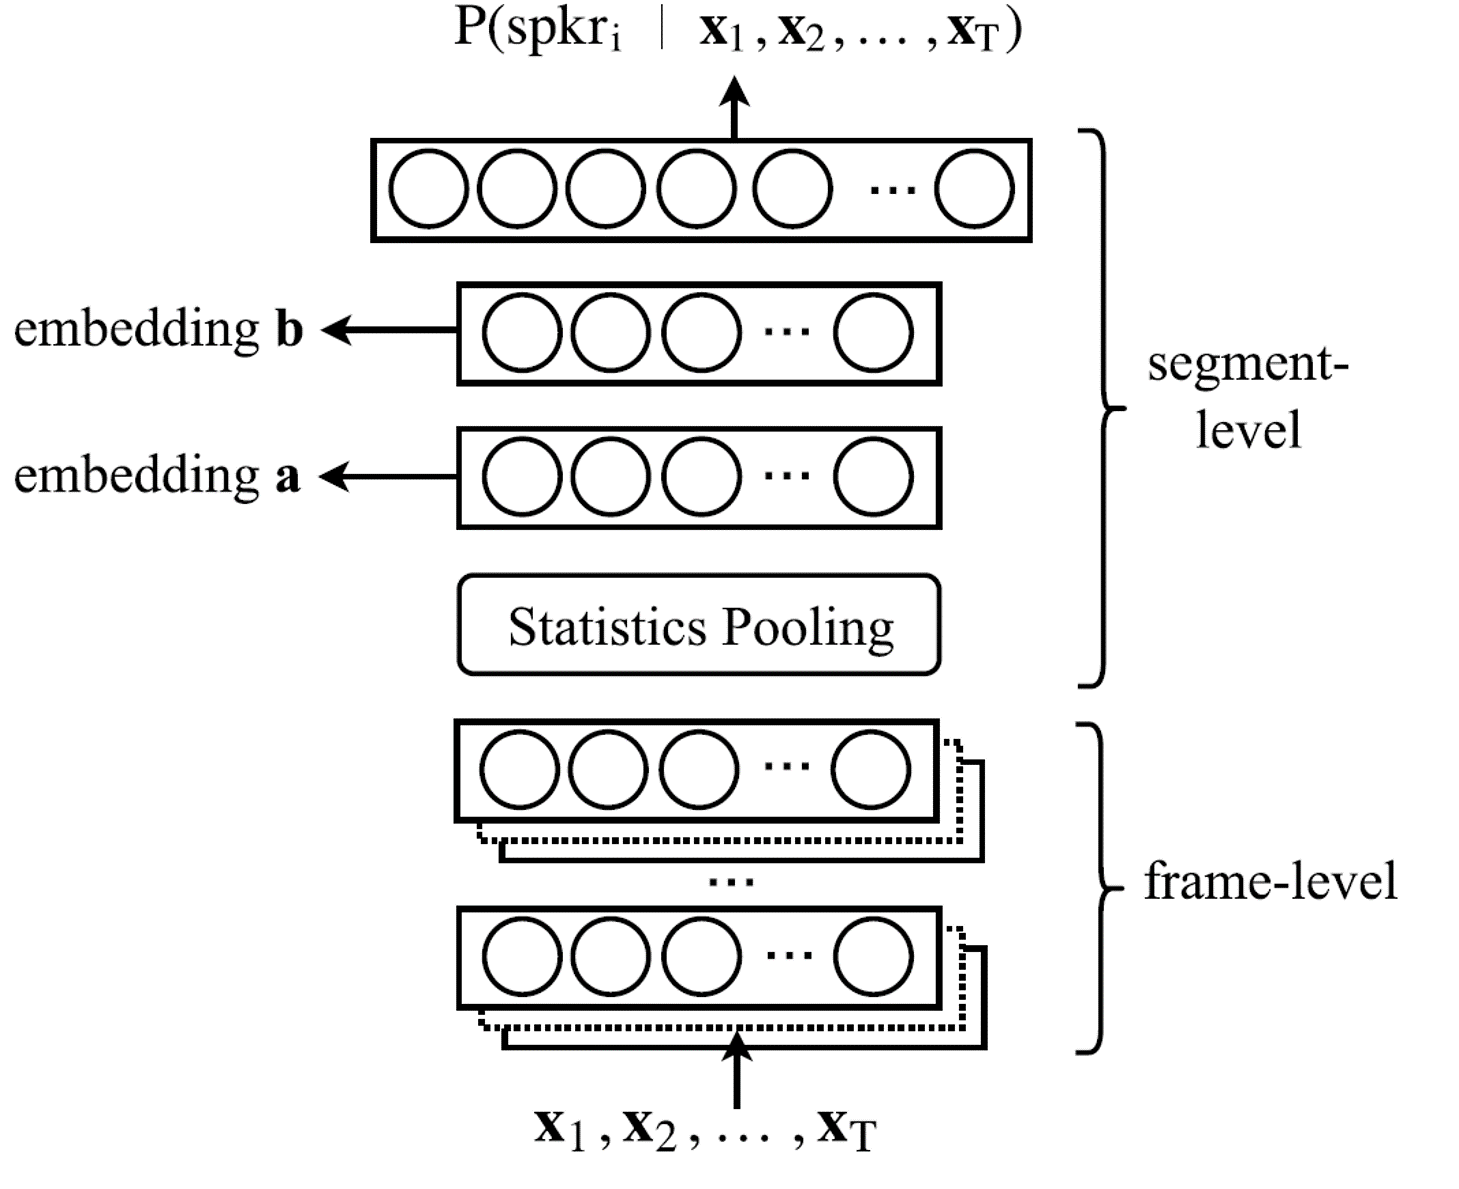
\includegraphics[width=0.5\textwidth]{img/tdDNN frame and segment.png}
%    \caption{TDNN Layers at frame and segment level}
%    \label{fig:TDNN Layers}
%\end{figure}

Input patches consist of fixed number of feature vectors as input to which processes them with fixed local temporal context. The context width increases as we go to upper layers. Finally the last layer representation is pooled by statistics pool layer. The network consist of TDNN which operates at frame level. The last layer output representations from TDNN goes to Statistics pooling layer at every time step. Statistic pool layer computes mean and standard vectors for all the representations from frame 1 to T. Finally these pooled representation goes to next layer which applies affine transformation followed by softmax which can be used for Speech to text of identifying speakers \cite{liu_time_2019}. 

The TDNN architecture is learned on narrow contexts and the upper layers of the networks process wider contexts of the input features, whereas the general Feed Forward Neural Network learns entire input features for processing contexts. Each TDNN layer is updated by a different resolution, which increases as the network layers. By removing duplicated weights from the networks, the TDNN is optimised. A standard Feed Forward Neural learns overlapping features, and removing these duplicated updates reduces training time \cite{yeh_taiwanese_2020}. 

A subsampling is used to reduce duplicated inputs as shown in \ref{fig:tdnn-subsampling} in which nodes and weights (shown by dashed line) are updated only upon application of sub-sampling. The technique does not connect multiple inputs in a hidden layer by allowing space between frames. Since TDNN has a long context going up to the upper layer, the model can learn all input features if the interval between frames is allowed \cite{ritter_neural_2019}. 

\begin{figure}[h!]
    \centering
    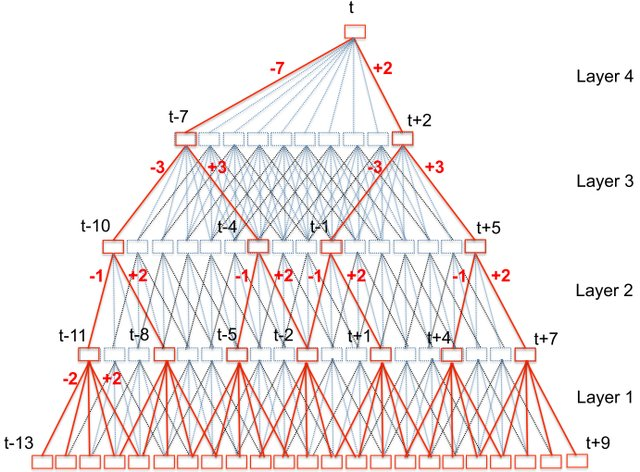
\includegraphics[width=0.8\textwidth]{img/Tdnn-subsampling.jpg}
    \caption{TDNN subsampling \cite{ritter_neural_2019}}
    \label{fig:tdnn-subsampling}
\end{figure}

Furthermore, minimizing the number of edges and nodes in the network reduces the number of parameters that represent the model. Long-term temporal dependencies are better captured by TDNN architecture than by feed-forward DNN. In comparison to baseline DNN model in interactive personal assistant (IPA) domain there is a relative improvement of 7.3\%.  The TDNN is also used to remove reverberation effects in robust acoustic modelling. Using iVectors as input helps TDNN to perform instantaneous speaker and environment adaptation potentially improving 10\% WER \cite{yeh_taiwanese_2020}.

Increasing TDNN layers enables the network to capture features for a longer time period. Deepening the number of network layers of TDNN helps yield better results. However, deeper network tends to cause degradation, hence, the increasing depth of the neural network reduces accuracy for which a different TDNN architecture is used  in order to achieve better speech recognition performance in which Matrix Factorization training of the network makes neural network training stable \cite{povey_semi-orthogonal_2018}.

\subsection{CNN-TDNN}

CNN-TDNN \cite{ghahremani_acoustic_2016} is a variant of simple TDNN model and it is part of a multi-component system comprising of a hybrid HMM-TDNN based acoustic, phonetic and n-gram language model. It has CNN blocks before the TDNN blocks and takes Mel Filterbanks as input instead of MFCCs. The detailed working of CNN-TDNN is given in Section \ref{sec:LFMMI-chain}.

\begin{figure}[htb]
    \centering
    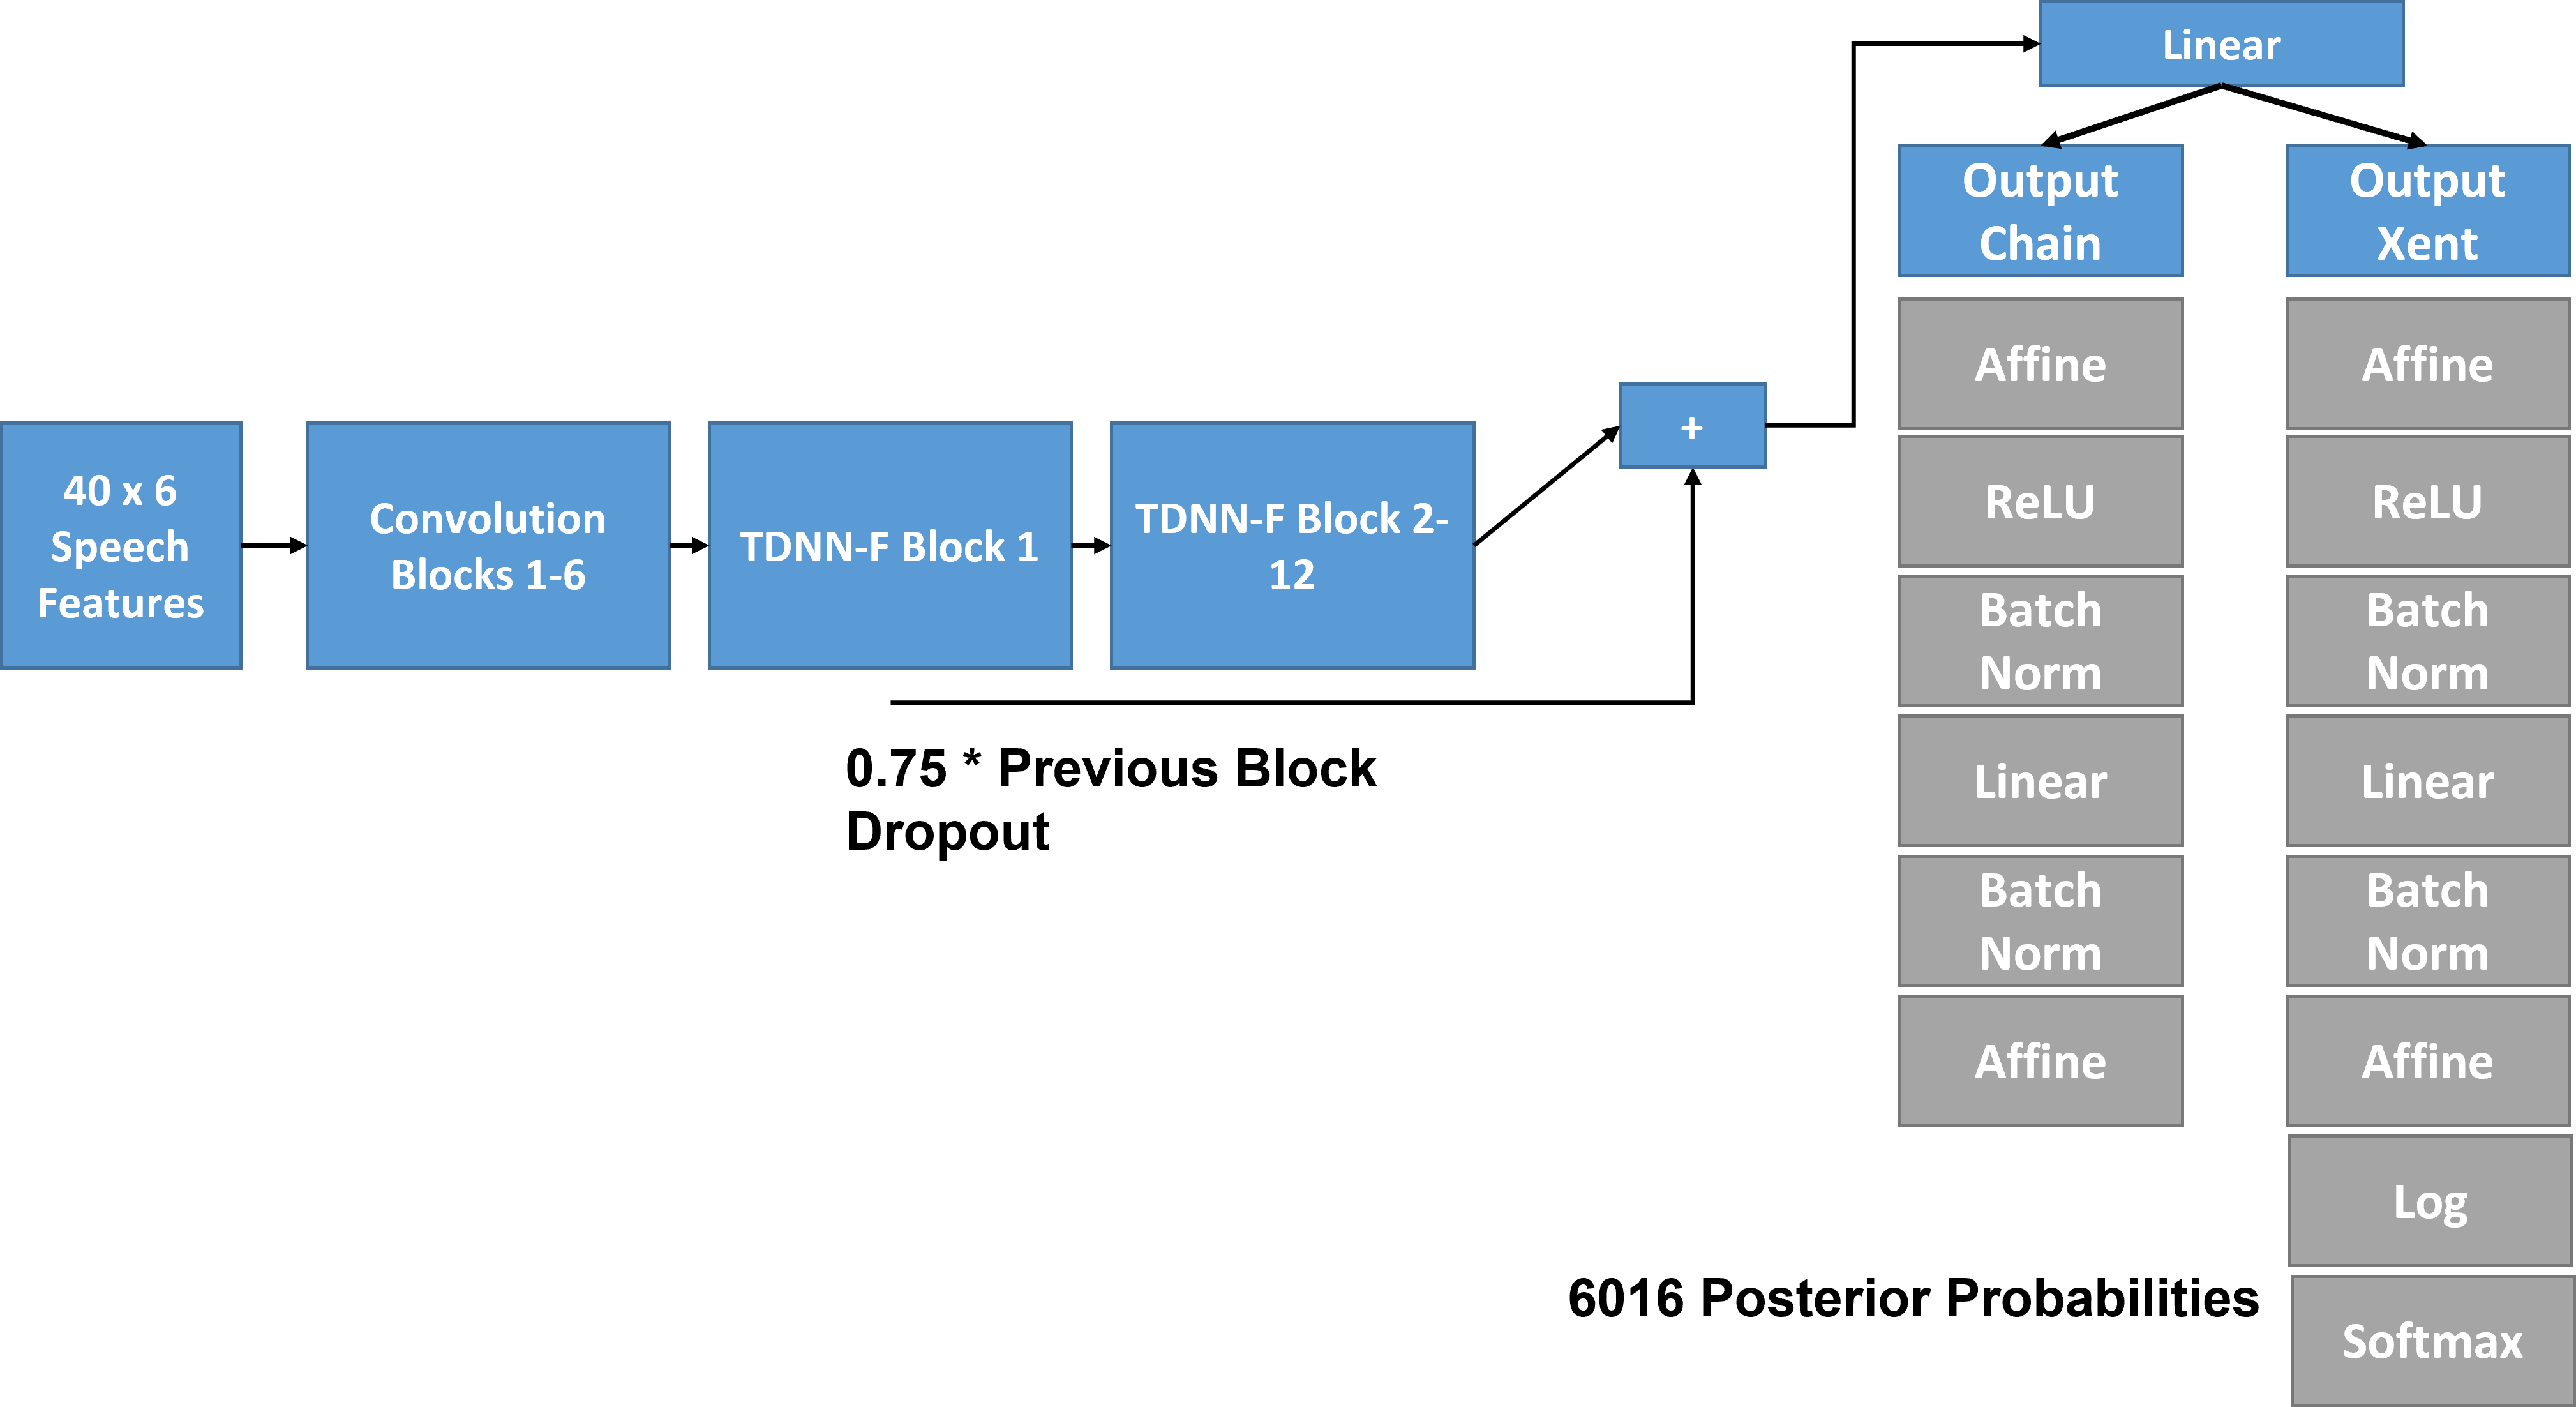
\includegraphics[width=0.7\textwidth]{img/CNNTDNN2.png}
    \caption{CNN-TDNN Basic Layout}
    \label{fig:CNNTDNN-Layout}
\end{figure}

\begin{figure}[h!]
    \centering
    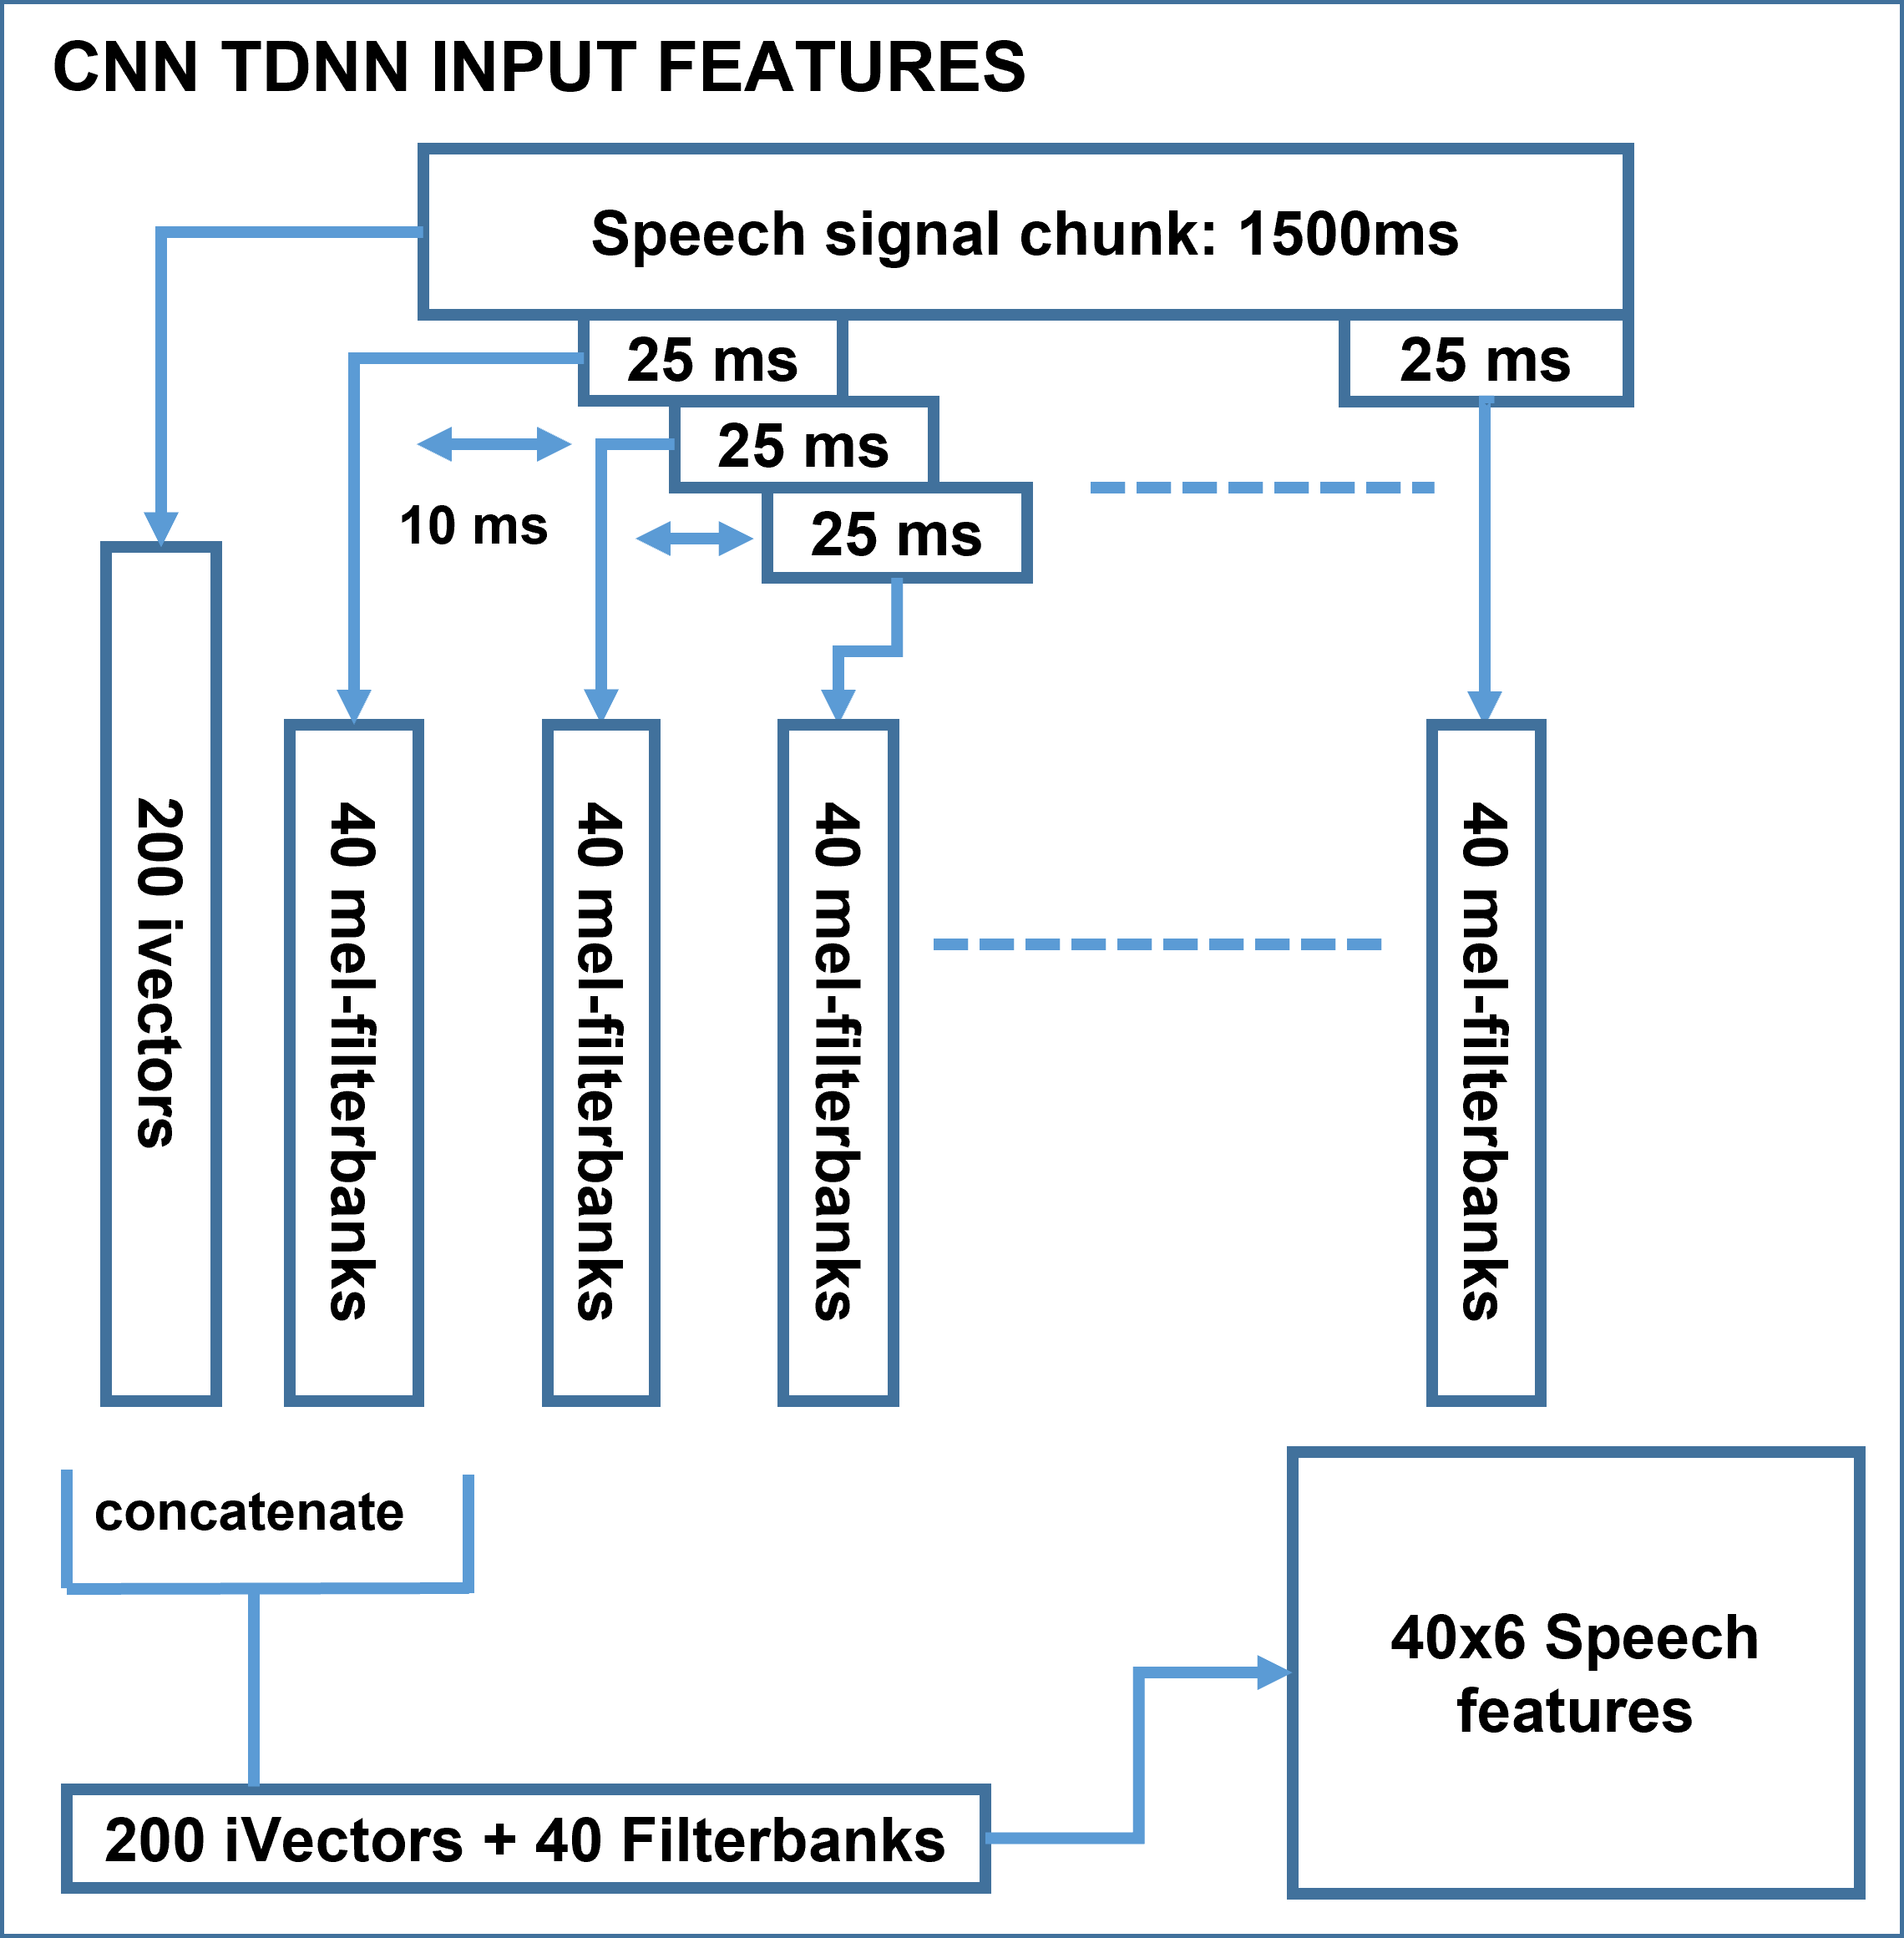
\includegraphics[width=0.4\textwidth]{img/CNNTDNN-INPUT.png}
    \caption{CNN-TDNN Input}
    \label{fig:CNN-TDNN-INPUT}
\end{figure}



\begin{figure}[h!]
    \centering
    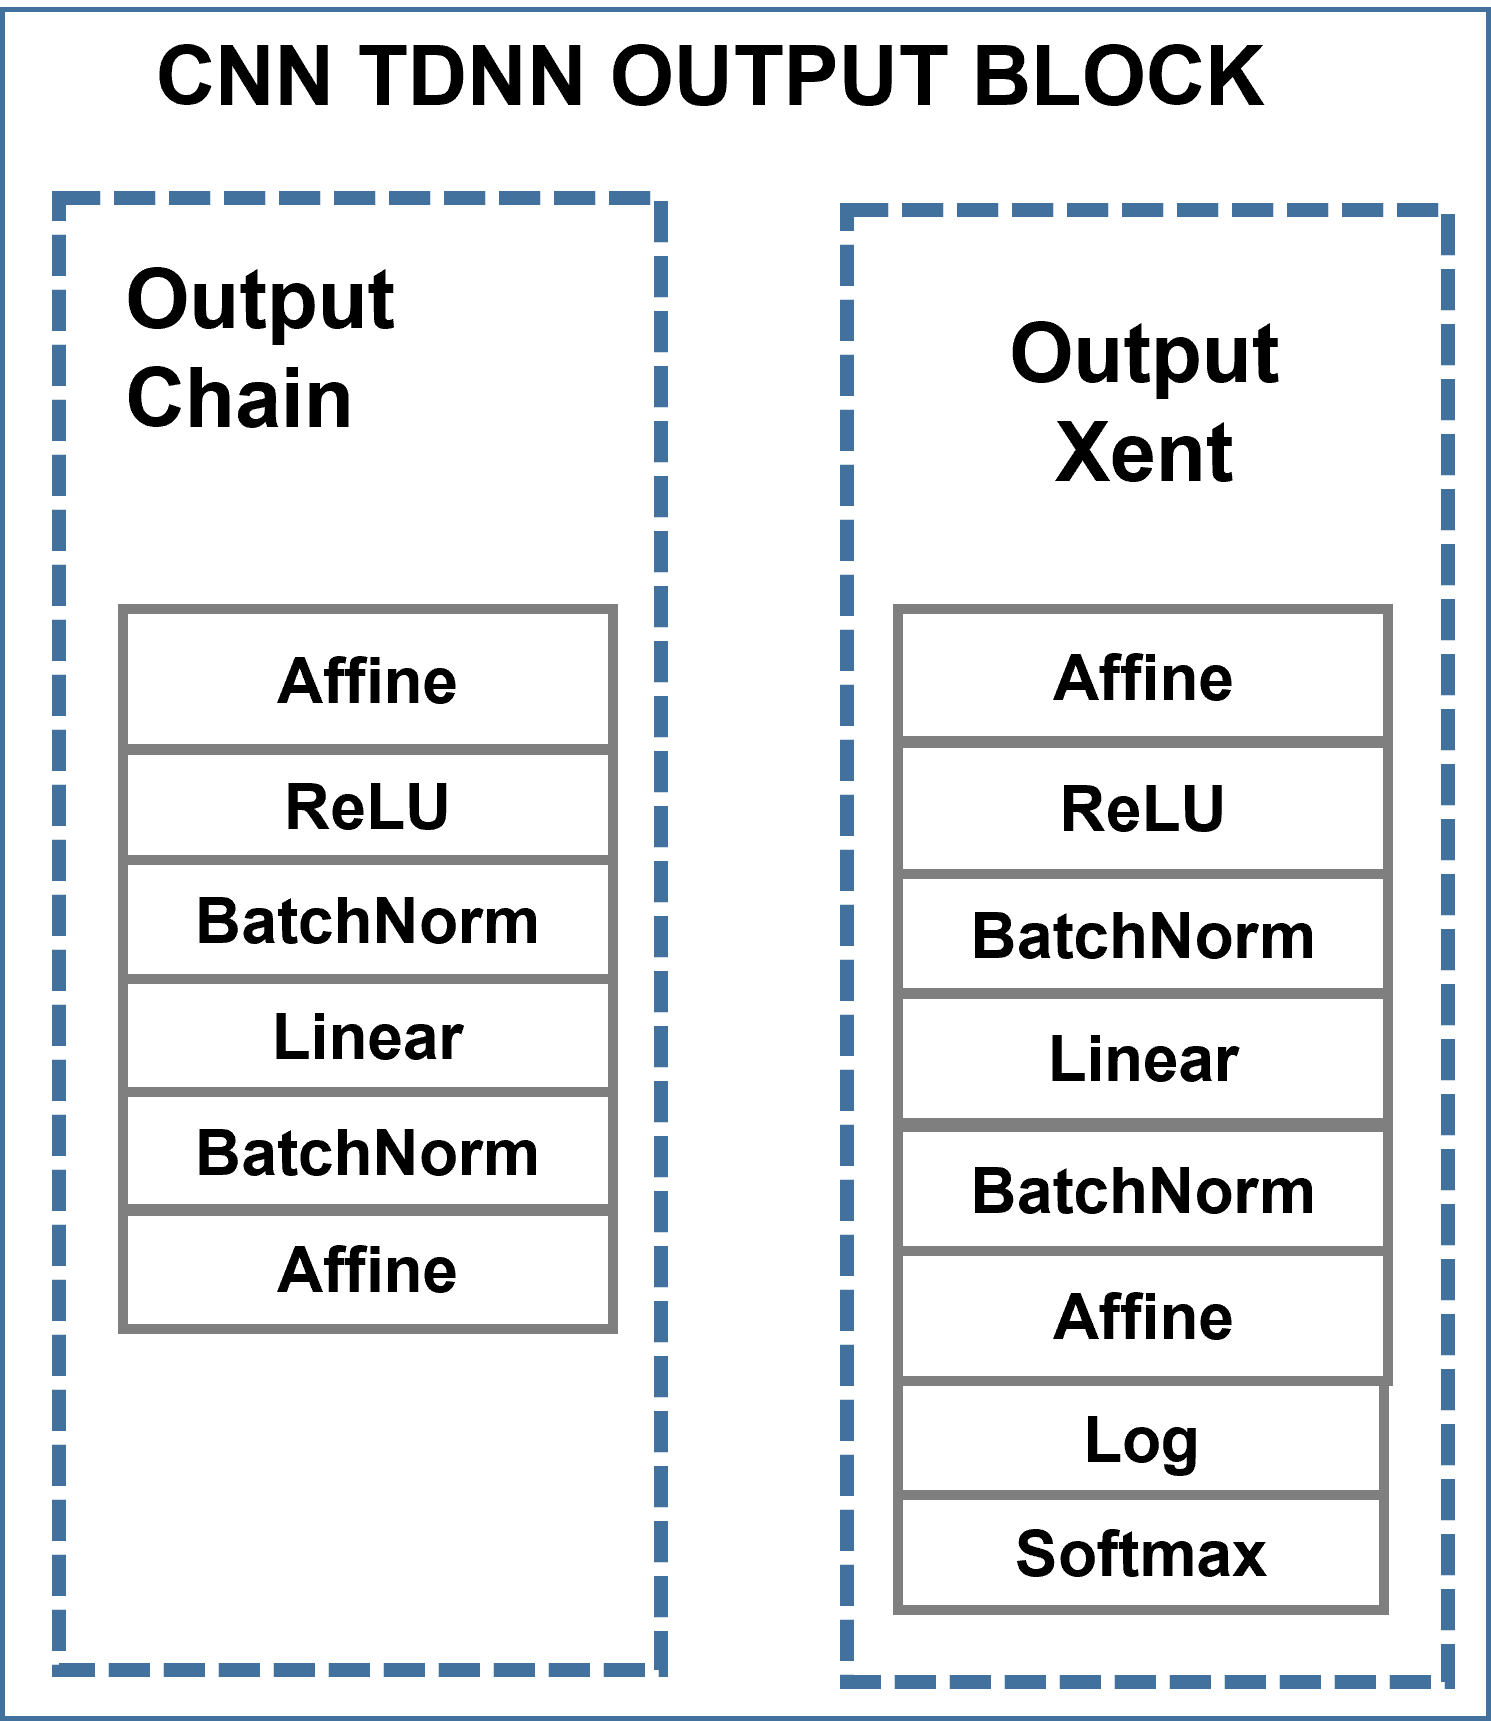
\includegraphics[width=0.4\textwidth]{img/CNNTDNNOUTPUT.png}
    \caption{CNN-TDNN Output}
    \label{fig:CNNTDNN-output}
\end{figure}

%Ghahremani \cite{ghahremani_acoustic_2016} proposed a CNN-TDNN-based raw waveform setup with a repeated network-in-network structure that aggregates time information from convolution filter outputs.

%It introduces Network in Network layer which is a group of micro neural network blocks applied to non-overlapping patches of input with each block being a nonlinear transformation from m dimensional space to n-dimensional space. NIN is a many-to-many non-linearity comprising of two block diagonal matrices, with repeated blocks, inter-leaved between layers of ReLU or Rectified Linear Units. To stabilize training we always add a normalization layer after the NIN non-linearity.

%If the micro neural network block parameters are shared across the NIN, each column of the block $U_{1}$ can be interpreted as a one dimension convolution filter with a filter size \textit{m} and a filter shift \textit{m}. Thus, the same filter is applied to non-overlapping patches and this models local connectivity. The shared parameters in the NIN non-linearity keeps its total parameter count low relative to the size of its input and output, and allows it to be trained faster \cite{ghahremani_acoustic_2016}.

%\begin{figure}[h]
%    \centering
%    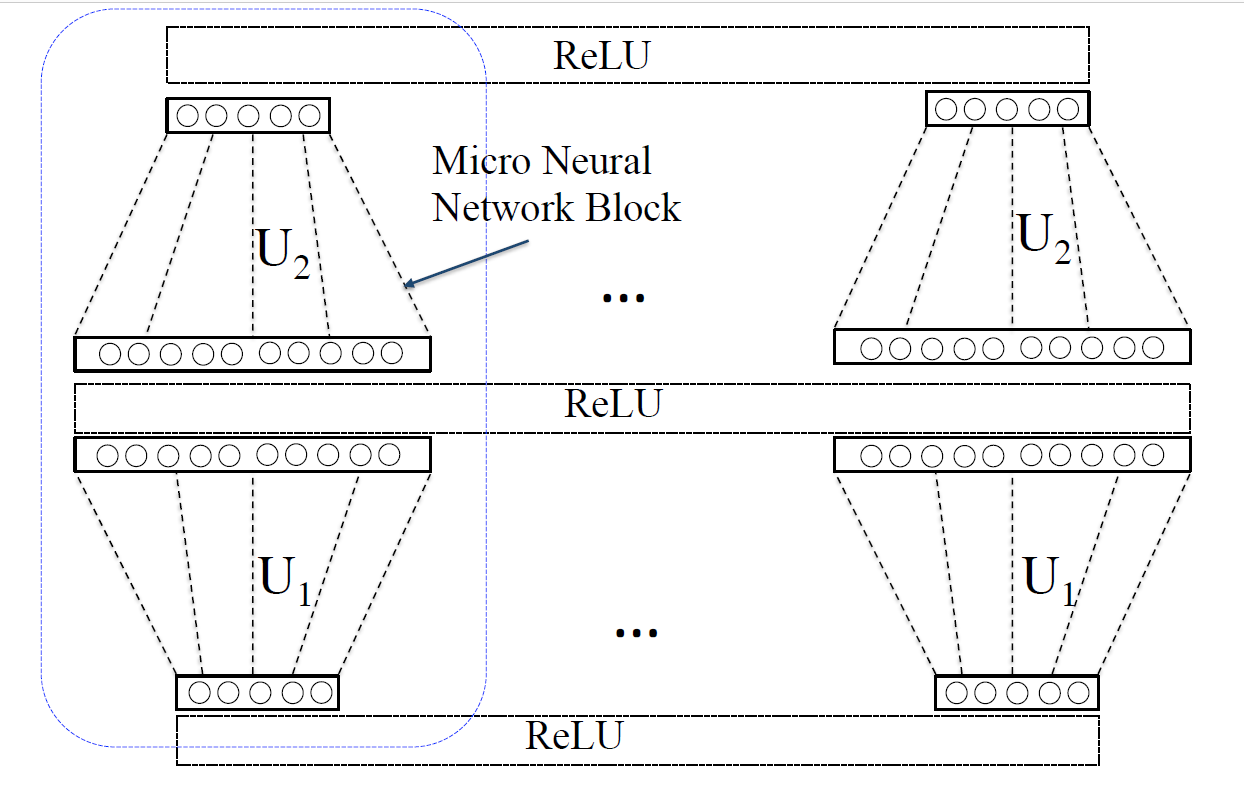
\includegraphics[width=0.6\textwidth]{img/NIN.png}
%    \caption{NIN structure}
%    \label{fig:NIN}
%\end{figure}

%If this Network In Network (NIN) non-linearity replaces the conventional ReLU hidden layer in the DNN, the results improve. 

\section{Training ASRs Completely on Deep Neural Networks}

Due of the shortcomings of the Statistical HMM-based model and coupled with the promotion of deep learning technology, more and more works began to study end-to-end LVCSR. The goal was to bypass the complex structuring of Traditional ASR to achieve a joint language and acoustic model of sorts in one model using Deep Learning.

\begin{figure}[h]
    \centering
    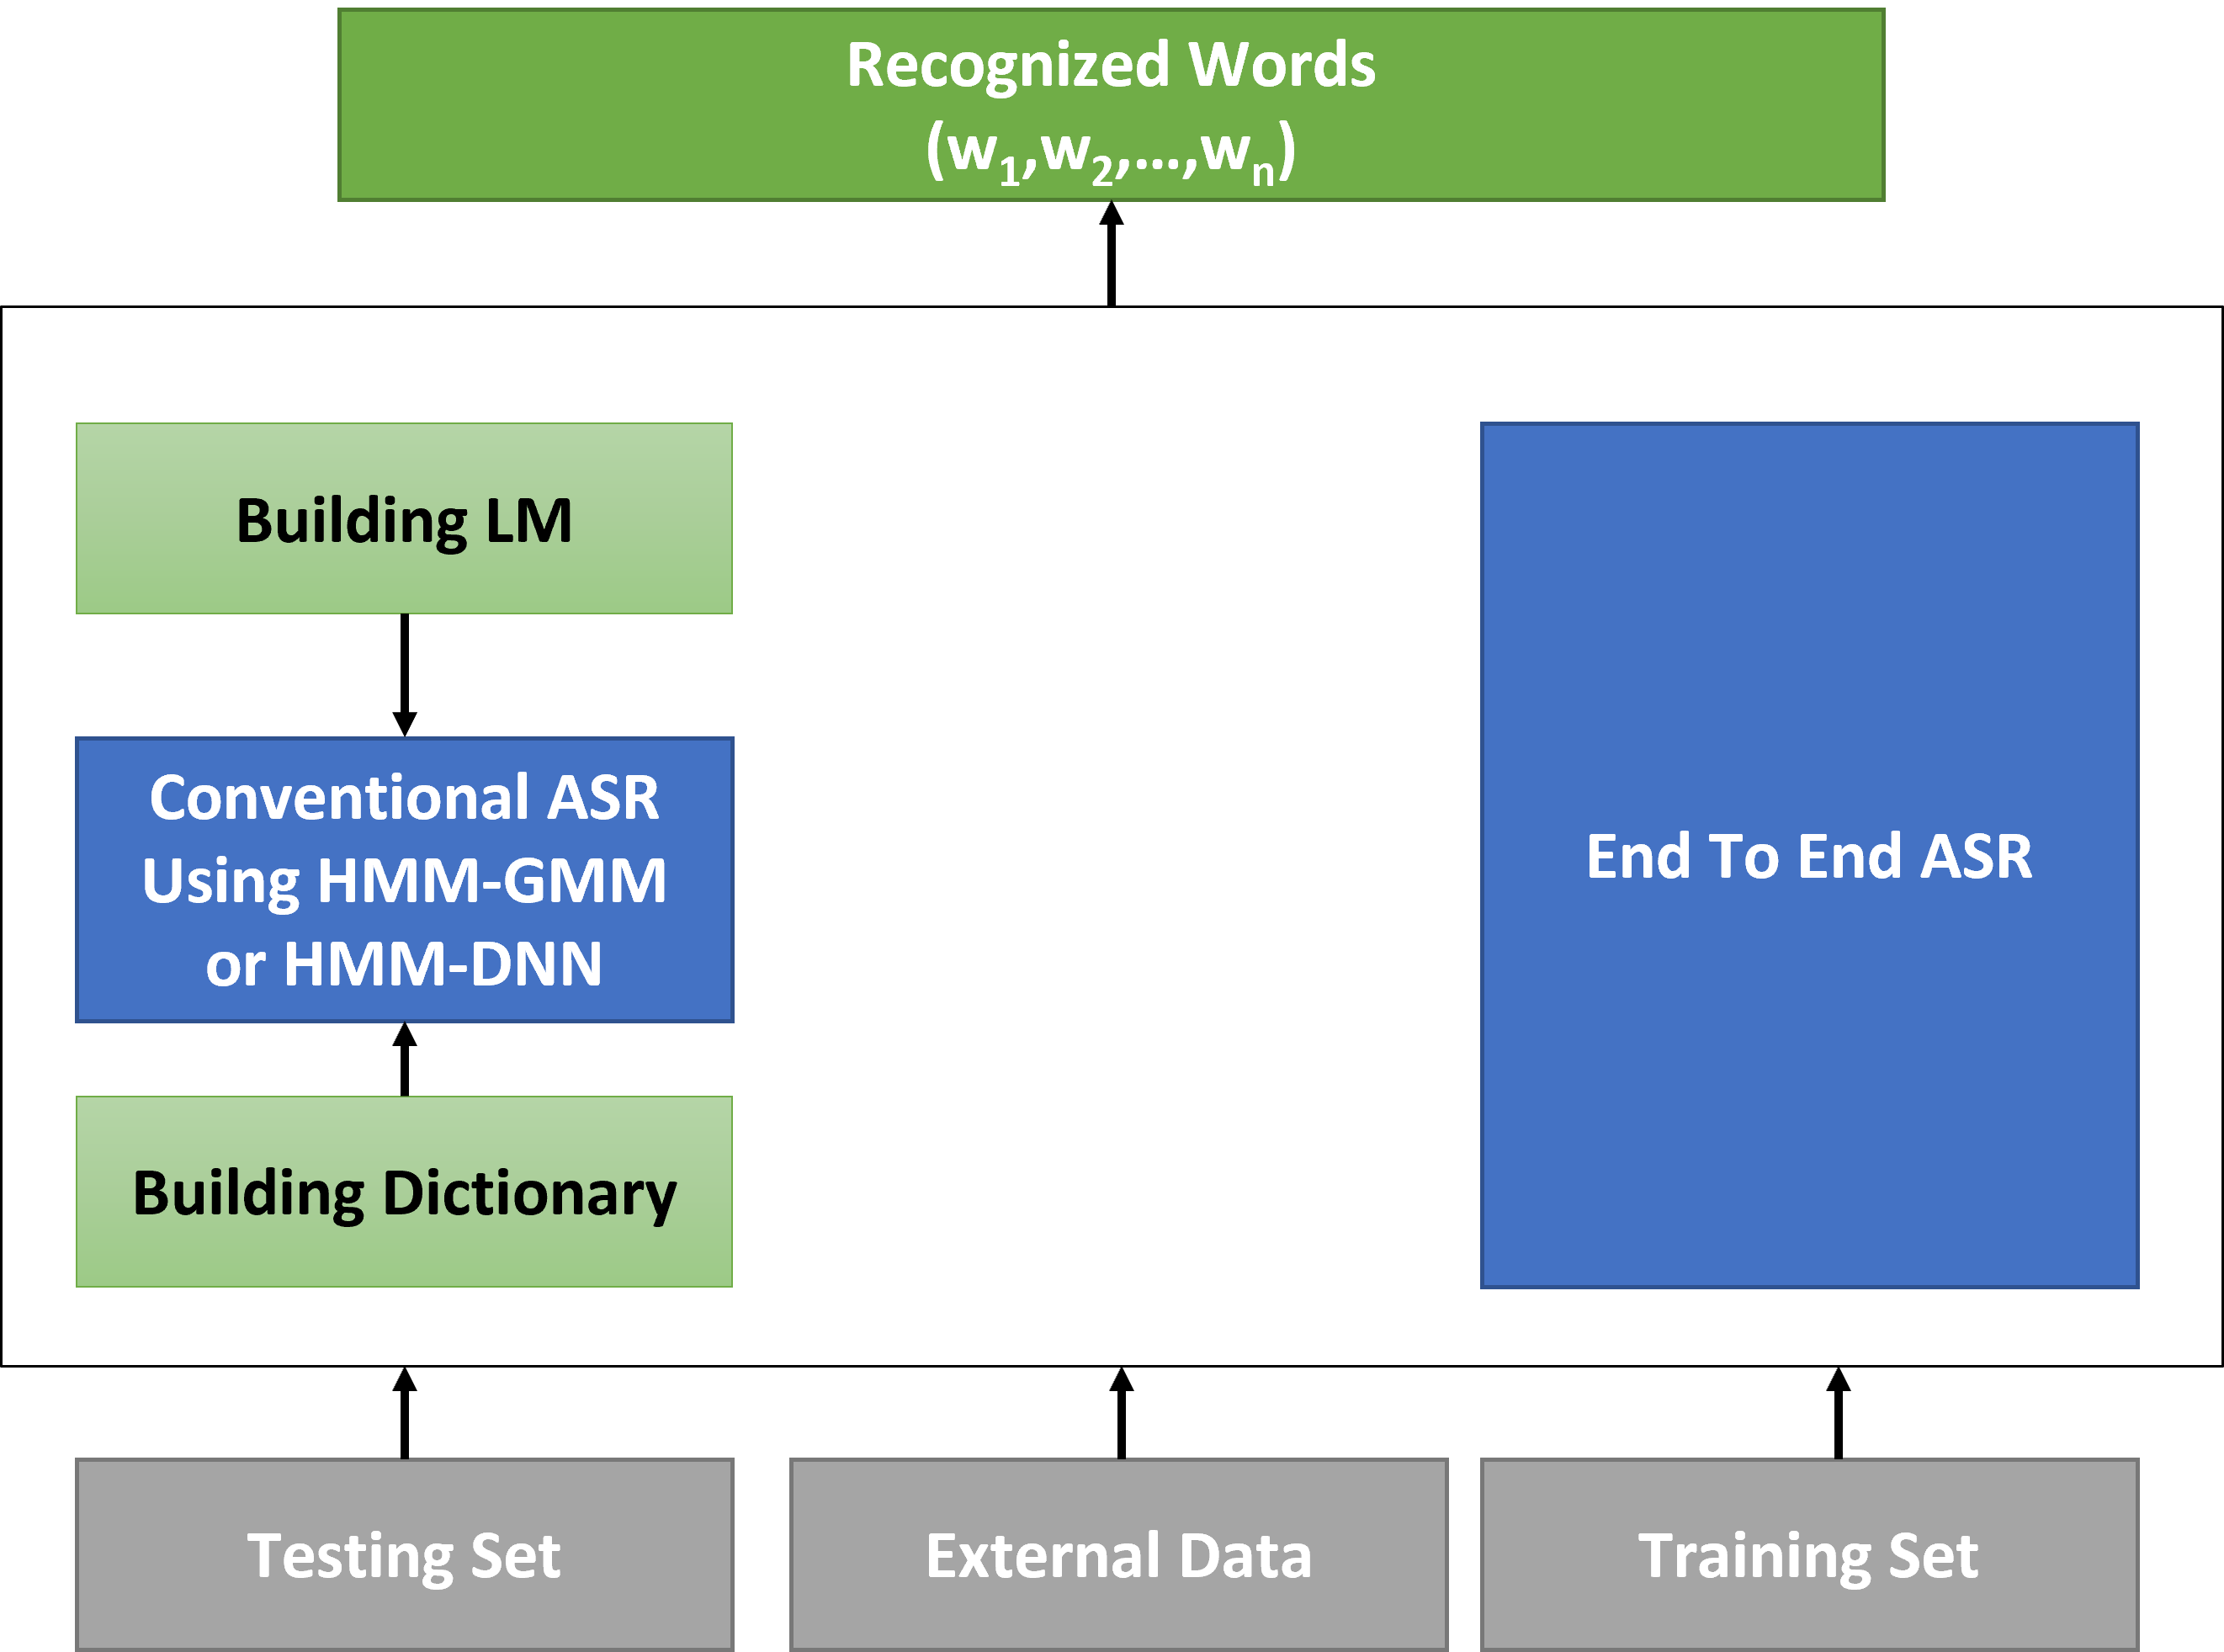
\includegraphics[width=0.6\textwidth]{img/E2EvsConventional.png}
    \caption{E2E ASR Architecture vs Conventional}
    \label{fig:e2e-asr}
\end{figure}

The E2E model \cite{eeckt_continual_2021} is a system that directly maps input audio sequence to sequence of words or other graphemes \cite{amodei_deep_2015-1, bell_adaptation_2020} using Deep Neural Networks like RNN \cite{sak_long_2014}, CNN \cite{abdel-hamid_exploring_2013}, TDNN \cite{kreyssig_improved_2018} and CNN-TDNN \cite{ghahremani_acoustic_2016}.

\begin{figure}[h]
    \centering
    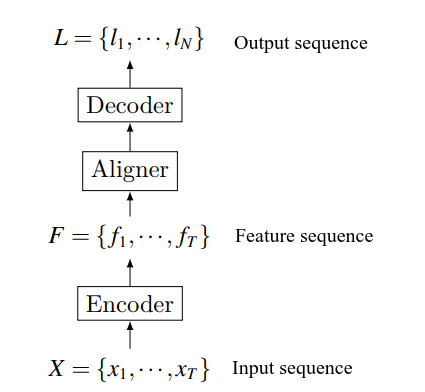
\includegraphics[width=0.4\textwidth]{img/E2E.png}
    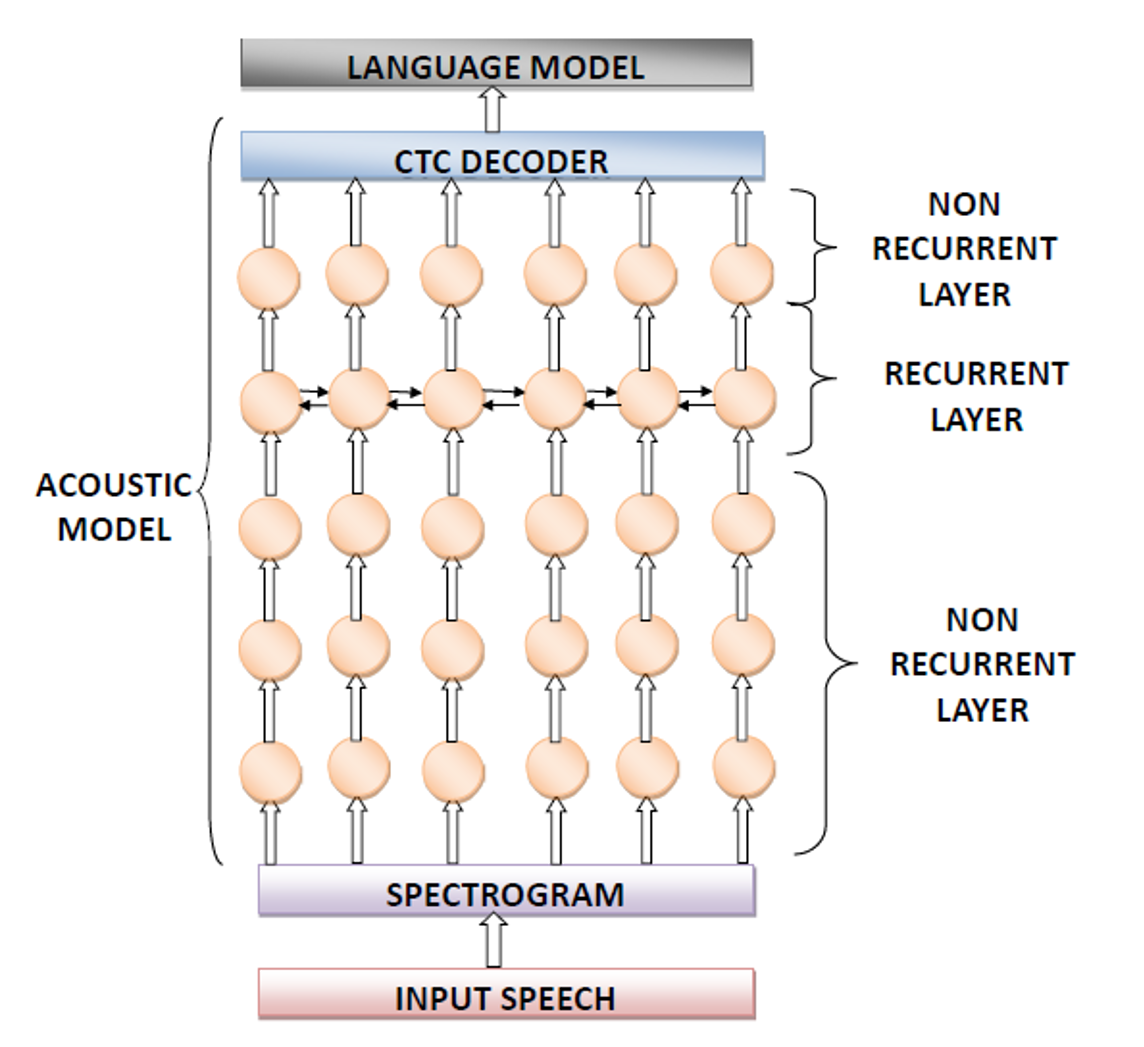
\includegraphics[width=0.4\textwidth]{img/e2est.png}
    \caption{End to End Model}
    \label{fig:e2e-model}
\end{figure}

Despite its triumphs, the use of DNNs in speech processing has the following drawbacks \cite{backstrom_introduction_2022}:

\begin{itemize}
    \item DNN training on a specific dataset does necessarily improve the understanding of the problem. It's a black box because the model's reliability is not known. Although the design process gives some insights about languages, a trained speech recognizer on language "A" does not tell much about speech recognition on language "B" \cite{backstrom_introduction_2022}.
    \item DNN training is highly dependent on the data used to train it e.g. Models can be vulnerable to hidden biases, resulting in poor performance for OOVs or in a different scenario \cite{zhang_strategies_2019}.
    \item A trained DNN solves a specific problem, but does not tell how good the solution is. If a data set represents a circle in the 2D plane, that dataset can be accurately modelled with Sigmoids as non-linearities with a neural network. The neural network only needs to be large enough to handle the task at hand. The network, on the other hand, is several orders of magnitude more complex than the circle equation, which means that even though the network was successfully trained and the model is reasonably accurate, it gives no indication of whether the network's complexity is comparable to the problem's complexity \cite{backstrom_introduction_2022}.
    \item E2E models that are primarily DNN based typically require a large amount of training dataset, 1000 to 100,000 hours of speech to achieve peak performance. Such information is rarely available while also necessitating the purchase of costly hardware and computational resources \cite{kincaid_state_2018}.
    
\end{itemize}

To tackle these issues, the recent model design trend has been to return to classical design paradigms, in which models are based on a in-depth understanding of the problem, particularly in the case of Low-Resource Languages and the parameters of those models are then trained using ML methods \cite{backstrom_introduction_2022}.   

\section{Training ASRs using Statistical Methods with Neural Networks}

Different modules in the HMM-based model employ various technologies and serve different roles. HMM is primarily used at the frame level to perform dynamic time warping, while GMM and DNN are used to compute the emission probability of HMM hidden states \cite{georgescu_kaldi-based_2019}. The HMM-GMM model served as the foundation for many speech recognition systems, but with advancement in deep learning technology DNN was used to calculate the posterior probability of the HMM state instead of the traditional GMM observation-probability. DNN is now used for language and acoustic modelling instead of HMM-GMM model because HMM-DNN outperforms HMM-GMM in terms or accuracy. \cite{dahl_context-dependent_2012}. %and thus becomes the state-of-the-art ASR model.

\begin{figure}[h]
    \centering
    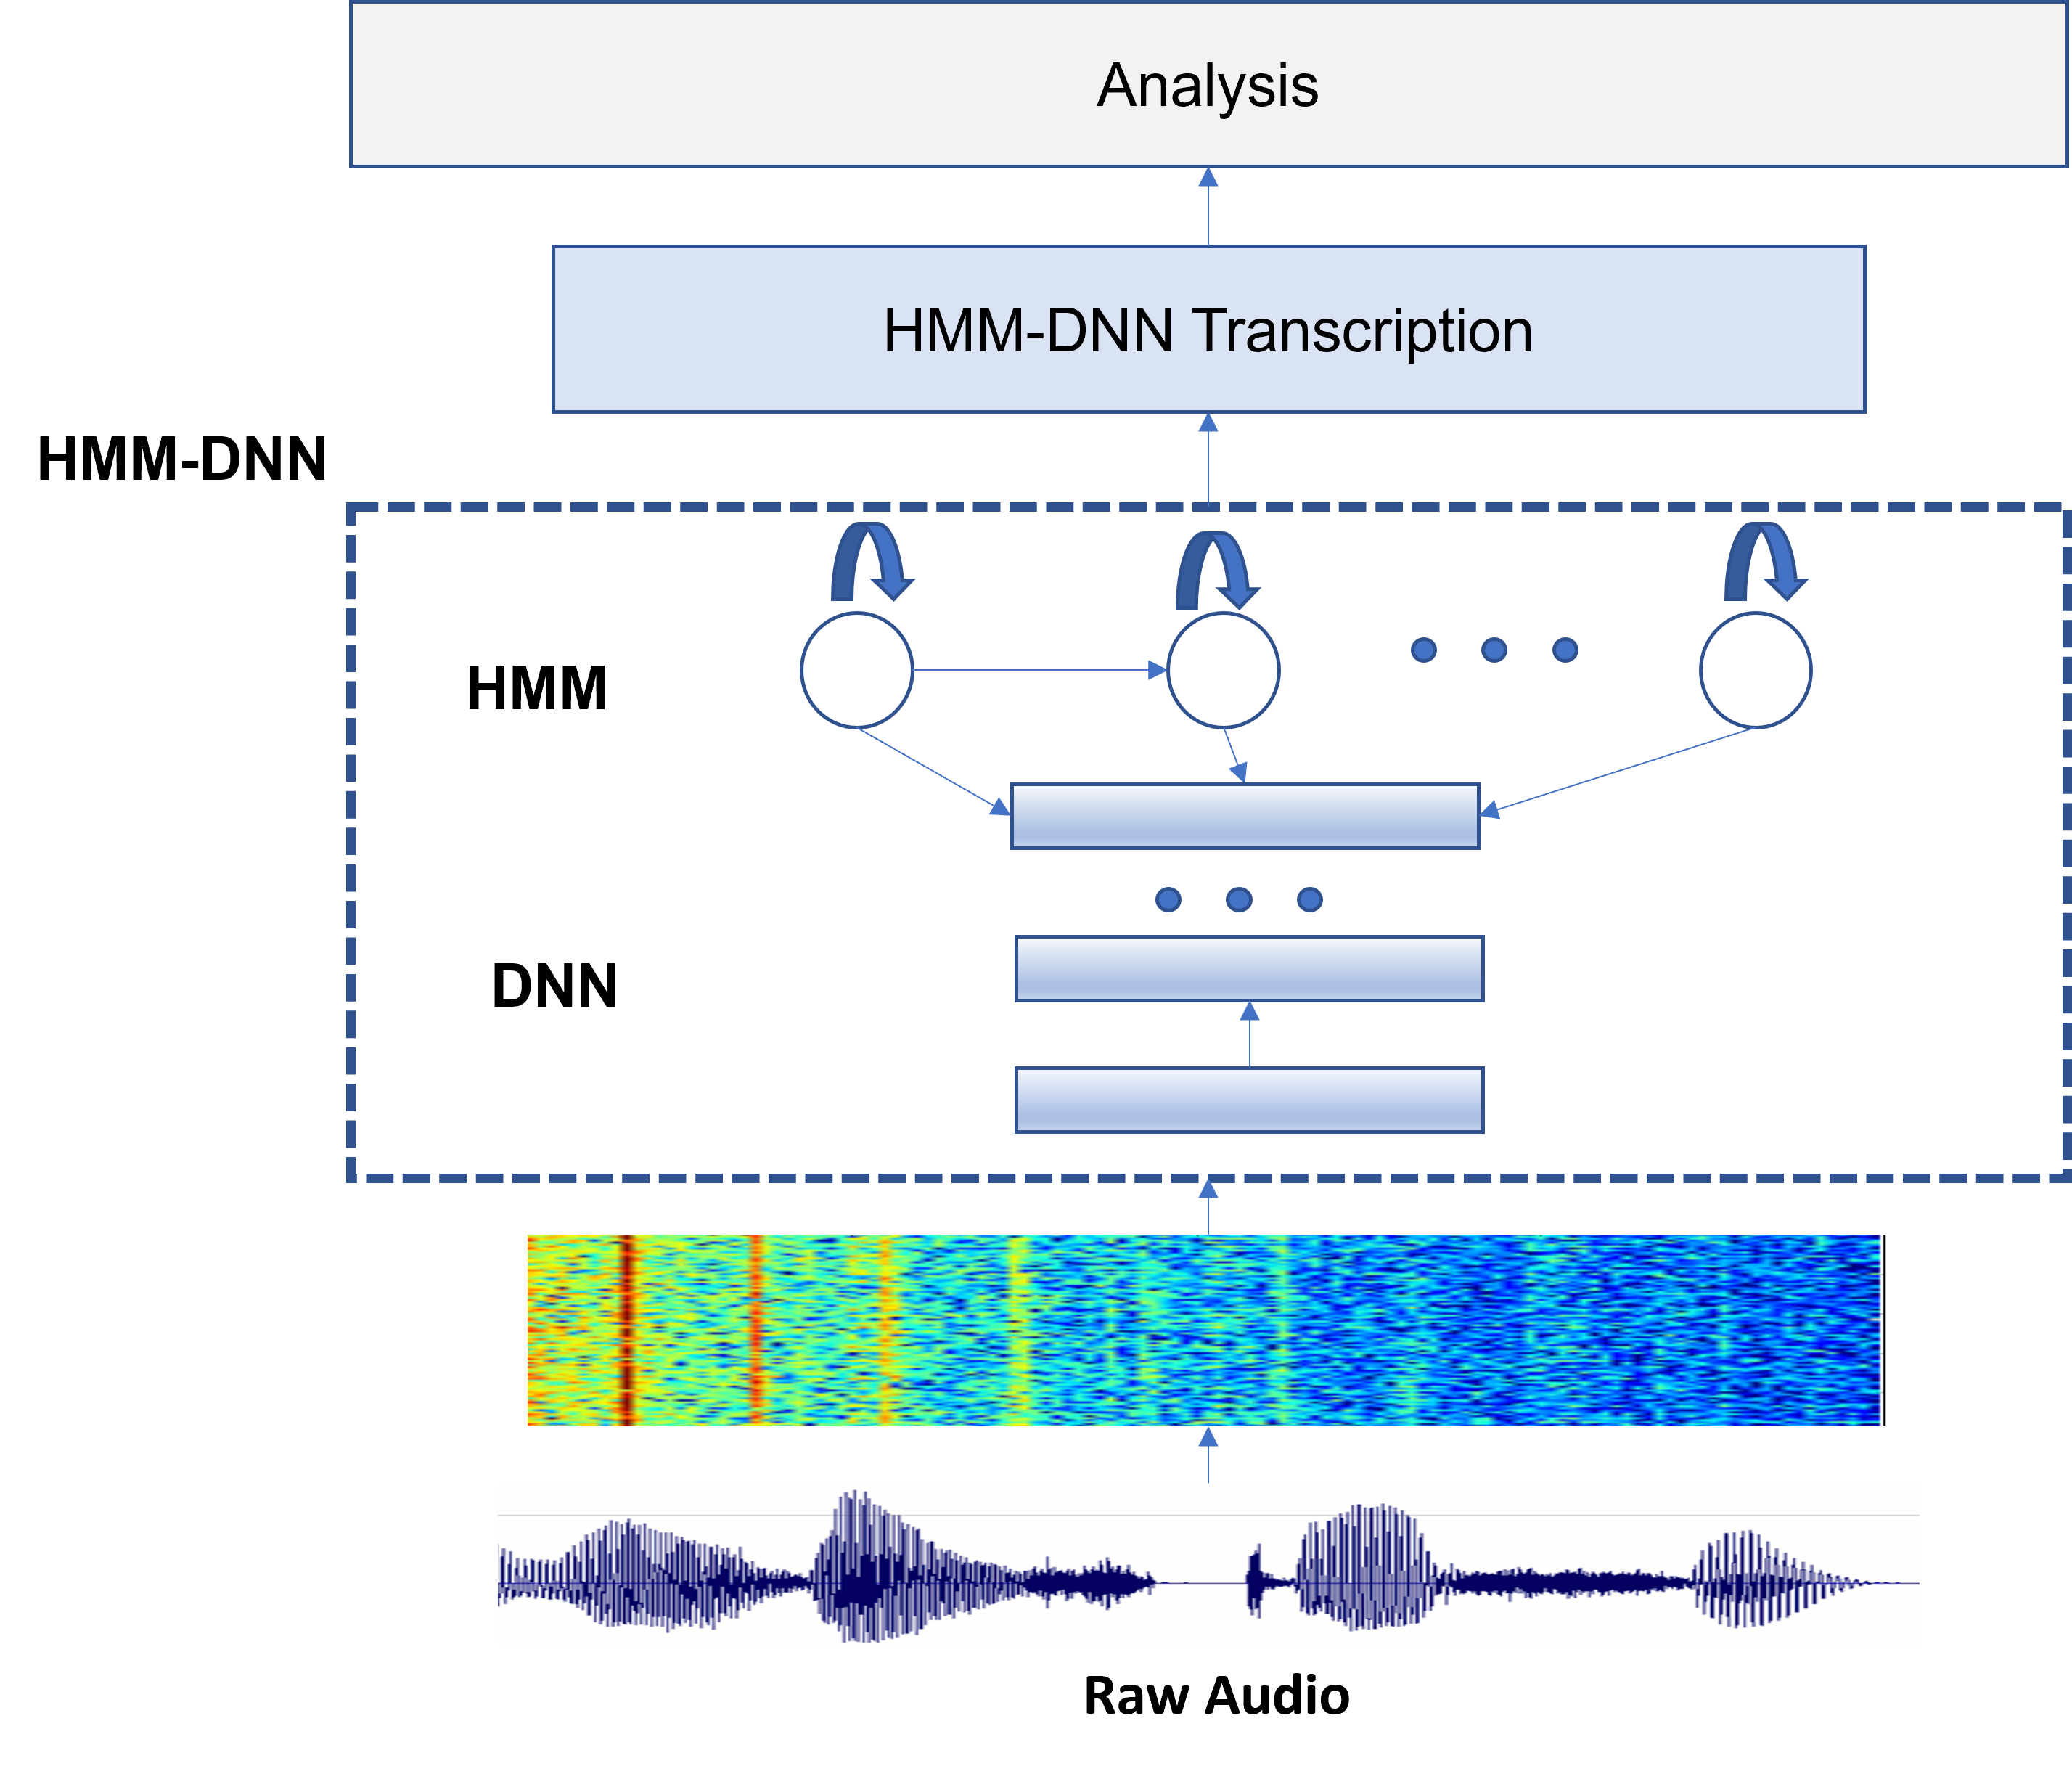
\includegraphics[width=0.5\textwidth]{img/HMM-DNN.png}
    \caption{HMM-DNN Architecture}
    \label{fig:Hmm-dnn-arch}
\end{figure}

One of the first application of HMM–DNN hybrid approach was by Dahl Et al 2012 \cite{dahl_context-dependent_2012} in which Deep neural network model replaced GMM which increased accuracy compared to traditional HMM-GMM legacy system in LVCSR. Many DNN architectures were explored for the acoustic modeling, including Recurrent Neural Networks (RNNs), Bidirectional RNNs (BDRNNs), and deep conditional random fields \cite{graves_speech_2013, hifny_unified_2015}. \cite{vijayaditya_time_2015} proposed a time delay neural network (TDNN) which gave improved results in learning wider temporal dependencies in comparison to models based on DNN or RNN. 

Various studies \cite{smit_advances_2021, li_hybrid_2013, ochiai_speaker_2016} modeled the acoustic component of ASR system using Deep Neural Networks, referred to as Hybrid DNN-HMM approach. Rectified Linear Units (ReLU) and maxout units are commonly used in ASR systems as activation functions to model non-linearity in DNN \cite{backstrom_introduction_2022}. 

\begin{figure}[h]
    \centering
    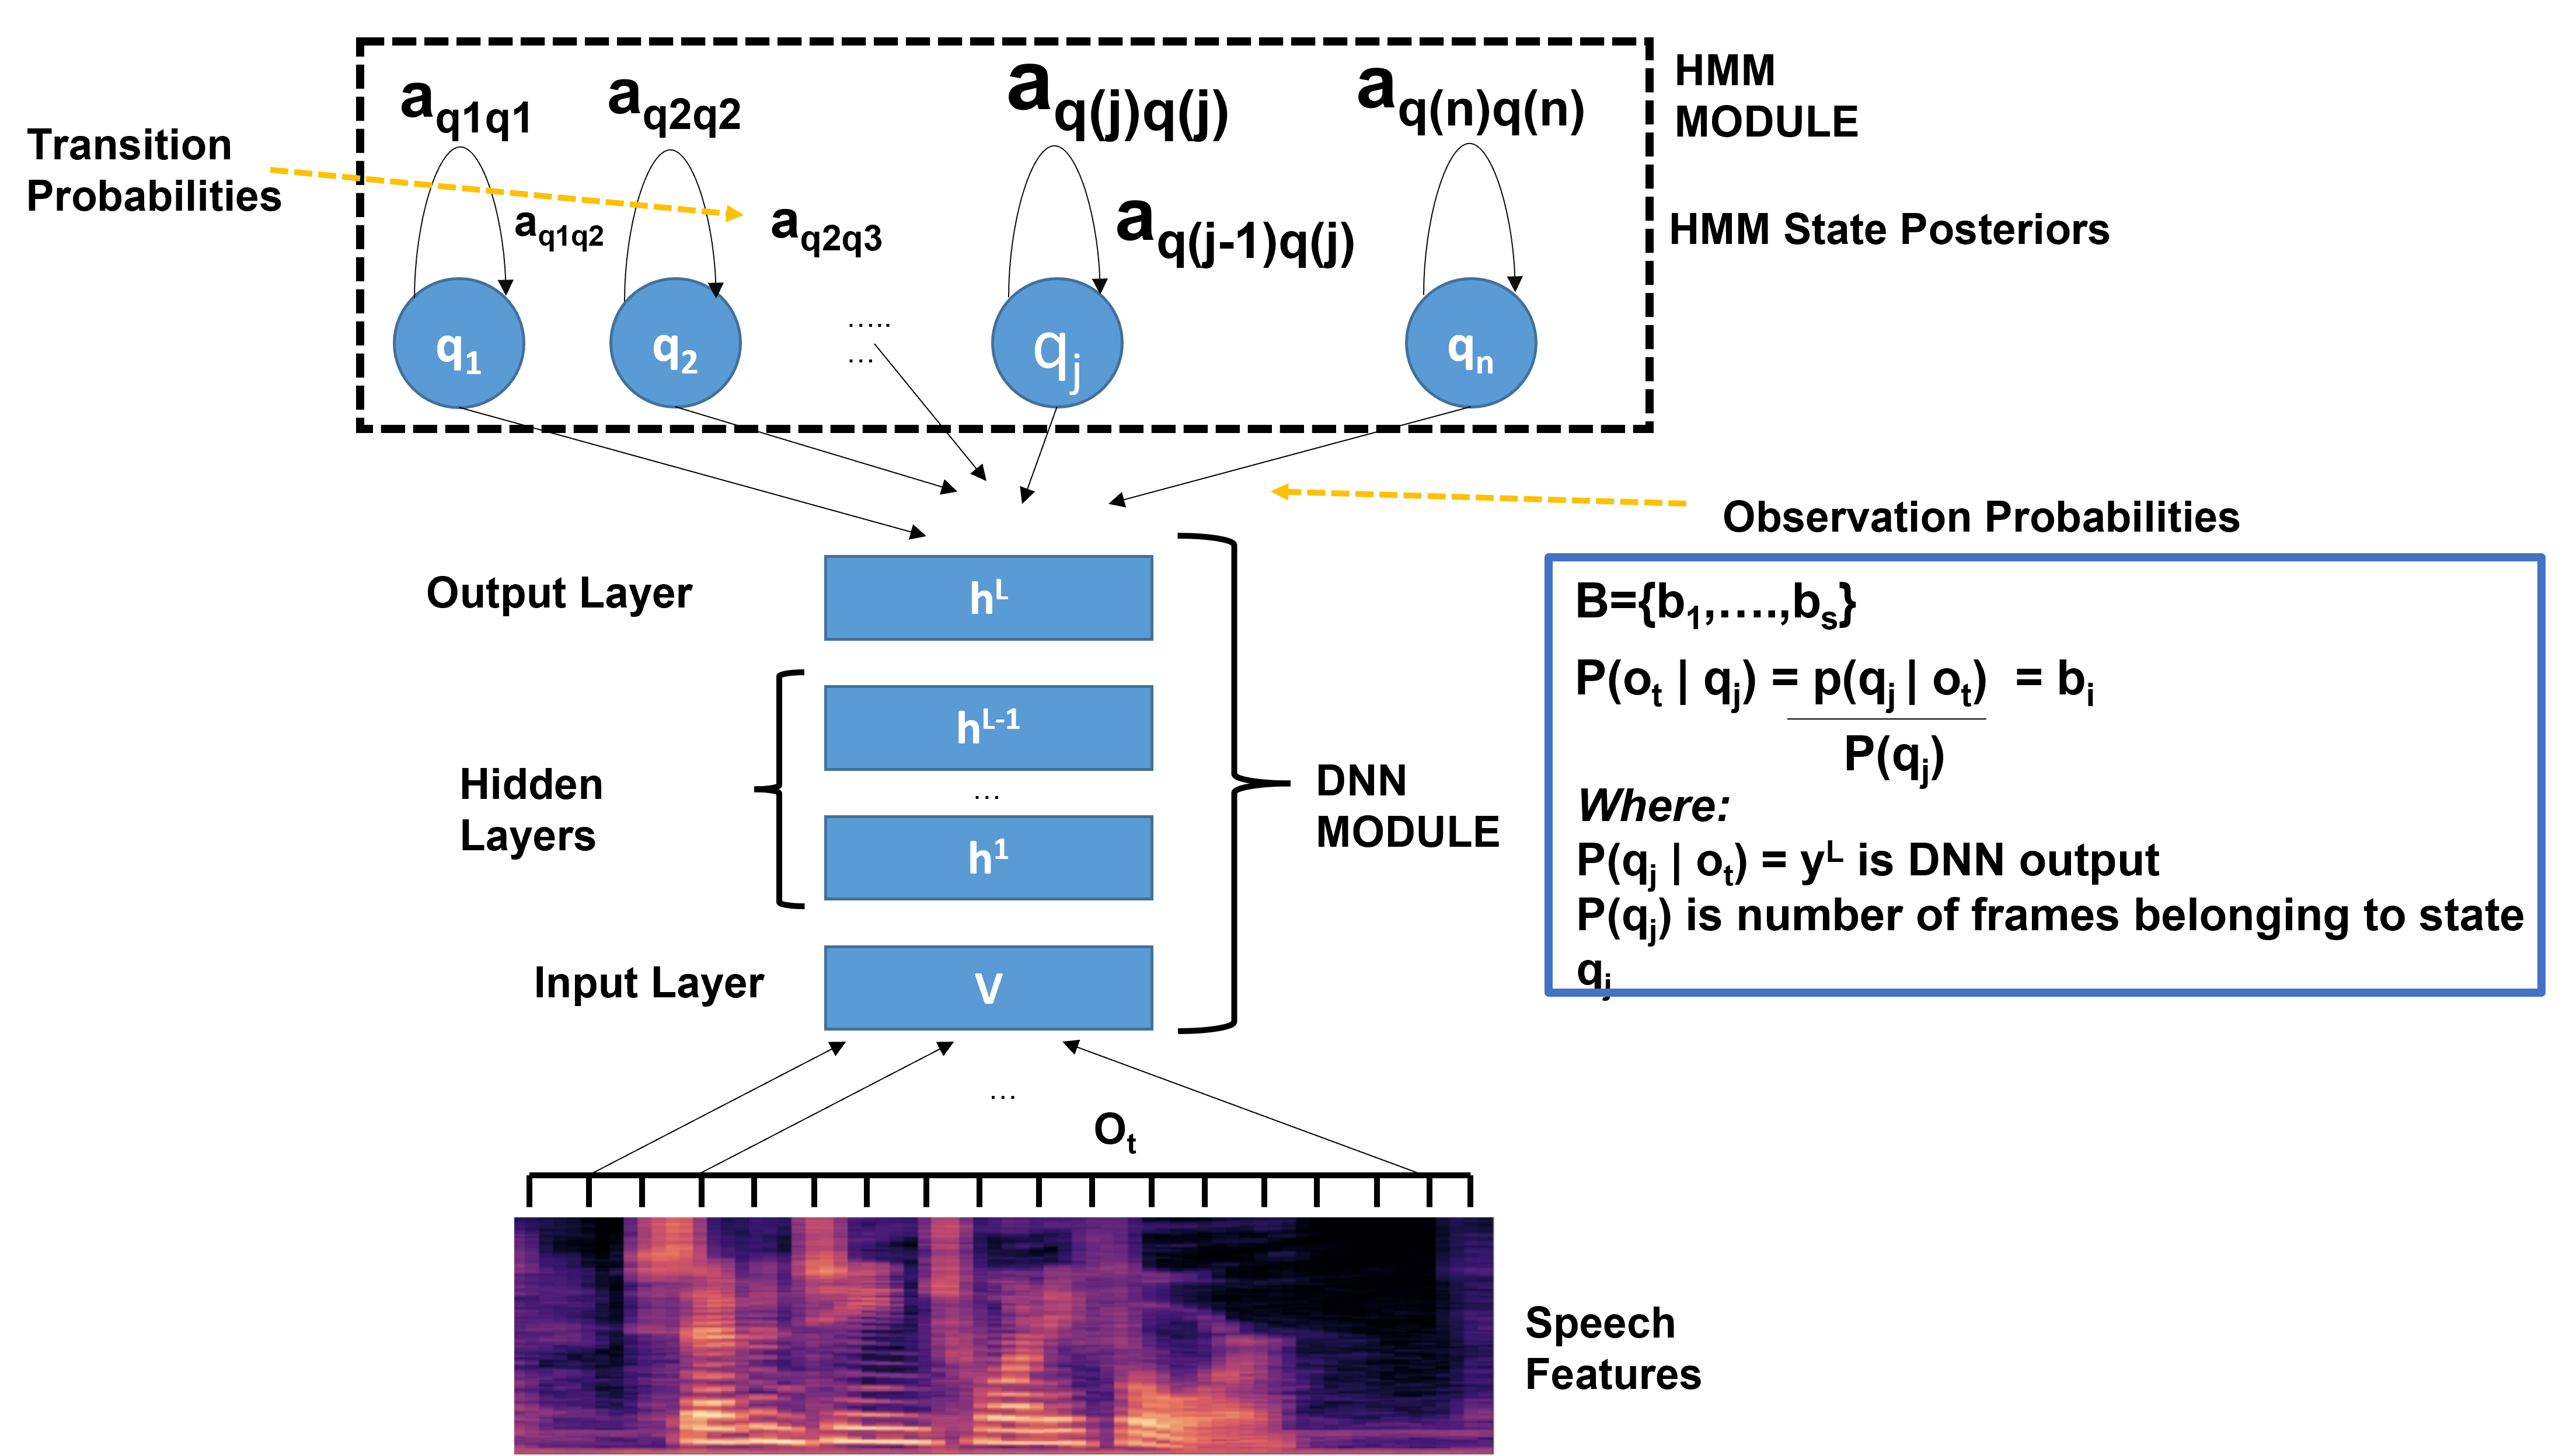
\includegraphics[width=0.95\textwidth]{img/generic-Hmm-DNN.png}
    \caption{Working of HMM-DNN ASR}
    \label{fig:working-hmm-dnn}
\end{figure}

In HMM DNN System audio is broken into segments and frames and features are taken as input in the input layer. This input is passed via Hidden layers into output Layer on which we apply HMM state posteriors attained from observation and Transition Probabilities. DNN models the scaled observation likelihood of all senones or tied Triphone states, while HMM models the sequential property of speech signals. The same DNN is replicated at various points in time \cite{hussein_arabic_2022}.

Hidden units complicate training weights because each hidden unit indirectly affects the error function via all output units. Credit assignment problem 
involves determining hidden unit error and the importance of the input-hidden weight to the output unit which is solved by back-propagating gradients through the network - the gradient for a hidden unit output with respect to error can be calculated as the weighted sum of the deltas of the connected output units (Propagate the values backwards through the network). The back-propagation of error or back-prop algorithm allows the propagation of error gradients through a deep network in order to perform gradient descent training \cite{dahl_context-dependent_2012}.

%\begin{figure}[h!]
%    \centering
%    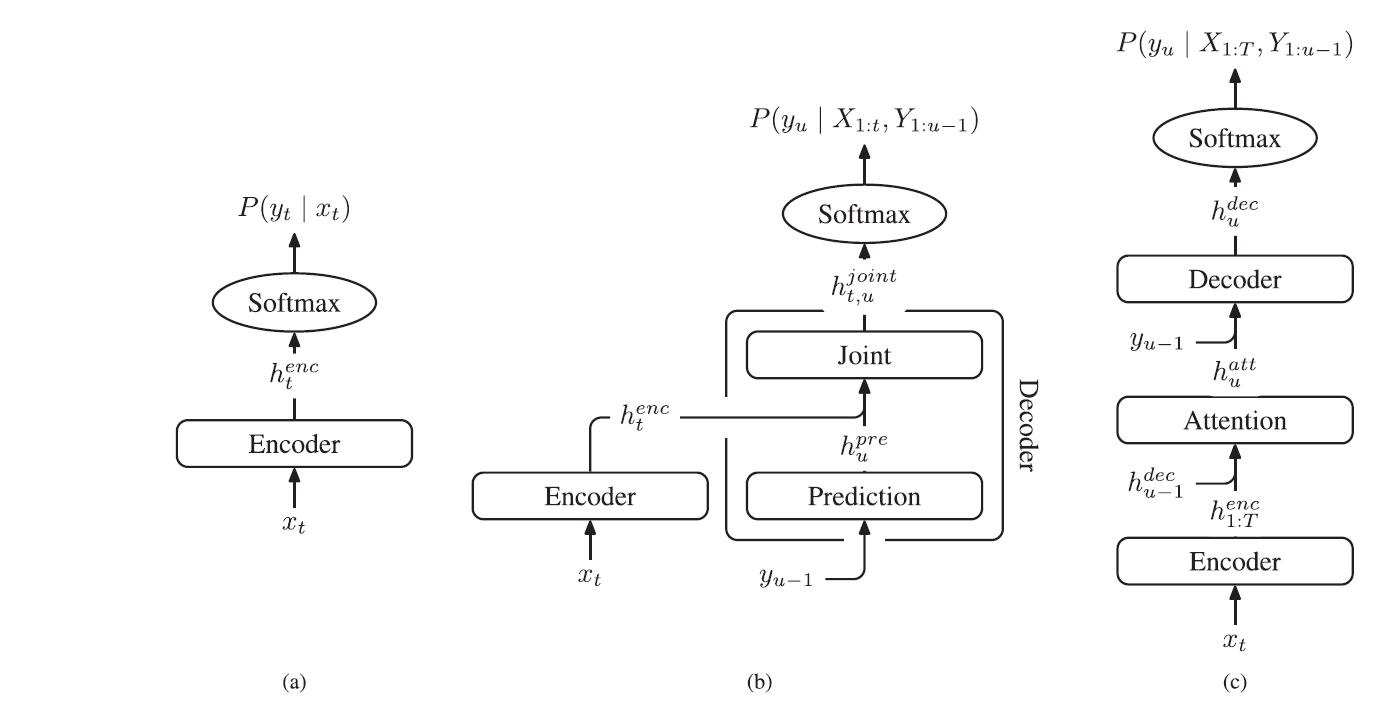
\includegraphics[width=0.9\textwidth]{img/hybridande2e.png}
%    \caption{NN architectures for Hybrid NN/HMM and E2E}
%    \label{fig:hybrid-e2e}
%\end{figure}

%Figure \ref{fig:hybrid-e2e} shows NN architectures used for hybrid NN/HMM and end-to-end (CTC, RNN-T, AED) speech recognition systems:
%\begin{enumerate}[label=(\alph*)]
%    \item Scheme of NN in NN/HMM hybrid systems and CTC
%    \item RNN Transducer (RNN-T) architecture
%    \item Attention based encoder-decoder (AED) end-to-end systems architecture in which $x_{t}$ denotes input acoustic feature vectors; $h_{t}$ and $h_{u}$ denotes hidden layers, and $y_{t}$, $y_{u}$ denotes output labels, depends if they are indexed by time \textit{t} in hybrid and CTC systems or only by output label \textit{u} in parts of RNN-T and AED systems. The encoders use a wide temporal context as input, in practice, even the whole acoustic sequence in the case of most CTC and AED models.
%\end{enumerate}

%\subsection{Context Dependent Hybrid HMM-DNN}
Context-dependent HMM/GMM system is trained on the same data for a Context-Dependent Hybrid HMM-DNN, using a phonetic decision tree to determine the HMM tied states. Then, using the trained HMM/GMM and the training data, Viterbi alignment is performed after which a neural network is trained to map the input speech features to a label representing a context-dependent tied HMM states \cite{dahl_context-dependent_2012}. 

\begin{figure}[h]
    \centering
    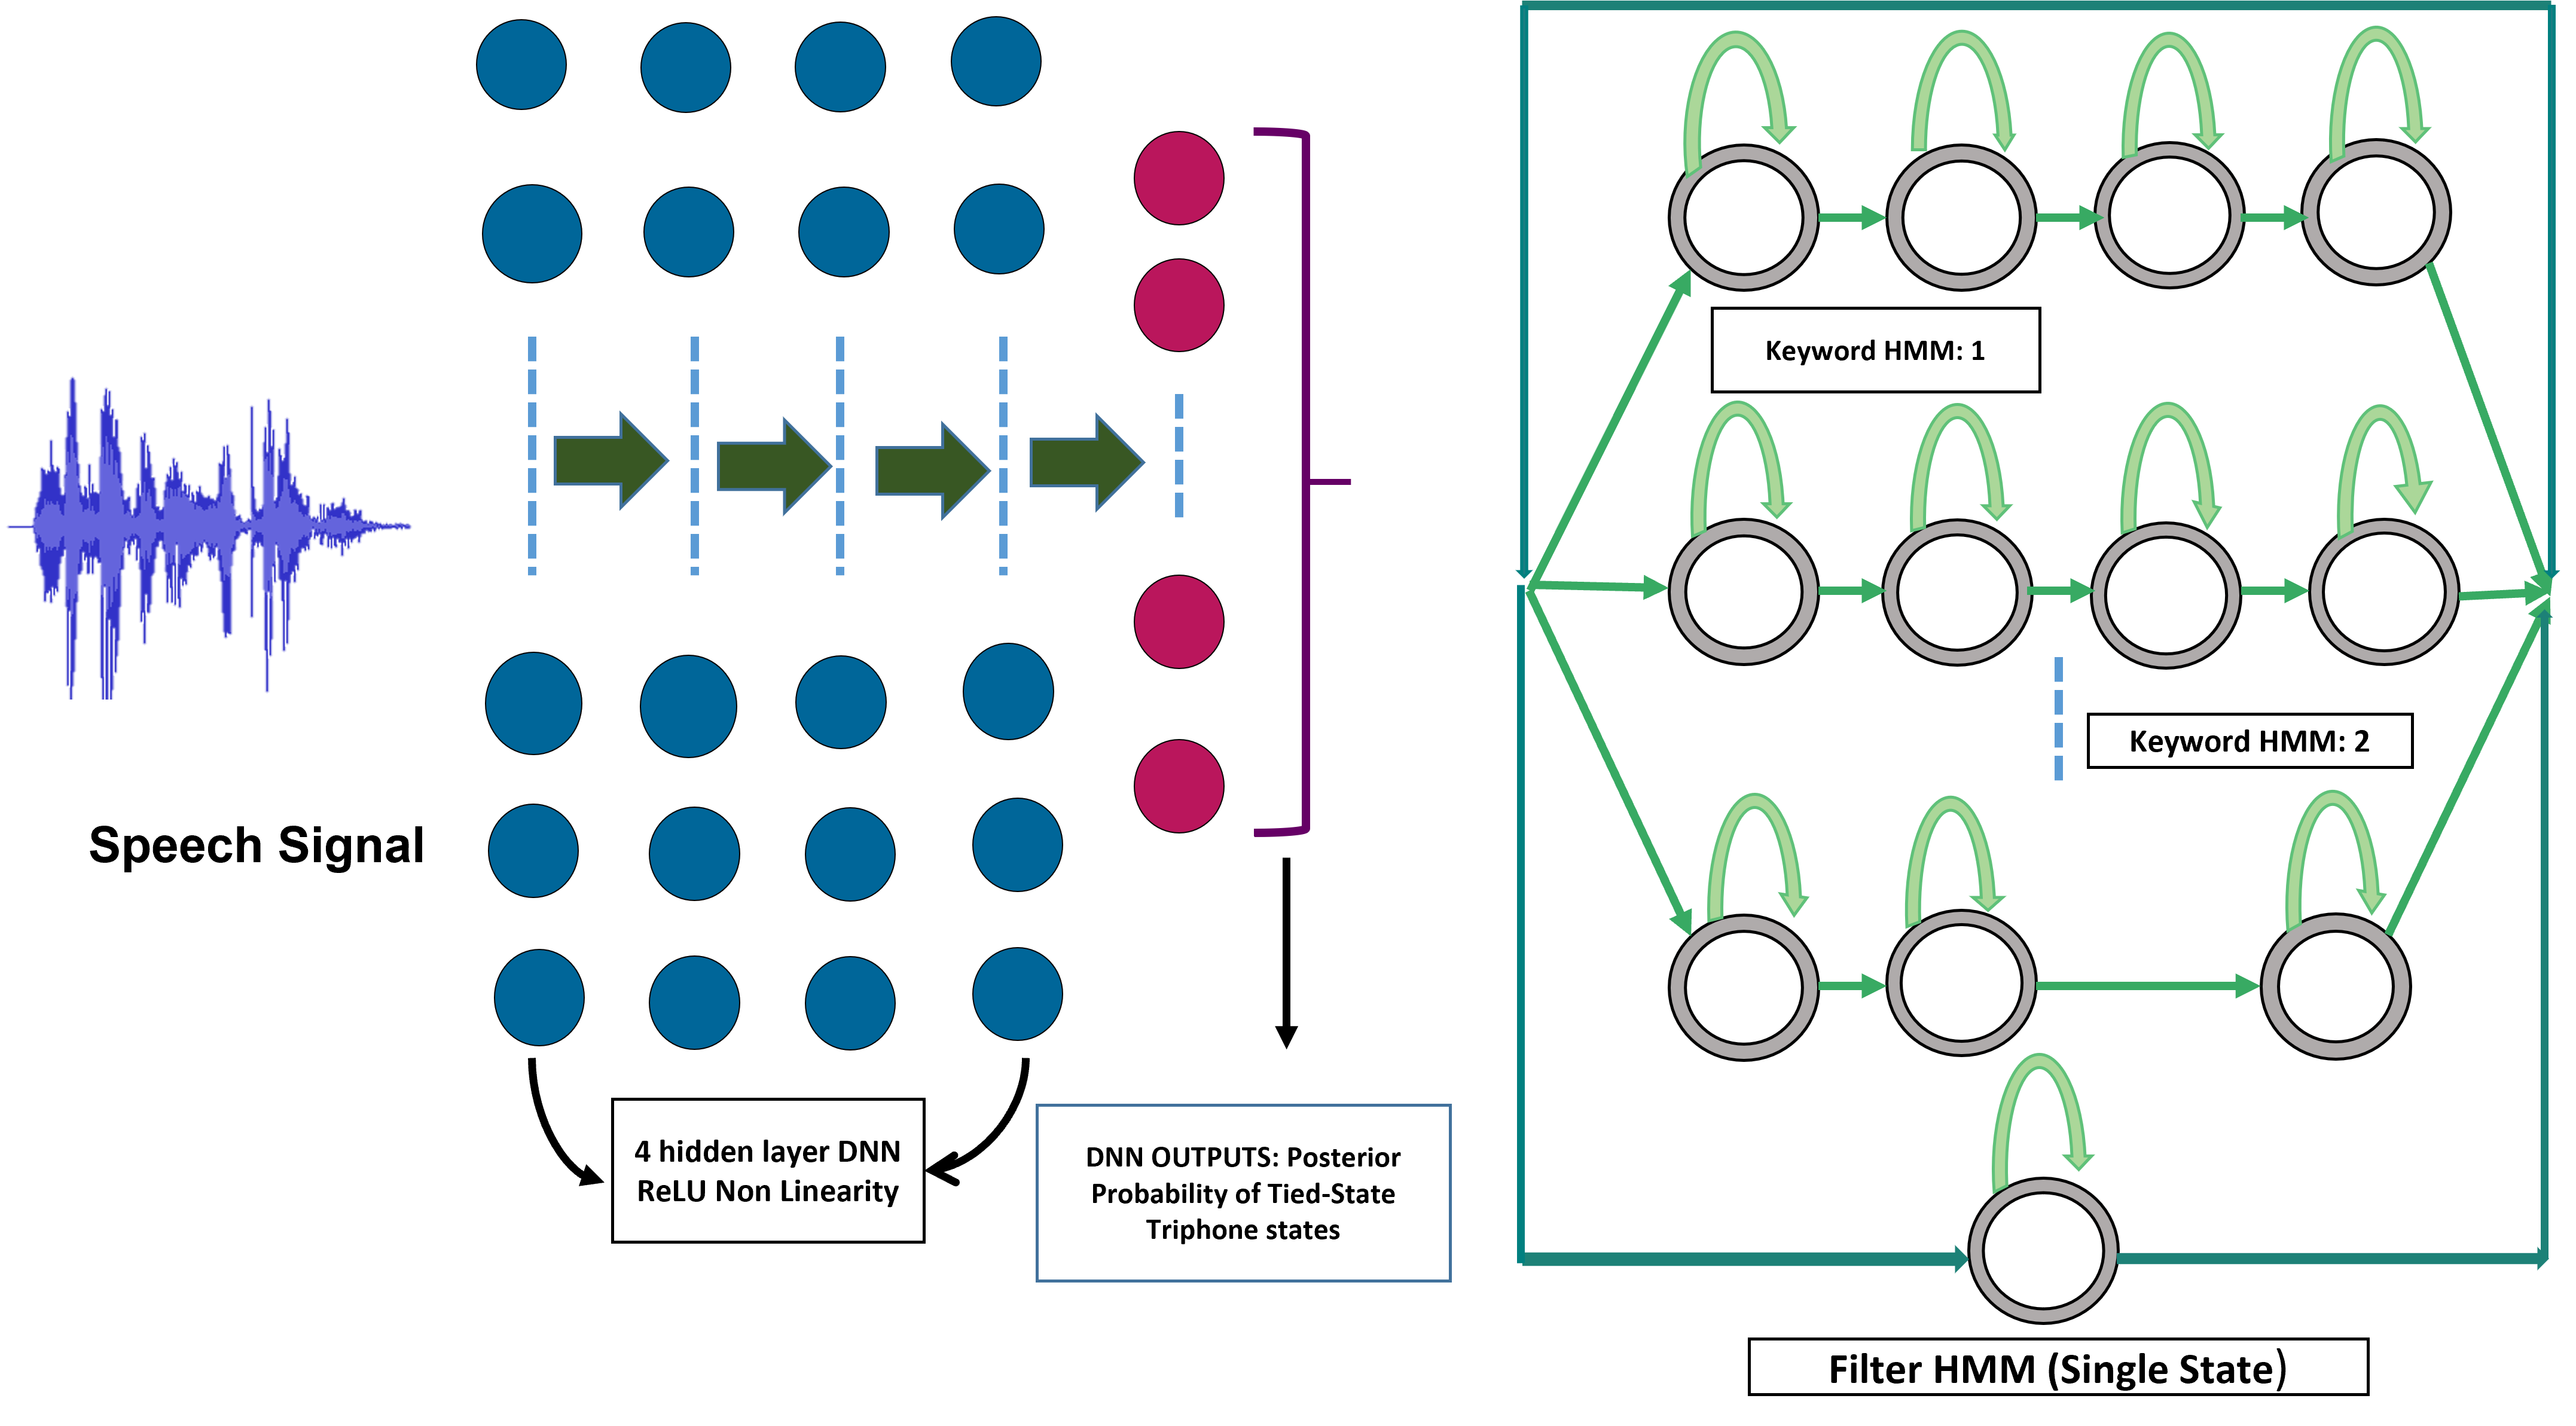
\includegraphics[width=0.95\textwidth]{img/CDHMMDNN.png}
    \caption{Context Dependent HMM-DNN}
    \label{fig:CDHMMDNN}
\end{figure}

The label set is thousands (number of context-dependent tied states) rather than tens of thousands (number of context-independent phones). The Viterbi aligned tied state is then assigned to each frame. Using gradient descent as usual we  train the neural network and decode using the neural network's context-dependent scaled likelihoods \cite{seide_feature_2011}.

\subsection{Benefits of combining HMM and Neural Networks}

Advantages of using HMM-DNN models include:
\begin{itemize}
     \item It is a practical and effective method for ASR deployment on Low Computational Resources compared to Deep Learning Methods. 
     \item It takes less time to train in contrast to Deep Learning Methods \cite{naeem_subspace_2020}.
    \item Maintains the Structure that is required for a Language and Speech Processing System based on which the computer can understand the language better \cite{kincaid_state_2018}. Hence this works better in an environment where the context of speech is of the essence and has been applied for Continuous Speech Recognition as well \cite{backstrom_introduction_2022, morgan_continuous_1995}. 
    \item DNN-HMM can extend the labelling ability of GMM-HMM when the hidden layer and hidden unit numbers are set up properly in comparison to GMM-HMMs, shallow-NN-HMMs, and Multi-layer Perceptrons HMMs (MLPHMMs). Thus, DNN-HMMs with discriminative pre-training can produce good results in our scenario as well \cite{li_hybrid_2013}.
    \item HMM–DNN (especially TDNN) is streamable while E2E-transformer is not \cite{ritter_neural_2019}. 
    \item Computationally intensive compared to E2E Systems \cite{kincaid_brief_2018}.
    \item E2E modelling is less mature than hybrid modelling, and much of the research on E2E modelling is focused on improving general modelling technology \cite{backstrom_introduction_2022}. 
    \item Easily models correlated features like spectral features and input context includes multiple data-frames at input \cite{backstrom_introduction_2022}. 
    \item Because E2E models typically contain sub-networks corresponding to the acoustic model and language model in hybrid models, most adaptation technologies successfully applied to hybrid models by adapting acoustic model or language model can also work well for E2E models \cite{backstrom_introduction_2022}. %Most adaptation technologies successfully applied to hybrid models by adapting acoustic model or language model can also work well for E2E models \cite{backstrom_introduction_2022} since E2E models typically contain sub-networks corresponding to the acoustic model and language model in hybrid models.
    \item Greater flexibility than GMMs because it is not made of nearly local components since GMMs are inefficient for non-linear class boundaries \cite{bell_adaptation_2021}.
    \item NNs can simultaneously model multiple events in the input compared to GMMs, i.e. different sets of hidden units modelling each event, whereas GMMs assume generation of each from by a single mixture component \cite{hussein_arabic_2022}.
    \item NNs can learn more complex representations compared to GMMs and higher-level features such as tandem, posteriorgrams, bottleneck features (like in TDNN) etc \cite{liu_time_2019}.
    \item Components in hybrid HMM-DNN models are optimised separately, whereas E2E models use a single objective function which is why E2E models tend to memorise the training data more, making generalisation or robustness to unseen data difficult for E2E models. Thus, adaptation to a new environment or domain is critical to the large-scale application of E2E models \cite{backstrom_introduction_2022}. 
\end{itemize}

However, HMM–DNN models have some drawbacks like model complexity i.e. complicated to implement since it deploys a modular design, separately training different modules for acoustic modeling, pronunciation lexicon, and language modeling,  requiring of linguistic resources \cite{hussein_arabic_2022}. But as a trade-off for performance, data-set and computation requirement, in our scenario, Using HMM-DNN makes the most sense \cite{georgescu_performance_2021}.

\subsection{Using Maximum Mutual Information Model for HMM-DNN Systems}

Discriminative objective functions like Maximum Mutual Information (MMI) or Maximum Conditional Likelihood Estimation objective functions are trained to maximize the gap between the correct and incorrect answers, or to differentiate between right and wrong answers instead of assigning high weights values to the correct sequences which helps training model to improve the correct output sequence prediction, while making incorrect sequences less likely \cite{povey_purely_2016}. 

Deep networks excel in feature extraction and discovering correlation among them which allows exploitation of contents in making predictions. DNN can be used in ASR to classify phones based on the features extracted in acoustic frames. It is treated like a classifier using softmax to output the probability distribution $P(phone | x_{i})$. The softmax pulls up the ground truth while pulls down the others which is the same concept as Maximum Mutual Information Estimation \cite{wiesner_lattice_2020}.

\begin{equation}
 p_{i} = \frac{e^{score_{i}}}{\sum_{c \in y} e^{score_c}}
\end{equation}

Maximum Likelihood Estimation uses sequence training but it is not discriminative. The softmax function is discriminative here. The term Sequence means that the objective considers the entire utterance rather than "frame-level" objectives such as cross-entropy. The term discriminative refers to the use of an objective function that supposedly optimises some task-related criteria, and then directly minimising that objective using gradient-based methods \cite{noauthor_lattice_nodate}.

To turn MLE into a discriminative sequence training, the classifier is trained by minimizing the cross-entropy and the model is utilized to generate alignments and lattices which is called the discriminative training phase. 

The second phase is the sequence training. Since both the deep network and the lattice are network objects, they can be trained together. This model is then used to calculate the MMIE or Minimum Phone Error objective with the forward-backward algorithm followed by back-propagation to learn the model parameter \cite{wiesner_lattice_2020}.

MMI objective for ASR can be expressed as \cite{noauthor_lattice_nodate}:
\begin{equation}
    F_{MMI}(\theta) = \sum_{r=1}^{R} log \frac{P_{\theta}((O_{r}|M_{Wr})P(w_{r})}{\sum_{\hat{w}}P_{\theta}(O_{r}|M_{\hat{w}})P(\hat{w})} 
\end{equation}

Where $M_{w}$ is HMM that corresponds to transcription \textit{w}. To normalise the numerator, the objective function accounts for the log-probability of complete utterance in the numerator dividing it by the log probability of all possible utterances in the denominator. Thus, the distributions with the subscript $\theta$ are trained parameterized distributions \cite{wiesner_lattice_2020}.

%\begin{figure}[h]
%    \centering
%    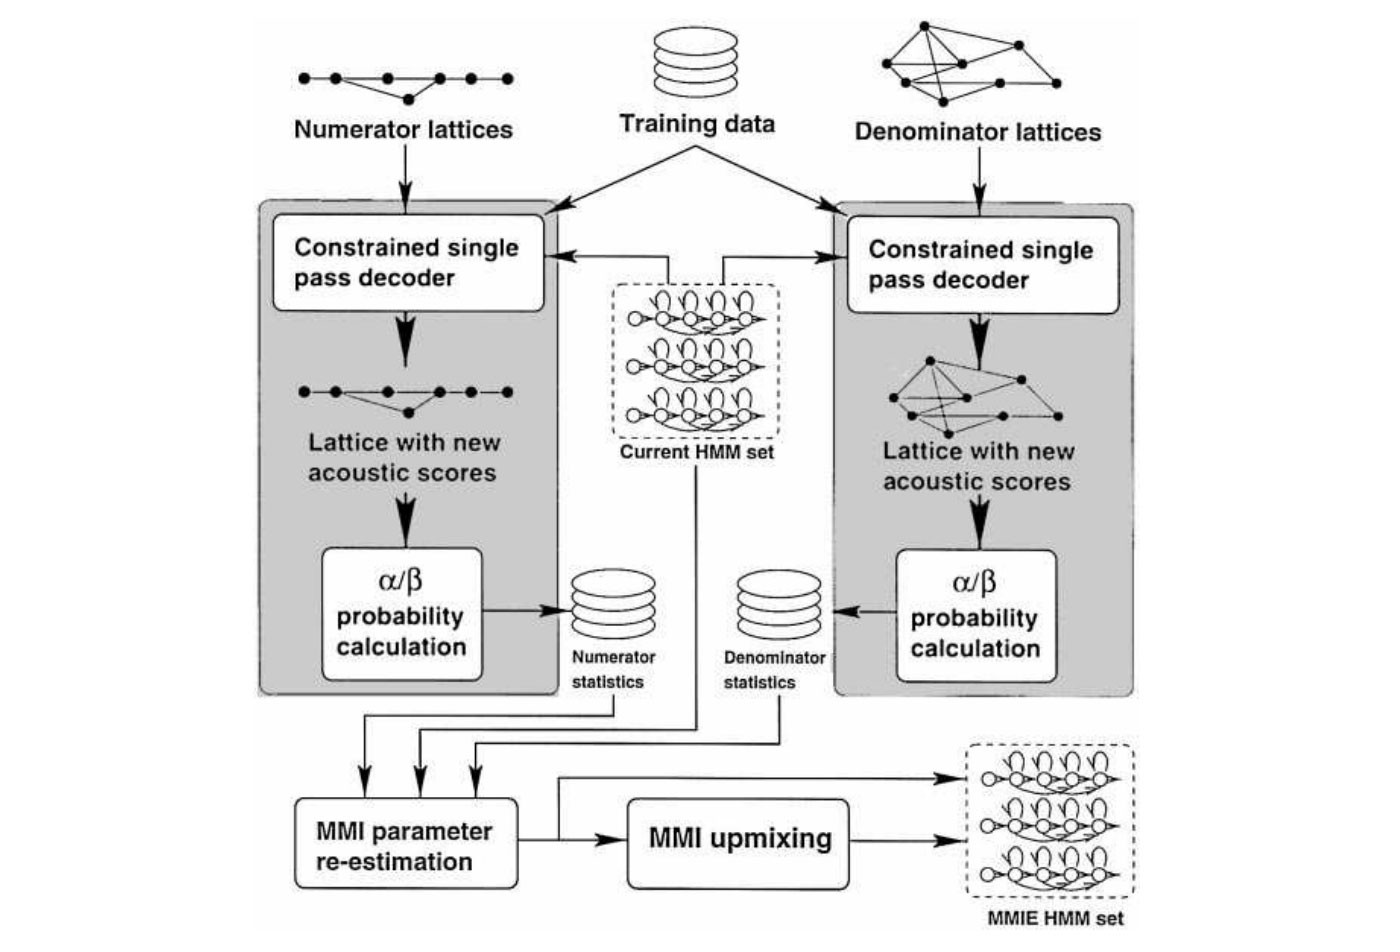
\includegraphics[width=0.9\textwidth]{img/LatticsbasedMMI.jpeg}
%    \caption{Lattice Based MMI system}
%    \label{fig:latt-based-mmi-sys}
%\end{figure}

MMI requires First order Gradient based methods for optimization, such as Stochastic Gradient descent, which requires knowledge of the gradient of the MMI objective with respect to the parameter $\theta$. The neural network function performs forward propagation, while back-propagation computes the corresponding gradient. The state occupancies for the numerator and denominator terms must be computed for the gradient overall objective \cite{daniel_povey_kaldi_nodate}.

Calculating the denominator sum requires summing over an exponentially large amount of word-sequences, which is impractical. Two methods can be used to approximate the sum \cite{noauthor_lattice_nodate}:

\begin{enumerate}
    \item \textbf{N-best list:} This less used and crude method of approximation is computed once and used for all utterances. 
    \item \textbf{Lattice structure:} It can be a word or phone based structure. A path through the lattice denotes a probable phone or word sequence. Lattices require initialization with a trained model which is a drawback, and cross-entropy trained systems are usually used for this purpose. 
\end{enumerate}

%\begin{figure}[h]
%    \centering
%    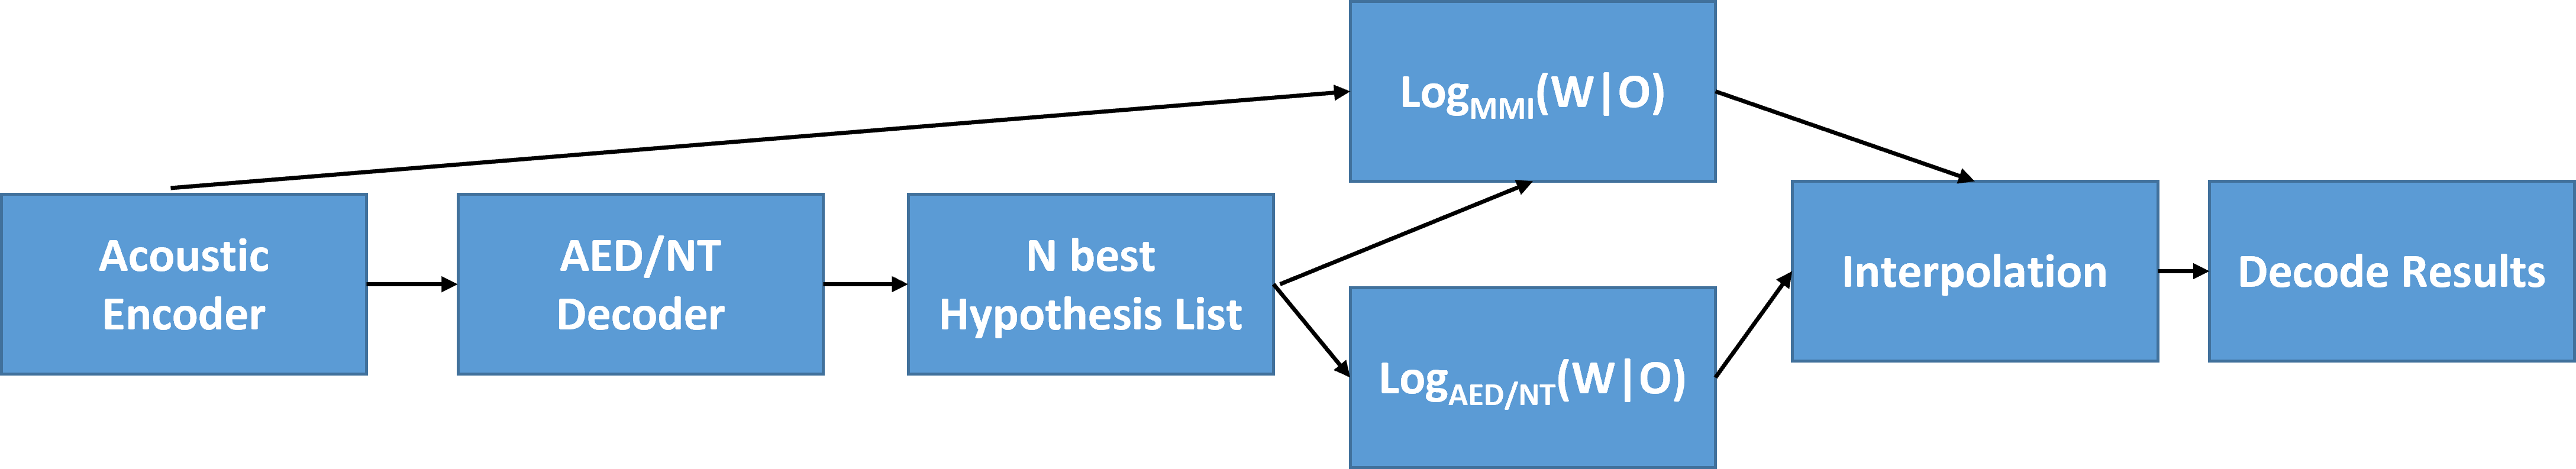
\includegraphics[width=0.9\textwidth]{img/MMISCORING.png}
%    \caption{MMI Scoring}
%    \label{fig:MMI-scoring}
%\end{figure}

The denominator in a lattice-based MMI is first identified by the word lattice. Classifying phones with Deep Learning requires pre-training a deep neural network with cross-entropy. The scaling fudge factor $kappa$ must also be used to correct the overestimation. While training a Deep Neural Network everything seems adhoc but this can be avoided \cite{wiesner_lattice_2020}.

%A composed transducer is generally used in Traditional ASR called H ◦ C ◦ L ◦ G to decode audio. It is a WFST and can be integrated with the deep network classifier. It is a big complex network which can be trained like DNN or DL using back-propagation without the requirement of introduction of a lattice for denominator approximation. Pdf-ids are numerical values of context dependent states given by decoding graphs formed by the decoding algorithms which uses WFSTs to provide graph operations used in acoustic modelling. WFST are used in HMM-GMM models and can also be used along with Deep Neural Network Classifiers.

\begin{figure}[h]
    \centering
    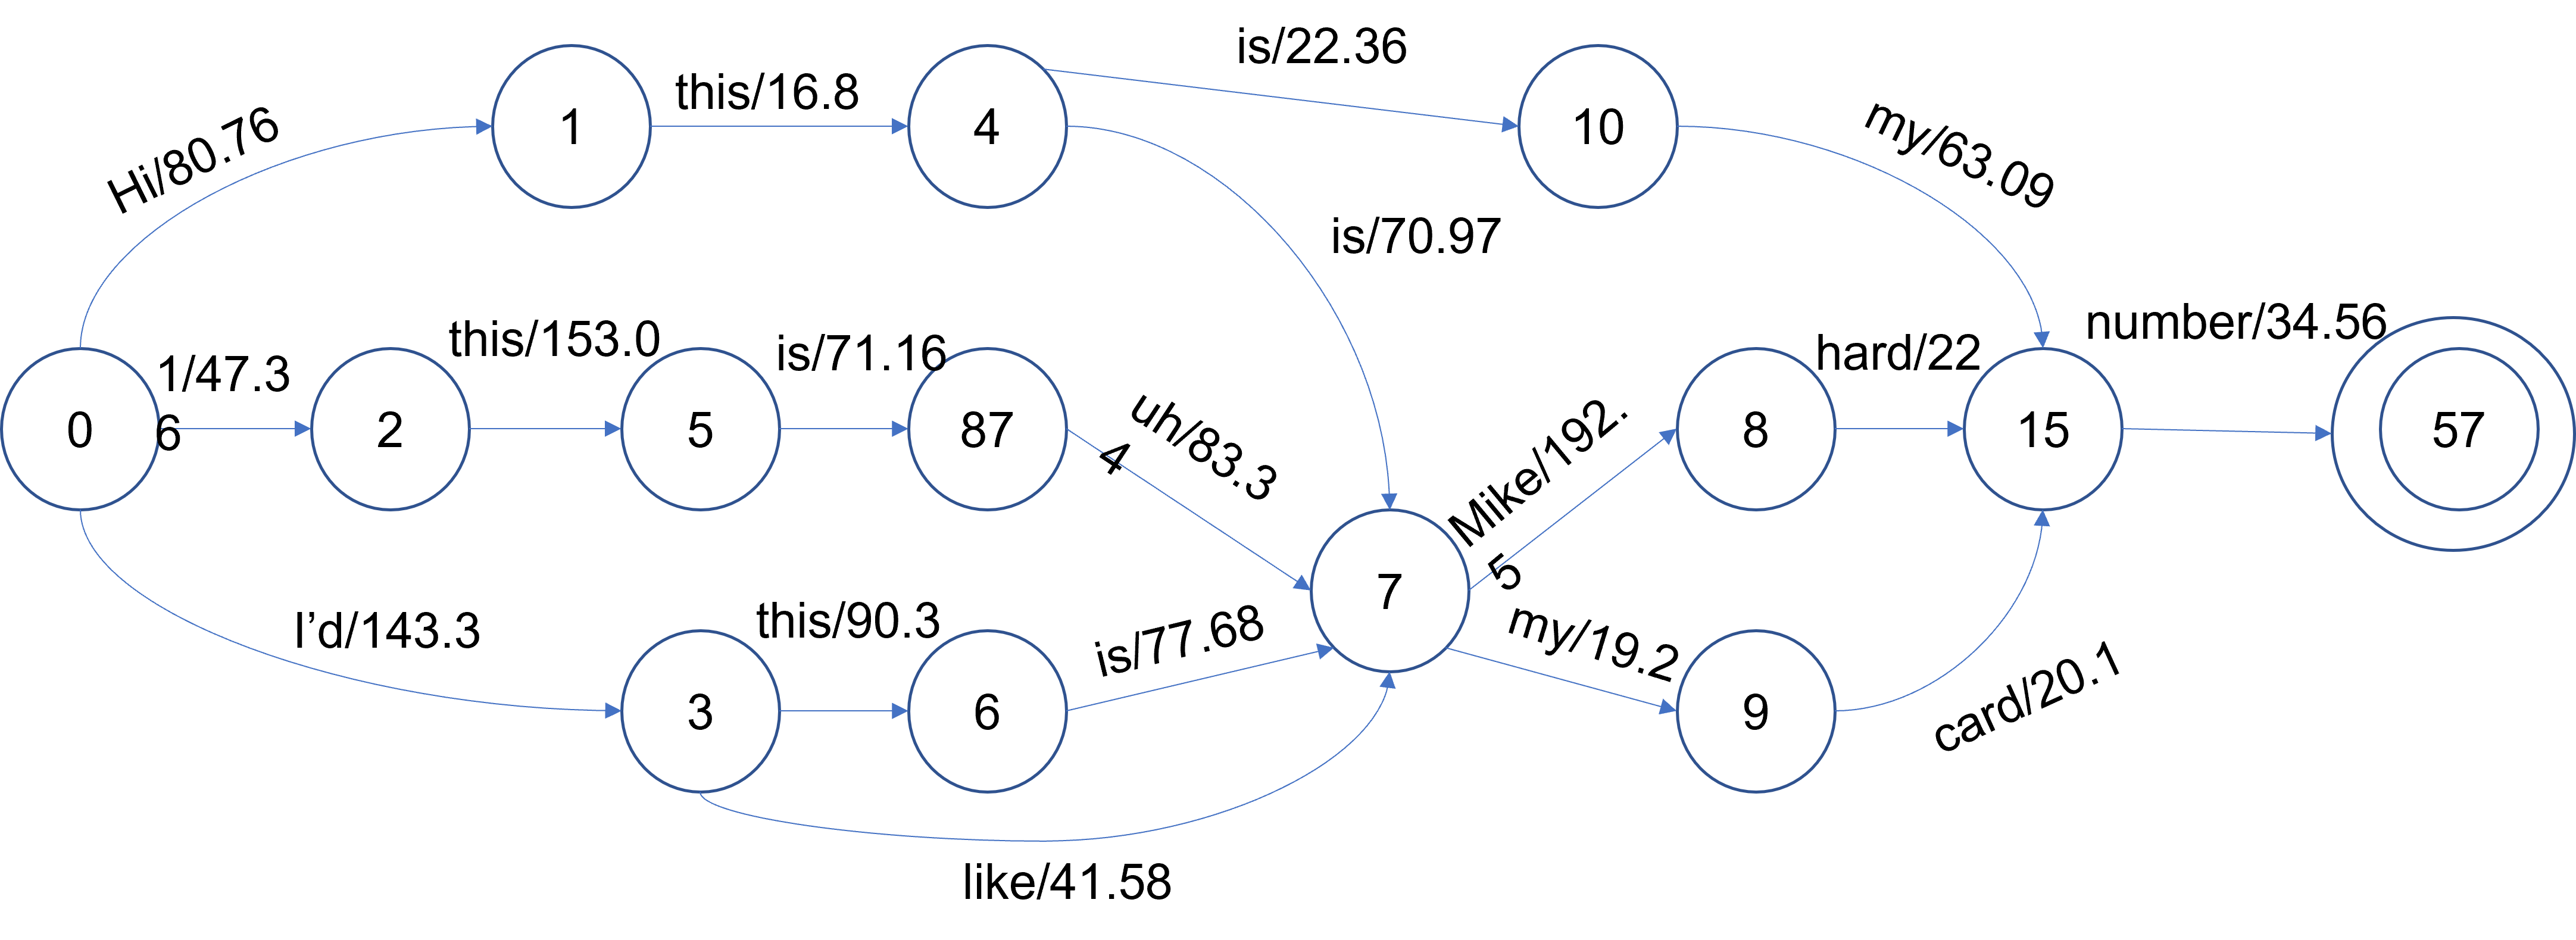
\includegraphics[width=0.9\textwidth]{img/LatticsMMI.png}
    \caption{Lattice formation}
    \label{fig:Lattice formation}
\end{figure}

Lattice-based methods were proposed prior to GPU era. It is not possible to train this deep network without a GPU but with Deep Learning in 2012 on GPUs, new possibilities emerged but the physical limitations, particularly, memory consumption problem remained. To fit the method into the GPU's memory, for example, we chop the training utterances into 1 to 1.5 second chunks which is not enough. GPU allows one GPU instruction to be run on multiple data sets one at a time. We must avoid branching to get the most benefit out of the GPU and pruned tree search does not seem so appealing with GPU which is why a smaller model is required \cite{povey_purely_2016}.

\subsection{Bypassing Lattices through Chain Model for \\ Improving Efficiency}
With the advent of E2E models, the need of a trained system for lattice initialization became a disadvantage of lattice-based MMI. Hence, comes the concept of Lattice Free MMI \cite{povey_purely_2016, ghahremani_investigation_2017} which is purely sequence trained requiring no no cross-entropy training as it does not use a lattice allowing it to exactly compute the sum instead of just approximating it \cite{noauthor_lattice_nodate}. The LF-MMI objective function is the modified form of MMI discriminative  objective function which enables ASR Training on GPU in HMM-DNN ASR Approach. 

The \textit{chain} or LFMMI models are a different form of HMM-DNN model. It uses Neural Networks \cite{daniel_povey_kaldi_nodate} which are a different point of design in the space of acoustic models compared to Traditional ASR models. It uses a three times smaller frame rate at the Neural Network output which reduces the computational requirements significantly in test-time, making decoding in real-time  much simpler. 

\begin{figure}[h]
    \centering
    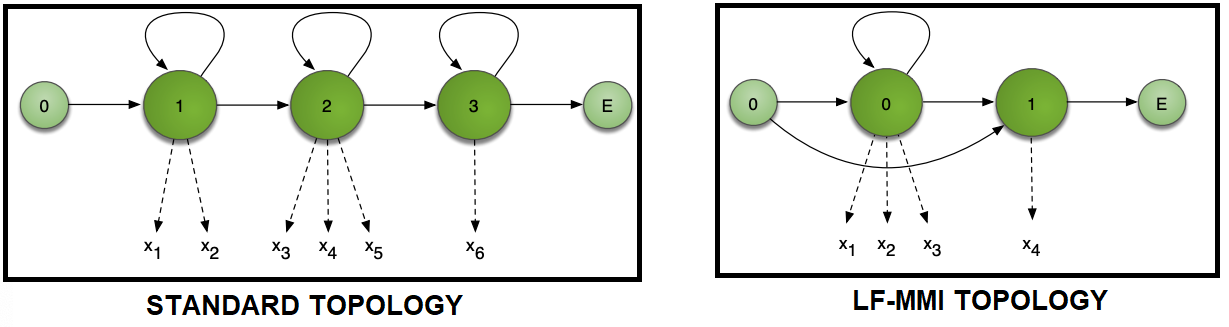
\includegraphics[width=0.8\textwidth]{img/LFMMI1.png}
    \caption{Standard vs LF-MMI Topology}
    \label{fig:LFMMI-topology}
\end{figure}

Due to the reduced frame rate, unconventional HMM topologies must be used to enable one-state HMM traversal. The chain model employs HMM's fixed transition probabilities but does not train it actually. Neural-net output probabilities can typically serve the same purpose as transition probabilities depending on the topology \cite{daniel_povey_kaldi_nodate}.

Models are trained with a sequence-level objective function, i.e. the log-probability of the correct sequence, from the start. It is implemented in an MMI-based system without lattices on GPU by performing a complete forward-backward computation on a decoding graph derived from a phone-based n-gram language model \cite{povey_purely_2016}. 

\begin{figure}[h]
    \centering
    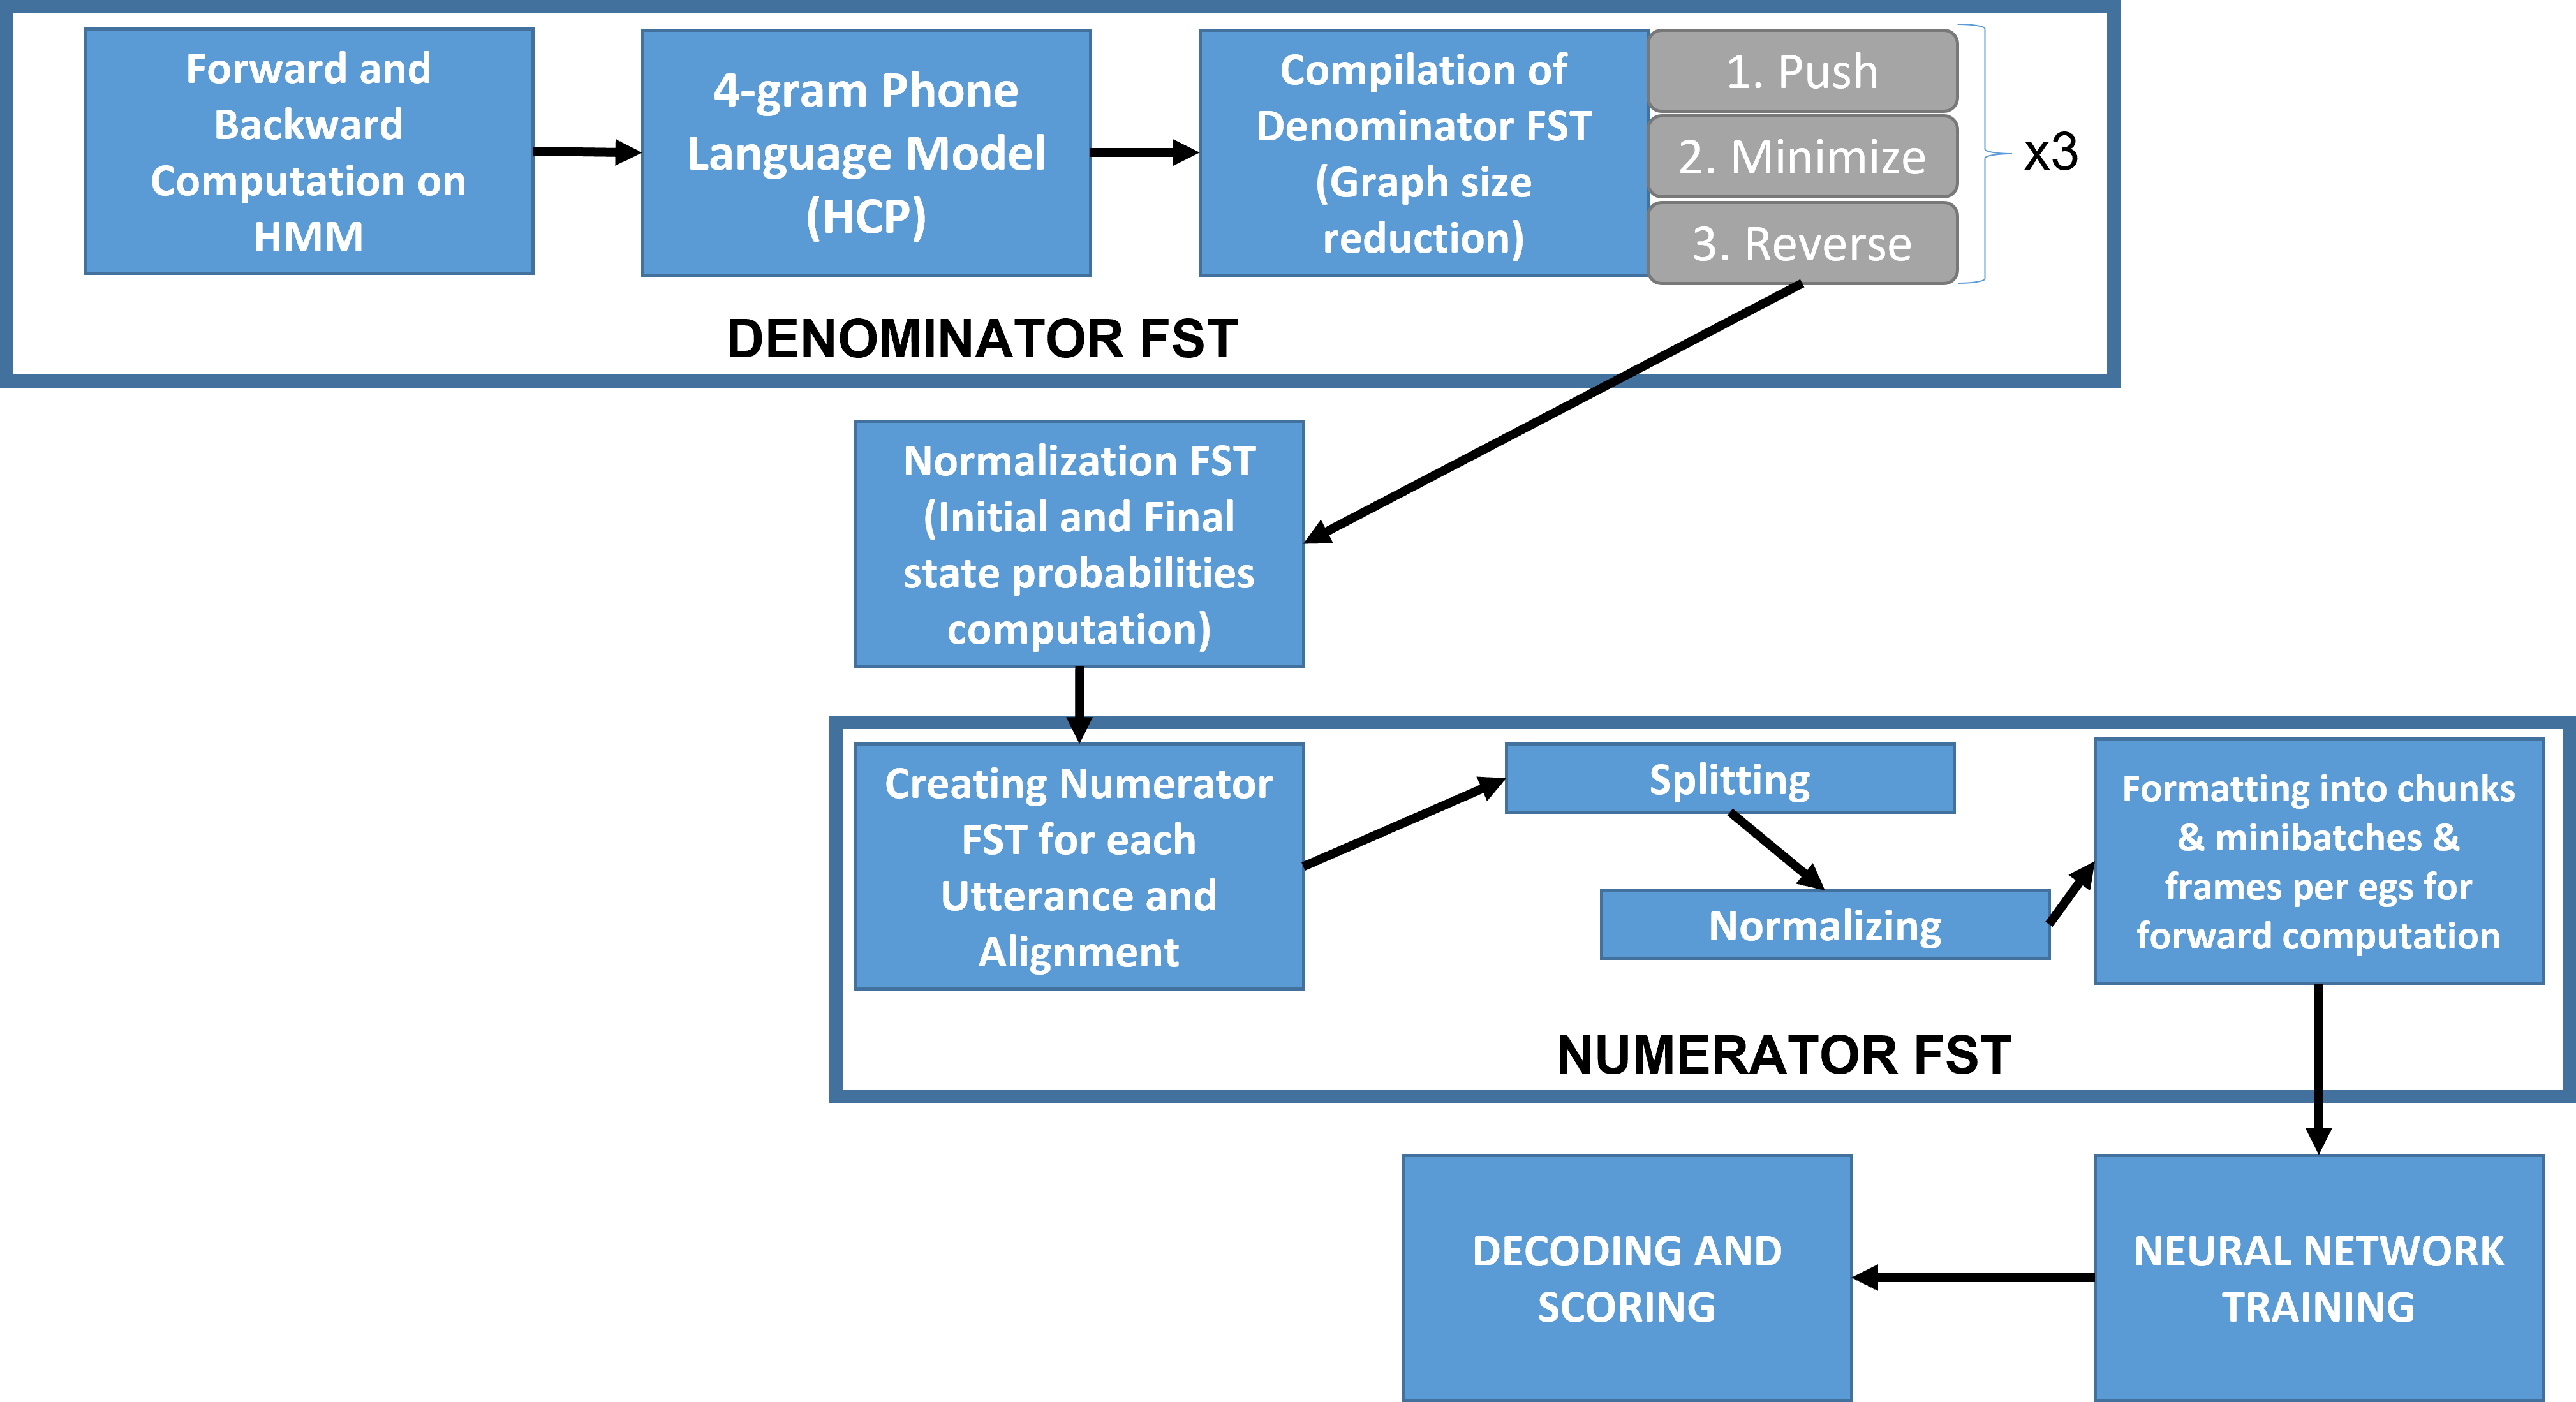
\includegraphics[width=0.9\textwidth]{img/ChainTrg.png}
    \caption{Chain Model Overview}
    \label{fig:chain-overview}
\end{figure}

%https://slideplayer.com/slide/17724439/
%https://jonathan-hui.medium.com/speech-recognition-maximum-mutual-information-estimation-mmie-a0db565764aa

If the denominator is represented as a graph and it is fitted in the GPU allowing computations to be efficiently performed for which following modifications are done \cite{noauthor_lattice_nodate, wiesner_lattice_2020}:

\begin{enumerate}
    \item Using Phone LM instead of Word-based LM to reduce size of graph significantly because there are far fewer possible phones than there are words.
    \item There are three times fewer outputs for any utterance to compute because DNN outputs are computed at a third of the standard frame-rate \cite{povey_purely_2016} which is done by decreasing the frame-shift to 30ms from traditional 10ms which means that the standard 3-state left-to-right HMM topology, commonly used in ASR, cannot be used since the entire HMM is required to be traversed in a single frame. Training such a system using the MMI objective requires the objective and its derivative to be computed effectively. 
    
\end{enumerate}

We have very limited transcribed data available for training purposes but we do have a huge amount of Call Center Data available. If we only have only a small amount of data transcribed, but much more un-transcribed data best is to train a seed model and use it to transcribe more data. But also don't want to train further on incorrect captions. So we apply data filtering based on confidence scores to select out the harder data that is most useful for refining the system. One of the solutions can be \cite{ghahremani_investigation_2017} to use a lattice to incorporate uncertainty about the transcription, and train with the LF-MMI criterion but that requires a strong language model for the best performance\cite{wallington_learning_2021}.

LF-MMI has shown to achieve better performance on various data-sets like Aspire using various different HMM-DNN and E2E ASR frameworks \cite{ghahremani_investigation_2017, tian_consistent_2022} compared to lattice based MMI model.







    %!TEX root = ../thesis.tex
\chapter{Literature Review} % (fold)
\label{cha:literature_review}

Due to limited work and constraint of availability of relevant literature with regards to our scenario we took a 3-part approach to our literature i.e.
\begin{itemize}
    \item Literature on ASR in English Language.
    \item Literature on Languages relevant to Urdu i.e. Arabic and Hindi.
    \item Literature specific to ASR implementation in Urdu Language - A low resourced language.
\end{itemize}

\section{Literature on English Language}

There is ample amount of literature on English ASR available. In fact all state-of-the-art Training methods from Traditional ASR to Hybrid HMM-DNN to modern E2E Systems are thoroughly tested on English Language with WERs $<6\%$. 

\cite{dahl_context-dependent_2012} first introduced HMM–DNN hybrid approach in which Deep neural network model replaced GMM which increased accuracy compared to traditional HMM-GMM legacy system. They achieved 5.8\% and 9.2\% absolute sentence accuracy improvement or 16.0\% and 23.2\% relative error reduction over the CD-GMM-HMMs trained respectively using the minimum phone error rate (MPER) and maximum-likelihood (ML) criterion on Bing Voice Search Business English Dataset with 24 hours of training set (32057 utterances), 6.5 hours of Dev Set (8777 utterances) and 9.5 hours of Test Set (12758 utterances). The data-set had variations like noise, music, side-speech, accents, sloppy pronunciation, hesitation, repetition, interruption, and different audio channels. This however would require us to build our own code-switched Language model based on our own corpus.

\cite{georgescu_performance_2021} studied and compared the performance of Hybrid HMM-DNN and Deep Learning based methods trained on English LibriSpeech data-set of 1000hours, which showed that Hybrid HMM-DNN based systems, particularly TDNN and CNN-TDNN outperformed End to End Methods with WER of 3.85\% and 3.87\% respectively with least memory load of 106 MB for loading NN model and storing all the activation's of the network for processing per second of speech which supports the conclusion by \cite{christian_gaida_comparing_2014} and \cite{naeem_subspace_2020}. This model was however not trained on noisy telephonic data which is why it is not applicable for our scenario. Moreover, it was trained only on English and our language modelling would different and irrelevant for our code-switched Urdu scenario.  

\cite{smit_advances_2021} implemented sub-word units in using DNN based acoustic and RNN based language models trained on on 283 hours of English Data-set which resulted in WER of 18\% which was too high for our use. 

\section{Literature on Languages relevant to Urdu i.e. Arabic and Hindi}
For greater insights, we selected two of the languages that were closest in structure (written and spoken) to Urdu Language; Arabic and Hindi. There was ample amount of research available in these languages which helped cover up for the shortcomings in the research pertaining to Urdu ASR, particularly the code-switched version.

\subsection{Arabic Language}
Arabic is one of the most actively researched language in ASR field. \cite{khurana_qcri_2016} merged three acoustic models trained with LFMMI objective function using similar architecture as \cite{povey_purely_2016} on 1200 hours of Dialectical Arabic MGB-2 data-set. They merged TDNN, LSTM, and BLSTM using the Minimum Bayes Risk decoding criterion, achieving WER of 14.2\%. 

Ali Et al (2017) from Aalto University \cite{ali_speech_2017} merged 30-plus systems using MBR, including two acoustic models TDNN-BLSTM along with variety of language models like character-based, sub-word, and word-based \cite{smit_aalto_2017}. 13.2\% WER was achieved on MGB-2 which was a 10\% improvement compared to results of 2016, and 37.5\% average WER and 29.3\% multi-reference WER was achieved on MGB-3. These were based on Arabic language and not applicable for our uses. Moreover, Arabic is far more resourceful compared to Urdu which is why we could not use this for our Code-Switched Urdu environment. 

\cite{alsayadi_arabic_2021} conducted training of Models in Traditional ASR and E2E ASR using 1200 hours of Arabic Speech Corpus \cite{alhanai_development_2016}.
Eight models for traditional ASR have been used, four of which use GMM, two of which use SGMM, and the last two models use DNN. End-to-end methods for diacriticised Arabic ASR were used which are based on CTC-attention and CNN-LSTM. WER of 33.72\% on conventional ASR and 28.5\% on CNN-LSTM. The drawback of this for our case was that training a model like this needed 1000 of hours of labelled data for training and that volume of labelled code-switched Urdu data was not available to us.

\cite{hussein_arabic_2022} comprehensively performed  bench-marking for E2E transformer, modular HMM–DNN, and human speech recognition on the Dialectical Arabic. End-to-end ASR gave 12.5\%, 27.5\% , 33.8\% WER on MGB-2, MGB-3, and MGB-5 data-sets respectively. The drawback is that we did not have labelled data for code-switched Urdu to conduct this kind modelling. %Their results also showed that human performance in the Arabic language is still considerably better than the machine with an absolute WER gap of 3.5\% on average.

\begin{figure}[h!]
    \centering
    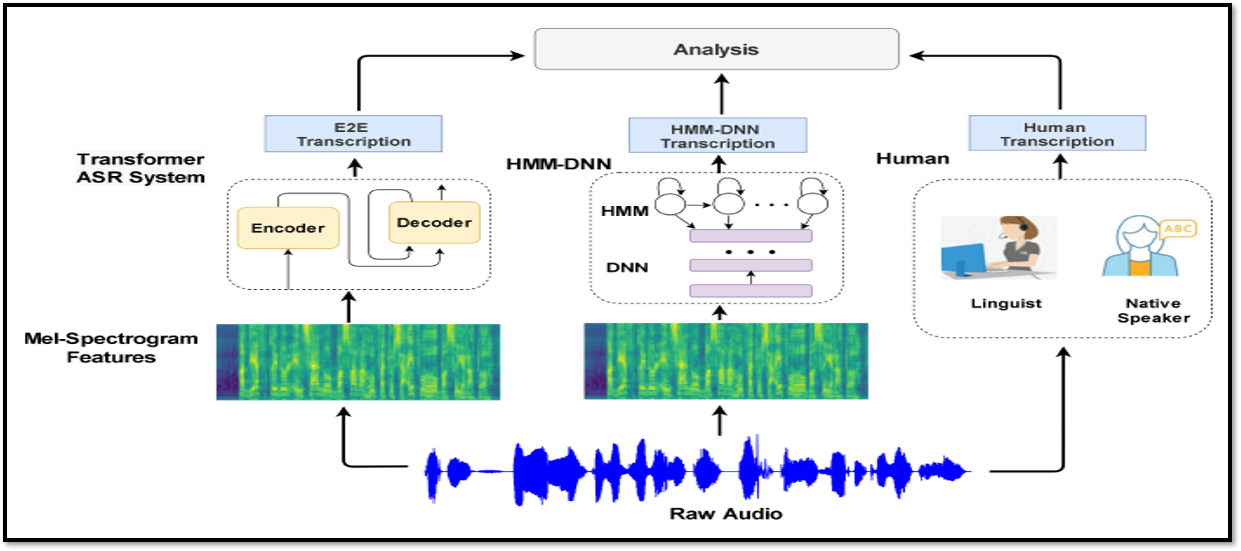
\includegraphics[scale=0.40]{img/ASR-diagram-comparison.png}
    \caption{E2E vs Hybrid DNN-HMM vs HSR \cite{hussein_arabic_2022}}
    \label{fig:hybrid-vs-e2e-HSR}
\end{figure}

\subsection{Hindi Language}
The majority of work in the field of speech recognition in South Asian Languages has been done on Hindi, which is very similar to spoken Urdu \cite{farooq_improving_2019} \cite{dash_automatic_2018}. Isolated word recognition \cite{patil_automatic_2016}, connected digit recognition \cite{a_n_mishra_robust_2011}, statistical pattern classification \cite{aggarwal_using_2011}, online speech to text engine \cite{b_venkataraman_sopc-based_2006} and large vocabulary speech recognition systems have been developed in Hindi \cite{kumar_large-vocabulary_2004}. 

On the AMUAV Hindi speech database, Upadhyaya \cite{tanveer_continuous_2019} developed a Hindi speech recognition system using deep neural networks. This database contains 1000 phonetically balanced sentences recorded by 100 different speakers and covers 54 different Hindi phones. Using DNN implementation by \cite{karel_vesel_sequence-discriminative_2013}, the minimum achieved WER was 11.63\% which is high for our use.

Lakhshmi's \cite{lakshmi_sri_kaldi_2020} work involved training a data-set of 158 Hindi medical terms from 16 female and 11 male speakers, almost 3 hours of data, audio sampled at 16KHz, single channel. Best WER of 2\% was achieved using Triphone Acoustic Modelling. Although this system has a low WER, it cannot be used as a replacement for Urdu ASRs due to significant differences in lexicon, pronunciations etc \cite{k_v_s_parsad_and_s_m_virk_computational_2012}.

In general, using Hindi Language Model is not the optimum solution to implement in Code-switched Urdu telephonic environment due to differences in the linguistic foundation, vocabulary, written scripts, etc which means that using Roman Hindi model for Speech to Text will not be optimal because of differences in writing and pronunciation of words e.g. the word \textit{"Zeera"} in Urdu is pronounced \textit{"Jeera"} in Hindi (in writing and in pronunciation both). Phones like \textit{"/Z/"} \textit{"/kh/"} \textit{"/gh/"} are pronounced differently in Hindi and in Urdu. This will result in low accuracy in our scenario.

\section{Literature on Urdu Language}

Urdu has about 170 million speakers \cite{ethnologue_urdu_nodate} and is spoken in India, Pakistan, Bangladesh, and many other parts of the world which is why it is important that the benefits of ASR are available in the Urdu domain. Urdu is low resourced due to scare publicly available text corpus, transcribed speech data and pronunciation lexicon. A robust ASR generally requires thousands of hours of transcribed speech data, as well as a massive text corpus and lexicon. As a result, Urdu speakers are excluded from the benefits of ASR. 

Over the years, very little efforts have been made to develop resources and speech-technology-related applications for Urdu compared to English and Arabic. Ashraf et al. 2010 \cite{hutchison_speaker_2010} pioneered the development of an isolated speech recognition system in the domain of Urdu speech recognition. The vocabulary comprised of 52 words spoken by 10 speakers. For unseen speakers, a minimum Word Error Rate (WER) of 10.6\% was achieved. This was done on limited vocabulary and has high error rate which is why it is not applicable for our use and was only tested on isolated words whereas we needed a LVCSR.

\cite{sarfraz_large_2010} developed a continuous speech recognition system in Urdu using spontaneous speech corpus collected from 82 speakers which had WER of 68.8\%. \cite{sarfraz_huda_speech_2016} recorded the speech corpus over telephone and microphone channels. The corpus duration was 45 hours, with vocabulary of 14000 words. A minimum WER of 68.8\% was attained which was too high for our use.

A speaker-independent Urdu speech recognition system was developed by Qasim \cite{qasim_urdu_2016} for 139 district names of Pakistan which covered various Pakistani accents, giving WER of 7.44\% by building adapted ASR on field data. This is not applicable for our use because it has a limited vocabulary and would not work in a noisy code-switched Urdu environment. 

Shaikh et al 2015 \cite{shaik_improvements_2015} developed an LVCSR on 99 hours of Urdu broadcast data with vocabulary of 79,000 words. A 5-gram Language Model was built with corpus of 266 Million words collected from various newspapers. Evaluation was done on 0.5 hours of data which gave WER of 32.6\% using GMM-HMM based speaker adapted system. The data set and model however is not openly available and the word error rate is too high for our use. Moreover, GMMs has a drawback of being inefficient for nonlinear class boundaries because they assume each frame is generated by a single component of the mixture which required them to be replaced by DNNs \cite{dahl_context-dependent_2012}.

Raza \cite{raza_rapid_2018} collected 1207 hours of speech dataset from 11017 speakers all over Pakistan with vocabulary of 5000 words from which 9.5 hours data was annotated and out of that, 8.5 hours were used as training dataset. Evaluation was done on 1 hour of test data which gave WER of 24.14\% which was too high for our use. 

\cite{farooq_improving_2019} developed an LVCSR using 300 hours of read-out speech data, in both indoor and outdoor environments, with a vocabulary size of 199,000 words from 1671 Urdu and Punjabi speakers. GMM-HMM, TDNN, LSTM, and Bidirectional  LSTM based Acoustic Modelling is done. For re-scoring, Recurrent Neural Network Language Model (RNNLM) was used. Evaluation was done on 9.5 hours of test data-set giving WER of 13.5\% which was too high for our use.

\cite{farooq_enhancing_2020} used 25 hours of their own Urdu speech corpus for enhancement of read-Urdu-speech LVCSR to recognize code-switched speech using the HMM-DNN modeling technique without any prior GMM-HMM training and alignments. Various techniques to improve language models using monolingual data were used giving overall percent Word Error Rate (WER) 26.95\%.

\cite{naeem_subspace_2020} developed SGMM based ASR model for continuous speech with the Data-set structured by RUMI, CSALT and FAST-NUCES. They developed a 50-hour Urdu speech data set, transcribed and merged with CSALT, ITU data-set to produce 100 hours of audio data-set. Audio files had sampling rate of 16000Hz and used mono-channel. They achieved a WER of 9.7\% with 100 hours of their data. The drawback is that data as well as the model is however not openly available and it is not tested in a telephonic audio data. 
 
Sehar Gul \cite{sehar_gul_detecting_2020} developed an ASR to detect malicious speech using Deep Speech \cite{mozilla_deep_nodate} (an End to-End ASR Engine) with 86 malicious sentences, 100 random Urdu sentences, and 250 sentences from Ali et. al 2015 \cite{ali_automatic_2015} spoken by 10 speakers, sampled at 8K mono channel. It achieved a Word Error Rate of 40\%. The drawbacks are that it was trained on Deep Learning platform with very less dataset. It was also not applicable on a noisy environment which required us to redesign the whole Speech To Text Pipeline.   

\cite{qureshi_urdu_2021} trained an ASR with the PRUS data-set  \cite{zia_pronouncur_2018} comprising of 708 sentences by 7 speakers with GMM based triphone acoustic models which gave overall recognition accuracy values 78.2\% for 100 words. This was a good baseline for us to work with since that data was available to us. %First five experiments were trained a GMM based tri-phone acoustic model on the first 600 sentences of the corpus. Sixth experiment was trained a GMM based tri-phone acoustic model on the first 600 sentences of each speakers’ corpus (combined first 600 sentences of each member to form one large training corpus) and tested it on the rest of the 108 sentences of each speaker’s corpus (combined 108 sentences of each member to form one testing corpus). Experiment 7-11 trained a GMM based tri-phone acoustic model on the complete corpus (708 sentences) of n-1 speakers and tested it on the complete corpus of the remaining 1 speaker, so 5 different models (leaving out SP1-SP5).

While the work mentioned in the preceding literature reports achievements on the Urdu ASR task, it lacks information on free corpus and does not point out corpus resources that others could adopt and use for a fair comparison. We used data-set from Ali et al 2015 \cite{ali_automatic_2015}, Sehar \cite{sehar_gul_detecting_2020} and PRUS \cite{zia_pronouncur_2018} \cite{qureshi_urdu_2021} results of which were compared with our model (\ref{sec:comparison_result}).

\section{Challenges} % (fold)
\label{sec:challenges}
Based on our literature review, we will need to build our own ASR from scratch because of lack of availability of good pre-trained models and data-sets in Urdu language for Noisy Telephonic Environment, with good WER and SER. In this regard we need:
\begin{itemize}
    \item ASR training model to train our data   
    \item Telephonic code-switched Urdu audio data-set (Mono 16000Hz) with Roman Urdu Transcript which would cater for:
    \begin{itemize}
        \item Isolated Digits
        \item Isolated words
        \item Read Speech (Words and Digits)
        \item Spontaneous Speech (Words and Digits)
        \item Clean Audio
        \item Noisy or Telephonic Audio
    \end{itemize}
    %\item Practical Implementation setup for testing our work. 
    \item Achievement of WER $<$ 10\% and SER $<$ 30\% in clean as well as in noisy environment (as well as in spontaneous, read-speech and isolated words)
\end{itemize}

%\begin{figure}[h!]
%    \centering
%    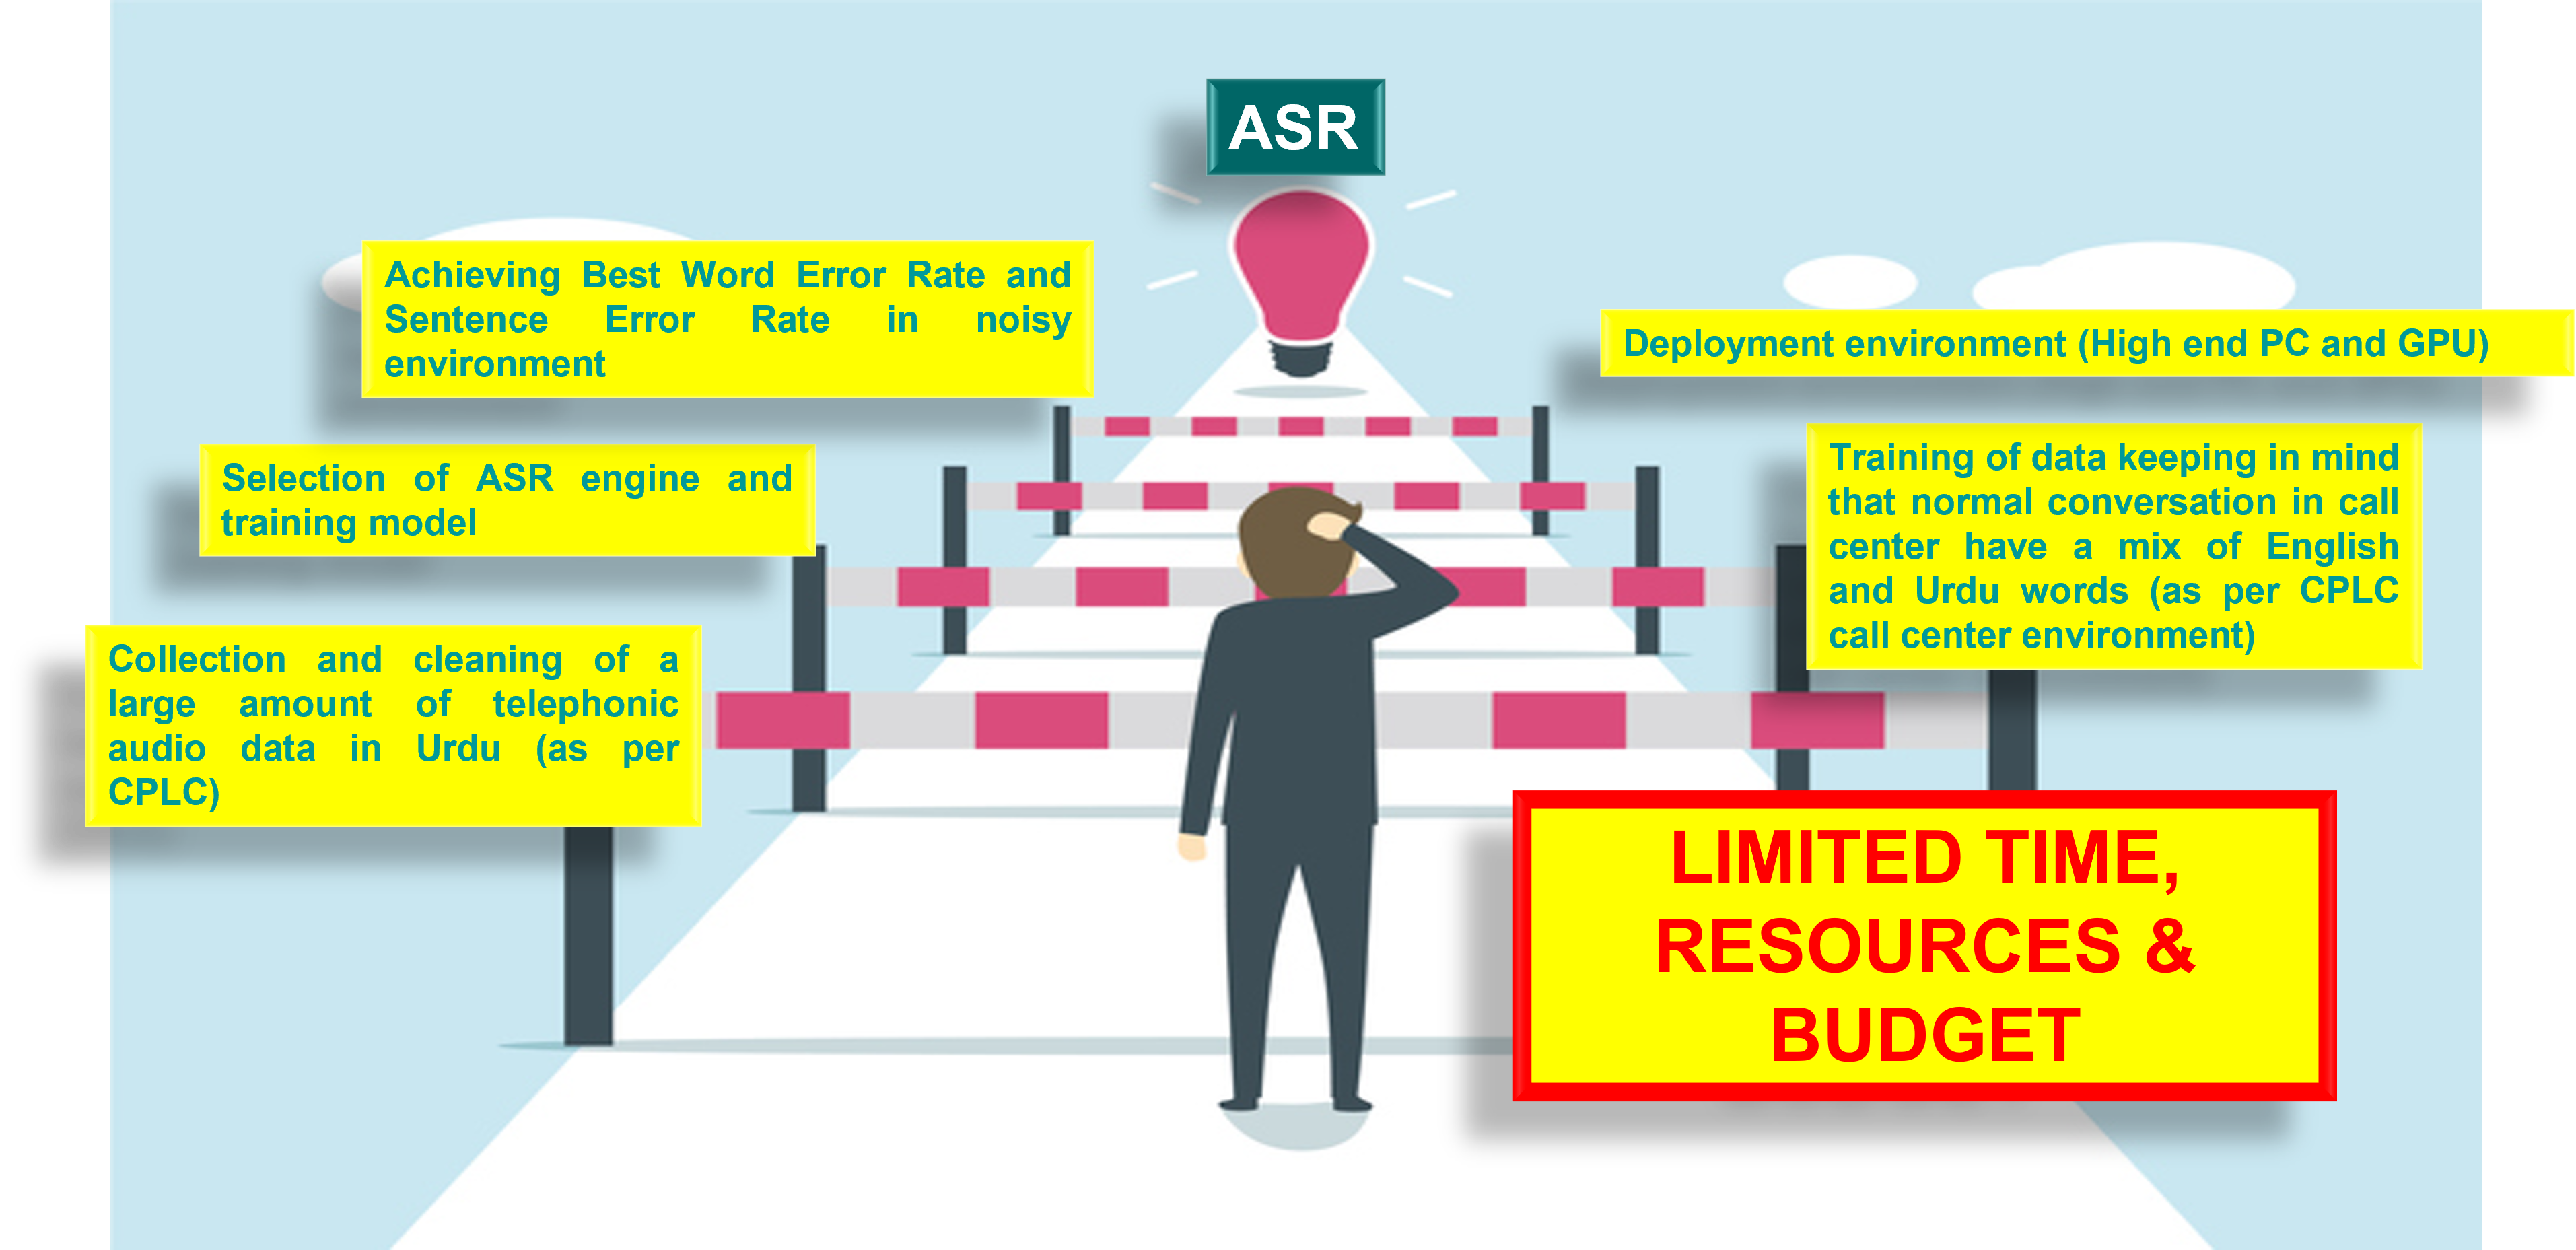
\includegraphics[scale=0.5]{img/Challenges.png}
%    \caption{Challenges to our work}
%    \label{fig:challenges}
%\end{figure}

\section{Selection of Approach for our Methodology}
The majority of AI applications are currently model-centric, a possible reason being that AI industry pays close attention to academic research on models. Since it is difficult to create large data-sets which can become widely accepted standards, more than 90\% of AI research papers are model-centric \cite{deeplearningai_data-centric_2021}. The Code becomes the major focus and data-set is frequently overlooked which is why data collection and pre-processing is considered as a one-time event.

Accenture \cite{noauthor_scaling_nodate} informs that about 85\% of projects are still proof of concept \cite{noauthor_data-centric_nodate} which are not brought into production, yet. The reason why model-centric approach of previous works have not been deployed in production environment include:

\begin{enumerate}
    \item \textbf{Requirement of highly customized solutions.} 
    \begin{itemize}
        \item Various companies e.g. manufacturing company with multiple line of products cannot apply one Model for all products to detect production errors in them, unlike advertisement companies like Google or facebook Ads.
        \item In ASR scenario, model for one language cannot work on all languages because every language needs different model. Giants like Google, Microsoft or Facebook may be able to have ML department for each product line but not every company can afford the cost of Data Scientists/ Engineers and MLOps Engineers.
    \end{itemize}
    \item \textbf{Limited points of Data Collection.} 
    \begin{itemize} 
        \item Every industry does-not have multiple data sources or data points. Sometimes, the available data-set itself is small e.g. in cases of a small textile fashion brand or a call center solution with limited calls. 
        \item Not all businesses have an effective data collection and standardisation pipeline. If their ML solution is overly model-centric, they will be necessitated to work with small data-sets (i.e. $102$ - $103$ relevant data points), which are known for producing unsatisfactory results for production standards.      
    \end{itemize}
    \item \textbf{Proof of Concept vs Actual Software Deployed in Production.} There are various types of research claiming things that are not actually deployed in a real-world scenario like in 2019, it was published \cite{ardila_end--end_2019} that certain solutions were developed to accurately detect tumours at an earlier stage than trained radiologists are able to diagnose. The reason this model is not in every hospital yet is due to a substantial gap between the proof of concept and hospital production software. 
\end{enumerate}

Hence, we utilized a more data-centric approach towards ASR. We decided to take a small set of quality data and train an accurate model on it which will be used to annotate remaining data set. The data-set will then be audited and improved to build a golden data set which can then be used to deploy Machine Learning algorithms to train the most accurate model on a Larger Vocabulary set. Hence we decided to use Hybrid HMM-DNN method of training ASR which takes relatively less time than Deep Learning while yielding best results. 

\begin{figure}[htb]
    \centering
    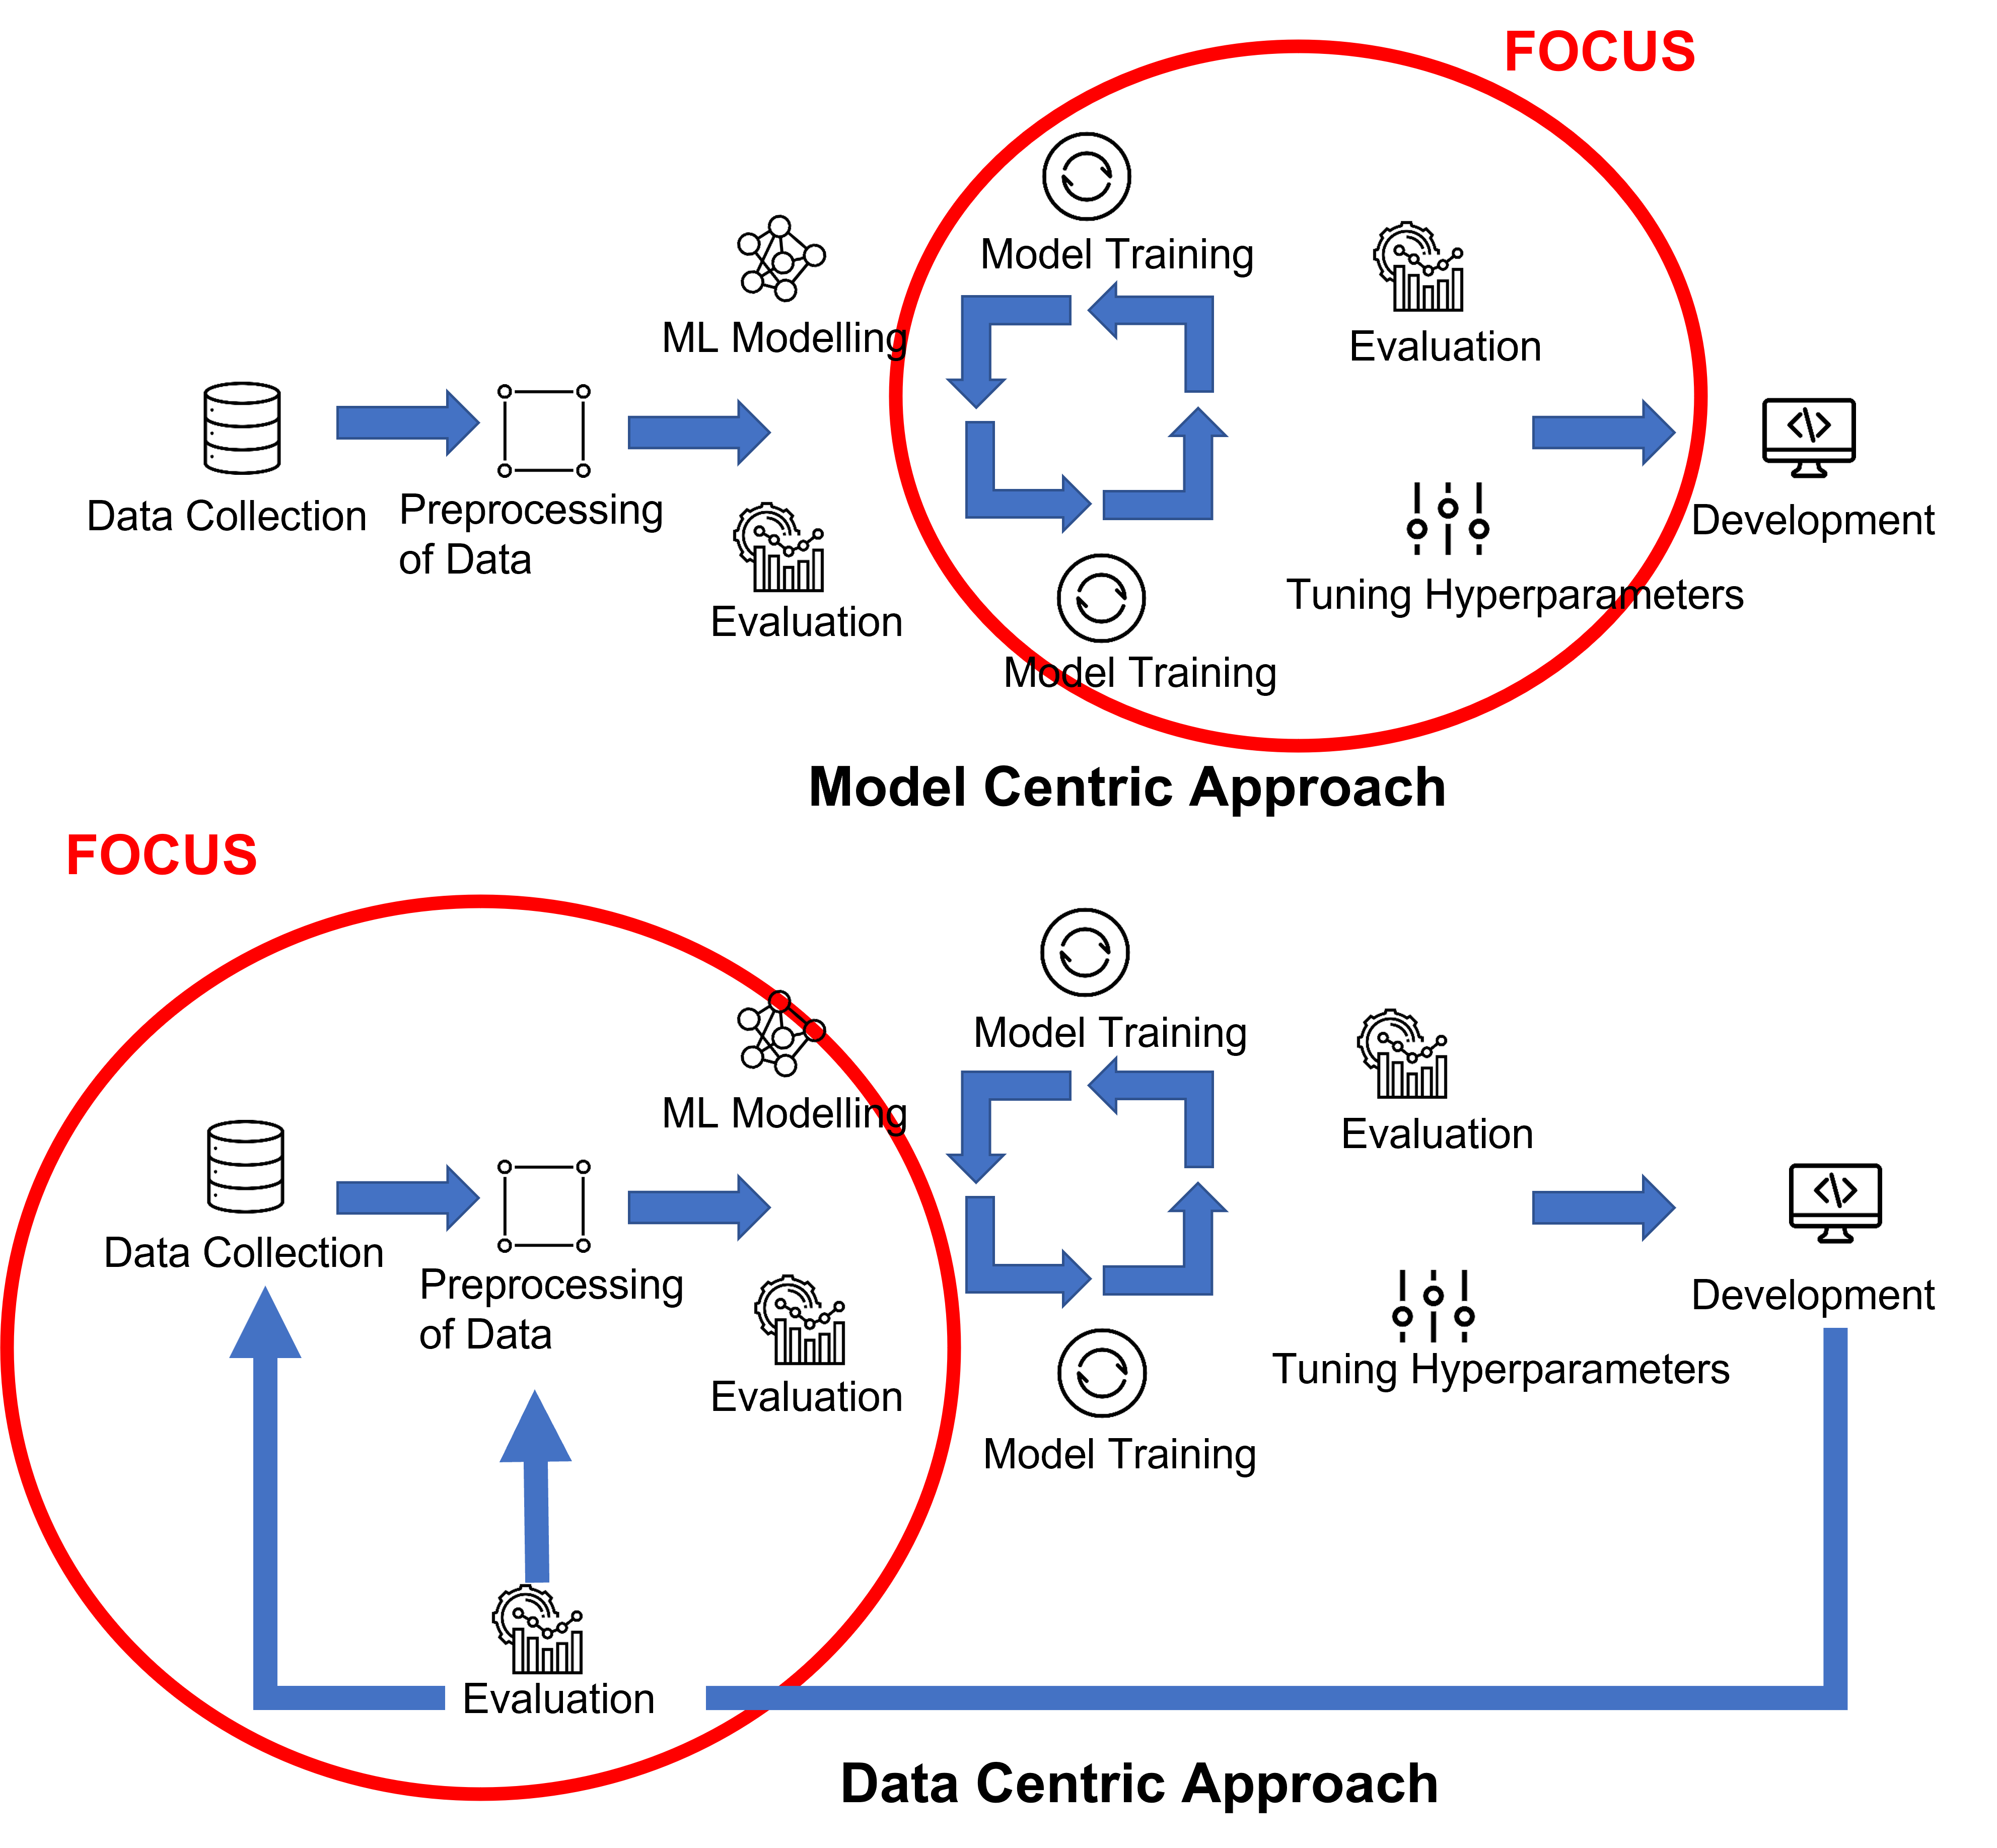
\includegraphics[width=0.7\textwidth]{img/datacentervsmlcenter - 2.png}
    \caption{Data-Centric Vs Model-Centric Approach}
    \label{fig:datacent-vs-modelcent}
\end{figure}

In the implementation of data-centric approach following steps are important \cite{radecic_data-centric_2022}:
\begin{enumerate}
    \item \textbf{Iterative Collection of Data} - Data collection is an iterative process in a data-centric approach, particularly for companies that do not have millions of data points or sources, thus, improving the performance of AI systems as well as the quality and quantity of data.
    \item \textbf{Iterative evaluations} for Data Drift Detection  
    \item \textbf{Quality Data Labelling:} Labelling is often done manually which means human errors and biases will exist. If there are inconsistencies w.r.t how the human experts approach particular problem, machines are not likely to detect those inconsistencies. For this we need to ensure that: 
    \begin{enumerate}[label=(\alph*)]
        %\item \textbf{Multiple labelers, editors and auditors to spot inconsistencies}  
        \item Labelling instructions to be defined and the process to be improved with time and implemented accordingly. 
        \item Inclusion of domain knowledge and expertise.
        \item Maintaining Control of labelling annotation process.
    \end{enumerate}
    \item \textbf{Data Augmentation} - It describes techniques for increasing the number of data points in your sample or the number of defective production parts, by \textit{generating the unseen data} that your model has not seen during the training time and \textit{Removing or adding the noisy observations for adding variance}. We also played around with the speed of data, make changes to pitch or tone, length, adding silences or extra noises using audio editing tools \cite{noauthor_linux_nodate} which added variety.        
\end{enumerate}

Based on above, we decided to take a more Data-Centric Approach where our focus is on making quality Data-set instead of Model Centric approach to Machine Learning as shown in Figure \ref{fig:datacent-vs-modelcent}.






    %!TEX root = ../thesis.tex
\chapter{Our Work} % (fold)
\label{cha:our_work}

In this chapter we will discuss our methodology to build a Code-switched Urdu ASR from scratch.

\section{Proposed Methodology}

We proposed a \textit{"Data Centric Approach with Hybrid HMM-DNN ASR Training method using LFMMI CNN-TDNN for building a Code-switched Urdu ASR"}. The data-centric involved focusing on Data Preparation primarily, leading to better input for the machine learning process because ASR model quality cannot out perform its data quality. We used alot of diversity in our data-set to cater for various scenarios like isolated digits and alphabets, continuous speech etc in clean and noisy backgrounds. The learning model we used is a hybrid HMM-DNN in which we use HMM based state posteriors and train Neural Network i.e. CNN-TDNN with LFMMI objective function.

Figure \ref{fig:working_pipeline} shows our designed workflow to train and deploy our ASR. The main steps of Data Pre-Processing, Language Modelling, Feature Extraction, Acoustic Modelling, Analysis and Output are linked by red lines and shown as dashed blue outlines. The internal workings within the steps are shown by blue filled boxes with blue arrows. Any internal process that is linked to internal process of another is shown by Orange arrows. The three parts of Acoustic training i.e. Monophone, Triphone and Neural network training are shown within acoustic modelling as green dotted line boxes and their internal working are shown as blue filled boxes linked with blue arrows.

\begin{landscape}
    \begin{figure}[htb]
    \centering
    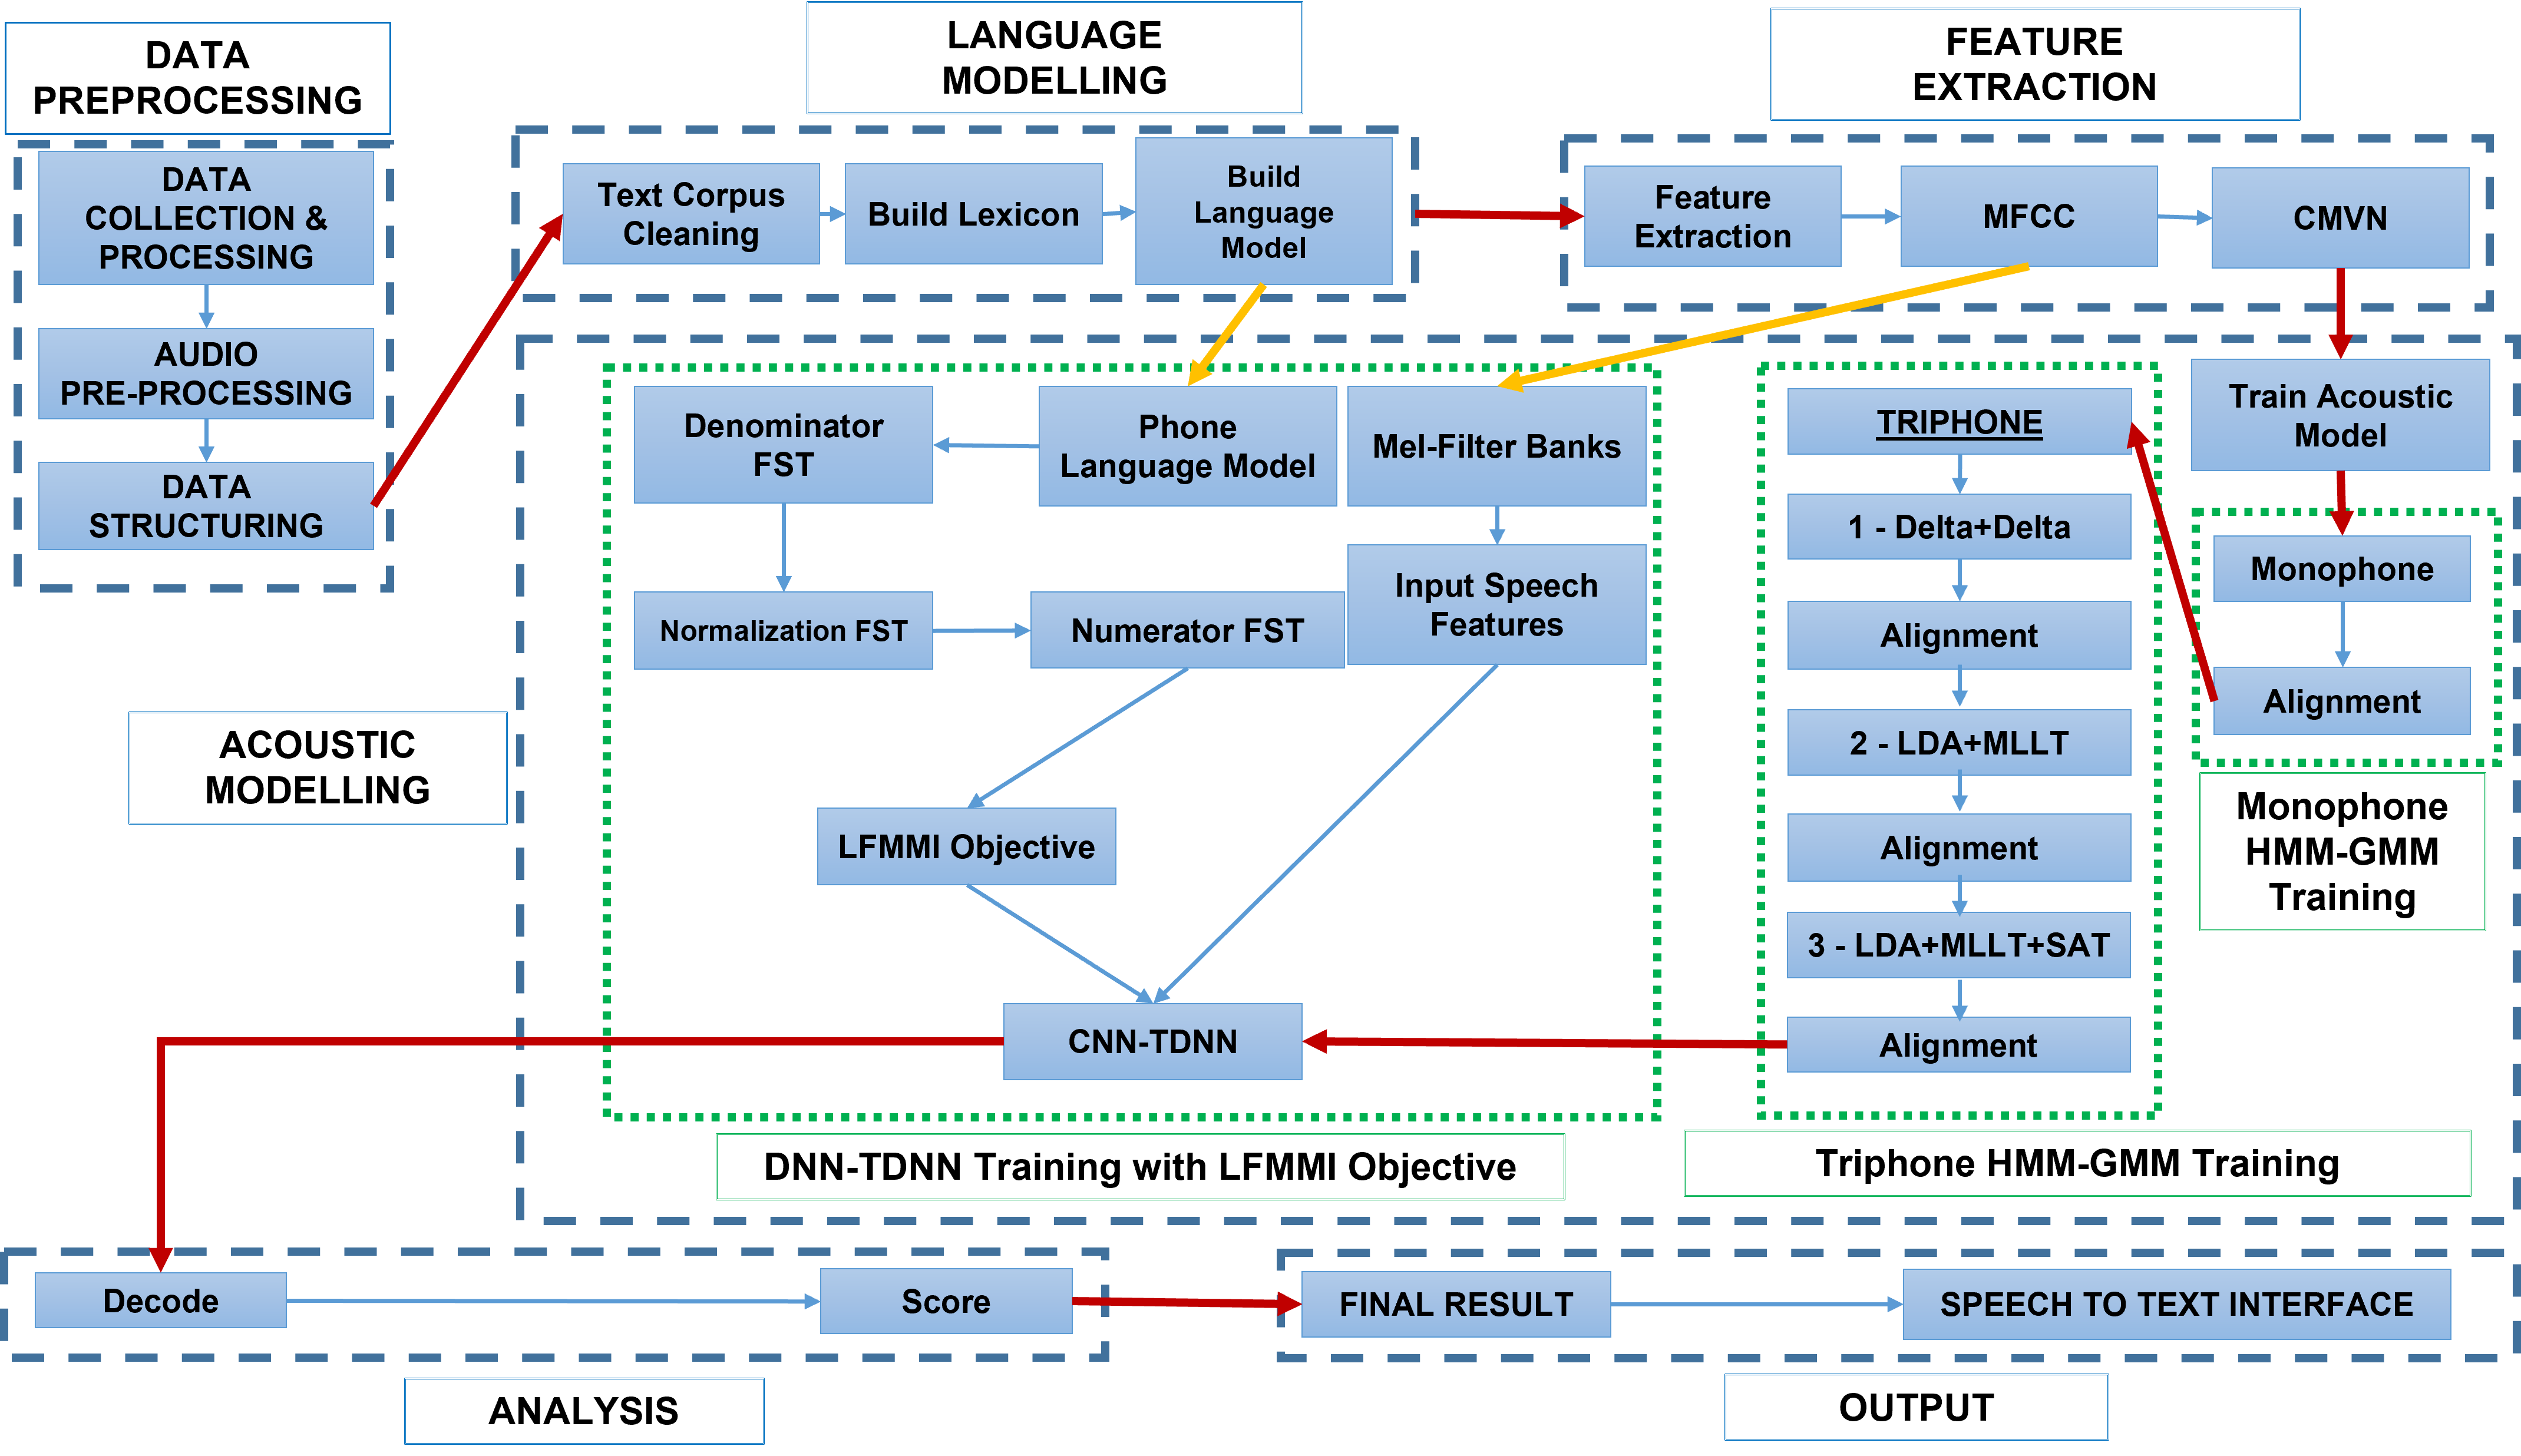
\includegraphics[width=1.5\textwidth]{img/workflow.png}
    \caption{Our Working Pipeline}
    \label{fig:working_pipeline}
\end{figure}
\end{landscape}

\newpage

%Another observation was that when compared to TDNN, CNN-TDNN tends to perform slightly better in less clean data-sets (in this case was called test-other data-set) which drew our attention towards using CNN-TDNN for training acoustic model. Many popular Deep Learning-based End to End ASR engines are available like DeepSpeech 2 \cite{amodei_deep_2015-1} but they need a massive amount of labelled data, which is not available in Urdu. Hence we decided to use CNN-TDNN for training of our Hybrid HMM-DNN ASR. Our long-term approach was to train 10 hours of data to make a strong model and use it to transcribe other audio files to build up our database to 10000 hours and then apply Deep Learning Models on the golden big data-set.

\section{Data Collection and Processing}
\label{sec:Data_preprocessing}

We had huge amount of unlabelled data available. We also had time and budget constrained. There was only one machine available in our Experimental Setup with which we had to build up the ASR. Deep Learning tends to take long time in training which means that errors will be identified after even longer time which makes the process time consuming. 

%\begin{figure}[h]
%    \centering
%    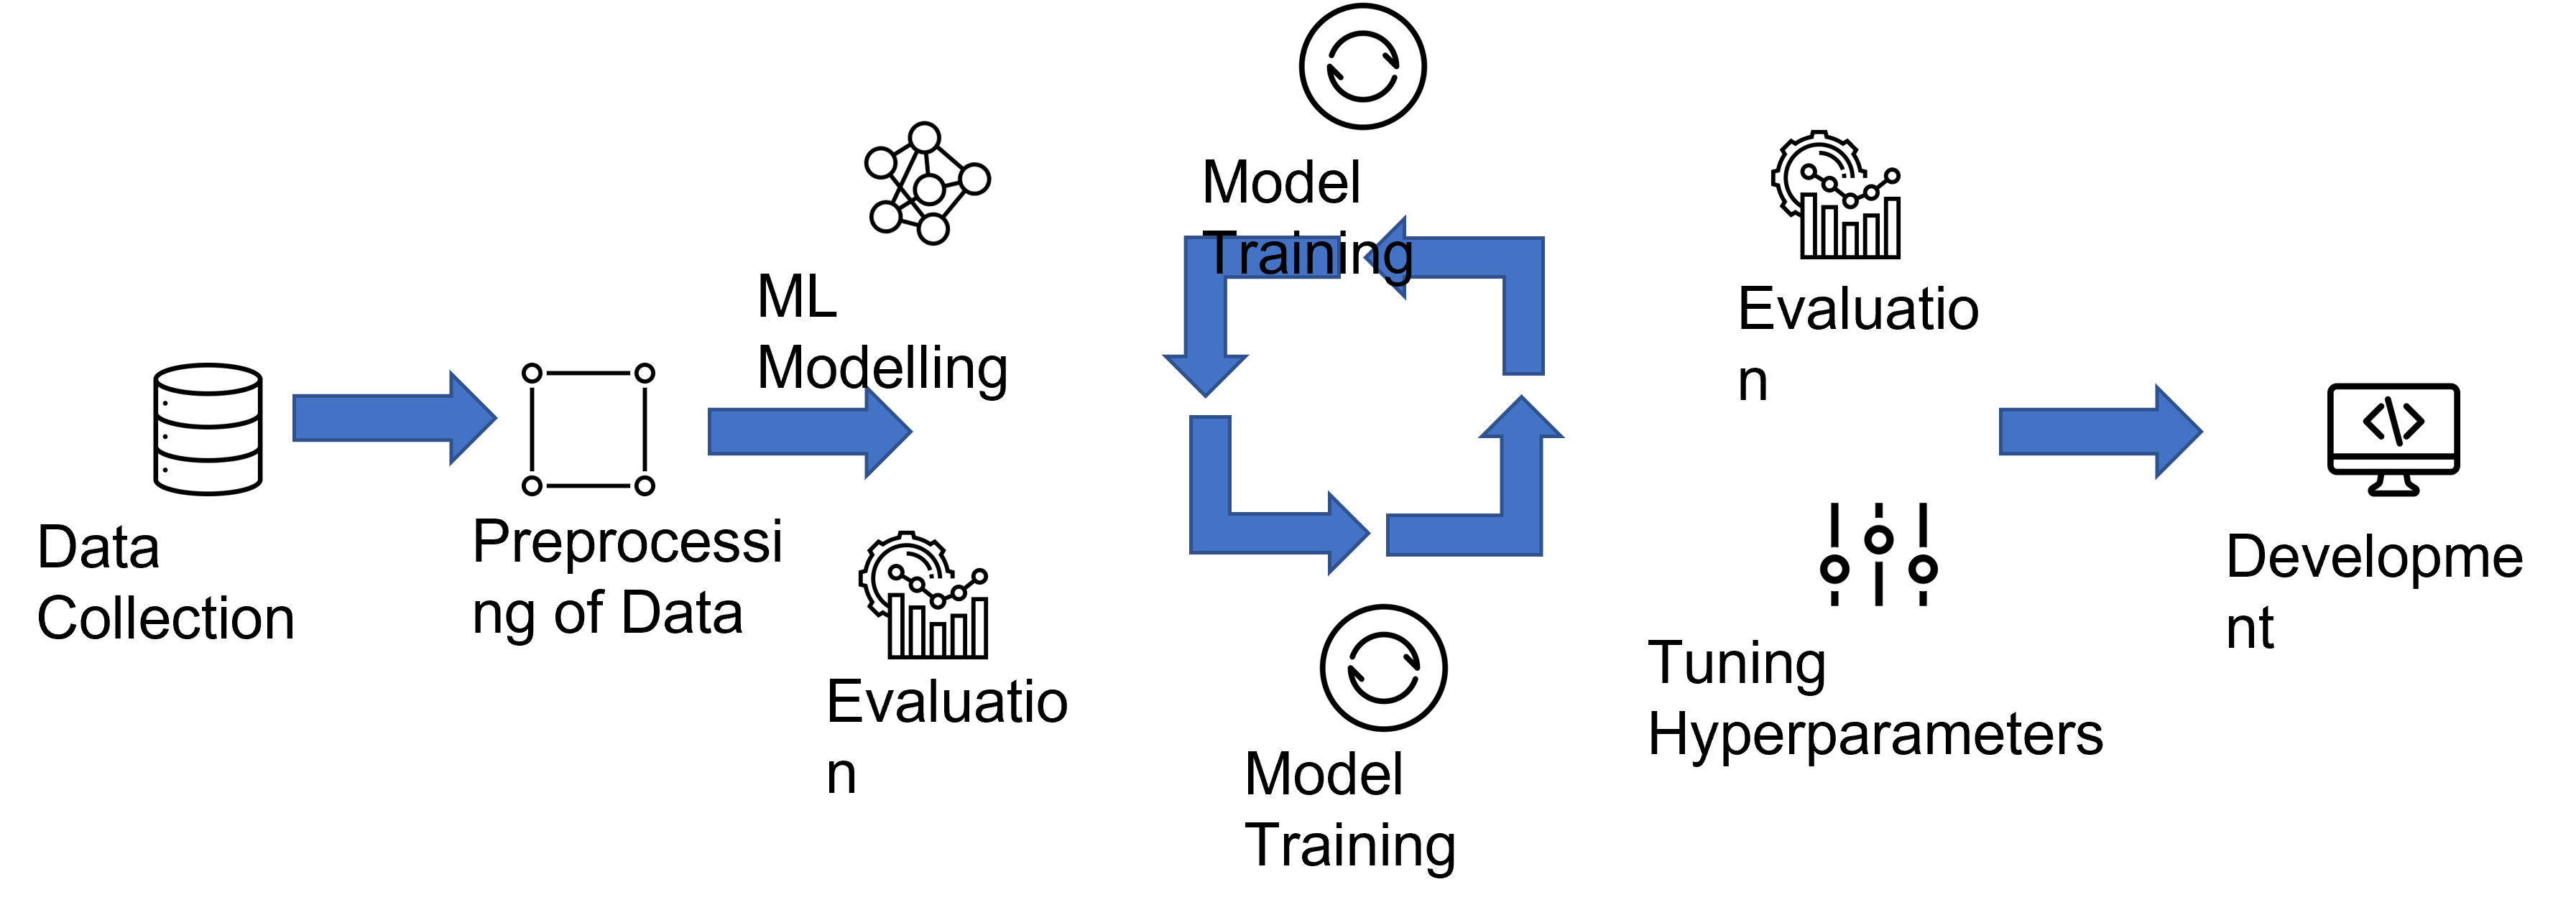
\includegraphics[width=0.9\textwidth]{img/model_centric_ml.png}
%    \caption{Model Centric Machine Learning Approach}
%    \label{fig:modelcentric-ML-approach}
%\end{figure}
%\begin{figure}[h]
%    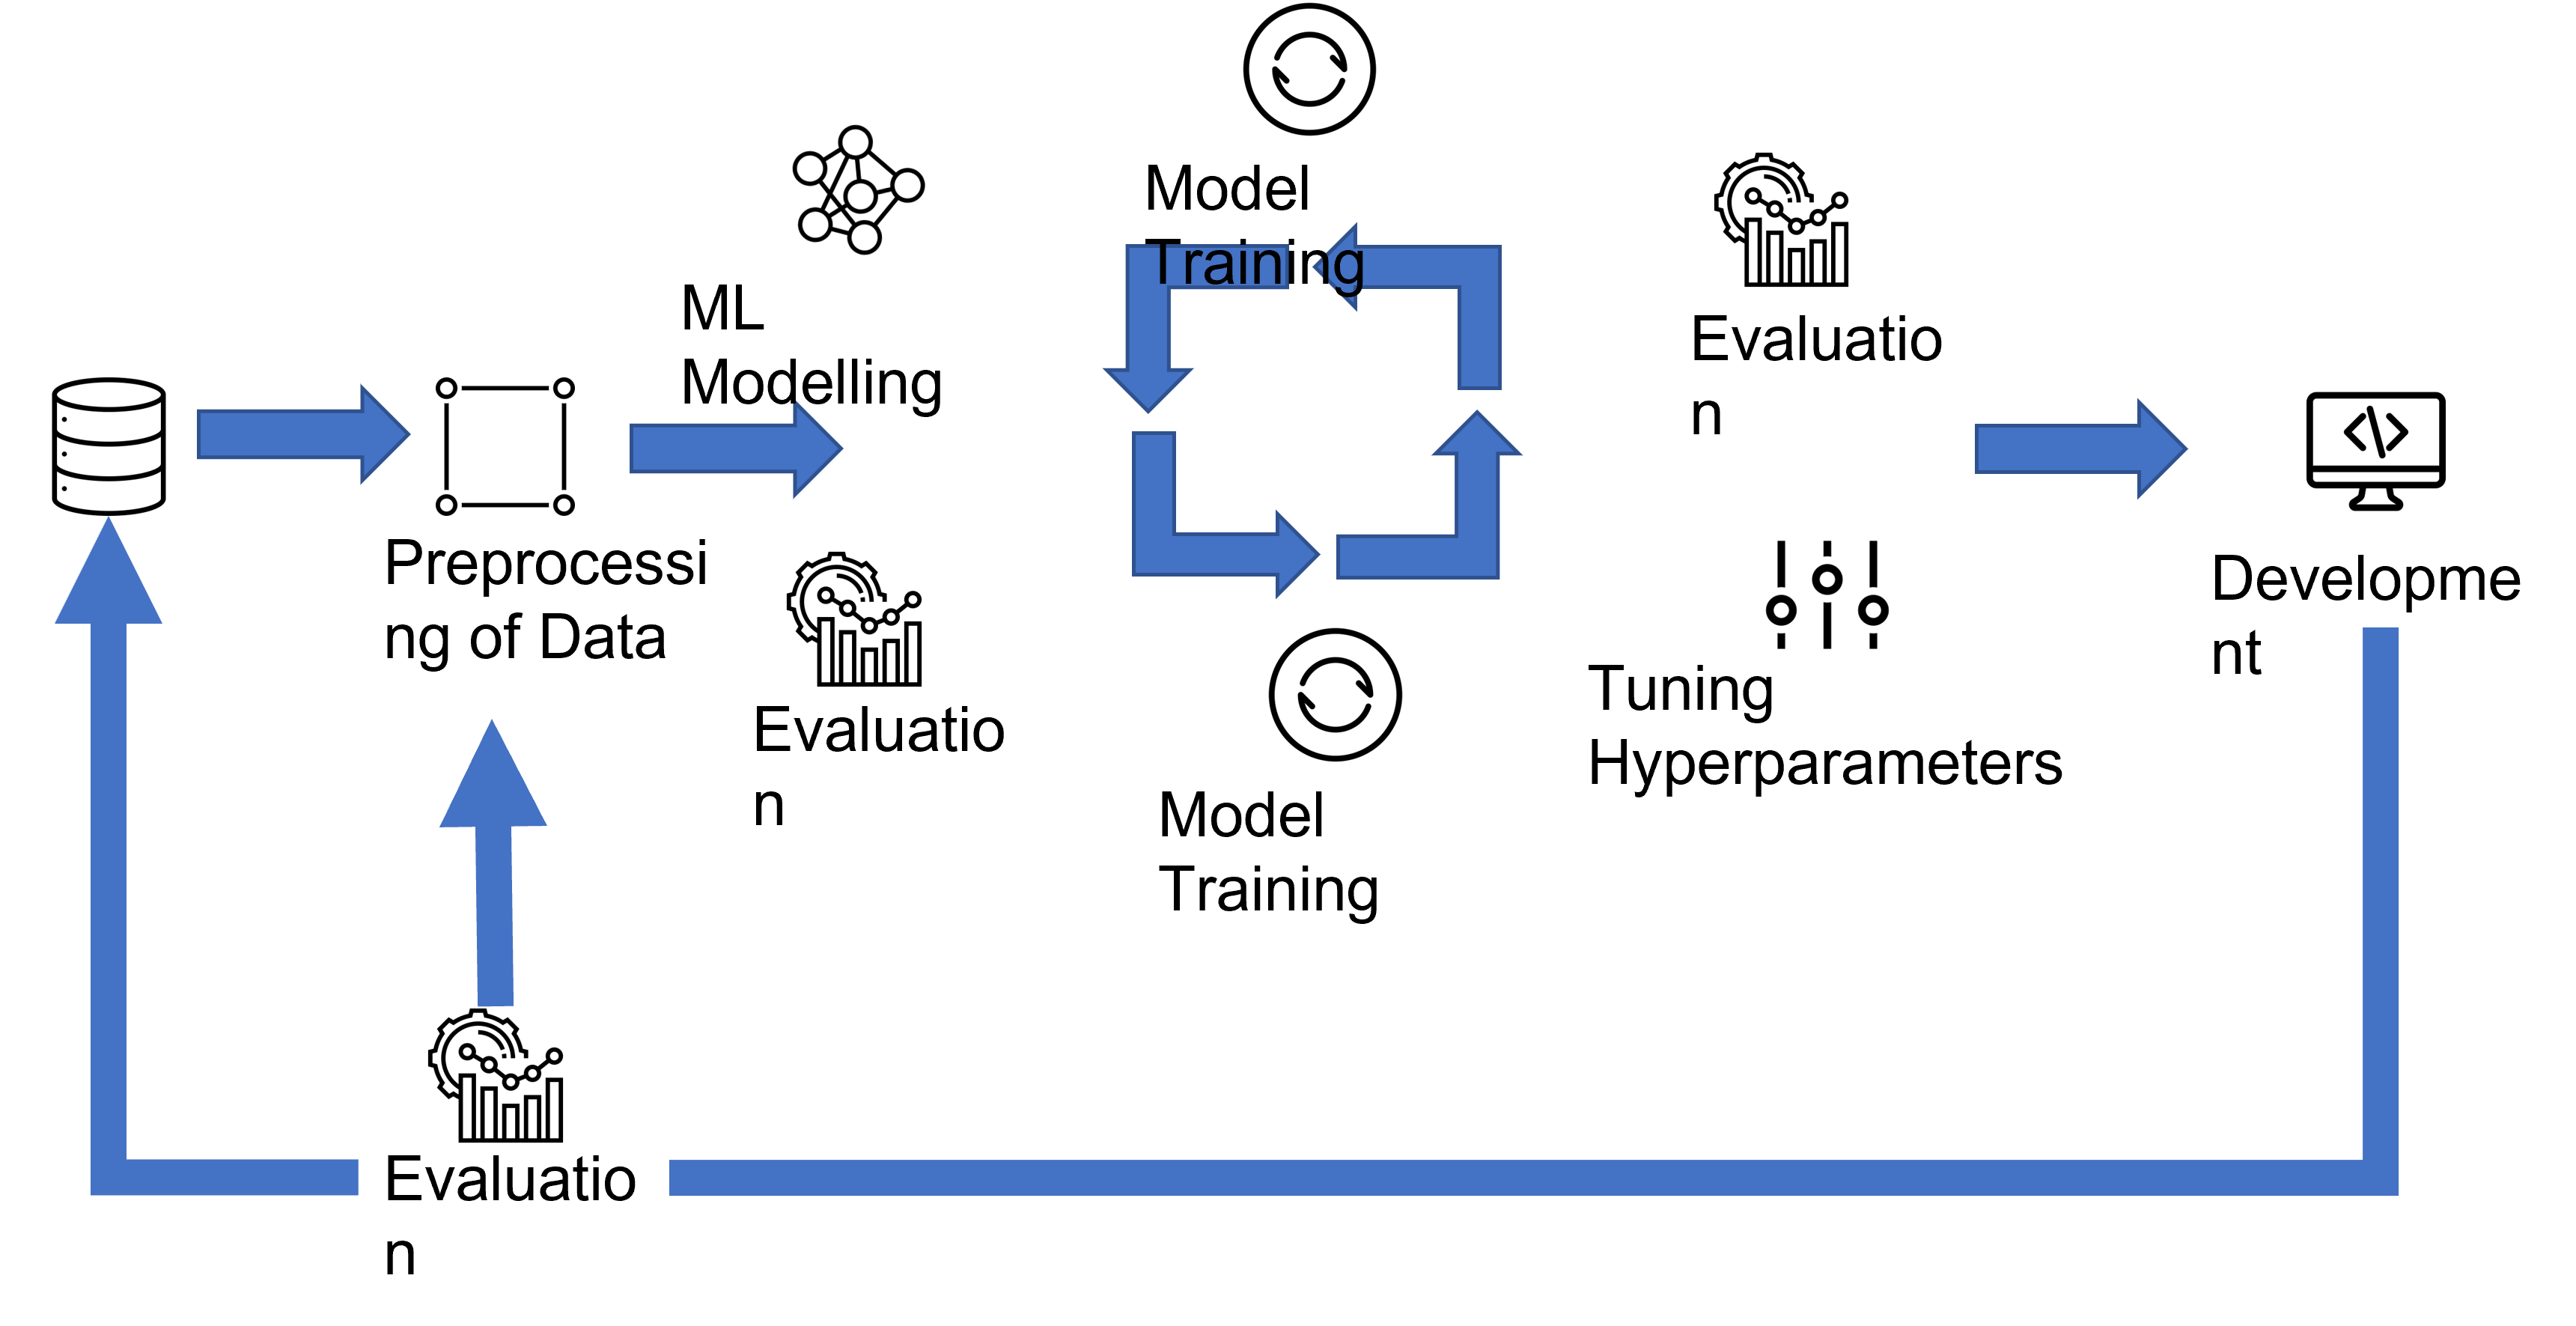
\includegraphics[width=0.9\textwidth]{img/data_centric_ml.png}
%    \caption{Data Centric Machine Learning Approach}
%    \label{fig:datacentric-ML-approach}
%\end{figure}

In this stage we focused on collection and labelling of data. The Data-Centric Approach \cite{patel_data-centric_2021} focuses on reviewing our data iteratively whenever we faced any error in the process, instead of only focusing on tweaking our model. Labelling quality of data primarily determines the overall quality of the machine model. Data is critical in AI research, and developing a strategy that prioritises obtaining high-quality data is crucial. Relevant data is not only rare and noisy, but also extremely expensive to obtain. The idea is that AI should be treated in the same way that the finest materials would be when building a house. They should be evaluated at each level rather than just once.

The common question is how much data is enough to build a quality model? We are often told more data means more accurate model. However, in any given scenario, Quality trumps quantity and same is what we tried to ensure. A data-set with millions of rows with a lot of noisy observations can lead to an obscured learning process, while a smaller data-set with good quality labels tends to give much better results. Eventually we would want a huge dataset that is accurately annotated on which we can make use of End to End ASR training.

\subsection{Data Sources} 
\label{sub:datasources}
We had a mix of structured and unstructured data, with varying duration (1-20 seconds), available from following sources:
\begin{itemize}
    \item D1 - PRUS \cite{zia_pronouncur_2018} 708 sentences data-set taken from \cite{qureshi_urdu_2021}.
    \item D2 - Sehar’s data-sets \cite{sehar_gul_detecting_2020}
    \item D3 - 250 Isolated words data-set \cite{asadullah_automatic_2016} \cite{noauthor_urdu_nodate}. 
    \item D4 - English and Urdu Alphabet spoken audio data which we collected and labelled ourselves.
        \item D5 - Call center unlabelled audio.
\end{itemize}

\subsection{Audio Pre-Processing}

The sampling rates of audio was largely mixed i.e. some had 8KHz and others had 16KHz frequency. We chose a higher sampling rate of 16000 Hz to have more information of speech signal is saved in the noisy or telephonic data. Generally, for ASR training, it is preferred \cite{noauthor_kaldi_nodate} that audio files with mono channel with 8kHz or 16kHz sampling frequency are used \cite{noauthor_why_nodate}. 

We required mono audio in wav format for training \cite{noauthor_kaldi_nodate} \cite{noauthor_why_nodate}. Most of our data was available in mono and for conversion we our customized script using SoX and ffmpeg \cite{noauthor_sox_nodate}.Wav files, unlike mp3, are raw audio and have no compression applied to them which means there is no loss of information in the audio file.

\begin{figure}[htb]
    \centering
    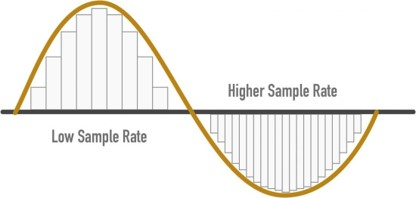
\includegraphics[scale=0.8]{img/samplingrate.jpg}
    \caption{High Sampling Rate vs Low Sampling Rate}
    \label{fig:sampling-rate-high-low}
\end{figure}

Instead of removing noise to maintain speech, we made sure that each utterance had a clean and a noisy counterpart. The ASR would then know for instance how a clean utterance of the word "salaam" sounds like and how "salaam" sounds in noisy environment. Hence we decided to use a higher sampling rate so that more information is retained in the audio. 
%https://en.wikipedia.org/wiki/Sample-rate_conversion

\subsection{Data Structuring}
Our unstructured data-set was the major challenge. We had more than 500 hours of unstructured audios of Call center but we could not spend all the time making We analyzed the scenario of the Call Center and found that the calls were mostly Verification calls which meant primarily we needed good recognition of digits and alphabets in English and Urdu. The normal conversational words were greetings and goodbyes which were standard sentences.

\begin{itemize}
    \item We selected some calls and split them word/sentence/speaker-wise and transcribed them to be included as part of the training set. 5 splits were made speaker wise with utterances for speakers being 348, 8, 7, 55 and 12 clips.
    \item For test 38 utterances were set aside separate to the structured data to judge the results separately. These clips were taken at random, containing out-of-vocabulary words, overlapping speech, distortion and low volume at times, just like in real-life scenario.
    \textit{Note: On average utterances in all cases were 1-20 seconds, covering either single words, multiple words, or up to 3 sentences.} 
\end{itemize}

%For comparison these were also run through google speech recognition API (offline), vocalmatic (online) simonsaysai (online), and dictation.io. The results were 99.9\% error
 
The total audio length for training was 6hours 47minutes and testing was 3h17m. The utterances which sliced from calls were given 0.5-1 second silence in start and end to ensure that there are is no abruptness in the clips, making it easier for ASR to process and align. 

We divided our data into two types; structured and unstructured. Structured data-sets had labeling and transcriptions available whereas the unstructured data-set had no labeling and transcriptions available. 

With regard to the structured data-set the data organization was as follows:
\begin{enumerate}
    \item \textbf{D1:} PRUS \cite{zia_pronouncur_2018} data set (along with Zoraiz Qureshi) 
    \begin{itemize}
        \item Total 7 speakers, 708 sentence-utterances per speaker
        \item Train set = 4 and Test set = 3
    \end{itemize}
    \item \textbf{D2:} Sehar Data-set \cite{sehar_gul_detecting_2020} 
    \begin{itemize}
        \item 100 Sentence-utterances (Malicious), 3 x speakers; 2 x Train and 1 x Test
        \item 86 Sentence-utterances, 7 x speakers; 5 x Train 2 x Test
        \item 5 Word-utterances, 13 x speakers; 10 x Train, 2 x Test
    \end{itemize}
    \item \textbf{D3:} 250-word data set from Asadullah \cite{asadullah_automatic_2016} \cite{noauthor_urdu_nodate} which was also used by Sehar. This had the transcription in Urdu so we had to manually do the transcription in Roman Urdu since that was our chosen mode of writing to avoid spending time building different language models and blending them.    \begin{itemize}
        \item 10 Speakers;
        \item 8 x Train, 2 x Test
    \end{itemize}
    \item \textbf{D4:} English and Urdu Alphabet data which we collected ourselves  
    \begin{itemize}
        \item 11 x Speakers in the Train set. Number of Utterances by each speaker was 28, 102, 206, 60, 28, 26, 37, 135, 256, 185 and 116 clips.
        \item 4 x Speakers in the Test set. Number of Utterances by each speaker was 52, 53, 44 and 55 clips 
    \end{itemize}
    \item \textbf{D5:} Telephonic Data-set samples  
    \begin{itemize}
        \item Training - 5 x speakers and Utterances= 348, 8, 7, 55, 12 clips.
        \item For validation 38 utterances from 2 Speakers
    \end{itemize}
\end{enumerate}

\section{Language Model}
\label{sec:our_lang_modelling}

LM finds the probabilities of words succeeding or preceding a specific word in a given sequence i.e. estimation of likelihood of a word-sequence $W = w_{1},...,w_{n}$ forming a valid sentence, thereby reducing the search radius of the decoders. It can be used to make decisions when the acoustic model output consists of a set of phonemes which can form various alternative sentences. Although these alternatives may be very acoustically similar, the LM selects the one that makes the most sense. LMs are usually formatted in ARPA form which are converted into Finite State Transducers in ASR engines like Kaldi.

\begin{figure}[htb]
    \centering
    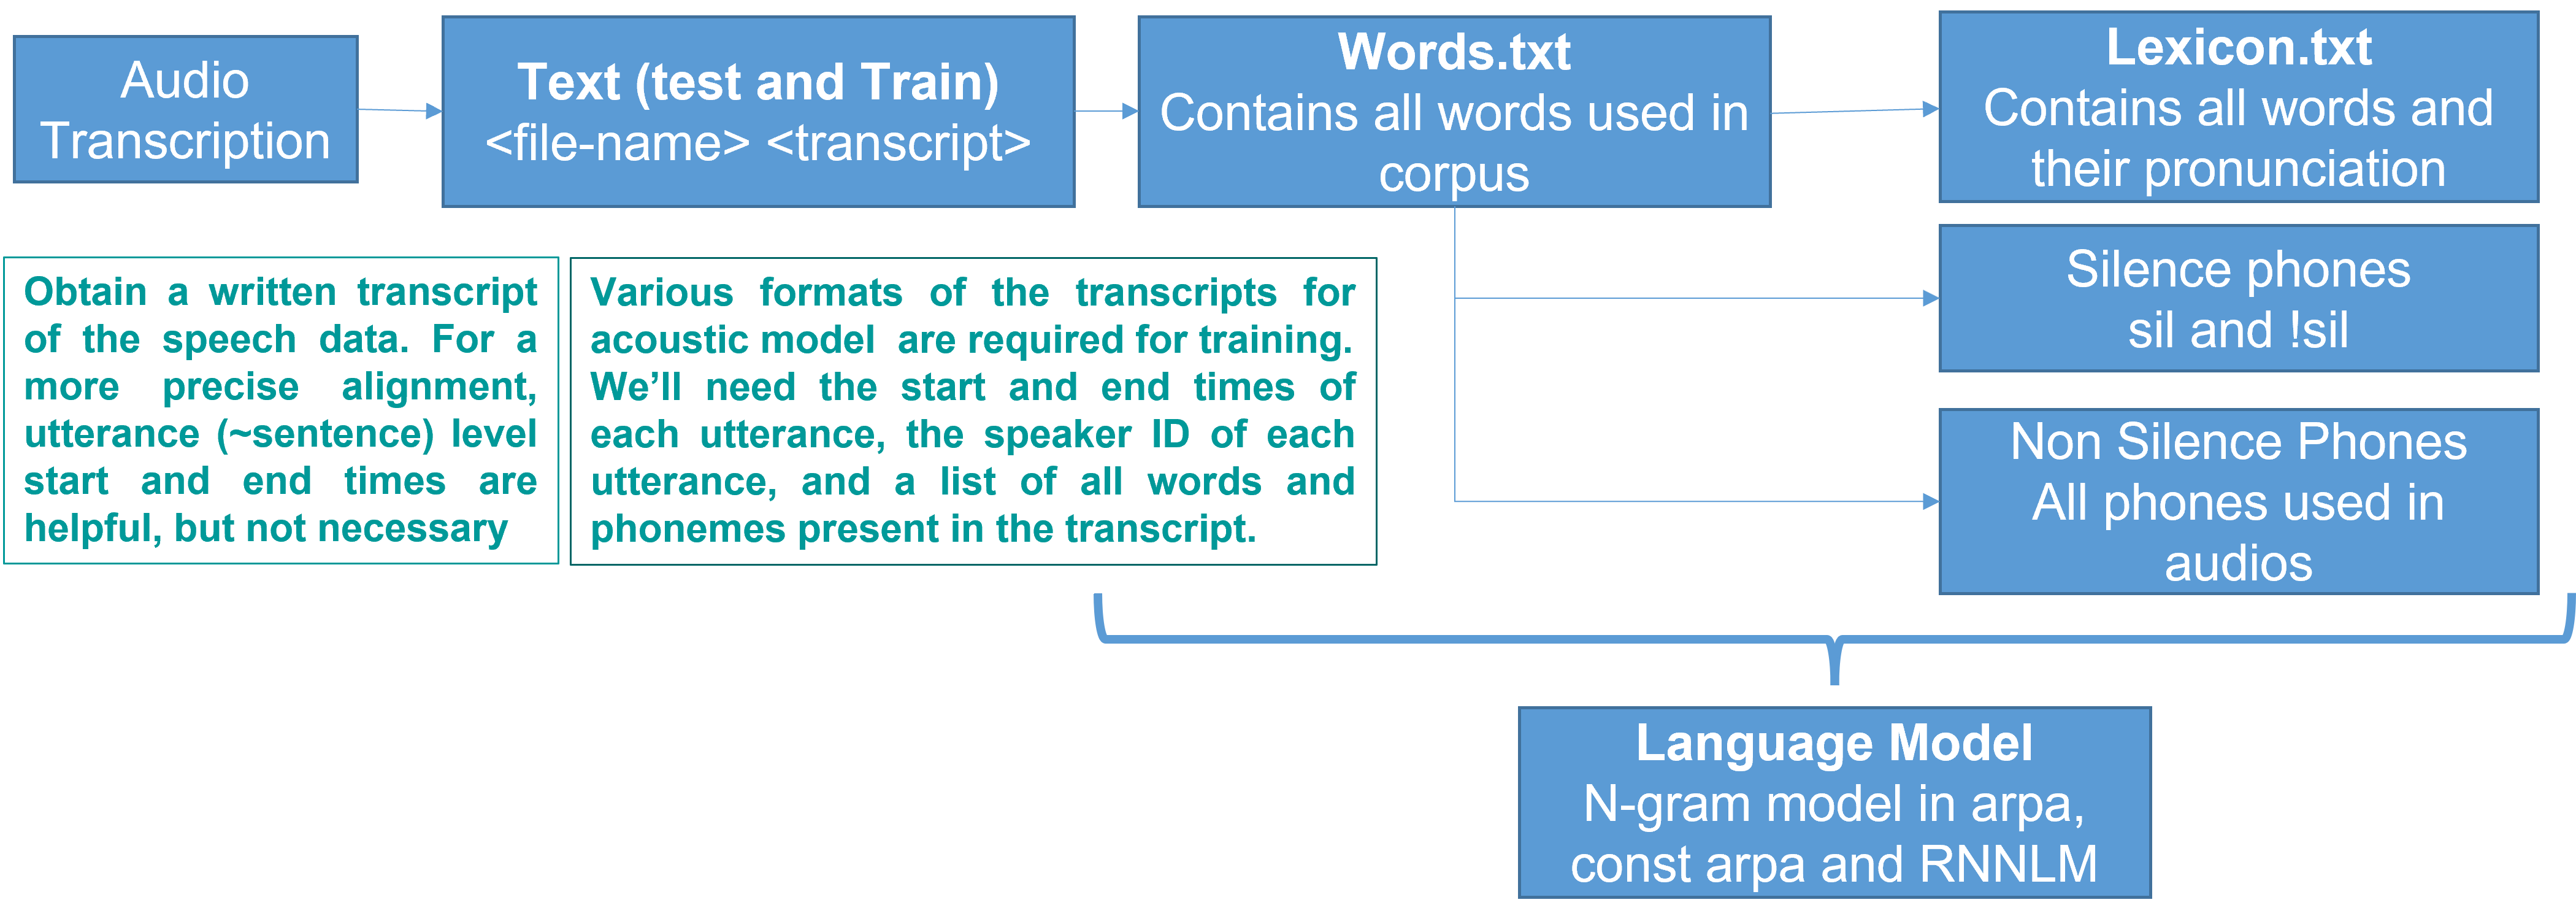
\includegraphics[width=0.95\textwidth]{img/LM.png}
    \caption{Language Model Preparation process}
    \label{fig:lang-model1}
\end{figure}

\subsection{Text Corpus Cleaning}

To prepare LM we combined the transcripts of test and train files in their respective files called \textit{"text"} which contains file-names in one column and their transcripts on the other column. We filtered the corpus and took out all unique words in the text using \textit{cut, sed, uniq and sort} in Linux and saved it as \textit{"words.txt"} \cite{chodroff_corpus_2018}. 

\subsection{Building Lexicon}
There were 7333 words, 137 phones, and 75 non-silence phones in the lexicon, each phoneme represented by a unique combination of symbols and letters. A silence phoneme, 'sil' is added to the 137 phonemes to represent the silence between hyphenated words or the beginning or end of a sentence. The mapping from speaker to utterance was done in spk2utt and utt2spk files.

The English script was used as symbol representations to create a dictionary that shows how words are mapped to phoneme sequences. Word to phoneme dictionary was prepared with help of lextool by CMU \cite{cmu_cmu_nodate} and saved it as \textit{"lexicon.txt"}. Using pronunciation probabilities, multiple pronunciations of the same words were also included.  

\subsection{Building Language Model}

We used SRILM \cite{andreas_stolcke_srilm_2002} for language modelling and building grapheme to phoneme (g2p) sequence-to-sequence model for phonetic mappings of generated lexicon. It was done in local environment to avoid issues with colab \cite{naeem_subspace_2020}. 

There are various types of language modelling based on the number of phonemes considered at once. Assume we have a k-length sequence. Let $P(w_{1}, w_{2}, w_{3},..., w_{k})$ denote the probabilities assigned to the entire sequence by LM. We used a traditional n-gram model using SRILM \cite{andreas_stolcke_srilm_2002}. For an n-gram model, the probability of any word sequence $P(w_{1}, w_{2}, w_{3},..., w_{k})$ is then given as:

\begin{equation}
P(w_{1},w_{2}...,w_{k}) = \prod\nolimits_{i = 1}^{k} a_{i} P(w_{i} | w_{1},...,w_{i-1})
\end{equation}

\section{Feature Extraction and Acoustic Modelling}
\label{sec:feature-extraction-and-AM}
This part computes features from speech wave-form containing elevant information about the linguistic content of the speech while ignoring background noise, emotions etc. The extracted features represent the phones within the words, while other signal-degrading elements such as channel characteristics and background noise are suppressed. MFCC and Perceptual Linear Prediction Coefficients are two popular feature extraction methods (PLP) \cite{backstrom_introduction_2022}. We used the MFCC feature extraction method in our work.  

\begin{figure}[h]
    \centering
    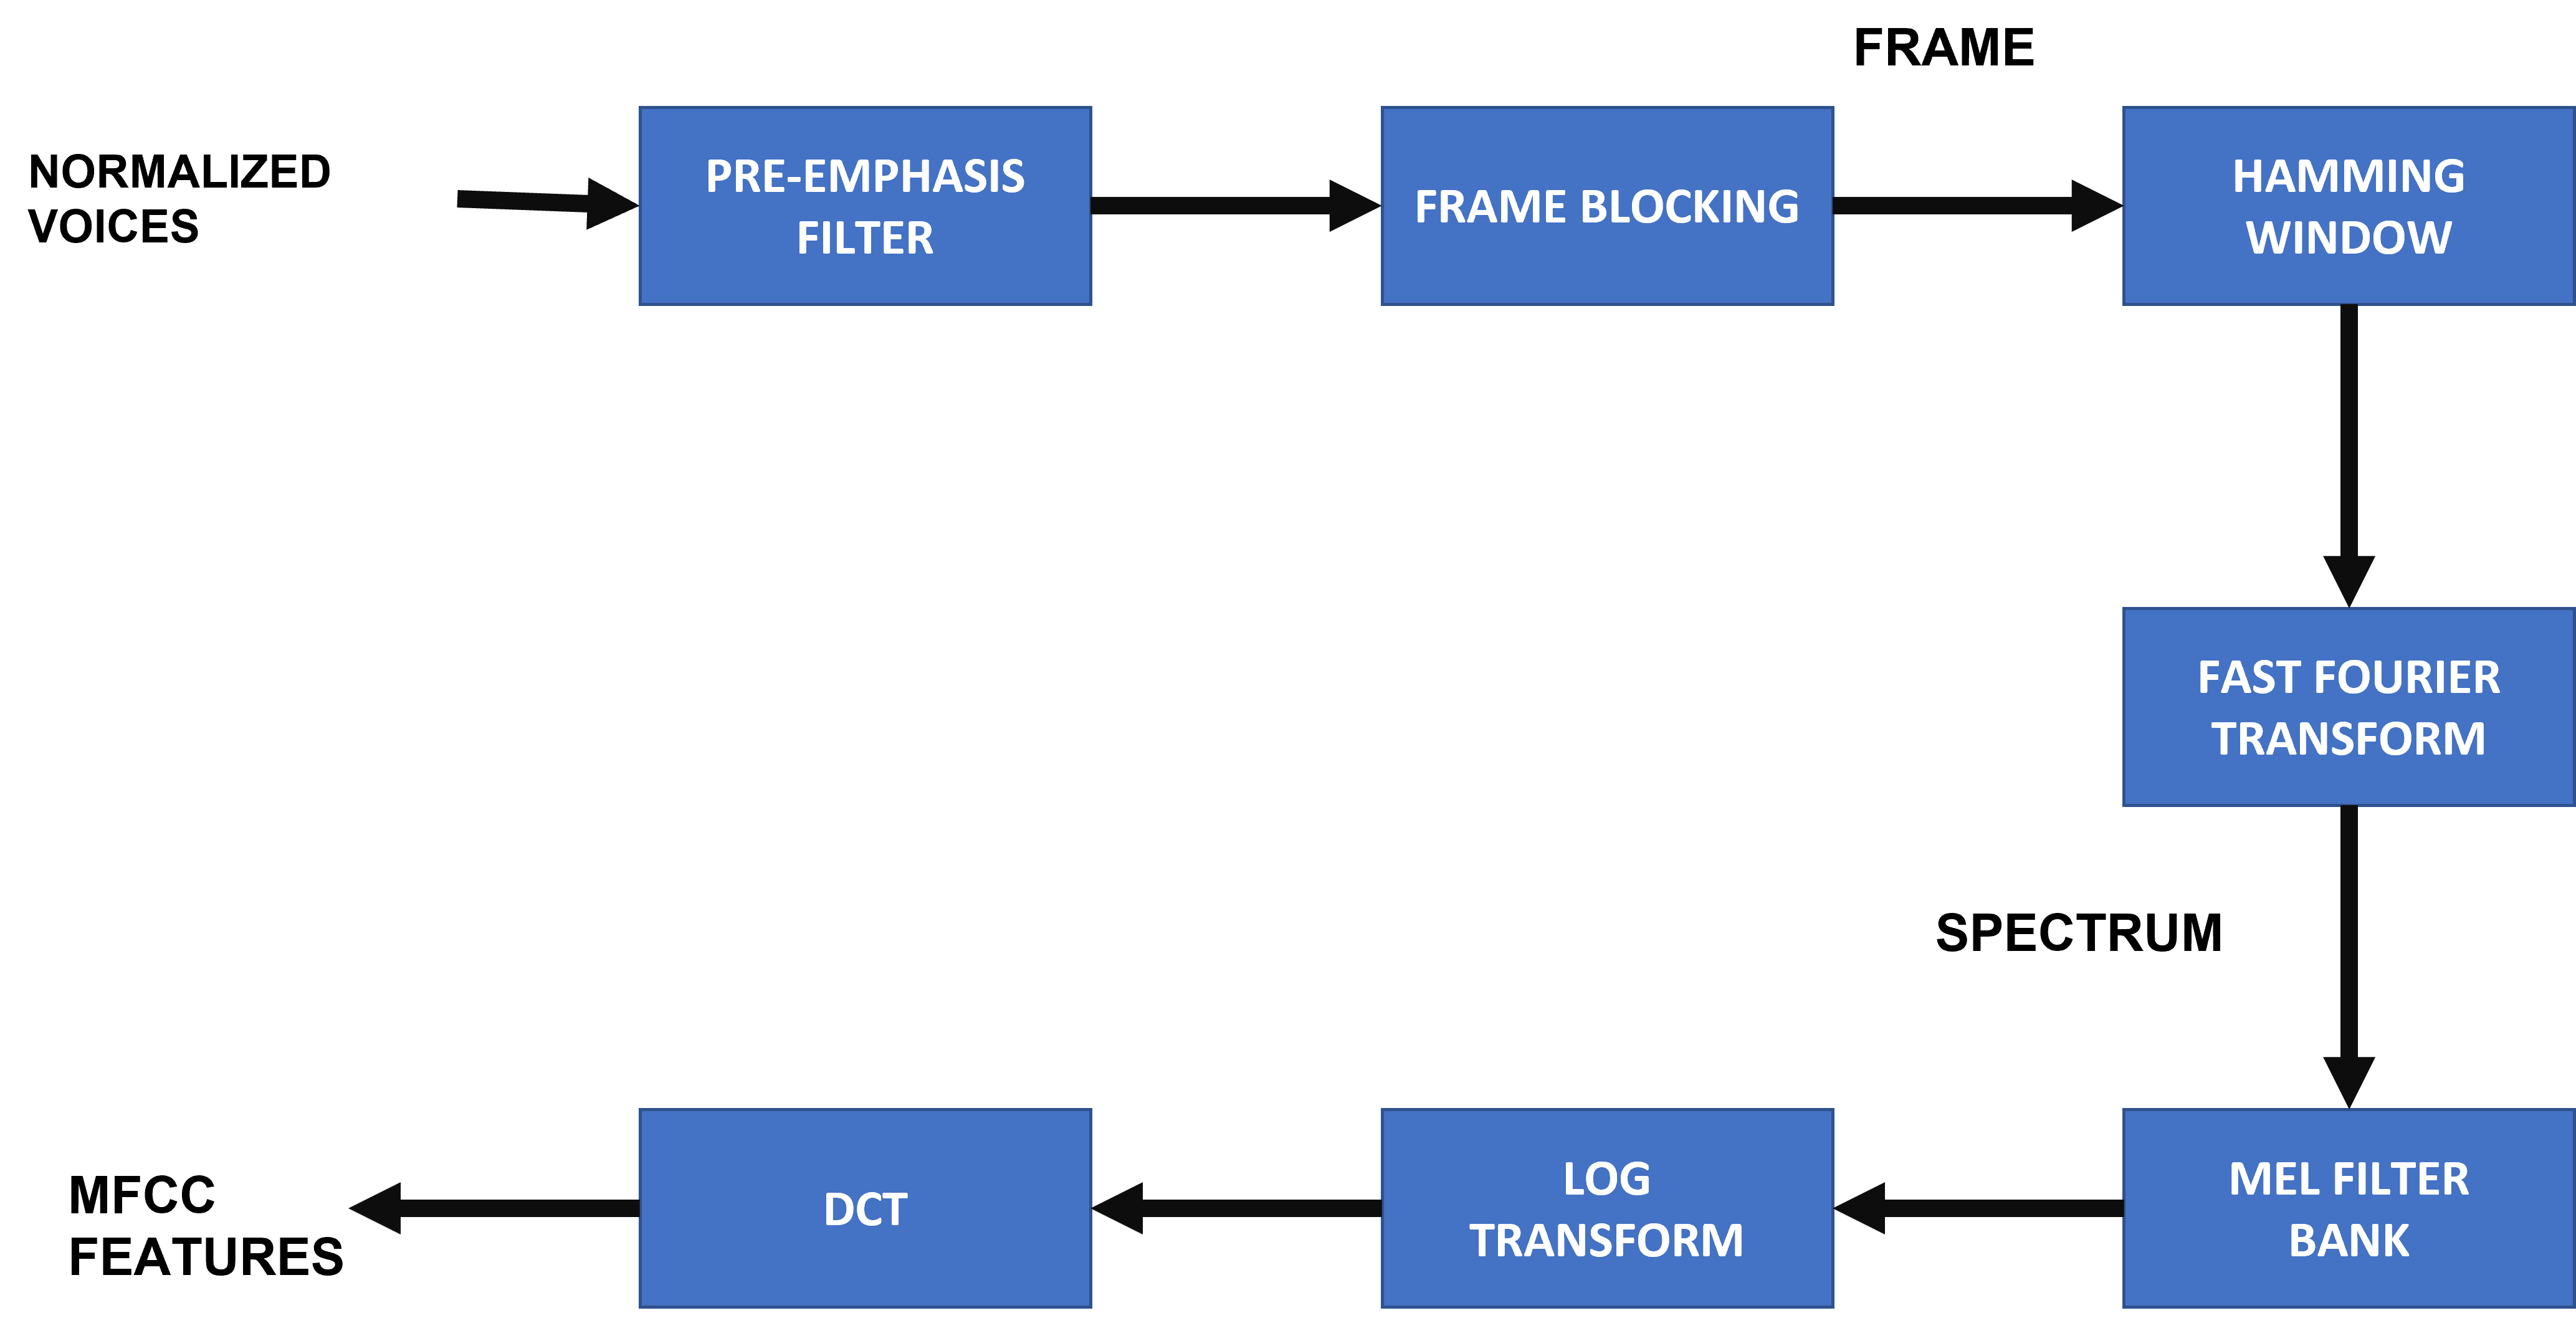
\includegraphics[width=0.8\textwidth]{img/feature extraction.png}
    \caption{Feature Extraction Process}
    \label{fig:Feature-extraction}
\end{figure}

\subsection{MFCC}
\label{sub:MFCC-trg}

The reason MFCC is still extensively used \cite{noauthor_kaldi_nodate} is because they are more easily compressible, being de-correlated; we dump them to disk with compression to 1 byte per coefficient. But we dump all the coefficients, so it’s equivalent to filter-banks times a full-rank matrix without any information loss \cite{raj_note_nodate}. 

MFCCs has a historical momentum and everyone is familiar with it. Hence there is no requirement switch to another model from a familiar one without a very strong reason. If the machine learning algorithm is susceptible to correlated input we use MFCC, a common use case of which are HMM-GMM statistical ASR models. We use Mel-scaled filter banks if the machine learning algorithm is not susceptible to highly correlated input like Neural Networks. 

We extracted 40 MFCCs with  window size of 25ms and 10ms shift, from our training data \cite{naeem_subspace_2020}. The MFCC extraction process begins by conversion of Analogue signals to Digital so that computers can understand them. The next step, Pre-emphasis boosts the energy present in the higher frequencies to counter the spectral tilt issue which is that lower frequencies have more energy. Energy in the higher frequencies are enhanced for easy detection of third formant or F3 i.e. one of the three formants in a phoneme. 

The next step is windowing which is the process of slicing an audio waveform into small overlapping frames because each frame represents a single phoneme which is why we must carefully choose the window length. The entire waveform is divided into 20-40 ms segments. The assumption is that the signal is statistically stationary in this short segment, so features can be assumed to be constant inside this window \cite{raj_note_nodate}. 

Windows overlap as they are 25 ms long and spaced 10 ms apart. In one window, approximately 400 samples are reduced to 13 Cepstral coefficients. The feature is enhanced with additional 13 delta and 13 delta-delta coefficients making a total of 39 Features. Using Hamming Window, this method smooths down the sudden edges in each frame. DFT is then applied to transfer information from the time to the frequency domain. 

After this, a set of triangular band pass filters called Mel filter are applied to the waveform after squaring the DFT output which converts information to the power spectrum. The power spectrum (or estimate of the spectral density of a signal called periodogram) is computed to recognise the frequencies present in this short segment which is accomplished through the use of discrete-time Fourier transforms.  

\subsection{Cepstral Mean and Variance Normalization}
\label{sub:CMVN}
Cepstral calculation as shown in \ref{fig:cepstral} isolates the source from the filter. Pitch information is removed by MFCC features as it is not required in the Speech To Text scenario. The log spectrum contains information about the phone and the pitch. The formants that distinguish phones are identified by the peaks in the spectrum. The IFT can be applied to separate the pitch information from the formants. All that is left to do is take the first 12 independent cepstral values.

\begin{figure}[htb]
    \centering
    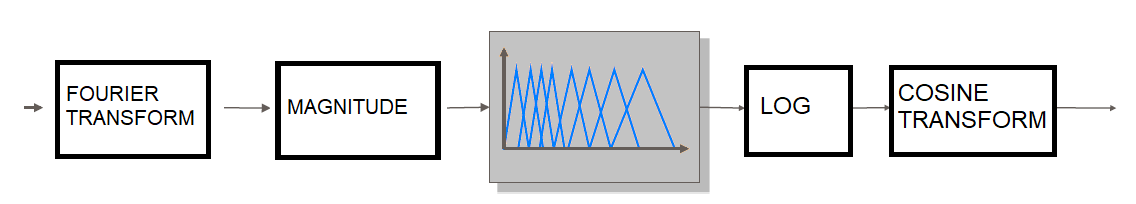
\includegraphics[width=0.8\textwidth]{img/cepstral.png}
    \caption{Cepstral Calculation}
    \label{fig:cepstral}
\end{figure}

Cepstral mean and variance normalisation (CMVN) is a popular noise compensation technique used in a variety of speech applications. It is a computationally efficient noise robust speech recognition normalisation technique. By transforming them to zero mean and unit variance, CMVN eliminates the mismatch between training and test utterances. CMVN performance is known to degrade for short utterances due to a lack of data for parameter estimation and a loss of discriminable information because all utterances are forced to have a zero mean and unit variance.

Cepstral Mean and Variance Normalization techniques (\ref{sub:CMVN}) are most effective for long utterances. Histogram Equalization (HEQ) outperforms CMVN and Cepstral Mean Normalization (CMN) because it matches all moments of the training and test utterances. CMVN matches only the mean and variance while CMN matches only the mean. 

CMVN and HEQ perform worse for short utterances due to a lack of data for parameter estimation. Normalization removes some useful information by forcing all utterances to have the same first and second-order statistics, i.e. zero mean and unit variance \cite{joshi_modified_2016}.

\section{Acoustic Modelling}
\label{sec:training_the_model}

%Kaldi provides various tools to train Acoustic models. We chose to train a Hybrid HMM-DNN model (\ref{sec:hybrid HMM-DNN}) because:
%\begin{itemize}
%    \item We had very limited labeled data. Hence, going completely for Deep %Learning is of no good use.
%    \item Statistical approach may have limitations as discussed earlier but with less data, it works well.
%    \item Our approach was to train 10 hours of data to make a strong model and use it to transcribe other audio files to build up our database and then apply DNN.
%\end{itemize}

In this section we will discuss our Acoustic Model training. Acoustic models are statistical representations of the acoustic information in a phoneme which convert the audio features we created into a sequence of context-dependent phonemes and are required for both automatic speech recognition and forced alignment. 

Various acoustic models such as Mono-phone, Tri-phone, and Chain CNN-TDNN are used to compute the Word Error Rates to validate the ASR system. The dictionary contained 7333 words and 137 phonemes (75 non silence phonemes) based on our training corpus.

Time markings on the phonemes are required for alignment. Hence, the system divides each audio file into equal alignments during alignment, with each division mapped to a different phoneme symbol in the sequence. Each model further refines the alignments using various training techniques before passing them on to the next stage, which is then used for recognition.

We first trained the GMM-HMM model with our training data-set before we can train the DNN-HMM model \cite{li_hybrid_2013}. HMM-DNN acoustic modeling consists of the following steps:
\begin{enumerate}
    \item Mono-phone Training (HMM-GMM).
    \item Tri-phone Training (HMM-GMM) with: 
    \begin{enumerate}[label=\alph*]
        \item Delta features
        \item Delta and delta-delta features
        \item Linear Discriminative Analysis (LDA)
        \item Maximum Likelihood Linear Transform (MLLT)
        \item Speaker adapted training (SAT), i.e. training on feature space maximum likelihood linear regression (fMLLR) adapted features
    \end{enumerate}
    \item HMM-DNN model training using LF-MMI and CNN-TDNN \cite{ghahremani_acoustic_2016}.
\end{enumerate} 

\begin{figure}[h]
    \centering
    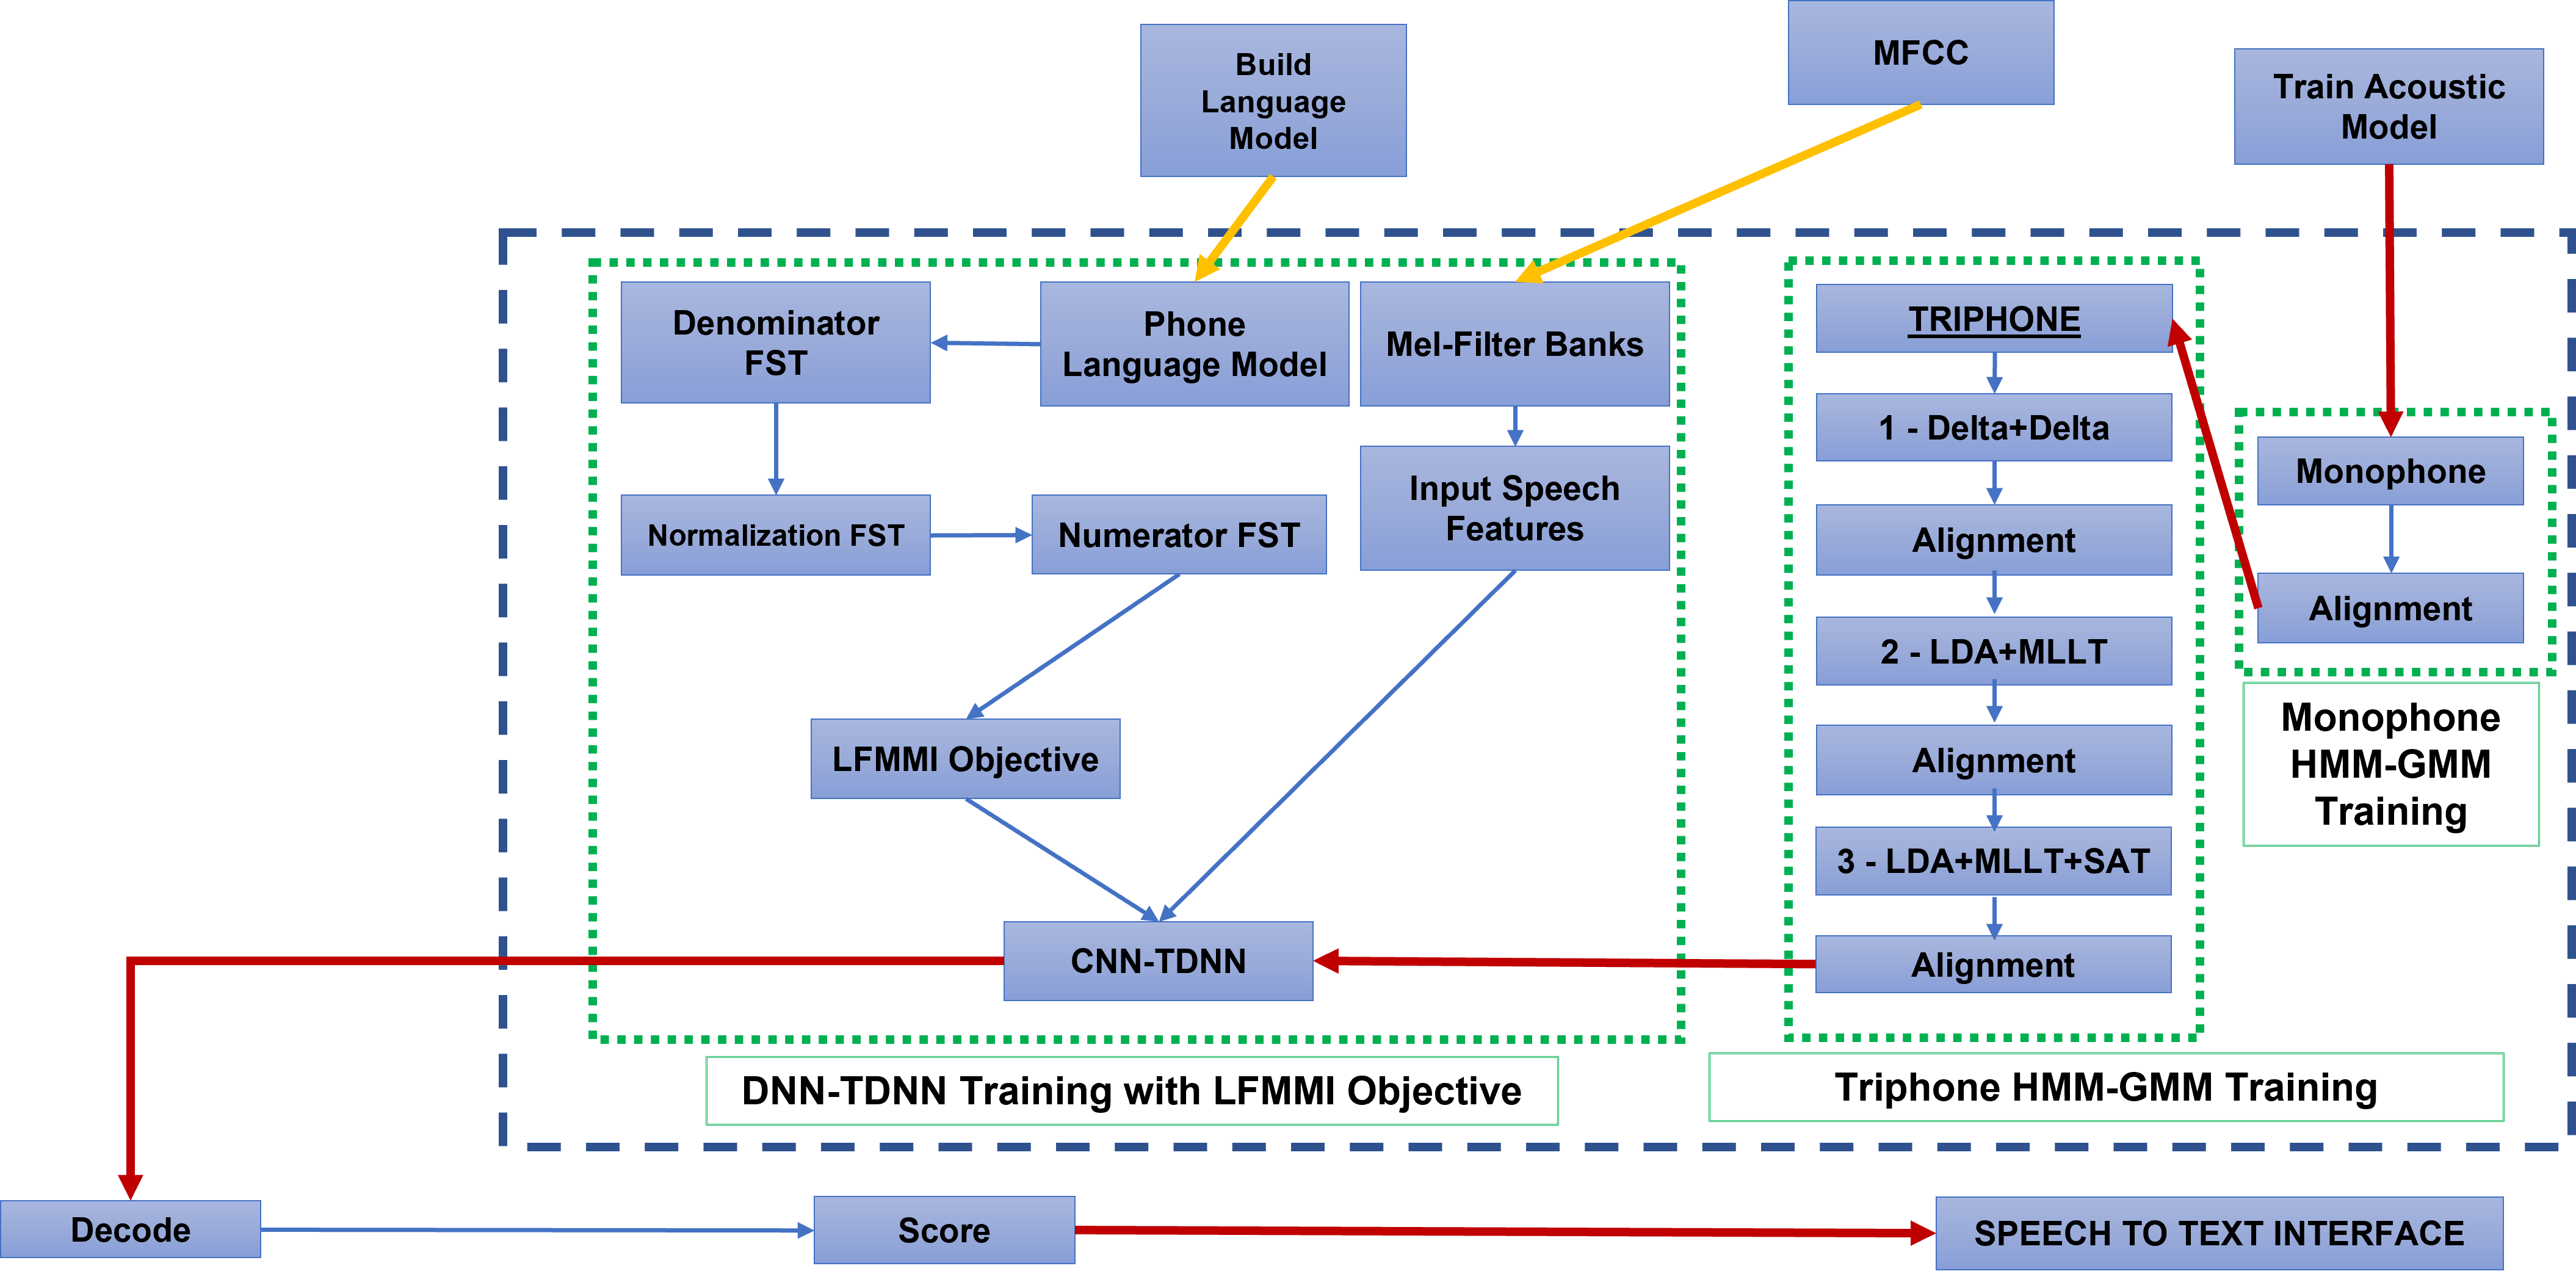
\includegraphics[width=0.95\textwidth]{img/Training-acoustic-model.png}
    \caption{Acoustic Modelling Workflow}
    \label{fig:acoustic-modelling-flow}
\end{figure}

\subsection{Mono-phone Training}
\label{sub:mono-phone}
The first step in training Acoustic Model for HMM-DNN system is to build a simple HMM-GMM acoustic model or mono-phone model in which the HMM states model context-independent phones which is used to force-align the training data-set so that rough estimates of phone boundaries can be obtained for a more complex model. %\cite{patil_automatic_2016} 

Mono-phone model does not include any contextual information about the preceding or the following phone and is used as a building block for the tri-phone models that utilize contextual information. %\cite{benesty_springer_2009}

After mono-phone training, we will align the audio with the acoustic models before moving on to the next training step, tri-phone training. The parameters of the acoustic model are estimated in acoustic training steps; however, the process can be improved by cycling through training and alignment phases, also known as Viterbi training. The Expectation Maximization and Forward-Backward algorithms are related but more computationally expensive procedures.

Additional training algorithms can improve or refine the model's parameters by using the output of aligning the audio to the reference transcript with the most recent acoustic model. As a result, there will be an alignment step after each training step in which the audio and text can be realigned. 

\subsection{Tri-phone Training}
\label{sub:tri-phone}
Phonemes will vary considerably depending on their particular context, while mono phone models represent simply the acoustic parameters of a single phoneme. The tri-phone models represent a phoneme variant within the context of two other phonemes (left and right). %\cite{benesty_springer_2009}

The data-set does not contain (and will never contain) all tri-phone units. There are three phonemes and thus three tri-phone models, but only a subset of those will appear in the data. To gather enough statistics for the data, the unit must appear multiple times in the data. A phonetic decision tree divides these tri-phones into fewer acoustically distinct units, reducing the number of parameters and making the problem computationally feasible.

In contrast to the mono-phone model, which compares each phoneme individually and assigns weights based on the probability of match, the acoustic parameters in tri-phone models are represented for a block of three consecutive phonemes. We can assign one HMM state from a total of 49 x 3 = 147  for each tri-phone. The training data-set, however, may not contain all of the tri-phones. A decision tree is used to group the tri-phones into a smaller set of distinct units.
%https://jonathan-hui.medium.com/speech-recognition-kaldi-35fec0320496

\begin{figure}[h]
    \centering
    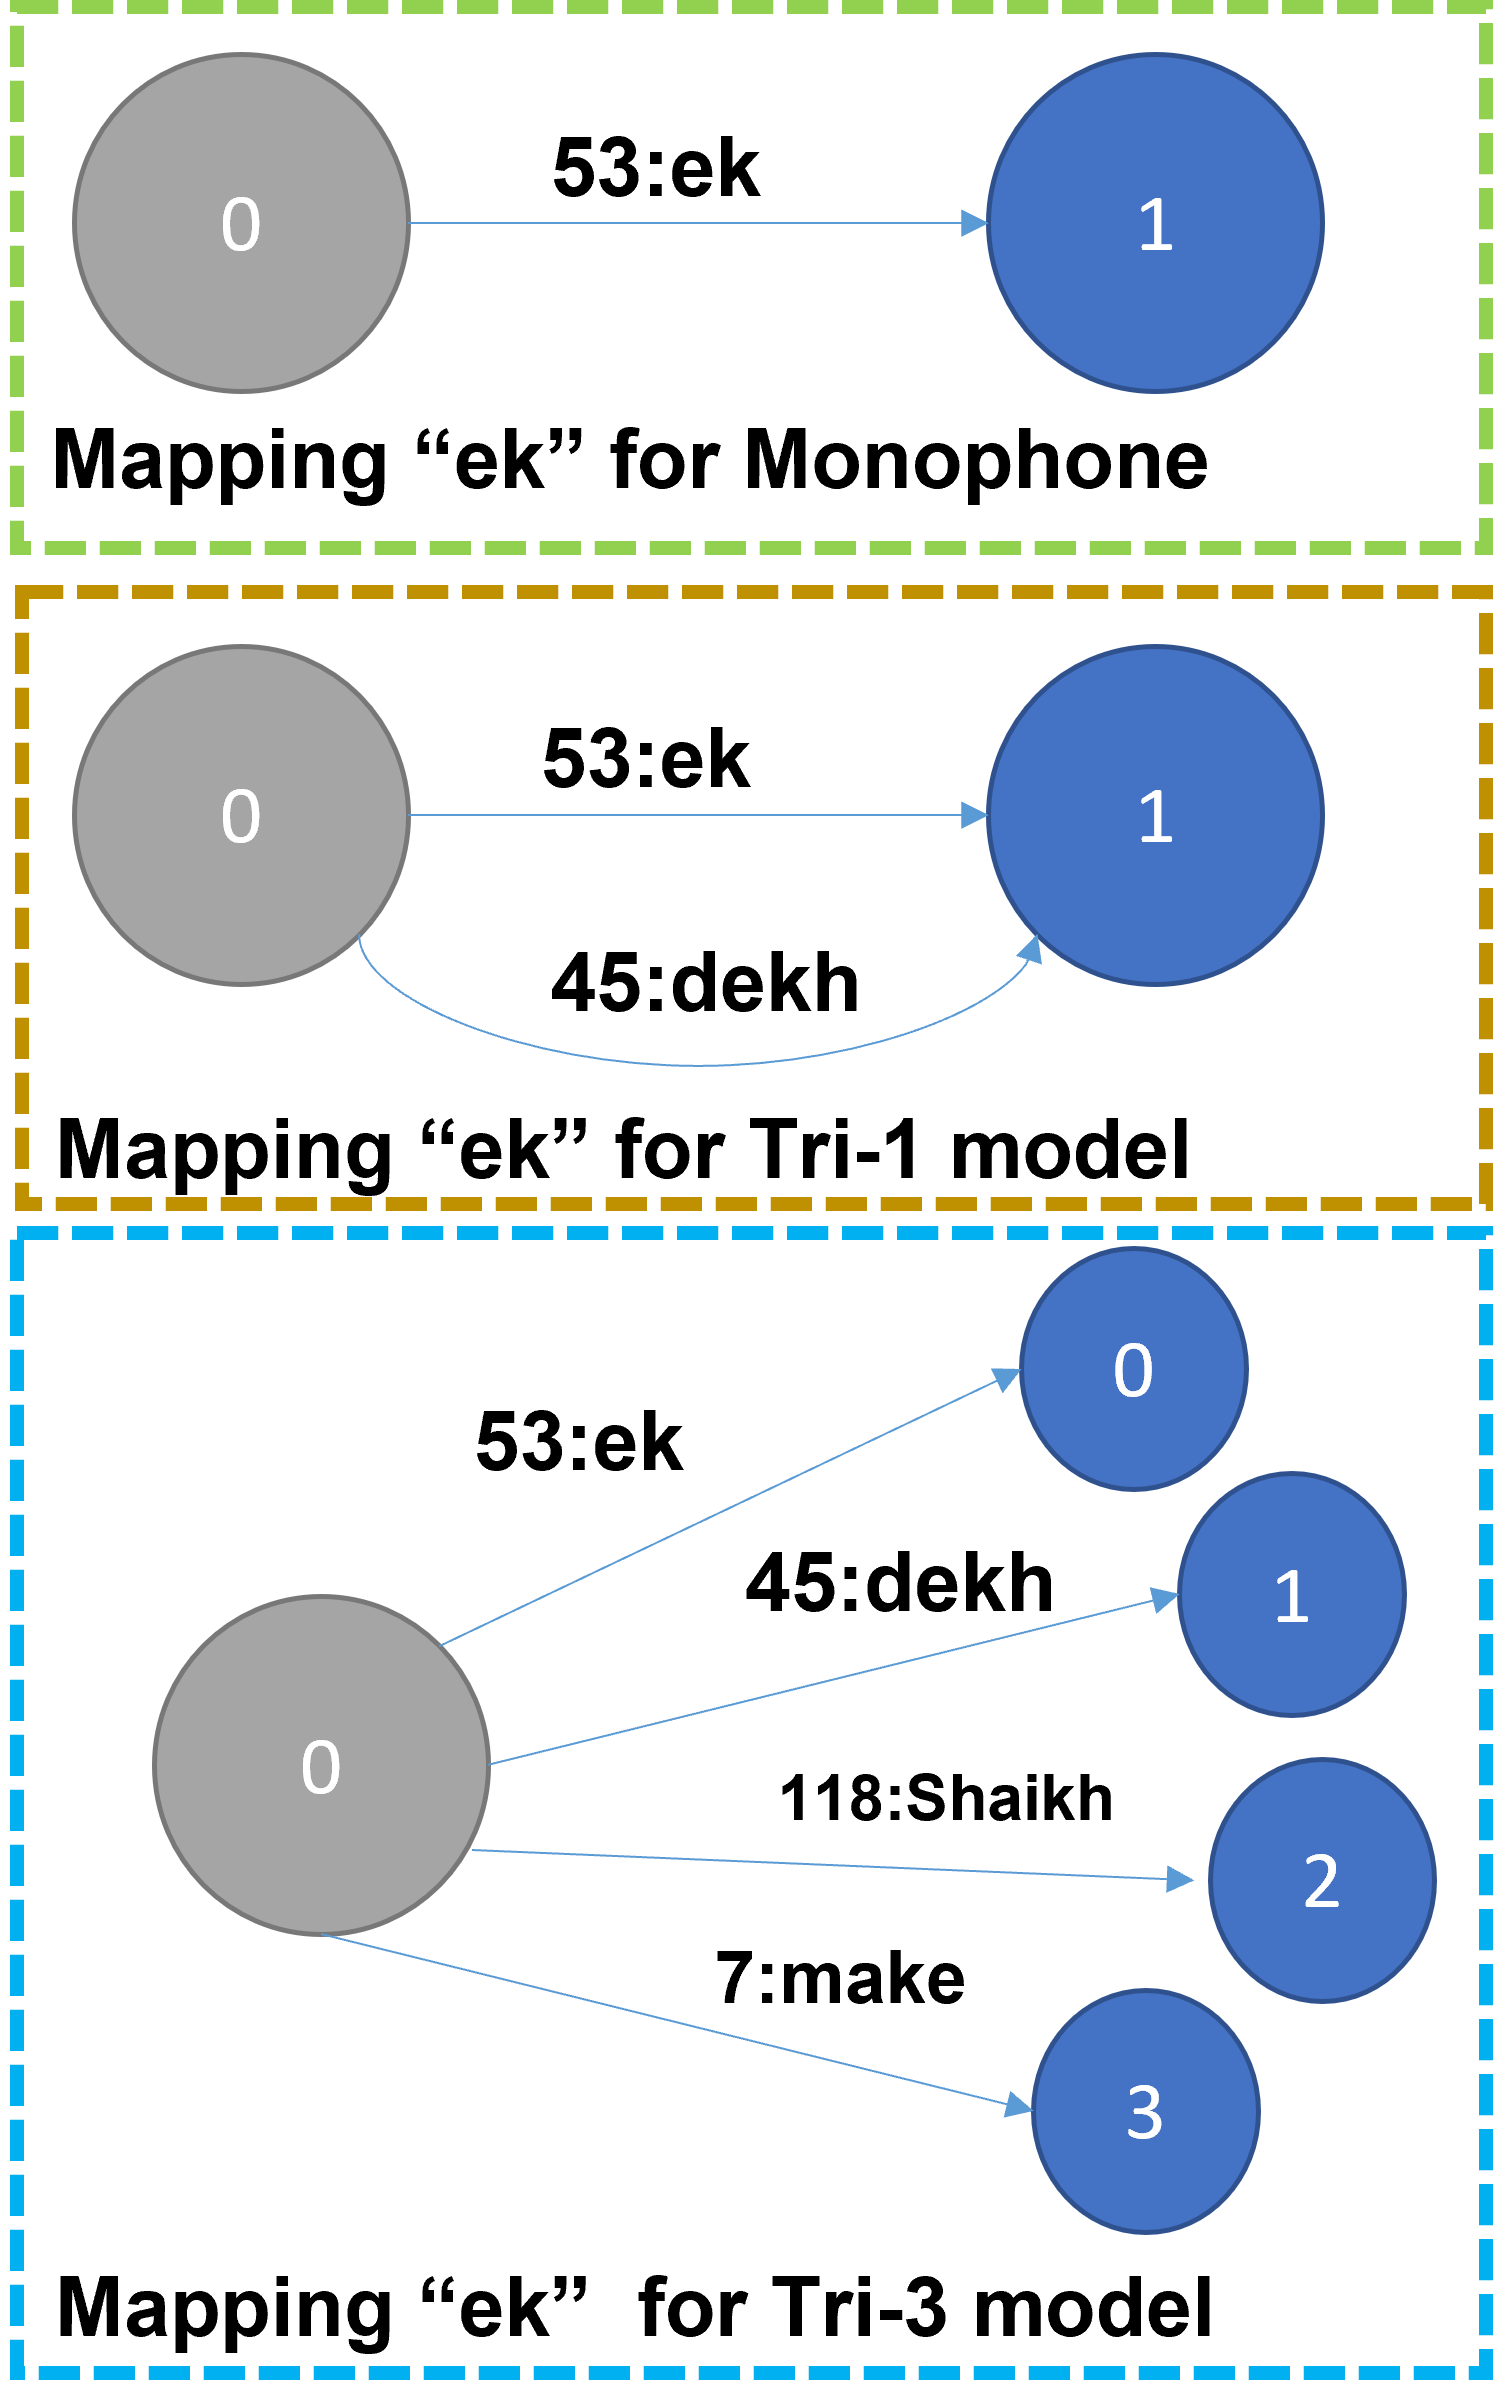
\includegraphics[width=0.4\textwidth]{img/mapping.png}
    \caption{Mapping the word 'ek' in mono-phone and tri-phone}
    \label{fig:mapping-mono-tri}
\end{figure}

The tri-phone model comprises of three types training models which we trained \cite{raj_note_nodate}:
\begin{enumerate}
    \item \textit{Delta and delta-delta training} - This training method computes delta and double-delta features, also known as 'dynamic coefficients,' in conjunction to MFCC features. They are the signal's first and second order derivatives (features). These characteristics are then used for recognition.
    \begin{itemize}
        \item In order to recognize speech better, dynamics of the power spectrum need to be understood i.e. the trajectories of MFCCs over time for which we use delta or differential and delta-delta or acceleration coefficients. 
        \item The delta coefficients are calculated using the following formula:
        \begin{equation}
        d_{t}=\frac{\sum_{n=1}^{N} n(c_{t+n}-c_{t-n})}{2 \sum_{n=1}^{N}n^2}    
        \end{equation}
        The delta coefficient from frame \textit{t} is represented by $d_{t}$ and is computed in terms of $c_{t-n}$ i.e. static coefficients to $c_{t+n}$. We usually take $n = 2$. Acceleration coefficients are similarly computed using differential instead of the static coefficients.
    \end{itemize}
    \item \textit{LDA-MLLT} - The most current TDNN-based architecture uses an \textit{"LDA-like transformation"} that is essentially an \textit{"affine transformation"} of the spliced input. LDA shrinks the feature space by generating HMM states for the feature vectors and the reduced feature space is used to create a transform that is unique to each speaker which is why MLLT is able to incorporate speaker independence.             
    \item \textit{Speaker Adaptive Training (LDA+MLLT+SAT)} - For each speaker, noise and speaker normalisation is performed using a data transform which enables the model to compute the variance due to the phoneme rather than the background environment using its parameters. 
    \begin{itemize}
        \item SAT also performs speaker and noise normalisation by adapting a particular data transform to each individual speaker. 
        \item The data, thus, becomes more homogeneous or standardised, allowing the model to focus its parameters on estimating variance due to the phoneme rather than the speaker or recording environment. Hence, this result has the lowest word error rate. 
        \item Following SAT training, the acoustic model is trained on speaker-normalized features rather than the original features. 
    \end{itemize}

\end{enumerate}

Audio is re-aligned with the acoustic models at the end of each tri-phone training before proceeding on to the next tri-phone model training step. In this step, the alignment algorithms include speaker-independent alignments and FMLLR. The Acoustic Model is no longer trained with the new normalised features after achieving the speaker-normalized features for SAT training. These partially speaker-independent models are used in the alignment process. Various scripts accept various types of acoustic model input but the actual alignment algorithm will always be the same. In the alignment process, speaker-independent alignment will exclude speaker-specific information. This training resulted in 13\% WER and 31.2\% SER.

\section{Neural Network Training with LFMMI Objective \\ Function}
\label{sec:LFMMI-chain}
The DNN model, which introduces the concept of unsupervised training or adaptation, eliminates the need to provide adaptation data in advance. Hence we will enhance our system by modelling the acoustic units with DNN rather than using GMMs. For Neural Network Training, we used Chain CNN-TDNN with LF-MMI as the objective function. The Chain model is outlined in Figure \ref{fig:Chain-Training-outline}.

\begin{figure}[h]
    \centering
    %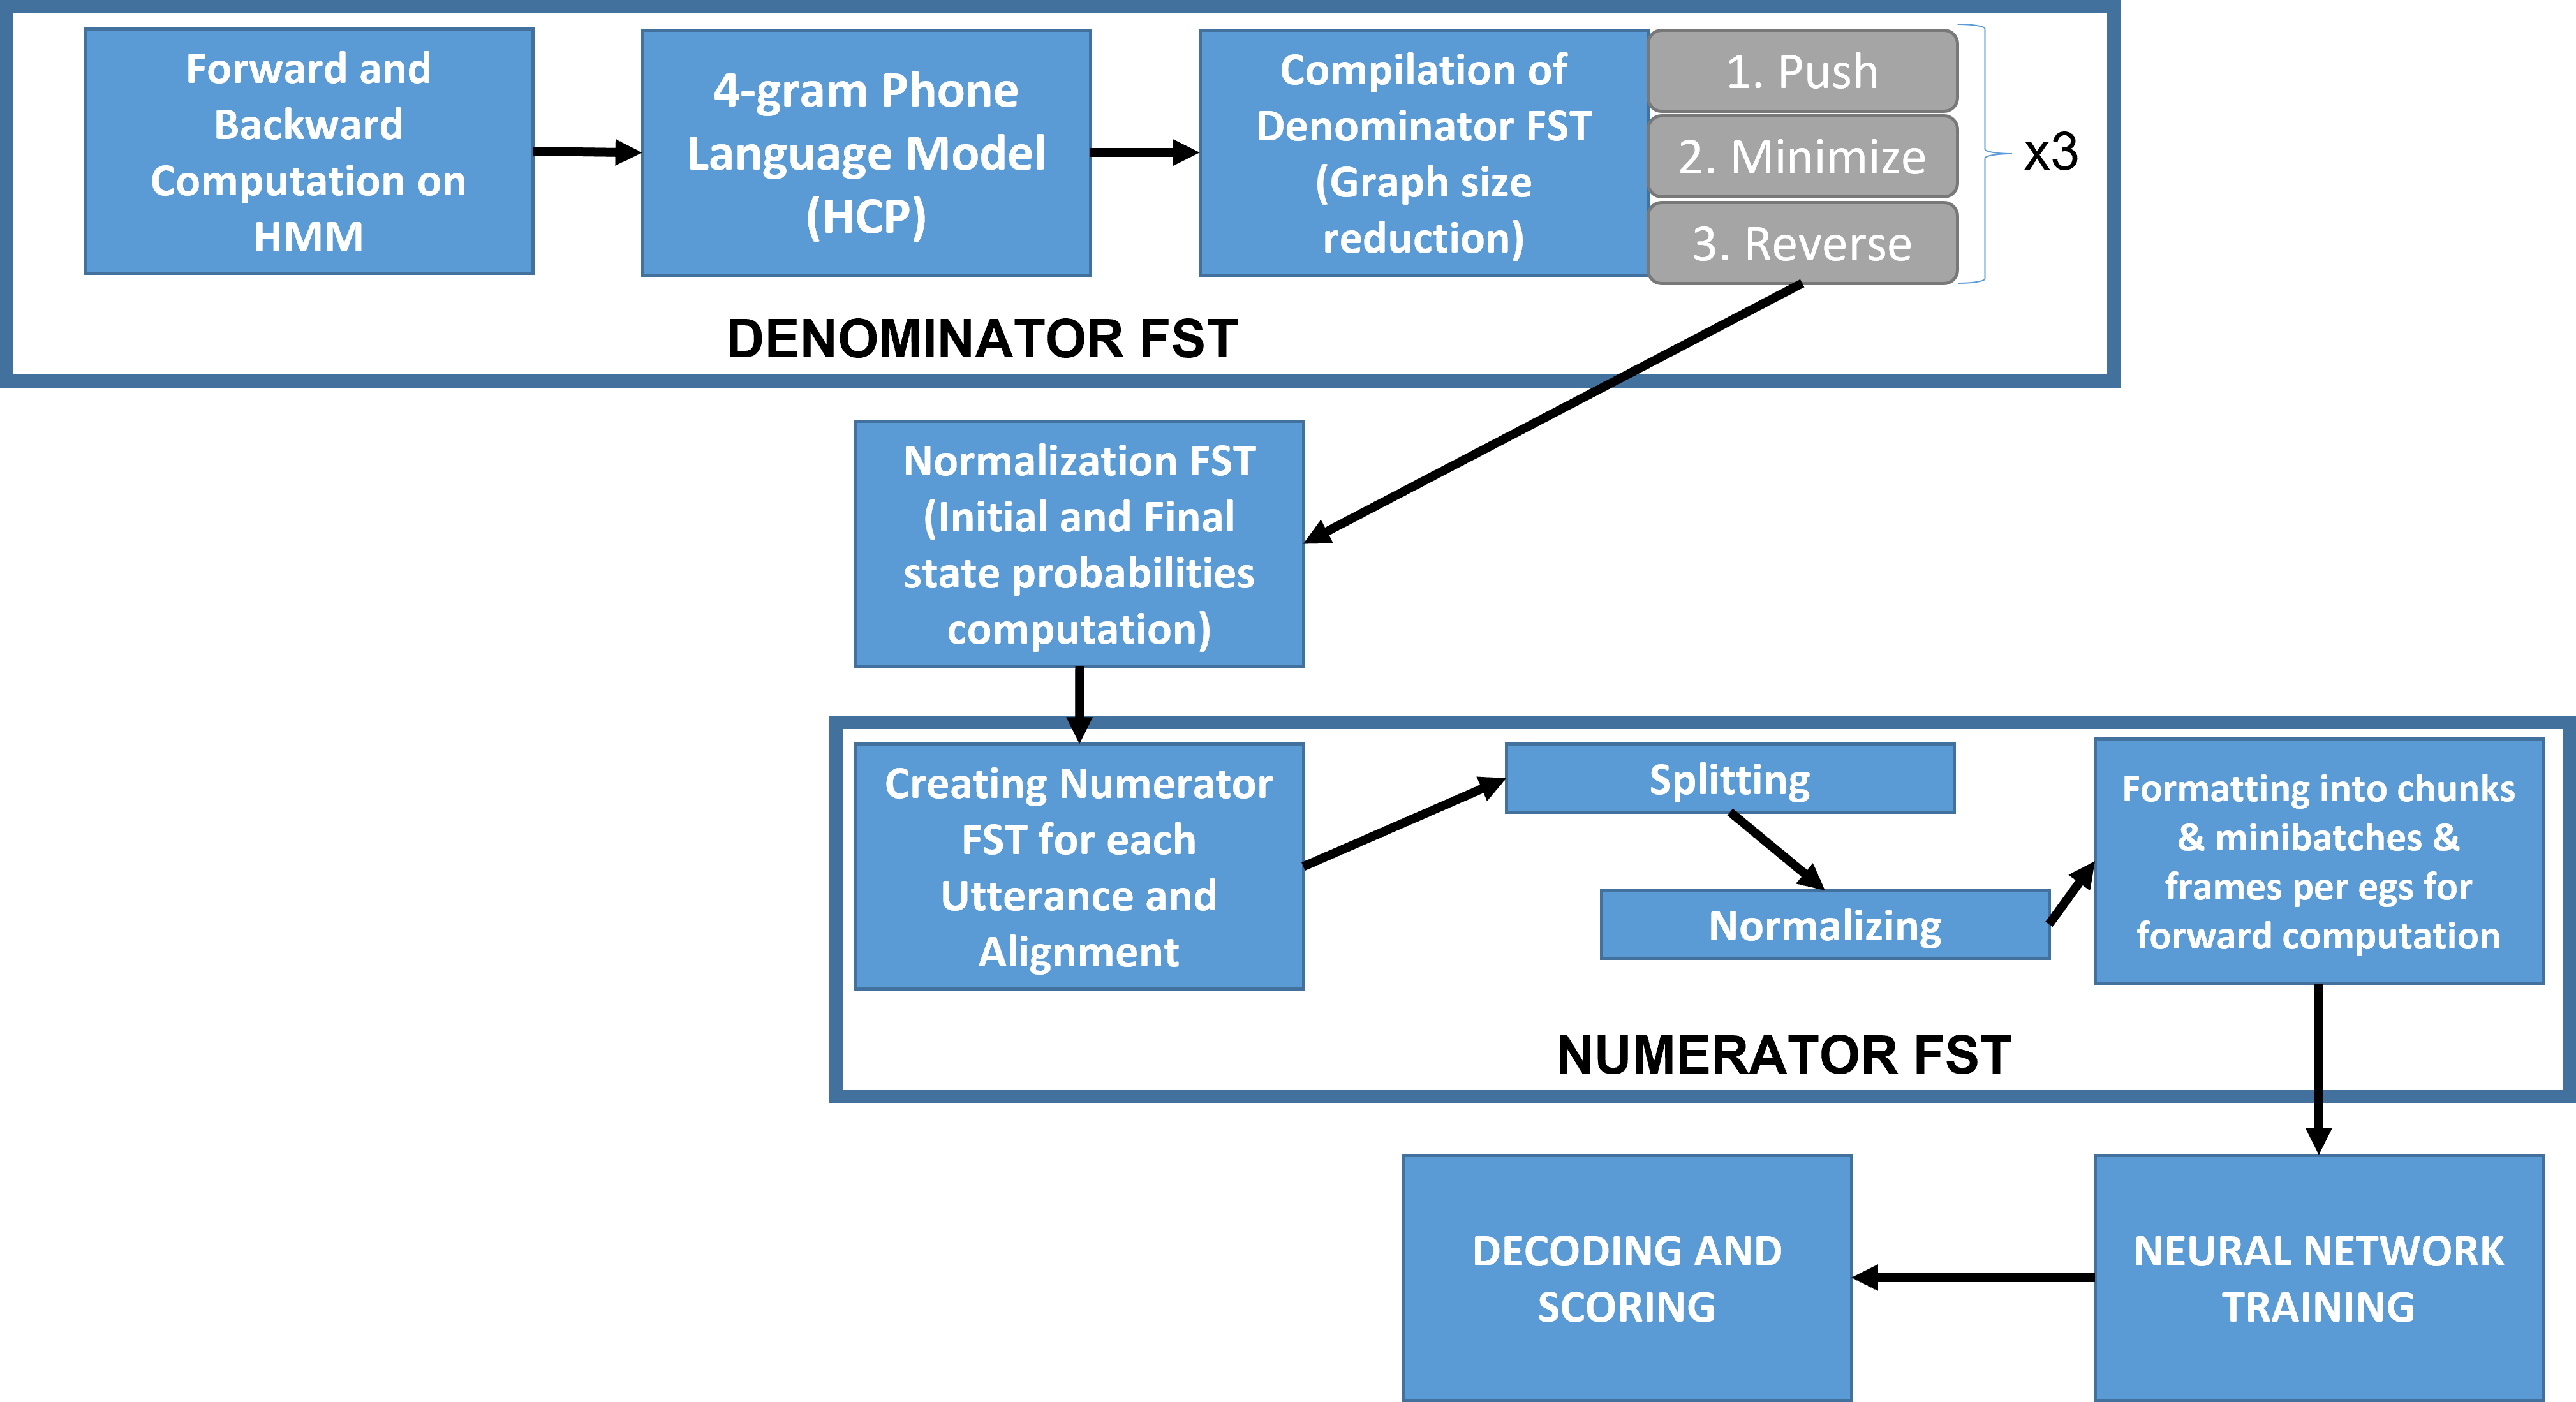
\includegraphics[width=0.8\textwidth]{img/ChainTrg.png}
    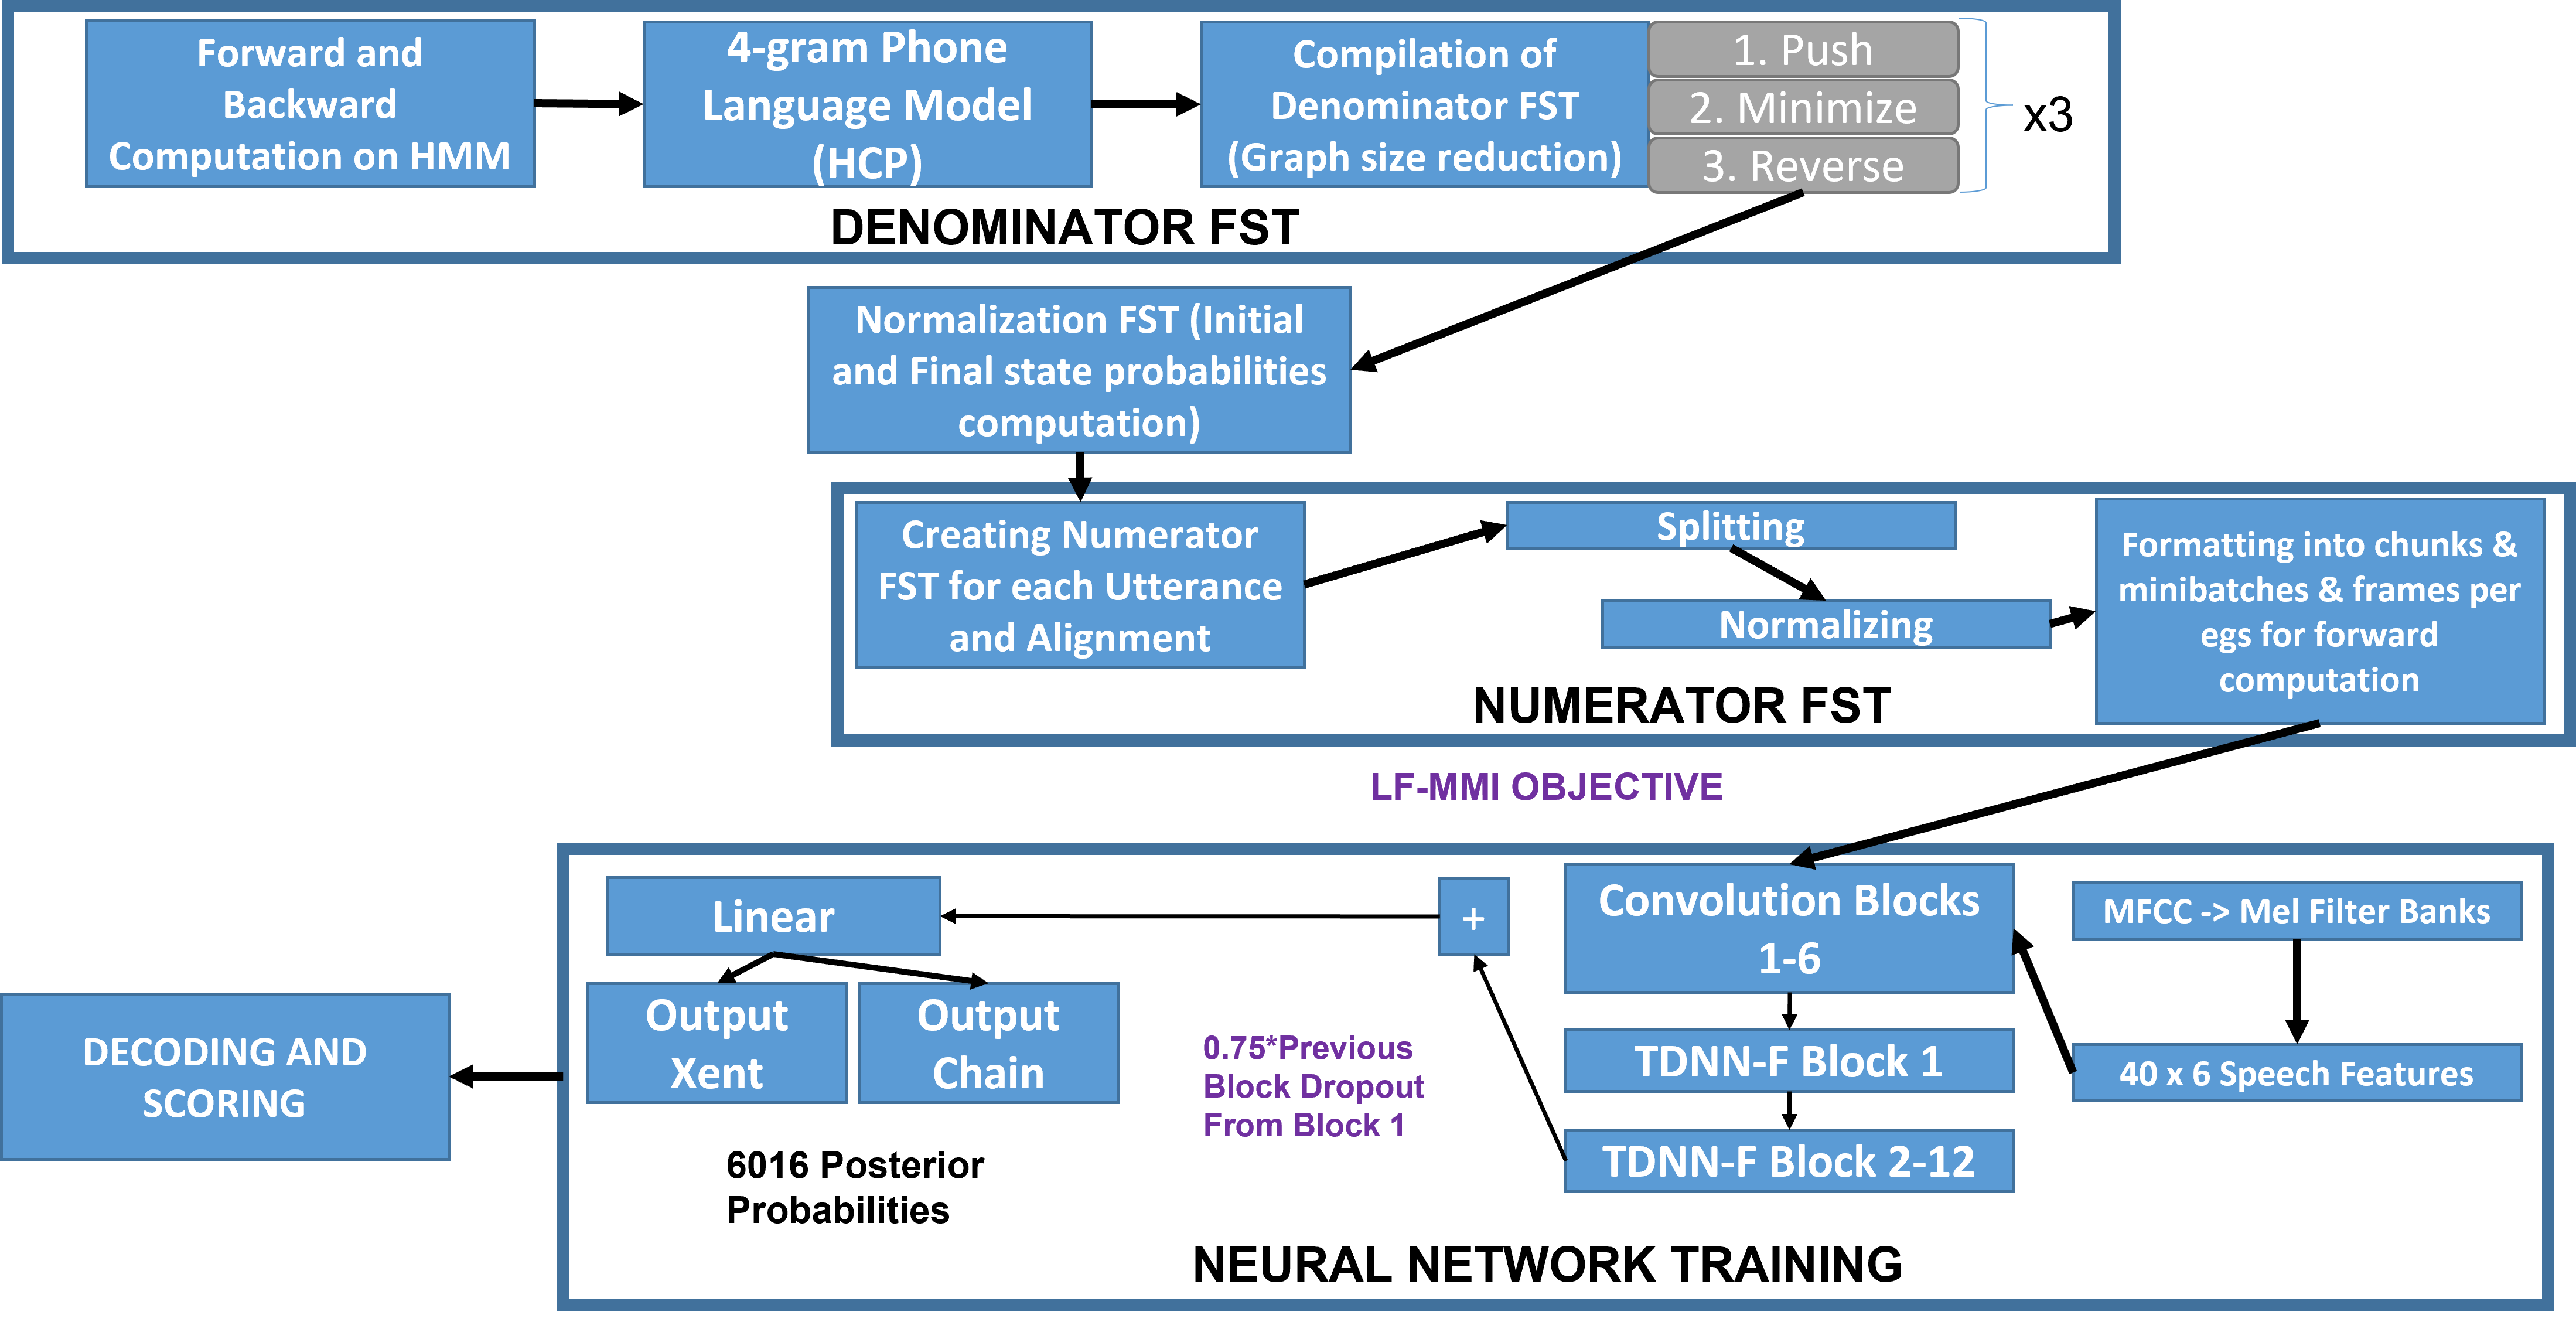
\includegraphics[width=0.95\textwidth]{img/ChainModel-Detail.png}
    \caption{Chain or LFMMI Training Outline}
    \label{fig:Chain-Training-outline}
\end{figure}
 

\subsection{LFMMI Objective Function}

The chain model or Lattice Free Maximum Mutual Information Model is like a typical HMM-DNN with one third of the traditional frame rate at the DNN's output. The DNN's input features are at the original frame rate of 100 frames per second since CNNs, LSTMs, TDNNs, etc have recurrent connections or splicing inside them and are they are not purely feed-forward nets. This model uses a frame-level objective i.e. log-probability of the correct phone sequence. 

The initial probabilities of the corresponding FSTs requires re-adjustment since the utterances are split into 1.5 second slices. Utterances are sliced off often from the middle. This initial probability is calculated by performing the HMM for 100 time-steps beginning with the initial state and then averaging the distribution of states over these 100 time-steps.

The HMM should be traversable in a single transition of a model at the normal frame rate instead of three transitions. A single-occurring state is present in the current topology, followed by a state that can appear zero or more times. Similar to GMM-based models, the state-clustering is obtained, but with a different topology for converting the alignments to the new topology and frame-rate.

Chain model training process is a lattice-independent version of MMI, in which a forward-backward algorithm over an HMM created from a phone-level decoding graph is used to obtain the denominator state posteriors. A similar forward-backward algorithm, but restricted to transcript-corresponding sequences, is used to obtain the numerator state posteriors.

Like MMI, numerator and denominator 'occupation probabilities' computed and the difference between the two is used in the derivative computation. Normalization of DNN outputs is no longer required to sum to one on each frame as it makes no difference. A modified HMM topology is used because of frame rate of 1 frame per 30 ms \cite{daniel_povey_kaldi_nodate}. The gradient descent requires computation of two sets of posterior probabilities for: 
    \begin{enumerate}
    \item Numerator graph specific to an utterance 
    \item Denominator graph encoding every possible word sequences which will be the same for all utterance in LF-MMI unlike the lattice-based MMI. 
\end{enumerate}

Forward and backward computations are computed in these two situation:
\begin{enumerate}
    \item During training time for computation of numerator FST and denominator FST state occupancies which are the product ($\alpha \beta$) of any states obtained using forward ($\alpha$) and backward algorithm ($\beta$) respectively.
    \item During Testing time Veterbi Decoding while pruning FST some type of forward looking is required to avoid pruning paths that can have higher probability at later stage using $\beta$ as a proxy look-ahead. 
\end{enumerate}

The forward and backward computations for numerator FST are on CPU since they are small and for denominator FST, these computations are performed on GPU but not on log domain since computation of log several times slows the process. The objective function values can occasionally become bad for which we keep the objective function within [-30,30] range \cite{raj_experiments_nodate}. To reduce the maximum memory usage, the denominator computation is performed before the numerator. This algorithm is also prone to numeric overflow and underflow, which can be avoided by multiplying the emission probability of the frame by the normalisation factor $\frac{1}{alpha(t)}$.

Now we will explore the key processes in the chain model.

\subsubsection{Forward and Backward Computation of Denominator FST} 

A derivative of the form \textit{"numerator occupation probability - denominator occupation probability"} for each output index or pdf-id of the Neural Network is computed and propagated back into the Neural Network. 
    \begin{itemize}
        \item Forward-backward over an HMM for the denominator is done as part of the computation. 
        \item The labels or pdf-ids are associated with the arcs rather than the states because it is represented as a finite state acceptor. 
        \item Although this is not a true traditional HMM, it is still regarded as one due to the use of the forward-backward algorithm (denominator FST) to obtain posteriors.
    \end{itemize}    
\subsubsection{Phone LM \& Denominator FST} 
Building Phone LM is first step to build the denominator FST. 
    \begin{itemize}
        \item Phone LM is derived from phone alignments in training data making it an un-smoothed language model, which means there is no reverting to lower order n-grams. 
        \item Transition to some LM states that are removed go to lower order n-gram states. Smoothing is avoided to reduce number of arcs in compiled graph after phonetic context expansion.
        \item There is a requirement for maintenance of 2-phone history which is why a 4-gram language model is used for chain training and we never prune LM states below the trigram level which not pruned because any sparsity in which trigrams are permitted tends to reduce the size of the compiled graph.
    \end{itemize}

%In addition to the number of states dictated by the no-prune trigram rule, we have a selectable number (e.g., 2000) of 4-gram language model states to be retained (the rest are identified with the corresponding trigram state), and the ones we select are determined in a way that maximises the training-data likelihood. To maximise the training-data likelihood, all probabilities are estimated. 

%It is worth noting that if our phone LM was just a simple phone loop (i.e. a unigram), it would be expanded to triphones due to phonetic context effects, but it would contain arcs for all possible trigrams. So any sparsity obtained by using the un-pruned trigram model is a bonus. Empirically, an un-smoothed trigram LM is what expands to the smallest possible FST; and pruning some of the trigrams results in little or no WER improvement while increasing the size of the compiled FST (at least on 300 hours of data expanded 3-fold with speed perturbation; on less data it might help). 

%The phone-LM perplexities for the various models we tried on the Switchboard setups ranged from 5 to 7; the phone-LM perplexity with our chosen configuration (4-gram, pruned to trigram for all but 2000 states) was around 6. Lower phone-LM perplexity did not always result in better WER of the trained system; for conventional (word-based) MMI training, an intermediate strength of language model seemed to work best.

\subsubsection{Compilation of the denominator FST} 
Phone LM is expanded into an FST with pdf-ids as the arcs, through a process akin to a normal decoding-graph compilation, but without using a Lexicon, at end of which the transition-ids are converted to pdf-ids. 
    \begin{itemize}
        \item The difference lies in graph size minimization because the standard recipe calls for determination and minimization. 
        \item This procedure it's variants with disambiguation symbols, do not allow graph size reduction which is why the graph-minimization procedure is three repetitions of: 
        \begin{enumerate}
            \item Push
            \item Minimize
            \item Reverse (The terms 'push' and 'reverse' refer to reversing the directions of arcs and swapping initial and final states.)
        \end{enumerate}
    \end{itemize}
    
\subsubsection{Initial \& Final Probabilities} 
A starting state and final probabilities for every state are produced by the graph-creation process naturally. 
    \begin{itemize}
        \item These are not the states used in the forward-backward procedure because these probabilities apply to utterance boundaries but it is trained on fixed-length chunks of utterance which is usually 1.5 seconds. 
        \item Constraining the HMM to the initial and final states at these arbitrarily chosen cut points is not appropriate. 
        \item For each state instead, we use: 
        \begin{itemize}
            \item Derivation of Initial Probabilities from fixed iterations of HMM-running 
            \item Averaging the probabilities
            \item Final probabilities = 1.0 for each state.
        \end{itemize}        
    \end{itemize}    

\subsubsection{Normalization FST} 
The initial and final probabilities are applied to the initial and final frame as part of the computation in the denominator forward-backward process. 
    \begin{itemize}
        \item Normalisation FST is a version of the denominator FST with these initial and final probabilities. 
        \item Epsilon ($\epsilon$) arcs are used to simulate initial probabilities since they are unsupported by FSTs. 
        \item Probabilities will then be added to normalization FST using Normalization FSTs.
    \end{itemize}   
    
\subsubsection{Numerator FSTs} 
A numerator FST for each utterance is generated to prepare the training process, which encodes the supervision transcript along with the transcript alignment to force similarity to reference alignment, allowing a little deviation, acquired from a base-line system . 
    \begin{itemize}
        \item A phone is allowed  in the lattice alignment to occur 0.05 seconds prior or after its start and end positions, respectively. 
        \item Alignment details must be included as training is done on fixed-length utterance segments rather than complete utterances, i.e. If we know where the transcript aligns, we can split the utterance into pieces, which is important for GPU-based training.
        \item Rather than enforcing a specific pronunciation of the training data, a lattice of alternative pronunciations of the training data is used, which is generated by a lattice-generating decoding procedure that uses an utterance-specific graph as our reference decoding graph, generating all pronunciation alignments within a beam of the highest-scoring pronunciation.
    \end{itemize}

\subsubsection{Splitting the numerator FST} 
Fixed sized utterances of 1.5 seconds length are used, necessitating division of the numerator FSTs into fixed-size segments. This is simple because the numerator FSTs remembers and encode time-alignment information and  have a structure that allows association of any FST state with a specific frame index. At this time, there are no costs in the numerator FST. It is only viewed as encoding a path constraint, so there is no need to decide how to split up the costs on the paths.

\subsubsection{Normalizing the numerator FSTs} 
Normalisation FST is merged with split-up pieces of numerator FST to ensure that the denominator FST costs reflect in the numerator FST which in turn ensures that objective functions are never positive and making their interpretation easier. 

This prevents the objective function from ever decreasing by preventing the numerator FST from having state sequences that the denominator FST would find unacceptable while also protecting against the possibility of numerator FST containing state sequences not accepted by denominator FST, which allows the objective function to indefinitely increase. 

The Lattices may contain n-gram phone sequences which were not seen in training since Phone LM has no smoothing and is estimated from 1-best alignments. Normalization process infrequently generates empty FSTs which can happen when: 
        \begin{itemize}
            \item The lattice consists of tri-phones absent in the 1-best alignment that was used to train the Phone LM and, 
            \item No alternative paths are available at that point in the lattice to compensate for the resultant failed paths which is a possibility because the lattice-producing alignment and 1-best alignment selected different pronunciations of the same word which is why These utterance fragments are simply discarded.
        \end{itemize}

The initial probabilities are now have different values which becomes a problem for chunk-level FSTs. To approximate this, the HMM running is done for a few iterations and then the probabilities are averaged to be used as the initial probability of any state. Thus Normalization FST seems to work despite being a crude type of approximation. The numerator FST is composed with the normalization FST for following reasons: 
       \begin{enumerate}
            \item Ensure that objective function value is always negative for easier interpretation. 
            \item Ensure that the numerator FST is free of sequences not permitted by the normalisation or denominator FST, which commonly happens because the sum of the overall path weights for such sequences is dominated by the normalization FST part. %\cite{raj_experiments_nodate}.
        \end{enumerate}

\subsubsection{Format of the numerator FSTs} 
Pdf-ids can not be directly used as weighted acceptors in the numerator FSTs because they could be zero which is treated differently by Open-Fst i.e. as epsilon. Hence, numerator FSTs' weighted acceptors correspond to \textit{"pdf-ids + 1"}. Instead of storing an array of separate numerator FSTs, they are appended together to form a longer FST when mini-batches are formed. This enables a single forward-backward algorithm to be applied to every utterance in the mini-batch, directly calculating the total numerator log-probability. 

\subsubsection{Chunks-Size} 
The number of output frames for each chunk of data that we analyse and evaluate during training or decoding is known as the chunk-size.
    \begin{itemize}
        \item There is a mechanism for variable chunk sizes that permits reasonably large chunks while preventing data loss from files that are not exact multiples of the chunk size. 
        \item The first specified chunk size is called primary chunk-size which is unique because we can choose no more than two non-primary chunk sizes for any given utterance and the remaining chunks must be of the primary chunk size. Determining the optimal split of a file of a given length into chunks is made easier by this restriction, allowing the biasing of chunk-generation to chunks of a specific length.
        \item The number of frames per chunk influences the speed or latency trade-off but not the results.
    \end{itemize}    

\subsubsection{Mini-Batches} 
A larger mini-batch size is generally more efficient because it interacts well with optimizations used in matrix multiplication code, particularly on GPUs, but it can lead to update instability if it is too large and the learning rate is too high. %We used mini-batch of 64 based on our dataset scenario. %Size 512 for GPU-based training is recommended and was used.
    \begin{itemize}
        \item To reduce the size of the denominator FST for training on the GPU training is done on 1 to 1.5 seconds chunks, instead of the complete utterance. However, the transcript needs to be broken up to do this and 1-second chunks may not coincide with word boundaries.
        \item Utterances are divided into given fixed-length chunks of speech to train on mini-batches of length 1.0 seconds. 
        \item Shorter utterances are removed, while longer utterances are divided into chunks with small gaps or overlaps between them.
        \item The acoustic models usually require left or right frames for acoustic context which is added but the context is added after the chunks have been determined. 
        \item Usually the mini-batch size is a power of two, and is possibly limited by GPU memory constraints. We used 64 mini-batches based on our data-set. 
        \item The alpha probabilities in forward-backward computation consume the most GPU memory. 
        \item After the 3-fold sub-sampling, we have 50 time steps with a 1 second chunk.
    \end{itemize}

\subsubsection{Frames per Egs} 
The entire data-set is randomised at the frame level for the most basic types of networks, such as feed-forward networks or TDNNs trained with the cross-entropy objective function, and training is done on one frame at a time. 
    \begin{itemize}
        \item Data is pre-randomized at the frame level in order for the training jobs to mostly do sequential I/O. 
        \item If 10 frames are needed each of left and right context or when generating the training examples, there may be a requirement of increasing the amount of data by a factor of 20. This issue is resolved by including labels for time value ranges i.e. \textit{frames-per-eg} value, and include enough left/right context that we can train on any of those given frames. If that value is suppose 10, any given training job will pick one of those 10 frames to train on. 
        \item Based on our data-set and scenario we used values of 150,110,100,30 for \textit{Frames per Eg}.
    \end{itemize}
 

%We used Frames per e.g = 150, 110, 100, 30 due to varying size of our data-set and 10 Epochs and Initial Number of jobs =3 and Final Number of jobs= 16 for trainer optimization.  

%https://kaldi-asr.org/doc/dnn2.html
%https://kaldi-asr.org/doc/chain.html

\subsubsection{Avoiding Over-fitting}
To avoid over-fitting, LF-MMI uses following techniques \cite{raj_experiments_nodate}:
\begin{enumerate}
    \item \textbf{L-2 regularization on neural network outputs:} This forces the weight parameters to decay or approach zero but become exactly zero. It is also called Ride Regression or Weight Decay. Smaller weight parameters makes neurons negligent which reduces neural network complexity and hence, over-fitting. 
    \item \textbf{Separate classifier Output Layers:} LFMMI uses two separate output layers for classifier, one trained with MMIE and the other with cross-entropy so that the overlapped layers will be trained with both objectives to reduce over-fitting that is caused by a single objective.
    \item \textbf{Multitask training with the cross-entropy objective:} The forward probabilities at each time step in the numerator graph are used as soft targets instead of the usual hard targets.
    \item \textbf{Leaky HMM:} This permits small transition probability between any two states is allowed allowing for gradual context forgetting. %https://m-wiesner.github.io/LF-MMI/
\end{enumerate}

\begin{figure}
    \centering
    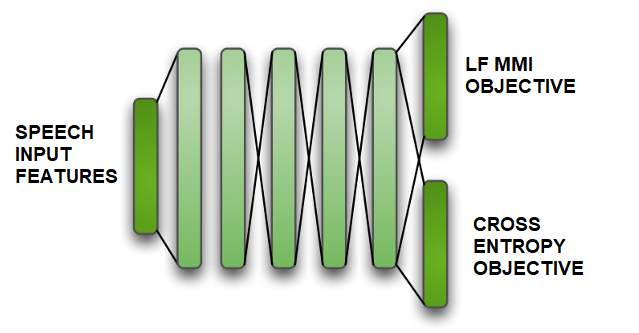
\includegraphics[width=0.7\textwidth]{img/LFMMI-crossent.png}
    \caption{LFMMI input objectives}
    \label{fig:LFMMI-INPUT}
\end{figure}

\subsection{Neural Network Training with CNN-TDNN}

For The Neural Network training part in Figure \ref{fig:Chain-Training-outline} the 1500ms speech segments with 40 Mel filter-banks features and 200 iVectors are the input and structure of the network is CNN-TDNN as shown in Figure \ref{fig:CNNTDNN-Layout}. The LF-MMI here is the training objective i.e. they define how the weights are set during the training. We will now explore this further.  

We will use CNN-TDNN for Neural Network training because various reports like \cite{abdel-hamid_convolutional_2014}, \cite{zorila_investigation_2019}, \cite{biswas_semi-supervised_2019}, \cite{noauthor_tdnn_nodate} \cite{georgescu_kaldi-based_2019} and \cite{kreyssig_improved_2018} suggested that CNN-TDNN perform better than simple TDNN, however, the former requires relatively a bit more computing power \cite{georgescu_performance_2021} which is very minor. 

\cite{georgescu_kaldi-based_2019} conducted a comparative test of various TDNN based architectures on RSC and SSC Datasets. The RSC corpus consisted of read speech utterances recorded in a silent environment whereas SSC corpus comprised of spontaneous utterances, gathered from the Romanian media broadcasts of which some were clean, recorded in a silent environment, while the others contained background noise. Their results showed that CNN-TDNN performed better with the noisy SSC corpus which made it perfect for our use.

The performance of various HMM-DNN and E2E architectures were investigated by \cite{georgescu_performance_2021}, which shows that it performed almost equally to TDNN in a clean data-set of Librispeech but on "other" data-set of LibriSpeech, CNN-TDNN actually performed better than pure TDNN and E2E models. 

CNN-TDNN is a variant of simple TDNN model and it is part of a multi-component system comprising of a hybrid HMM-TDNN based acoustic model, a phonetic model and an n-gram language model. Optionally for re-scoring, a complex n-gram or NN-based LM can be used. In Chain or LFMMI model with CNN-TDNN, 4-gram model is used. 

Mel-filter-banks are used in this implementation instead of MFCCs, in terms of network input features. Here the final features are organized as a matrix unlike simple TDNN where the input features are represented as a vector. 

The input in the CNN-TDNN network comprises of two feature types organized in a 40x6 matrix of speech features \cite{georgescu_performance_2021}: 

\begin{enumerate}
    \item 40-dimensional Mel-filter-banks extracted from 25 ms length frames
    \item 200-dimensional and 10 ms i-vectors-shift calculated from chunks of consecutive 150 frames
\end{enumerate}

The feature extraction procedure and organization of these features are shown in Figure \ref{fig:CNN-TDNN-INPUT}. TDNNs are one dimensional or temporal CNNs whereas CNN works on time as well as frequency dimension. Note that unlike TDNN, CNN-TDNN requires Mel filterbanks instead of MFCCs because the CNN layer needs to have a meaningful non-time dimension to operate on which is why we want our signals to be in  frequency space or dimension. They are still dumped to disk as MFCCs during the NN extraction and training process but the DCT part of MFCC is inverted or reversed to get Filterbanks. 

The neural network component acoustic model of CNN-TDNN resembles TDNN, the key difference being placing of few CNN layers prior to the time-delay layers, acting as a front-end block. The input for Conv. Block 1 are three matrices of speech features i.e. the features for the current, previous, and next acoustic frames, or a feature volume of 6 x 40 x 3 equivalently. Time and feature space convolutions are performed using 64 filters of size 3x3, and the output is 64 x 40 x 1 volume. %\cite{georgescu_performance_2021}

The Second Convolutional Block's input comprises of three time consecutive volumes as the first Convolutional Block's output, that are spliced together to form the 64 x 40 x 3 feature volume. The second Convolutional block performs time and feature space convolutions with another 64 3x3 filters and gives 64 x 40 x 1 volume as output. 

In Convolutional Blocks 3–6 more filters are used, ranging from 128 to 256, while feature volume size is kept constant by reducing the height from 40 to 20, and then to 10, finally generating a 2560-dimensional output that is passed on to the next time-delay blocks from whereon the processing is same as TDNN.

Convolutional layers have the property of annihilating small variations in the spectral domain due to their structure provided by local connectivity, weight sharing, and pooling \cite{georgescu_performance_2021}. These variations are induced by both the speaker and the acoustic environment in which the speech takes place. 

The Convolution Block 2 input has three time consecutive volumes as the Convolution Block 1 output, spliced together to form the 64 x 40 x 3 feature volume. The second convolutional block performs time and feature space convolutions with another 64 3x3 filters and gives a 64 x 40 x 1 volume as output.

Conv. Blocks 3–6 more filters ranging from 128 to 256, while maintaining the size of the feature volume by reducing the height from 40 to 20, and finally to 10. The convolutional blocks generate a 2560-dimensional output that is passed on to the following time-delay blocks. %\cite{georgescu_performance_2021} 

The possible reason why adding CNNs before TDNN improves performance in noisy environment is that TDNNs are basically time-dilated 1 Dimensional CNNs and if the input features are noisy, having a few CNN layers (2D CNN) at the input would help the model learn some non-linear transformations which can reduce the effect of the noise on speech input. %(think of the D dimension in the input).

Front End CNN Blocks are followed by 12-blocks of factored TDNN (TDNN-F). TDNN-F Block 1 processes the current time frame only, while the rest perform temporal convolution over $t-3$, $t$, and $t+3$  time indexes. The linear layer is formed by splicing the input vectors at time indexes $t-3$ and $t$ are spliced together to form the linear layer. The affine layer is formed by splicing the input vectors at time indexes $t$ and $t+3$.  

TDNN employs a sub-sampling technique to compute hidden activations only at specific time steps which avoids redundancy because the large overlap of contexts leads to highly correlated neighbouring activations. A larger context on the left side is usually found to be optimal for online decoding. This way, Model size and training time are reduced. 

TDNN with sub-sampling increases training speed and are therefore faster than LSTM. They learn local correlations between speech frames. Bottleneck layers, which are initialized by Singular value decomposition (SVD), constrains rank of weight matrices which help in regularization and reduces number of Multiplications $M x N -> (M+N) x R$. 

The TDNN network's sub-sampling mechanism is similar to a convolutional operation that allows gaps in the convolutional filter which is another network variant based on the purely TDNN approach, with a couple of stacked convolutional layers added before with a primary function to further process acoustic features and act as a feature processing front-end. These additional layers reduce spectral and temporal variability. 

The output blocks use cross-entropy and chain loss functions in TDNN and CNN-TDNN both. The CNN-TDNN and simple TDNN architectures have identical Neural Network output blocks, which are represented by 6016-dimensional posterior probabilities of acoustic states, while the language model of 200K words provides the system output. 

We used 10 Epochs with 10 hidden layers while reducing the learning rate geometrically from initial learning rate of 0.00015 to the final learning rate of 0.00015, and then keep it fixed at –final-learning rate, for extra number of 5 epochs. Maximum parameter change value was 2.0 along with Initial Number of jobs =3 and Final Number of jobs= 16 for trainer optimization. We provided the forced alignments from HMM-GMM Tri-phone to our LF-MMI or chain CNN-TDNN pipeline. The training resulted in 5.2\% WER and 20.45\% SER.

\section{Decoding}
\label{sub:decoding}

Decoder algorithms efficiently search the hypothesis space by combining AM and LM predictions and output the most likely text-string for a given speech input file. Decoder aims to combine these various models, given the input sentence, to estimate the likelihood of a sound sequence already observed in the speech database. The system then searches through all sentences in the space, selecting the sentence with the highest probability of being the input source sentence. The solution for the \textit{search} or \textit{decoding problem} for a massive set of all English sentences requires an efficient algorithm which only searches through sentences which are more likely to match the input instead of searching through all possible English sentences.

After training, we need to analyze the model by testing it with unseen data during training. For that we decode the graph files which are produced at end of each training i.e. mono-phone, tri-phone and CNN-TDNN. This is then scored and evaluated.

\subsection{HMM-GMM Mono and Triphone Decoding}
Weighted Finite State Transducers are used in the HMM-GMM decoding algorithm, which provides graph operations for acoustic modelling. These decoding graphs are assigned numerical values known as pdf-ids that represent context-dependent states. 

Pdf-ids are numerical values of context dependent states given by decoding graphs formed by the decoding algorithms which uses WFSTs to provide graph operations used in acoustic modelling. WFST are used in HMM-GMM models and can also be used along with Deep Neural Network Classifiers.

Since different phones can have the same pdf-ids, Transition-ids are used to encode phone member pdf-ids and use arc (transition) within the topology specified for that phone. Thus, decoding is carried out on these decoding graphs HCLG, which are built from simple FST graphs. %HCLG %\cite{patil_automatic_2016}. 
\vspace{11pt}

\begin{center}
HCLG = H ◦ C ◦ L ◦ G    
\end{center}
\vspace{11pt}

The ◦ symbol denotes associative binary operation of composition on FST. \textit{H} for HMM state graph or definitions, \textit{L} for Language Models or Lexicon, \textit{G} is the acceptor which is used to encode the grammar and \textit{C}, the context dependency are combined to form HCLG (saved as HCLG.fst). 
\vspace{11pt}

\subsection{Chain Model Decoding}

The traditional "H ◦ C ◦ L ◦ G" is a composed transducer used to decode audio. This WFST can be integrated with the deep network classifier. It is a big complex network which can be trained like DNN or DL using back-propagation without the requirement of introduction of a lattice for denominator approximation. 

The numerator and denominator state sequences are encoded as Finite State Transducer corresponding to the HMMs. The objective function overall is the difference of these FSTs in log-space which is built as the HCLG FST decoder. 

The graph becomes too big to fit into GPU memory if the FST comprises of all possible word-sequences \cite{raj_experiments_nodate} which is why phone-level LM is used which contains fewer possible sequences. L-graph is not needed since we are using Phones instead of words. Phone-LM \textit{"P"} is a 4-gram model with no back-off less than 3-gram to ensure that tri-phones not seen in training are not generated and is constructed to minimize the graph size. Removing low-count 4-gram states completely will limit the number of states. 

Thus final graph will be \textit{HCP} file instead of \textit{HCLG}, where P = phone LM. Once HCP graph is composed, a different kind of \textit{graph minimization technique} is done by three iterations of the operations of Pushing the weights, graph minimization and reversing the arcs and swap initial and final states.

The numerator FST encodes utterance-specific alternate pronunciations of original utterance transcript. This lattice is converted into an FST with a 0.05-second error window from the phones' position in the lattice, limiting the time at which the phones can appear which is followed by conversion into an FST with labels that are pdf-ids or neural network outputs. This FST is used to extract fixed size chunks for training chunks in the denominator FST \cite{raj_experiments_nodate}.

The numerator FST contains the lattice for only one utterance, broken into chunks of fixed length, making it easily to calculate. It has H, C, and L without \textit{"G"} because the utterance is known. 

Phones can be taken at the numerator lattice's output and everything can be projected on the input to compose the numerator lattice with HCP. Since the numerator lattice changes with each utterance, this composition must be performed for each utterance. However, almost all paths in HCP are removed, and the final FST is very small because the numerator lattice is small and composition is analogous to intersection.

Key points in Chain Model Decoding are:
\begin{itemize}
    \item The graph is first constructed using a different and simple topology (\ref{fig:LFMMI-topology}) compared to a standard DNN, without any need of special action by the user. %as the graph-building script takes the topology from the 'chain' training script, which contains the correct topology.
    \item A self-loop-scale of 0.1 is used by default upon graph compilation which has an impact on how self-loop transition probabilities are handled and it usually performs better. 
    \item The exact same transition-probability scaling that we trained with must be used (due to the structure of LFMMI models) which is set to 1.0 for simplicity. As a result, we pass the -self-loop-scale 1.0 to the graph. %in utils/mkgraph.sh script.
    \item Division by the prior is not required in these models which is why there is no requirement of including the vector of priors in the model files. If the priors are not specified, the decoder skips the division by the prior.
    \item The default acoustic scale (0.1) usually used in decoding is not appropriate because the optimal chain model acoustic scale value is close to one, which is why it is set to 1.0 option and this value is then passed to decoding portion.
    \item The language model scale can only be searched by the scoring scripts in one incremental steps, which in typical configurations works when since the optimal LM scale range lies between 10 and 15, but it doesnot work for LM scale value close to 1.
    \item Although i-Vectors are used in this model but they have no relation with the chain models and there is no essential requirement for them. Mismatched length of utterances for training and testing tends to pose problems for ASR and Speaker Verification Tasks which i-vectors can solve. Experiments proved that even if the test utterances are short, training is on longer utterances gives better results \cite{sarkar_study_2012}.
\end{itemize}

\section{Scoring}

Scoring is done from decoding of the graphs that are generated as a result of HMM-GMM and Neural Network Training. There are some evaluation methods for ASR which we will explore first followed by scoring process.

\subsection{Selection of Evaluation Metric}
There is no single fixed method of evaluating ASRs, although Word Error Rate is the most popular mainstream metric for ASR Evaluation \cite{maglogiannis__2020}. Following are ASR scoring or evaluation metrics:

\subsubsection{Word Error Rate} 
WER is a popular ASR comparison index and is used to rate ASR performance accuracy by comparison of hypothesised and reference transcriptions. It expresses the distance between the reference series and ASR-producing word sequence.   
    \begin{itemize}
        \item The two-word sequences are first aligned using a string alignment algorithm based on dynamic programming. 
        \item After alignment, total substitutions (S), insertions (I) and deletions (D) are determined. The WER is calculated by dividing the number of errors (defined as substitutions, deletion and insertion) by the number of words (N) in the reference. 
        \item Substitution occurs when a word in the reference sequence is transcribed as a different word. When a word is completely absent from the automatic transcription, it is labelled as deleted. 
        \item Insertion is the appearance of a word in the transcription that has no counterpart in the reference word sequence. 
        \item WER is defined \cite{morris_wer_2004} as:
            \begin{equation}
                W.E.R = \frac{S+N+I+D}{N_{1}} =\frac{S+I+D}{H+S+D}   
            \end{equation}
            Total Entries = I, Total Deletions = D, Total Substitutions = S, Total Successes = H and Total Reference words = $N_{1}$
        \item WER has some drawbacks despite its popularity. It is not a true percentage because there is no upper limit. When S = D = 0 and we have two insertions for each input word, then I = $N_{1}$ (that is when the length of the results exceeds the number of words in the prompt), i.e. WER equals 200 percent. Thus, it only takes in comparison to other systems how good ASR performs. 
        \item WER may exceed 100 percent in noisy scenario because insertions are given far more weight than deletions.
    \end{itemize}

\subsubsection{Character or Phone Error Rate} 
Character Error Rate (CER) or Phone Error Rate (PER) is also used by some systems which evaluate how accurately the ASR system was able to understand the word at the phones/phoneme level e.g. differentiating "there" vs "their. The character error rate is also used to check the model's accuracy. Where S = Substitutions, D = Deletions, I = Insertions and N = Number of Letters in a Single Word, the formula for calculating the character error rate is as follows.:
        \begin{equation}
             C.E.R = (S + D + I) = N     
        \end{equation}
\subsubsection{Sentence Error Rate} 
SER is another metric that is sometimes used to assess the ASR performance. The percentage of sentences with at least one error can be calculated by SER.

\subsubsection{Word Information Lost} 
WIL is a simple approximation to the proportion of word information lost that avoids the issues associated with the RIL measure that was proposed many years prior.

\subsubsection{Relative Information Lost} 
RIL metric was not widely adopted because it is not as straightforward as WER and measures zero error for any one-to-one mapping between input and output words, which is not acceptable.

\subsubsection{Match Error Rate} 
MER is the proportion of I/O word matches (errors) i.e. the likelihood of a given match being incorrect. MER's ranking behaviour falls somewhere between WER and WIL \cite{morris_wer_2004}.
        \begin{equation}
            M.E.R = \frac{S+D+I}{N=H+S+D+I} =1-\frac{H}{N}   
        \end{equation}
        
\subsubsection{Position-Independent Error Rate} 
ASR Evaluation also correlates with the automatic metric PER (Position-Independent Word Error Rate). 
    \begin{itemize}
        \item When the words in the two sentences (hypothesis and reference) are compared, PER is always less than or equal to WER. 
        \item The set of words in a hypothesis sentence that do not appear in the reference sentence is referred to as the hypothesis per (Hper). 
        \item The set of words in a reference sentence that do not appear in the hypothesis sentence is denoted by reference PER (Rper), which is similar to recall. 
        \item Hper and Rper primarily aim to identify all words in the hypothesis that do not have a counterpart in the reference and vice versa \cite{maglogiannis__2020}.
    \end{itemize}
    
\subsection{Calculation of Scores}

We chose WER and SER for evaluation of our ASR. We had an option of using CER is also there but it is irrelevant for us since we are more concerned with the accuracy of words and sentences. The Urdu word \textit{"Janbaaz"} can be written as \textit{"Janbaaz"} or \textit{"Jaanbaz"} and will be spelled pretty much in the same way. As long as the overall word recognition is accurate and the sentences are accurately transcribed, our ASR is good for our requirement which is why we used WER and SER for our scoring.

The HMM-GMM part of the training produces HCLG file from which scoring is done based on chosen evaluation metric (as shown in previous subsection) by calculating insertions, deletions and substitutions from reference scripts.  

In the LF-MMI model, neural networks are a box that scores the gradient function's emission probability that we train. Every HMM state corresponds to pdf-id, and the neural network must provide a score for each pdf-id for each frame in the output \cite{ghahremani_investigation_2017}. 

Hence input frames chunk having width \textit{"w"}, the \textit{"N x w"} dimension matrix is the Neural Network output, where \textit{"N"} corresponds to total \textit{pdf-ids}. This matrix can be represented as an FST also called as scoring FST or sausage lattice, with nodes representing frames, arcs representing \textit{pdf-ids}, and weights on the arcs representing neural network scores. The Scoring FST is composed with HCP to get final total score.

The Scoring FST provides the acoustic score, and the graph provides the graph score. The neural network is trained with lattice posteriors generated by forced alignment using a trained GMM-HMM model \cite{raj_experiments_nodate}. The best HMM-GMM acoustic model (Triphone-3) is used to force-align the training data in order to produce high-quality alignments for the Neural Network model which in our case in CNN-TDNN.

\section{Speech To Text Interface} % (fold)
\label{sec:STT-interface}

\begin{figure}[h]
    \centering
    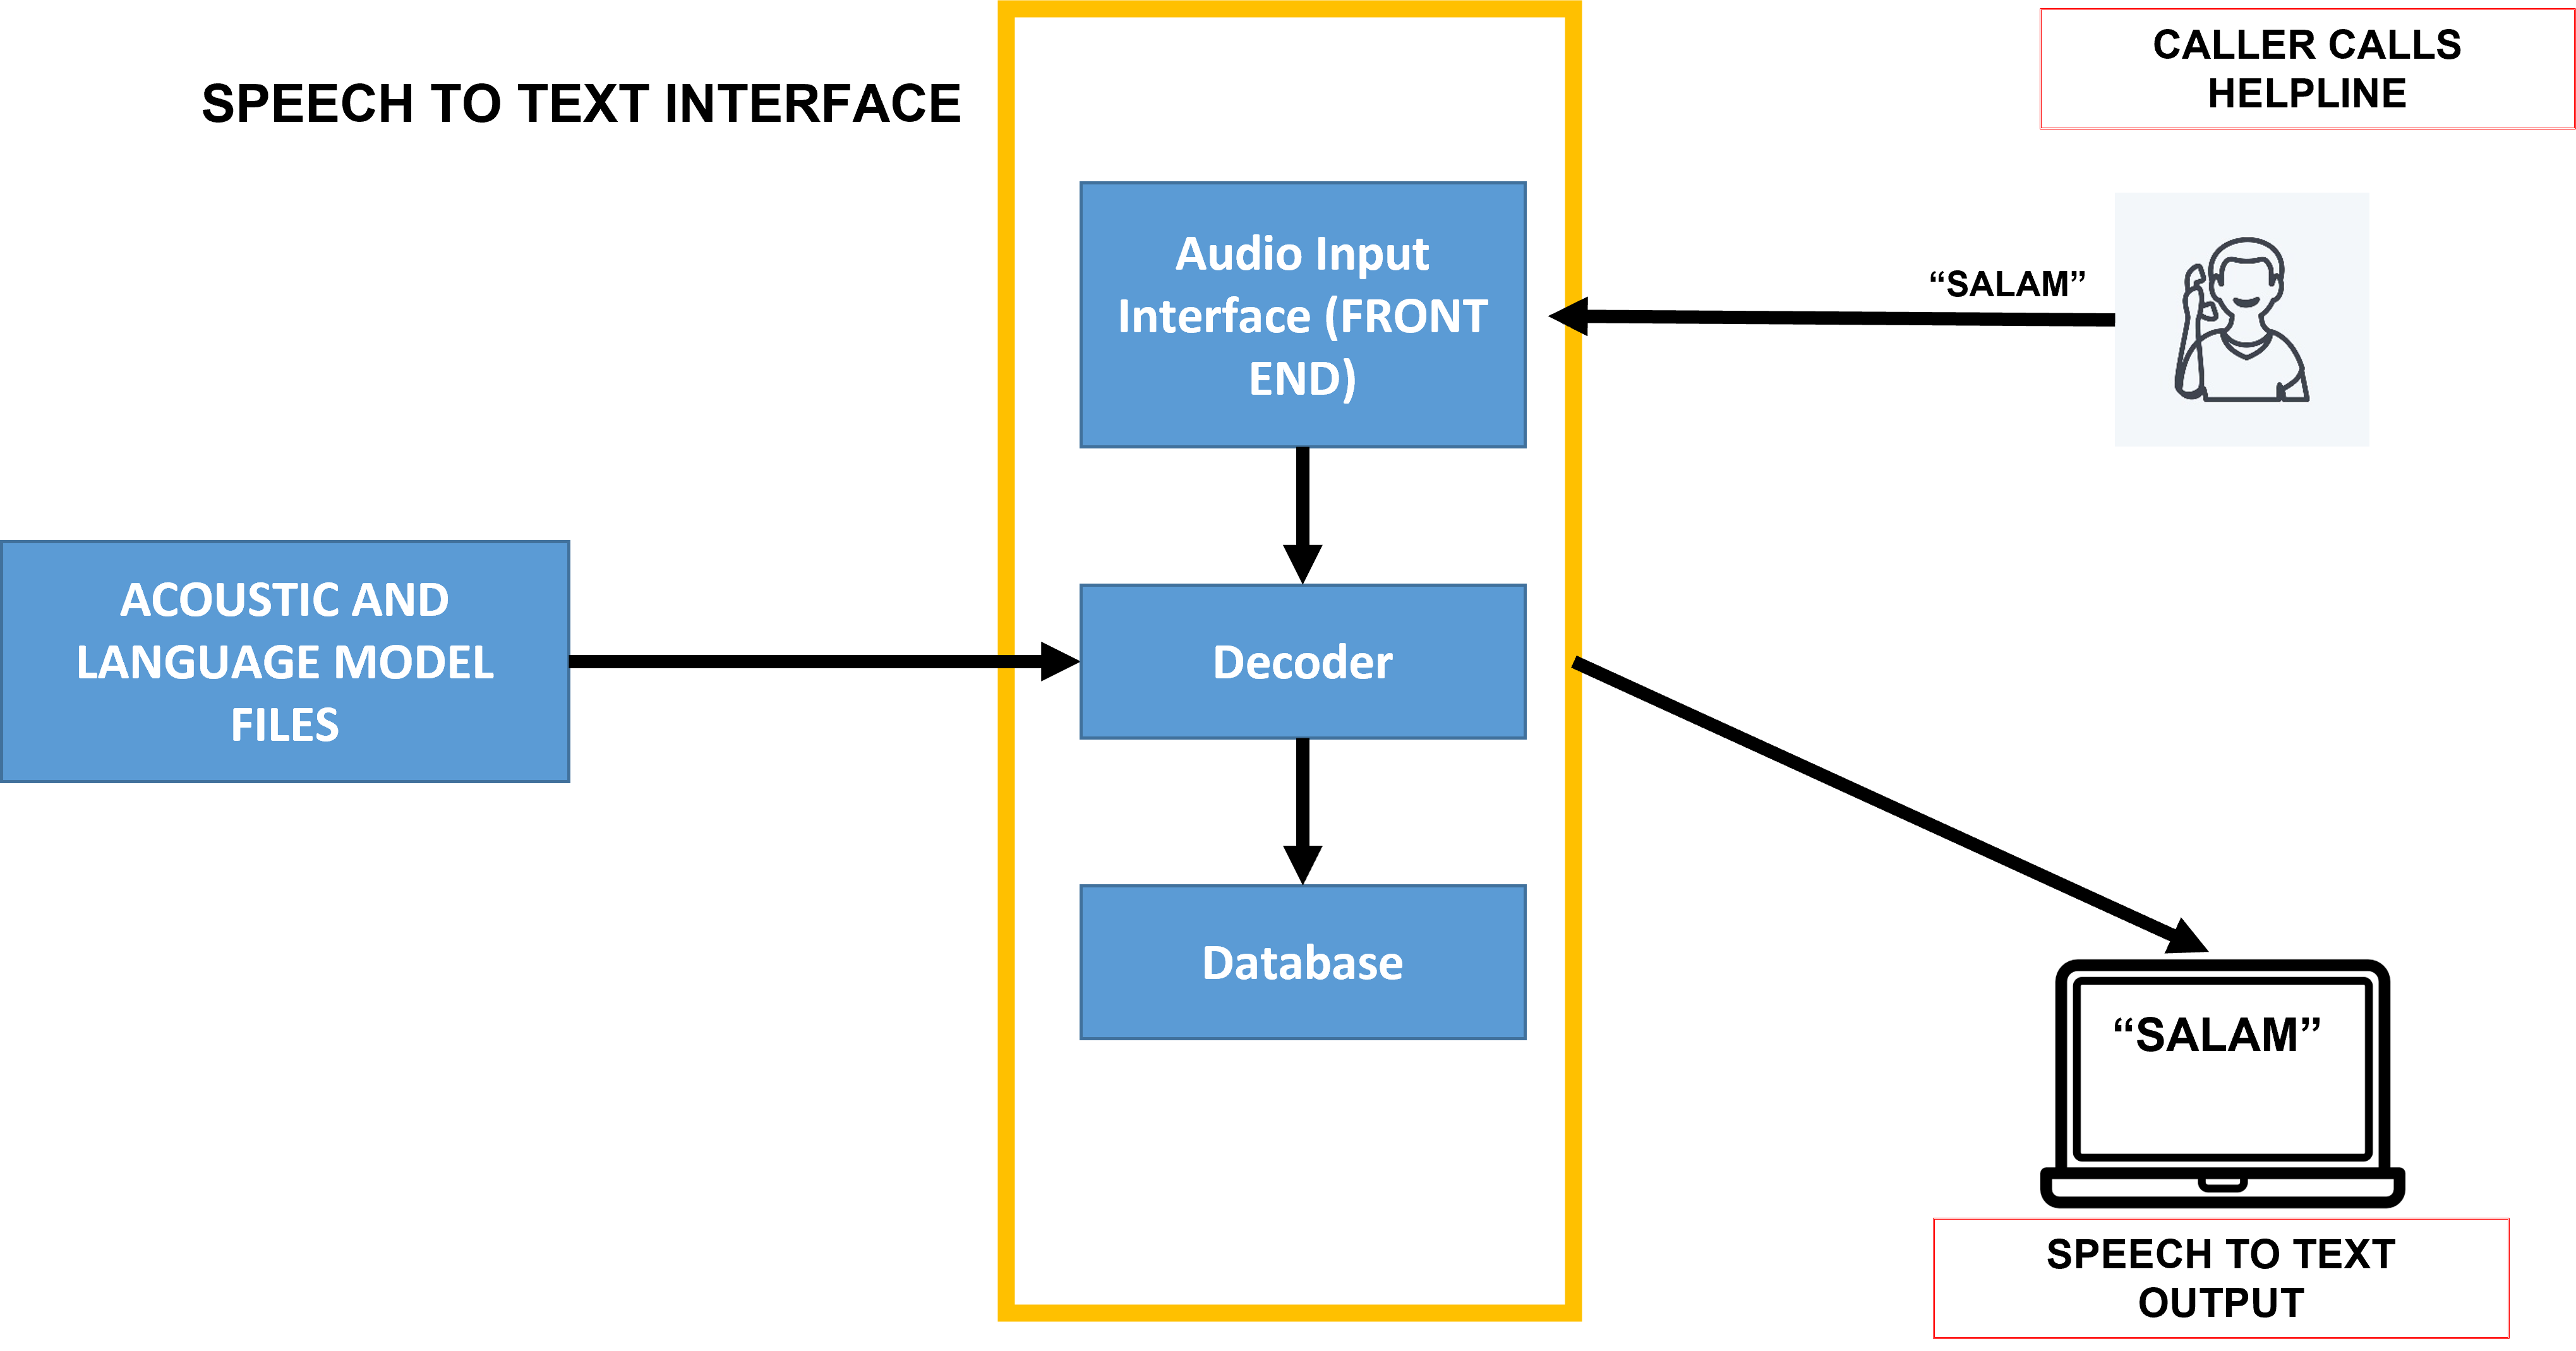
\includegraphics[width=0.9\textwidth]{img/STT2.png}
    \caption{The Speech To Text Interface allows us to take audio input (live or recorded) and it uses the trained model files to give us the text transcription of the audio as output.}
    \label{fig:STT-working}
\end{figure}   

%\begin{figure}[htb]
%    \centering
%    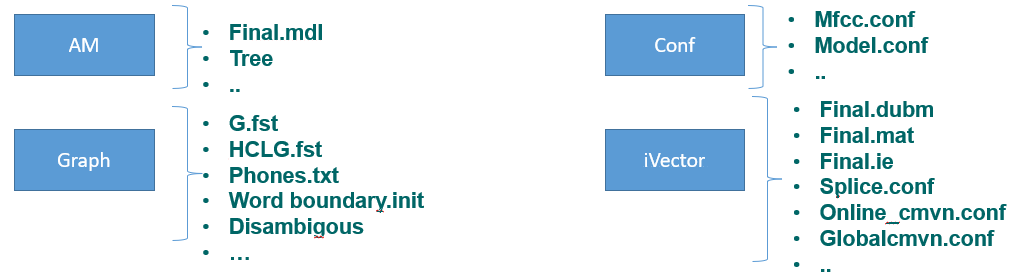
\includegraphics[width=0.7\textwidth]{img/vosk-lm.png}
%    \caption{Model Directory Structure for Speech To Text Interface}
%    \label{fig:vosk-directory-structure}
%\end{figure}    

ASR engines produce very huge model files which add to computational load, storage problems and cross platform deployment issues. We needed an interface that utilizes the necessary language and acoustic model files and provides Speech To Text services on audio signals (live or recorded),  reducing size of the model making it portable and cross-platform compatible. 

We used an offline speech recognition library that comes with a set of accurate models, scripts, and practices and provides ready-to-use speech recognition for different platforms like mobile applications or Raspberry Pi since the model size reduced from 1-5GB to 50-500MB. We can also use this Platform to build a life-long learning platform \cite{eeckt_continual_2021} which continuously improves speech recognition for major languages and use cases \cite{alphacep_vosk_2022}.

    %!TEX root = ../thesis.tex
\chapter{Results and Discussion} % (fold)
\label{cha:results}
In this chapter we will go through our experimental setup and results followed by a detailed analysis and comparison with relevant work.

\section{Experimental Setup} % (fold)
\label{sec:Implementation}

For implementation of our methodology, we used a Dell T7910, Dual Xeon Processors E5-2680 V4 @ 2.4GHz, RTX 3080Ti GPU, 32GB RAM, Ubuntu 20.04 Operating System as shown in Figure \ref{fig:experimental-setup}. We installed the CUDA matrix library to access GPU-based matrix operations to be able to run required parts of GPU computation. We installed a GPU-accelerated primitives library for DNN called NVIDIA CuDNN which provides highly fine-tuned standard routines implementations like forward-backward convolution, pooling, normalization, and activation layers which gives effective performance with CNNs.

We used Kaldi ASR \cite{daniel_povey_kaldi_nodate} Toolkit for the preparation of Language and Acoustic Models and Training of ASR (using Chain nnet3 CNN-TDNN) as shown in Figure \ref{fig:implementation-architecture}. Kaldi is an open source research speech recognition toolkit that implements many state-of-the-art algorithms. Kaldi is currently one of the most tested and cited ASR engines with a very supportive open-source community dedicated to the development and expansion of the project. Various sources show that it still outperforms its contemporaries \cite{christian_gaida_comparing_2014} \cite{georgescu_performance_2021}.

Dataset was divided into test and train as explained in section \ref{sec:Data_preprocessing}. Language Models were prepared using SRILM as explained in section \ref{sub:language_model}. Audio slicing and pre-processing were done using SoX, FFMPEG and Audacity. Monophone and Triphone HMM-GMM Training utilized Open FST, ATLAS and BLAS/LAPAC libraries where as in the Chain CNN-TDNN we used NVIDIA's CUDA and CuDNN for GPU Computation. The scripts used in this were mostly bash, C++ and Python. 

%It has scripts in various languages like C++, bash, perl, python etc. We needed a system that could use the relevant model files from Kaldi and make it easy to deploy in a client-server environment. Kaldi is in C++ primarily and since most of the applications now are python based, we wanted a python based solution for better ease of cross-platform deployability.

ASR Model training produces a lot of Language and Acoustic Model Files which can be an issue during deployment and leads to cross-platform compatibility problems which is why we needed a STT interface that could utilize the model files and give us flexibility and ease of deployment for which we used an open-source offline STT tool called Vosk \cite{alphacep_vosk_2022}. This required us to have python available since this portion is primarily python based.

\newpage
\begin{landscape}

\begin{figure}[htbp]
    \centering
    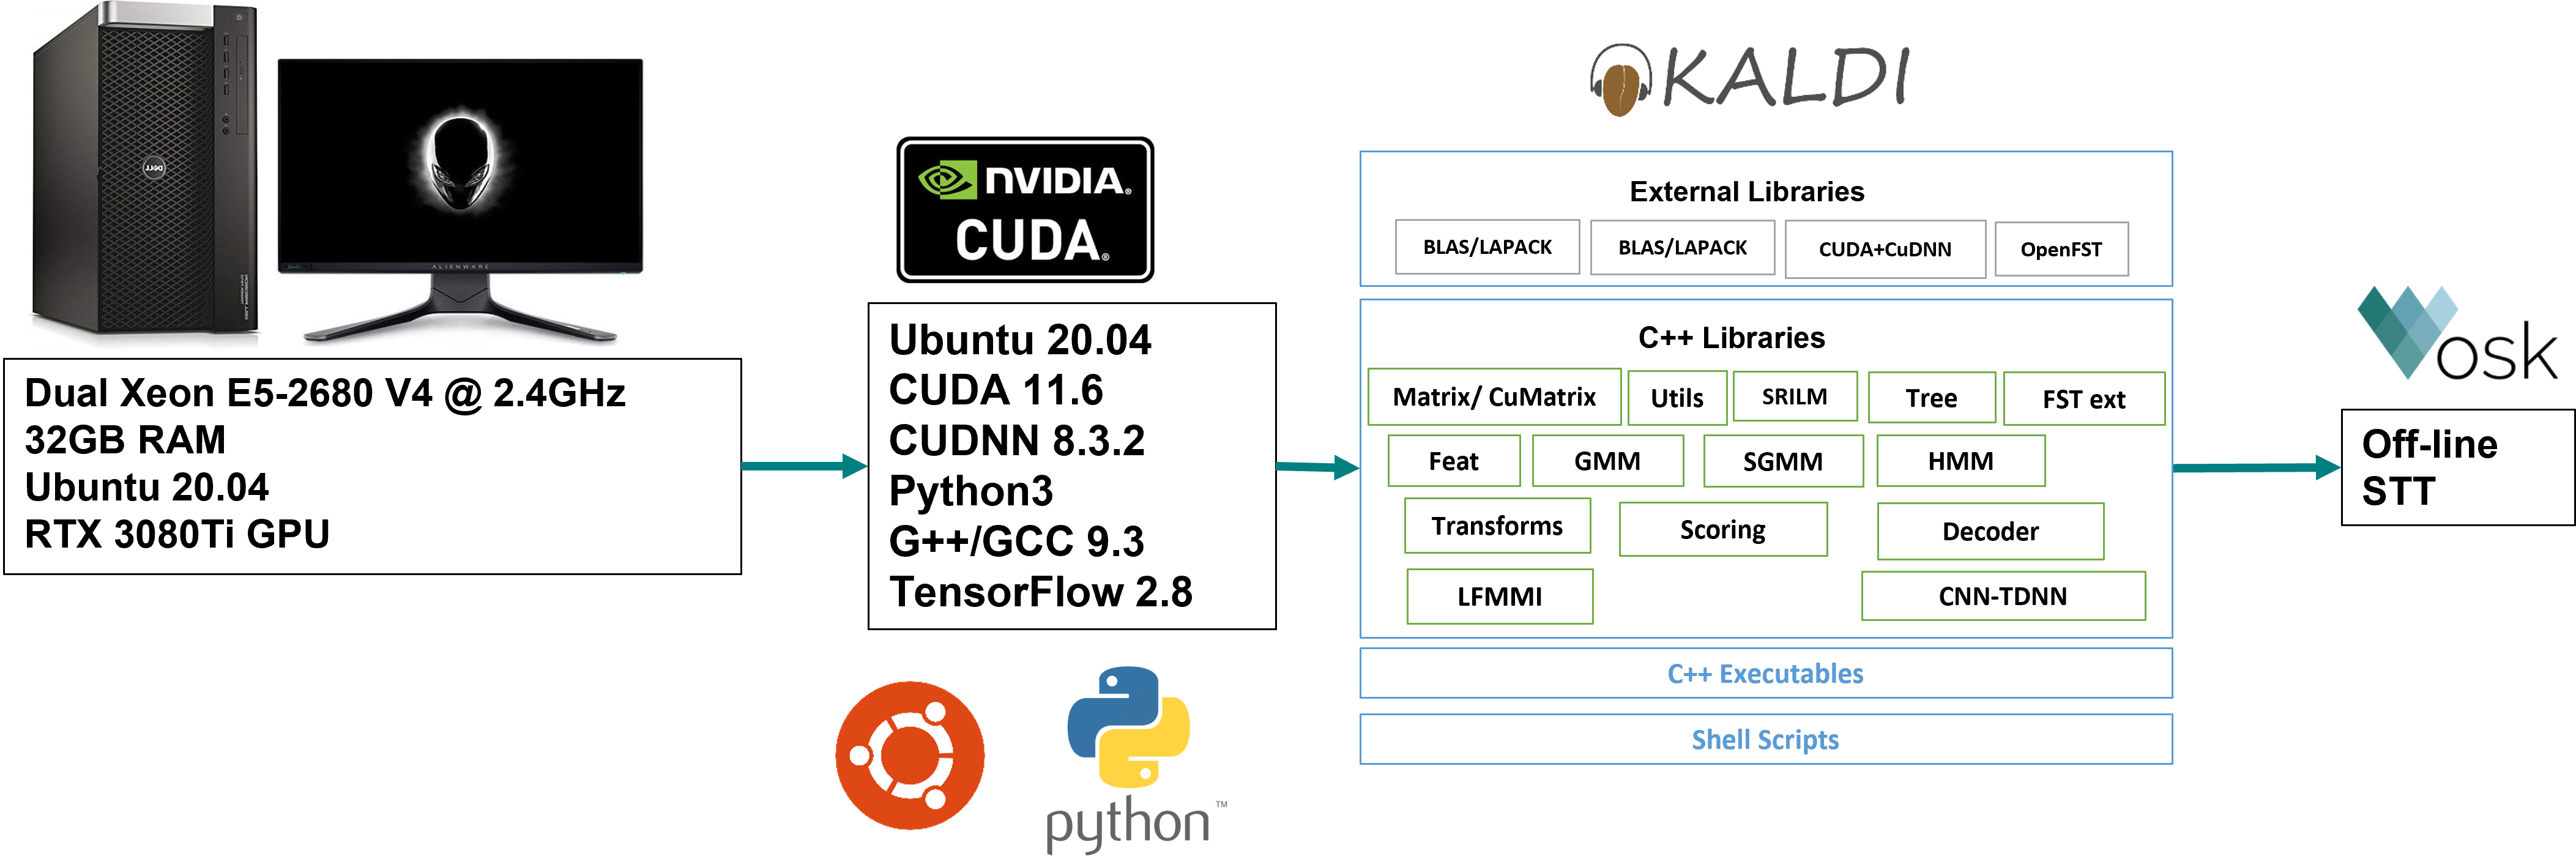
\includegraphics[width=1.5\textwidth]{img/Implementation.png}
    \caption{Experimental Setup}
    \label{fig:experimental-setup}
\end{figure}
\newpage
\begin{figure}[htbp]
    \includegraphics[width=1.5\textwidth]{img/Implement2.png}
    \caption{Implementation Architecture}
    \label{fig:implementation-architecture}
\end{figure}

\newpage
\end{landscape}

\section{Experimental Results}

\begin{table}[h!]
    \centering
    \caption{Our Results} 
    \label{tab:our_result}

    \begin{tabularx}{\textwidth} { 
  | >{\raggedright\arraybackslash}X 
  | >{\raggedright\arraybackslash}X 
  | >{\raggedright\arraybackslash}X | }
    \hline
    \textbf{Data-set} & \textbf{METHOD} & \textbf{RESULTS} \\
    \hline
    Data-set \ref{sub:datasources} D(1-4) & HMM GMM TRIPHONE & WER 13\% and SER 31.2\%  \\ 
    \hline
    Data-set \ref{sub:datasources} D(1-4) & LFMMI CNN-TDNN & WER 5.2\% and SER 20.45\%  \\
    \hline
    Data-set \ref{sub:datasources} D(5) & LFMMI CNN-TDNN & 5.2\%\\   
    \hline
    \end{tabularx}    
\end{table}

We were able to acheive 13\% WER and SER of 31.2\% using HMM-GMM and with CNN-TDNN using LFMMI Objective Function we achieved 5.2\% WER and 20.45\% SER on clean and noisy code-switched Urdu audio data with read speech, spontaneous speech, isolated words and isolated digits. The details of our results is shown in table \ref{tab:our_result}. 

For Evaluation we used WER and SER. While the option of using CER was there we found it irrelevant for us since we are more concerned with the accuracy of words and sentences. The Urdu word \textit{"Janbaaz"} can also be written as \textit{"Jaanbaaz"} or \textit{"Jaanbaz"} and will be spelled pretty much in the same way. Hence, as long as the overall word is accurate and the sentences are accurately transcribed, our ASR is suits our requirements.

It must be noted that Call center audio used for testing was totally unseen, containing OOVs, overlapping and low-volume speech. In audible speech signal areas with no overlap and clean speech (whether single word or long sentences) we were able to achieve WER 5.2\%. but in the overlapping areas, lower volumes, incomplete or partial speech by the speaker and OOVs, the performance degraded yielding 74\% result. 

\section{Comparison with Relevant Work} % (fold)
\label{sec:comparison_result}

For comparison purpose, we used only WER as evaluation metric since we only had WER available in those work as shown in Table \ref{tab:comparison-table}. Our Call Center data is not openly available and hence cannot be used as a metric to compare performance with others. However we can use \cite{ali_automatic_2015}, \cite{sehar_gul_detecting_2020} and \cite{qureshi_urdu_2021} for bench-marking since their data was available and applied in works other than ours. 

%The catch is that most of these tests were conducted using the same set of audio recordings: namely a corpus called Switchboard, which consists of a large number of recorded phone conversations spanning a broad array of topics. Switchboard has been used in the field for many years and is nearly ubiquitous in the current literature—so it’s a reasonable choice. By testing against the same audio corpus, researchers can make apples-to-apples comparisons between themselves and competitors. (Google is the exception; it uses its own, internal test corpus, which is opaque to outsiders).

All these works focused on one of the aspects of ASR input i.e. read speech, isolated words or digits and spontaneous speech. In our case all of these scenarios were covered which makes it more applicable in practical sense.

The works in comparison were all tested primarily on clean audio, making it unsuitable for noisy telephonic environment. In our case the model performed with 5.2\% WER in noisy and clean environment. However in overlapped, improper pronunciations and low volume speech, our model was unable to perform well.

These works focused on pure Urdu words which means they are not applicable for telephonic environment since languages are spoken in code-switched manner. We were able to identify words usage patterns based on Call Center scenario to cover maximum possible vocabulary, trained with noisy and clean samples of same word set to cover maximum possible scenario. We also solved the code-switching problem by keeping a unified written script i.e. Roman. So all English or Urdu words were in Roman script which eased the lexicon building and language modelling process. 

One of the drawbacks of \cite{sehar_gul_detecting_2020} that we identified was that it used very little data-set to train Urdu ASR with Deep Learning. In our case we had limited access to labelled dataset and most of our dataset was unlabelled for which we trained a Hybrid HMM-DNN ASR which was able to use statistical alignments and Neural Networks to train accurate ASR on limited dataset. This approach is suitable for Low-Resource Languages where labelled dataset is not easily available.

Other works mentioned in Chapter \ref{cha:literature_review} cannot be fairly compared (though provided as a reference for bench-marking in future based on available data) because the data-sets are not consistent. For that kind of comparison we need a data-set for Urdu like \cite{godfrey_switchboard_1992}, \cite{garofolo_john_s_timit_1993} and \cite{panayotov_librispeech_2015} on which we can apply various models with same experimental environment and conditions. The results from those training on the common dataset will be able to prove which model works best in noisy/ telephonic environment for Urdu Language. A performance comparison like \cite{georgescu_performance_2021} can then be done on the common data-set for better comparison and analysis.

\begin{landscape}
 
\begin{xltabular}{1.5\textwidth}{|l|X|X|X|}
\caption{Comparison with relevant work} \label{tab:comparison-table} \\

\hline \multicolumn{1}{|c|}{\textbf{Author}} & \multicolumn{1}{c|}{\textbf{Data-set}} & \multicolumn{1}{c|}{\textbf{Method}} & \multicolumn{1}{c|}{\textbf{Reults}} \\ \hline 
\endfirsthead

\multicolumn{4}{c}%
{\tablename\ \thetable{} -- continued from previous page} \\
\hline \multicolumn{1}{|c|}{\textbf{Author}} & \multicolumn{1}{c|}{\textbf{Data-set}} & \multicolumn{1}{c|}{\textbf{Method}} & \multicolumn{1}{c|}{\textbf{Results}} \\ \hline 
\endhead

\hline \multicolumn{4}{|r|}{{Continued on next page}} \\ \hline
\endfoot

\hline
\endlastfoot
    Our Work & Data-set \ref{sub:datasources} D(1-5) & HMM GMM TRIPHONE & WER 13\% and SER 31.2\%  \\ 
    \hline
    Our Work & Data-set \ref{sub:datasources} D(1-5) & LFMMI CNN-TDNN & WER 5.2\% and SER 20.45\%  \\   
    \hline
    Qasim \cite{qasim_urdu_2016} & 139 District names of Pakistan, 300 speakers & HMM & Accent Dependent 60.06\% \newline Accent Independent 75.25\% \\
    \hline
    Hazrat Ali \cite{ali_automatic_2015} & 205 isolated words (20 Speakers) & HMM &  WER 33\% \\
    \hline
    Sehar Gul \cite{sehar_gul_detecting_2020} &  250 words each by 10 speakers \newline 86 sentences by 25 people \newline 100+86 sentences 25 people \newline & Deep Learning (E2E CTC) using DeepSpeech & Accuracy 60\% \newline 56.7\% \newline 51.6\% \\
    \hline
    Zoraiz Qureshi \cite{qureshi_urdu_2021} & PRUS\cite{zia_pronouncur_2018} 708 sentences data set with 5 speakers & GMM/HMM& Accuracy 65\%-75\% (WER 25-35\%) \\
    \hline
    Naeem \cite{naeem_subspace_2020} & Dataset by RUMI and CSALT and NUCES - clean Mono-16000Hz & MONO \newline Tri-1 \newline Tri-2 \newline Tri-3 \newline SGMM \newline (HMM-GMM-SGMM) & WER 3.24\% SER 64.26\% \newline WER 16.70\% SER 52.41\% \newline WER 16.74\% SER 52.80\% \newline WER 13.63\% SER 52.62\% \newline WER 9.64\% SER 48.53\% \\
    \hline
\end{xltabular}
\end{landscape}

\section{Analysis of Results}
\label{se:discussion}

From the perspective that we set out initially to improve work of \cite{sehar_gul_detecting_2020}, our model has clearly out-performed on Sehar's Data-set of malicious Urdu sentences and on general code-switched Urdu conversations as well. 

The works we studied for Urdu ASR were tested to perform generally in clean environment on one of the following: Isolated words, Isolated Digits, Read speech or spontaneous speech. Our work was able to perform with 95\% accuracy on all these types of speech in a noisy as well as in clean environment. We found that most of the previous work generally focused on using pure Urdu words or sentences. The fact remains that Urdu is never spoken in pure form. It is always spoken in code-switch to English, Panjabi and other local languages as well in normal conversation. 

\subsection{Addressing Code Switching issue}

The usual idea for speech to text output may be to use local script for the transcription text and in Urdu it is usually Nastaliq. However, to address the code-switching issue we kept the written script as Roman instead of making Urdu Nastaliq and Roman English separately allowing us to bypass the requirement of building separate Language and Phonetic Models for every word of a different language used. Keeping one writing script for code-switched Low resource language will help solve the issue of Language modelling, saving a lot of time to structure and map data, while also reducing the Model complexity. 

Our Model was able to recognize numbers and write them down in Arabic Numeral scripts which was due to the fact that we mapped the numbers to their pronunciations in our Lexicon. In situations where the speech include series of number, the ASR used arabic numeral as text output instead of their English pronunciation which is a result we have not seen before in a code-switched Urdu ASR. 

\subsection{Data Centric Approach}

Based on our results, our approach clearly out-performed the usual model-centric approach. We built our ASR from scratch which meant that Data Pre-Processing also has to be iteratively audited (as seen in figure \ref{fig:datacentric-ML-approach}) along with model tweaking. This is one of the key reasons why our model performed better.It also provided us following advantages \cite{noauthor_data-centric_nodate}:
\begin{itemize}
    \item Improved accuracy by effectively using data as a strategic asset to ensure more precise estimates, observations, and decisions.
    \item Complex data transformations are eliminated.
    \item Data inconsistencies and errors are reduced.
    \item Data redundancy is reduced.
    \item Data quality and reliability is improved.
    \item Expenses are reduced since less time and effort is required to work on model building and tweaking.
\end{itemize}

\subsection{Data-set Diversity}

We added a unique diversity in our data-set which covered maximum possible scenarios in our call center ASR. Our data performed optimally in all the following points (English and Urdu):
\begin{itemize}
    \item Isolated Digits
    \item Isolated words 
    \item Urdu Malicious sentences (Section \ref{sub:datasources} from D2)
    \item Read Speech (Words and Digits) of duration up to 20 seconds
    \item Spontaneous Speech (Words and Digits) of duration up to 20 seconds
    \item Clean Audio
    \item Noisy or Telephonic Audio
    \item Audio lengths. The feature extraction of the input signal is limited by the memory of GPUs in use, it is best to slice all audio files not to exceed 30 seconds, as it is a reasonable input size for batching.
\end{itemize}

Other models we studied in our literature review performed in on or two of the above points. Our model is the first that covers all these scenarios. This model works as a speaker independent model.

The best approach for a resource constraint scenario is to take small data-set of 10-20 hours. We accurately label it to build a strong language model. It is best to understand the context of data-set and do an analysis of the language usage e.g. for code-switching, common words, jargon etc. Then train a strong model which can then annotate the remaining data-set which can then be used to train Deep Learning Model which is known to improve as data-set size increases. The golden data-set we will eventually have as we accurately label and integrate more and more data will become our asset. 

Models will evolve for the better but data-set is the same (mostly a standard). Hence it is always best to build up the data-set instead focusing on model only.

\subsection{The Role of Chain CNN-TDNN Approach}
HMM-DNN method involves use of statistical model to build up Language and acoustic models. These alignments can be used to further train and improve model using Neural Networks. In a way it uses the accuracy of Statistical Models on low data-sets and the scalability of Neural Networks together. 

We used CNN-TDNN for Neural Network Training with LF-MMI Objective function which has previously shown to work better on noisy data-sets \cite{daniel_povey_kaldi_nodate}\cite{abdel-hamid_convolutional_2014} \cite{zorila_investigation_2019} \cite{biswas_semi-supervised_2019} \cite{noauthor_tdnn_nodate} \cite{georgescu_kaldi-based_2019} \cite{kreyssig_improved_2018}. This architecture has CNN Layers followed by TDNN Layers which both add certain benefits in the Training pipeline.

If the input features are noisy, having a few CNN layers (2D CNN) before TDNN (which is basically a time dialated 1-dimension CNN) blocks at the input would help the model learn some non-linear transformations which can reduce the effect of the noise on speech input. TDNNs are basically temporal convolution whereas CNNs are convolutions in both frequency and space dimensions, which gives it the capability to learn patterns better.

TDNN works well in Speech Processing compared to other Neural Networks as they can be tuned easily as compared to LSTMs, and gives 11.4\% WER than the baseline TDNN's 12.1\% WER on the Switchboard \cite{godfrey_switchboard_1992} part of Eval2000 data-set \cite{daniel_povey_kaldi_nodate}. 

Speech Recognition requires a system that takes care of temporal context and time delay neural network architecture captures long term temporal dependencies better than a feed-forward DNN does. We need to look at features left and right i.e. contexting and we need better prediction of phoneme states which is why for Low Resource Languages TDNNs work best. 

The LF-MMI or chain model helped reduce the training time of the model and allowed for more efficient and effective training which improved accuracy from HMM-GMM Triphone training by 8\% in our case. It makes best use of GPU and avoids using branching or pruning tree search. 

The process of creating the denominator FST is very similar to that of a traditional decoding graph creation, however the computation of the denominator forward-backward computation are parallelized by the GPU. The process is sped up by performing careful optimizations, including reversal, weight pushing, and minimization followed by epsilon removal on the denominator FST to minimize graph size.

Hence this reduces graph size and improves training speed an performance while using Neural Networks, in comparison to pure Deep Learning based models. It is also applicable on streaming data.

%This model can be trained directly without word lattice of pre-training because LF-MMI uses:
%\begin{itemize}
%\item Phone Level Language Model usually 4-gram instead of 
%\item No LM Smoothing to avoid introduction of multiple states
%\item 30ms frames in feature extraction instead of 10ms
%\item One state per phone instead of 3   
%\end{itemize}

\subsection{Speech To Text System Interface Integration}
We identified based on relevant work from our literature review that Model Files that are generated are often huge in Size which causes difficulty in deployment. Our proposed framework utilized a Speech To Text Interface that would use relevant files giving it flexibility, ease of cross-platform deployment and scalability \cite{alphacep_vosk_2022}.

Using Kaldi and Vosk \cite{alphacep_alphacepvosk-server_2022} allows us to built accurate offline speech recognition supporting four major communications protocols i.e. MQTT, GRPC, WebRTC, and Websocket. Server can be locally used to provide speech recognition to smart homes and PBXs such as free-switch or asterisk and can also deployed as a back-end for web-based streaming speech recognition, as well as to power chat-bots, websites, and telephony.

%The idea behind STT interface like Vosk is that the neural network-based speech recognizers require a huge amount of speech data for training and enormous computing power and time to train and optimize the parameters. Neural networks have problems with human-like one-shot learning, their decisions are not very robust to unseen conditions and are hard to understand and correct. 

%Thus, a system based on large signal database concept was built in which audio fingerprinting scheme is applied. The audio is segmented on chunks, the chunks are stored in the database based on LSH hash value. During decoding the system looks up the chunks in the database to get the possible phones which helps it to make a proper decision on decoding results.

%Neural network-based speech recognizers require a huge amount of speech data for training and enormous computing power and time to train and optimize the parameters. Neural networks have problems with human-like one-shot learning, their decisions are not very robust to unseen conditions and are hard to understand and correct. 

%Thus we need a system that is built based on large signal database concept in which audio fingerprinting scheme is applied. The audio is segmented on chunks, the chunks are stored in the database based on LSH hash value. During decoding the system looks up the chunks in the database to get the possible phones which helps it to make a proper decision on decoding results.

%The \textbf{advantages} of this approach are:
%\begin{itemize}
%    \item It can quickly train on more than ten thousand hours of speech data on very simple hardware
%    \item It can easily correct recognizer behavior just by adding samples
%    \item It can make sure that recognition result is correct because it is sufficiently represented in the training data-set
%    \item It can parallelize training across thousands of nodes
%    \item It supports lifelong learning paradigm
%    \item It can use this method together with more common neural network %training to improve recognition accuracy
%    \item The system is robust against noise
%\end{itemize}

\section{Shortcomings}
\label{sec:shortcomings}
The Shortcomings can be categorized into following:
\begin{enumerate}
    \item Robustness 
    \item Data-set Limitations
    \item Model Limitations
    \item Speech To Text Interface Limitations
\end{enumerate}

\subsection{Robustness}
Our ASR system faced issues with accuracy in overlapping speech and in longer duration audios. The problem of overlapping speech  is still one of the most difficult in ASR \cite{chen_progressive_2018} and it must be catered in this system. Eventually it will be desirable to go towards E2E solutions which do not require the language structuring. 
\par
However, that can only be done once we have more than 1000 hours of data of labelled speech which is in itself a big project. Without consistent data-set, there is not much that can be said with authority as to which Language or acoustic modelling method works best for Urdu. 
\par 


\subsection{Data set Limitations}
We lacked a standard big data of labelled corpus like Switch Board \cite{godfrey_switchboard_1992} due to which it is not possible to benchmark or compare our performance to other works. Making a standard labelled big data in code-switched Urdu will be very beneficial for researchers working in Urdu ASR. It will help benchmark the performances of various models since data is standard. Roman and Arabic-based Urdu script are required with the audio model to help propel this area of research forward.

\subsection{Limitations of Model}

While HMM-DNN continues to produce cutting-edge results, DNN's role is limited. HMM-DNN has its own limitations which include:
\begin{itemize}
    \item DNN has a limited role and is mostly used for simulation of the posterior state probability of an HMM's hidden state. The time-domain feature is still being modelled by HMM.
    \item Data alignment problem arises when attempting to model time-domain features with RNN or CNN instead of HMM since loss functions of RNNs and CNNs are defined at each point in the sequence, hence the alignment relationship between the RNN output sequence and the target sequence must be known in order to perform training \cite{backstrom_introduction_2022}.
    \item It has a complex structure that includes several components such as the acoustic model, language model, and pronunciation model. Each system component is independently optimized with a different objective function, usually resulting in a suboptimal global solution. Hence, it requires linguistic resources like a handcrafted pronunciation dictionary prone to human error \cite{hussein_arabic_2022}. 
    
\end{itemize}

\begin{figure}[htb]
    \centering
    \includegraphics[width=0.8\textwidth]{img/ComparisonASRMODELS.png}
    \caption{Comparison of Three ASR Training Approaches} %For lower training datasets Traditional methods work well but E2E outperforms with bigger training data-sets.}
    \label{fig:comparison-all-asr-approach}
\end{figure}

\subsection{Speech To Text Interface Limitations}
We designed the system for use in a desktop or high-end client-server environment but the best usage of this will be deployment in edge devices as the world moves towards Edge computing and Internet of Things. This model at present is not deployed for self-supervised learning and federated machine learning or life-long learning method \cite{dautume_episodic_2019} \cite{chang_towards_2021}.

%It is built based on large signal database concept in which audio fingerprinting scheme and the \textbf{disadvantages} to this approach are \cite{alphacep_vosk_2022}:
%\begin{itemize}
%    \item The index is really huge, it is not expected to fit a memory of single server.
%    \item The generalization capabilities of the model are quite questionable, at the same time the generalization capabilities of the neural networks are also questionable.
%    \item For now the segmentation requires conventional ASR, but in the future we may need to segment it ourselves.
%\end{itemize}

\section{Future Work} % (fold)
\label{sec:future-work}

\begin{itemize}
    \item Model requires robustness in overlapping or distorted speech areas. To cater for robustness we will also need to expand this model to integrate approaches like Parametric and Adaptive models \cite{shrawankar_adverse_2013}. 
    \item Multilingual model training to integrate more languages which are locally spoken like Panjabi, Sindhi etc. The script can be kept Roman instead of Arabic to reduce language modelling complication.
    \item STT interface requires own code for segmentation of audio and it also requires Specialized hardware to implement this AI paradigm \cite{alphacep_vosk_2022}.
    \item Self-supervised training integration requires exploration  \cite{yang_online_2022}.
    \item Federated Learning and secure application on Edge AI systems need to be explored \cite{noauthor_federated_nodate}.
    \item Expansion of vocabulary, environment, accent and other variations in dataset is essentially required to form a golden dataset on which we can apply various training methods to get the most accurate model. 
    \begin{itemize}
        \item Data should be scaled up to more than 2000 hours eventually for better testing of End to End methods for Code-switched Urdu ASR. 
        \item Models change for the better but dataset is constant which is an asset. If we have a good dataset, we can always train better models with better accuracy and robustness. 
        \item Figure \ref{fig:comparison-all-asr-approach} shows that HMM based model works well with less dataset but with increase in data size, accuracy of Deep Learning is much more than HMM or hybrid models.
    \end{itemize}
    \item Examining Sub-word implementation \cite{smit_advances_2021} for code-switched Urdu and apply other Language Modelling methods like RNN, to test if this model can be improved.
        \begin{itemize}
            \item Slavic Languages e.g. Estonian, Nordic Languages E.g Finnish and Arabic Languages are highly inflected languages which requires specific components for modelling inflection e.g. factored language model. 
            \item An effective method is to use Sub Word Implementation \cite{smit_advances_2021} which has shown to improve accuracy more for Arabic language compared to English. 
            \item Arabic Language, as a case study, has a concept of base words comprising of three letters from which other words are derived.
            \begin{itemize}
                \item E.g. \RL{علم} (pronounced as Ilm) means knowledge which is base word. The word \RL{معلم} (pronounced as Mualim) means teacher or mentor, the connotation means transmitter or sharer of knowledge. 
                \item The essence and the characters or alphabets of the base word \RL{علم} (comprising of 3 alphabets "\RL{ع}" "\RL{ل}" "\RL{م}") remains there as the word compounds and expands. 
                \item If this structure is learned by the Computer through Machine Learning, Machines may be able to capture out-of-vocabulary words more easily. 
            \end{itemize}
        \end{itemize}
    %\item Building a Robust and noise resistant model is still one of the hard problems in ASR.
\end{itemize}



    %!TEX root = ../thesis.tex
\chapter{Conclusion} % (fold)
\label{cha:discussion_conclusion}
%Our work was originally to improve \cite{sehar_gul_detecting_2020} work to detect malicious sentences in Urdu using ASR which used Deep Learning on a very limited self-generated data-set. When we began our initial analysis we realized that instead of working on tweaking the model, it is better to rework the entire structure and adopt a Data-Centric Approach. 

%Not only did we use the original data-set of \cite{sehar_gul_detecting_2020} but we also added data from other sources to enhance the vocabulary and cater for various other factors (\ref{cha:why_asr_difficult}). 

%Initially, We tried using Hindi models from Vosk \cite{alphacep_vosk_nodate-1} and GitHub to transcribe our call center audios. It gave us 99\% WER. We also tested our audio files on Google Speech Recognition API \cite{zhang_uberi_speechrecognition_nodate} which resulted in the same. Note that Google SR has Hindi libraries available, not Urdu. Hence, we had to develop our model specifically for our environment (keeping in mind our time, manpower and budget constraints).

%We trained an ASR with data of variety in terms of duration, noisiness and language using Hybrid system with Chain CNN-TDNN. With less available data-set we were able to utilize the state of the art structure of traditional models and flexibility and scalability of Chain CNN-TDNN training method. 

%We had a lot of unstructured data and some open source data-set available and we kept a more Data Centric approach. The fact that we kept our data well labelled saved most of the trouble when training the model.

%Instead of cleaning the Call Center audio to retain speech data, we tailored our data-set such that for the same alphabet, number and word we have a noisy as well as a clean sample available which would then be used to train the ASR. In this way the system had instances of how a word sounded like in a clean environment and in a noisy telephonic environment. Our approach catered for various constraints like Timeline, budget and ease of deployment.

Our work presented a data-centric approach to train a code-switched Urdu ASR using Hybrid HMM-DNN method for noisy telephonic environment in a resource-constrained scenario. We analyzed the call center call content and built our dataset. To cater for the code-switching issue between Urdu and English we used Roman script for Text output. The from various sources mentioned in section \ref{sec:Data_preprocessing} were collected, labelled and processed. We trained a HMM based model followed by Chain CNN-TDNN for model building. This was then linked to a Speech To Text Interface allowing the model to be flexibly used across platforms.

%Urdu is Pakistan's "lingua franca," connecting people who speak regional languages such as Balochi, Pashto, Punjabi, and Sindhi with various dialects. It is spoken by over a hundred million people in Pakistan, India, Bangladesh, and parts of Europe. Despite this, Urdu is a low resource language in ASR field as there is very little publicly available transcribed speech data, text corpus, and pronunciation lexicon. 

A robust speech recognition system generally requires hundreds of hours of transcribed speech data, as well as a massive text corpus and lexicon which is lacking with under-resourced languages like Urdu which is why Urdu speakers are around the world excluded from the benefits of ASR.

We proposed a workable framework that involved generation of statistical modelling and alignment for language and acoustics of speech data and applied Neural Networks to improve the accuracy of ASR system. With only 10 hours of data we were able to achieve up to 5.2\% WER. This results shows that Hybrid HMM-DNN (Chain CNN-TDNN) method is an effective and efficient method for ASR Model training with limited data-set available. 

However the model alone is not the only thing to consider when working on a deployable solution. Our work is one of the few examples that takes a Data-Centric Approach to machine learning and the primary reason why our framework gave good results was due to our focus on improving data before tweaking the model.

We had initially set out, only to improve model of \cite{sehar_gul_detecting_2020} to detect malicious words but we ended up building a solution which not only outperformed on data set from \cite{sehar_gul_detecting_2020,ali_automatic_2015,qureshi_urdu_2021}, but we also managed to improve its performance for read-speech, continuous or spontaneous speech and isolated word utterances in code-switched Urdu environment. Our work however still requires improvement in it's robustness especially in overlapping or unclear or distorted speech signals. 

Our work also took into account various security considerations. In fact security policies and practices with respect to ASR systems is definitely and important research area which can be explored further in future. We integrated an open source Speech To Text Interface that allows the models to be easily deployed in Desktop, IOT devices, Asterisk (open source call center solution) Web and Client-Server Environment. 

Hence the work paved way ahead for putting Code-Switched Urdu ASR in a practical usage to benefit Urdu Speaking people around the world.

    
\bibliography{references.bib}
\bibliographystyle{ieeetr}

%\nocite{*}
\clearpage \pagenumbering{roman}  % This makes the page numbers Roman (i, ii, etc)
%\newpage


%\appendixtitleon
%\appendixname
%\appendixname{Appendix}

%\makeatletter
%\renewcommand{\appendixname}{Appendix}
%\def\@chapapp{Appendix}
%\renewcommand\@chapapp{Appendix}
%\def\chaptername{Appendix}
%\def\appendixname{Appendix}\chaptername{Appendix}
%Chapters.  If there is only
                %one Appendix Chapter, then use \begin{appendix}
%\makeatother
%\begin{appendix}
%\begin{appendices}               % Start of the Appendix



%   %!TEX root = ../thesis.tex

\chapter{The Output}    
\label{App_A}
We will now share our output on our ASR Engine i.e. Kaldi. We will also share our output of Speech To Text on Vosk. Finally we will also share our output in comparison with the Google ASR library \cite{zhang_uberi_speechrecognition_nodate} for our call center test audio.

\begin{landscape}
\begin{figure}[ht]
    \centering
    \includegraphics[width=1.45\textwidth]{img/RESULTS3.jpg}
    \caption{Output on Kaldi}
    \vspace{11pt}
    \includegraphics[width=1.2\textwidth]{img/Results-1.png}
    \caption{Output on Vosk}
    \label{fig:Result_output}
\end{figure}

\begin{figure}[ht]
    \centering
    \includegraphics[width=1.5\textwidth]{img/Results-2.png}
    \caption{Our Result on our test audio data files compared to google ASR \cite{zhang_uberi_speechrecognition_nodate}. Google has Hindi Library in its Python ASR API which is why it is not able to transcribe Code-switched Urdu Audio accurately resulting in a garbage output.}    \label{fig:Result_output_compare}
\end{figure}   
\end{landscape}

\chapter{Sample Audio Pre-Processing Codes}
\label{App_B}

We used SoX and ffmpeg on our Linux System (\ref{sec:Implementation}). Instead of running a command on each, we automated the process by making a bash script which inputs  and output target directory as well as the required extensions and recursively runs the sox or ffmpeg command in all wav or mp3 files found in the directory:
\lstset{style=mycoding}
\begin{lstlisting}[language=bash, caption= Audio Pre-Processing (SoX)]
!# bin/bash
target= echo "Enter target directory: "
read target

extin= echo "enter extension of input audio file: "
read extin

extout= echo "enter extension of output audio file: "
read extout

outch= echo "enter output channel: "
read outch

dest= echo "Enter Destination file name with extension: " #Also can be used for customizing output file name along with extension
read dest

for f in "$target"/*."$extin";
do
    sox --channels "$outch" "$f"."$extin" "$f"-converted."$extout"    
done | awk 'END { printf("File count: %d", NR); } NF=NF' 
\end{lstlisting}


Same could be done with ffmpeg as well if we replace the sox line with:
\lstset{style=mycoding}
\begin{lstlisting}[language=bash, caption= Audio Pre-Processing (ffmpeg)]
ffmpeg -i "$f".wav -ss $start -to $end -c copy "$f"-converted.wav ##time format is 00:00:01 
\end{lstlisting}
 
    %\include{appendix2}
    %\chapter{FPGA CAD Flow}

\section{Design Flow}

    %\chapter{Mapping Capabilities of Spartan-3 FPGA}



\

%\end{appendix}
%\end{appendices} % End of the Appendix Chapters.
%\makeatother
%\chapter{Vita}
Muhammad Danyal Khan
   % Optional Vita, use \begin{vita} vita text \end{vita}

\end{document}